\bookpart{随机变量、分布与因果响应}{Random Variables, Distributions and Causal Responses}
\label{part:probability-stochastic-processes-statistics}
\label{part:random-variables-distributions-and-causality}

\BookPartGuide{%
一次测量会有误差，不同人群会有不同的数据分布，主动安排培训又可能改变结果的生成
方式。这三类问题分别需要随机变量、分布比较和因果响应来描述。本部分沿着它们展开：
先建模单个随机量和随机过程，再比较两个分布，最后检查观测关联何时能支持行动后果
的判断。

第10章“随机变量”建立概率空间上的随机对象、条件关系、分布模型、随机序列与过程，
并说明怎样从样本估计未知量、检验假设和评估估计误差。第11章“随机分布”把研究对象提升为整个
概率分布，讨论信息量、分布差异、最优传输和分布优化，以及参数变化怎样改变分布。
第12章“因果响应”比较不同安排下的结果，并区分给定模型后的计算、数据能否唯一
确定响应，以及怎样推断结果的生成结构。

三章分别处理随机对象、分布之间的关系和机制改变后的响应。条件分布能够描述已观察
信息下的不确定性，分布距离能够比较两套规律，但二者都不会自动给出干预结论；因果
响应还需要说明行动具体改变什么、结果怎样生成，以及数据怎样收集。}

\chapter{随机变量}
\label{chap:random-variables}
\label{chap:probability-theory}
\label{chap:stochastic-processes-and-approximation}
\label{chap:mathematical-statistics}

同一台传感器重复测量一个稳定信号，读数却不完全相同。怎样描述一次读数的可能取值？两台设备一起测量时，共同的环境扰动怎样改变平均结果？增加测量次数能否消除误差，又能否据此保证下一次读数落在一个窄区间内？这些问题都围绕随机变量展开，但所求的对象并不相同。

随机变量是把基础结果变成数值的可测映射；观测得到的是这张映射的一次取值，分布则记录各种取值出现的概率。本章先在概率规律给定时描述变量、关系与变换，再研究重复观测的累计误差及时间过程。最后把分布改成未知对象，讨论样本能支持怎样的估计、预测与检验。平均准确、路径接近和统计覆盖分别有自己的条件，不能相互替代。随机噪声进入状态递推、随机积分和状态方程的内容由第~\ref{chap:dynamical-systems-and-state-estimation}章承接。

\section{随机变量的定义}
\label{sec:rv-definition}
\label{sec:probability-representation-conditioning}
描述读数之前，需要明确概率赋给哪些事件、读数怎样从事件产生。完整分布、均值方差和参数化模型是描述同一对象的不同层次；少量摘要通常不能还原完整分布。

\subsection{概率空间上的随机变量}
\label{sec:probability-spaces-random-variables}
% Baseline P:24-61
设一次带噪观测只能取有限个结果\(\Omega=\{\omega_1,\ldots,\omega_m\}\)，并为每个结果指定权重\(p_j\geq0\)，满足\(\sum_{j=1}^{m}p_j=1\)。事件
\(A\subseteq\Omega\)的概率为
\[ \mathbb{P}(A)=\sum_{\omega_j\in A}p_j. \]
这个有限公式已经包含三条基本规则：概率非负，全集概率为\(1\)，互不相交事件的概率可以相加。一般样本空间可能不可数，而且未必希望给每个子集都赋概率。第~\ref{chap:mathematical-analysis}章的测度语言恰好把这三条规则推广到这种情形。

\begin{definition}[概率空间]
  \label{def:probability-space}
\term{概率空间}（probability space）是三元组\((\Omega,\mathcal{F},\mathbb{P})\)。其中，\(\Omega\)是所有可能结果组成的
样本空间，\(\mathcal{F}\)是事件组成的\(\sigma\)代数，\(\mathbb{P}:\mathcal{F}\to[0,1]\)是满足
\(\mathbb{P}(\Omega)=1\)的测度。可数可加性说明，对两两不交的事件\((A_j)_{j\geq1}\)，
\[ \mathbb{P}\left(\bigcup_{j\geq1}A_j\right)
  =\sum_{j\geq1}\mathbb{P}(A_j). \]
\end{definition}
概率不是附着在口头描述上的数，而是定义在指定事件族上的测度。若改变\(\mathcal{F}\)，能够询问的事件也会改变。

对事件\(A\)，其补事件和单调性分别给出
\[ \mathbb{P}(A^{\mathsf c})=1-\mathbb{P}(A),
  \qquad A\subseteq B\Longrightarrow\mathbb{P}(A)\leq\mathbb{P}(B). \]
概率测度还与单调极限相容。若\(A_n\uparrow A\)，令
\(B_1=A_1\)、\(B_n=A_n\setminus A_{n-1}\)，则\((B_n)\)两两不交且
\(A=\bigcup_nB_n\)。可数可加性因而给出
\[
  \mathbb{P}(A)
  =\sum_{n\geq1}\mathbb{P}(B_n)
  =\lim_{n\to\infty}\mathbb{P}(A_n).
\]
若\(A_n\downarrow A\)，对补事件使用上一结论便得到
\(\mathbb{P}(A_n)\to\mathbb{P}(A)\)。第二个结论用到了
\(\mathbb{P}(A_1)\leq1<\infty\)；对一般无限测度，递减连续性必须另外要求起始集合具有有限测度。

对任意可数事件族，即使事件不互斥，也有联合界
\begin{equation}
  \mathbb{P}\left(\bigcup_{j\geq1}A_j\right)
  \leq
  \sum_{j\geq1}\mathbb{P}(A_j).
  \label{eq:probability-union-bound}
\end{equation}
第~\ref{sec:probability-random-functions-uniform-error}节会用它同时控制有限候选的误差。
% Baseline P:65-78
\begin{definition}[随机变量]
  \label{def:probability-random-variable}
给定可测空间\((\mathcal{X},\mathcal{A})\)，若映射
\(X:\Omega\to\mathcal{X}\)满足
\(X^{-1}(B)\in\mathcal{F}\)对每个\(B\in\mathcal{A}\)成立，就称\(X\)为取值于
\(\mathcal{X}\)的\term{随机变量}（random variable）。
\end{definition}
对实值变量，只需验证
\[ \{\,\omega:X(\omega)\leq x\,\}\in\mathcal{F},
  \qquad x\in\mathbb{R}, \]
因为这些半无限区间生成\(\mathcal{B}(\mathbb{R})\)。可测性保证由取值范围定义的
原像确实属于\(\mathcal{F}\)，因而有概率。随机变量不是“本身会随机变化的符号”，而是把基础结果转换成所关心对象的可测函数。

\begin{definition}[随机向量]
\label{def:rv-random-vector}
\(d\)维\term{随机向量}是从\((\Omega,\mathcal F,\mathbb P)\)到
\((\mathbb R^d,\mathcal B(\mathbb R^d))\)的可测映射
\(\bm X=(X_1,\ldots,X_d)^\top\)。它等价于各坐标可测，不包含坐标相互独立的假设。一般随机对象只需把取值空间换成指定的可测空间。
\end{definition}

例如令\(\Omega=\{a,b,c,d\}\)，四种设备状态等概率出现，规定
\[
\begin{array}{c|rrrr}
\omega&a&b&c&d\\ \hline
X(\omega)&9&9&11&11\\
Y(\omega)&9&11&9&11
\end{array}
\]
基础结果\(b\)不是读数\(9\)；\(X\)不是某一次得到的\(9\)，而是整张读数规则。事件
\(\{X=9\}=\{a,b\}\)的概率为\(1/2\)。两次使用同一规则不等于两次结果相同，也不自动意味着独立抽样；重复实验的联合规则还要另行给出。
图~\ref{fig:rv-objects}把这些层次及未知规律下的推断目标分开。
\begin{figure}[htbp]
  \centering
  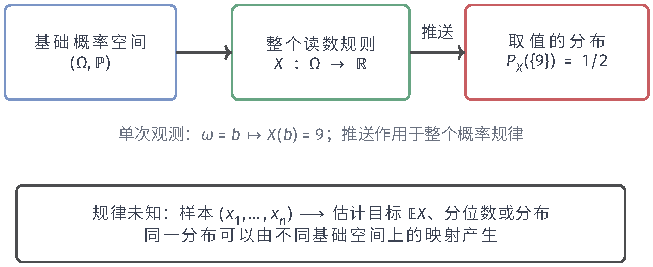
\includegraphics[width=\linewidth]{figures/01-mathematical-preliminaries/04-random-variables-distributions-and-causality/tikz/rv-objects/figure.pdf}
  \caption{基础结果经随机变量映射成为读数；把事件概率推送到取值空间得到分布。分布未知时，样本用于估计指定目标，并不能唯一还原基础空间上的映射。}
\label{fig:rv-objects}
\end{figure}

\subsection{随机变量的分布表示}
\label{sec:rv-distribution}
\label{sec:probability-radon-nikodym-change-measure}
% Baseline P:79-101
\(X\)在实数轴上诱导的概率测度称为它的\term{分布}（distribution）：
\[ \mathbb{P}_X(B)
  =\mathbb{P}(X\in B),\qquad B\in\mathcal{B}(\mathbb{R}). \]
分布函数
\[ F_X(x)=\mathbb{P}(X\leq x) \]
单调不减、右连续，并满足\(\lim_{x\to-\infty}F_X(x)=0\)与\(\lim_{x\to\infty}F_X(x)=1\)。反过来，每个具有这些性质的函数都对应某个实随机变量的分布。

若\(\mathbb{P}_X\)集中在可数点集上，可写成概率质量函数\(p_X(x)=\mathbb{P}(X=x)\)。若它相对于Lebesgue测度有密度\(f_X\)，则
\[ \mathbb{P}(X\in B)=\int_B f_X(x)\,\mathrm{d}x,
  \qquad F_X(x)=\int_{-\infty}^{x}f_X(t)\,\mathrm{d}t. \]
密度值不是单点概率。连续分布通常满足\(\mathbb{P}(X=x)=0\)，但
\(f_X(x)\)仍可为正；在密度连续的点，它等于小邻域概率除以邻域长度后的局部极限；一般密度只在几乎处处意义下确定，不能在任意指定点都作这样的解释。
例如\(X\)在区间\([0,1/4]\)上均匀分布时，\(f_X(x)=4\mathbb{I}\{0\leq x\leq1/4\}\)。
密度值\(4\)可以大于\(1\)，因为概率由面积而非高度给出：
\(\mathbb{P}(0.10\leq X\leq0.15)=4\times0.05=0.2\)，而每个单点的概率仍为\(0\)。

图~\ref{fig:probability-density-cdf}把这一区分放在同一个分布上：密度图中的矩形面积，正是分布函数在区间两端的增量。因而从分布函数求区间概率不需要把连续结果变成单点概率。

\begin{figure*}[htbp]
  \centering
  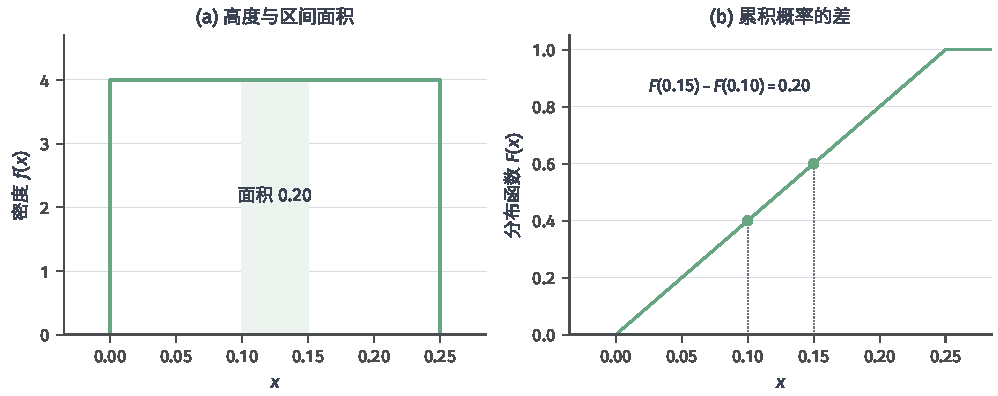
\includegraphics[width=\linewidth]{figures/01-mathematical-preliminaries/04-random-variables-distributions-and-causality/matplotlib/probability-density-cdf/figure.pdf}
  \caption{区间\([0,1/4]\)上的均匀分布（解析式教学图）。左图阴影为\([0.10,0.15]\)的概率\(0.20\)，密度高度为\(4\)；右图的概率是\(F(0.15)-F(0.10)\)，两个端点本身均没有正概率质量。}
  \label{fig:probability-density-cdf}
\end{figure*}
% Baseline T:953-962
\term{\(q\)分位数}（quantile）可定义为
\[
  F^{-1}(q)=\inf\{y:F(y)\geq q\},\qquad 0<q<1.
\]
这个广义逆为给定的\(F\)和\(q\)选出唯一的下分位数。更一般地，所有满足分位数
不等式的点组成集合
\[
  \mathcal Q_q=\{a:F(a^-)\leq q\leq F(a)\}.
\]
当\(F\)在水平\(q\)上存在平坦区间时，这个集合可能包含多个点；上述广义逆约定选取其中的下端代表。

在刚才的四状态例子中，若把基础概率依次改成
\((0.1,0.2,0.3,0.4)\)，读数规则及取值范围都不变，但
\(\mathbb P(X=9)\)从\(1/2\)变成\(0.3\)。所以“能取哪些值”和“以什么概率取值”是两个问题。离散质量是相对于计数测度的密度；连续密度通常相对于Lebesgue测度，密度的数值不能脱离参考测度解释。
% Baseline P:136-246

熟悉的密度以Lebesgue测度为参照，概率质量函数以计数测度为参照。
两种写法共同的问题是：能否用一个参考测度下的权重表示另一个测度？
绝对连续排除参考测度完全看不到的正质量区域，Radon--Nikodym导数在这一前提下给出权重。
换测度随后复用同一个权重公式，而不必对每个分布重新推导积分。

\par\medskip\noindent\textbf{绝对连续与零集兼容性}\quad
在有限集合上，两个概率表\((p_j)\)与\((q_j)\)可以逐项比较。若想用\(P\)下的样本计算\(Q\)下的平均，候选权重自然是\(q_j/p_j\)。但当\(p_j=0\)而\(q_j>0\)时，
\(P\)永远不会产生第\(j\)个结果，任何有限权重都无法补回这部分质量。

这一障碍在一般空间中由绝对连续刻画：参考测度看不到的集合，目标测度也不能给它
正质量。
\begin{definition}[测度的绝对连续]
\label{def:probability-absolute-continuity}
设\(\nu\)与\(\mu\)为同一可测空间\((\Omega,\mathcal{F})\)上的测度。若
\[ \mu(A)=0\Longrightarrow\nu(A)=0,
  \qquad\text{对所有 }A\in\mathcal{F}\text{成立}, \]
则称\(\nu\)对\(\mu\)\term{绝对连续}（absolute continuity），记作\(\nu\ll\mu\)。
\end{definition}
它只要求\(\mu\)的零集也是\(\nu\)的零集，并不表示\(\nu(A)\leq\mu(A)\)，
也不自动提供有界的密度比。

\par\medskip\noindent\textbf{有限分割上的密度表示}\quad
先设\(\mu\)与\(\nu\)为有限测度，取有限可测分割
\(\Omega=A_1\mathbin{\dot\cup}\cdots\mathbin{\dot\cup}A_m\)，并假设\(\nu\ll\mu\)。
对\(\mu(A_j)>0\)的分块定义
\[ r(\omega)=\frac{\nu(A_j)}{\mu(A_j)},
  \qquad \omega\in A_j; \]
在\(\mu(A_j)=0\)的分块上令\(r=0\)。绝对连续性保证后一类分块也满足\(\nu(A_j)=0\)。因此，对任意由这些分块组成的事件\(A\)，
\[ \nu(A)=\int_A r\,\mathrm{d}\mu. \]
对在各分块上取有限实常数的函数\(g\)，逐项相加还给出
\begin{equation}
  \int_{\Omega}g\,\mathrm{d}\nu
  =
  \int_{\Omega}gr\,\mathrm{d}\mu.
  \label{eq:probability-finite-change-measure}
\end{equation}
一般定理要做的事，是在没有预先给定有限分块时构造同样的\(r\)
\scite{math-kallenberg2021probability}

\begin{theorem}[Radon--Nikodym定理]
\label{thm:probability-radon-nikodym}
设\(\mu\)与\(\nu\)是\((\Omega,\mathcal{F})\)上的\(\sigma\)有限测度，且
\(\nu\ll\mu\)。则存在非负可测函数\(r\)，使每个\(A\in\mathcal{F}\)都满足
\begin{equation}
  \nu(A)=\int_A r\,\mathrm{d}\mu.
  \label{eq:probability-rn-representation}
\end{equation}
函数\(r\)在\(\mu\)-几乎处处意义下唯一，记为\(r=\mathrm{d}\nu/\mathrm{d}\mu\)，称为\term{Radon--Nikodym导数}
（Radon--Nikodym derivative）。
\end{theorem}

\begin{proof}
先设\(\mu,\nu\)有限，并令\(\lambda=\mu+\nu\)。在线性空间
\(L^2(\lambda)\)上定义
\[
  T(f)=\int f\,\mathrm{d}\nu.
\]
由于\(\nu\leq\lambda\)，Cauchy--Schwarz不等式给出
\[
  |T(f)|
  \leq\int|f|\,\mathrm{d}\nu
  \leq\nu(\Omega)^{1/2}
       \left(\int f^2\,\mathrm{d}\nu\right)^{1/2}
  \leq\nu(\Omega)^{1/2}\lVert f\rVert_{L^2(\lambda)}.
\]
因此\(T\)是有界线性泛函。由第~\ref{chap:functional-analysis-and-approximation}章的Riesz表示定理，存在
\(g\in L^2(\lambda)\)，使
\[
  \int f\,\mathrm{d}\nu=\int fg\,\mathrm{d}\lambda,
  \qquad f\in L^2(\lambda).
\]
取\(f=\mathbb{I}_A\)可得\(\nu(A)=\int_Ag\,\mathrm{d}\lambda\)。若
\(A=\{g<0\}\)具有正测度，则对集合\(\{g\leq-1/k\}\)取指示函数会得到
\(\nu(\{g\leq-1/k\})<0\)的矛盾，故\(g\geq0\)几乎处处。又因为
\(\mu(A)=\lambda(A)-\nu(A)=\int_A(1-g)\,\mathrm{d}\lambda\geq0\)，同理有
\(g\leq1\)几乎处处。

令\(C=\{g=1\}\)。在\(C\)上有
\(\mu(C)=\int_C(1-g)\,\mathrm{d}\lambda=0\)，而\(\nu\ll\mu\)推出
\(\nu(C)=0\)。另一方面，\(\nu(C)=\int_Cg\,\mathrm{d}\lambda=\lambda(C)\)，所以
\(\lambda(C)=0\)。于是可以在其余部分定义
\[
  r=\frac{g}{1-g},
\]
并在\(C\)上任取值。由
\(\mathrm{d}\mu=(1-g)\,\mathrm{d}\lambda\)，对每个\(A\in\mathcal{F}\)都有
\[
  \int_A r\,\mathrm{d}\mu
  =\int_A\frac{g}{1-g}(1-g)\,\mathrm{d}\lambda
  =\int_Ag\,\mathrm{d}\lambda
  =\nu(A).
\]

若\(r_1,r_2\)都满足该表示，则对
\(A_k=\{r_1\geq r_2+1/k\}\)有
\[
  0=\int_{A_k}(r_1-r_2)\,\mathrm{d}\mu
  \geq\frac{1}{k}\mu(A_k),
\]
故\(\mu(A_k)=0\)。对\(k\)取并集得到\(r_1\leq r_2\)几乎处处；交换二者即得唯一性。

对\(\sigma\)有限的\(\mu,\nu\)，分别取有限测度覆盖并求交，可以把\(\Omega\)写成可数个互不相交、在两种测度下均有限的可测分块。在每个分块上使用上述构造，再把各块导数拼接，便得到全空间上的\(r\)。拼接后的表示可先对有限个分块验证，再由单调收敛推广到全部分块。
\end{proof}

这个证明先让\(\lambda=\mu+\nu\)同时支配两种测度，再把测度\(\nu\)表示为
\(L^2(\lambda)\)中的函数\(g\)。绝对连续性只用于排除\(g=1\)承载正质量，保证比值
\(g/(1-g)\)能够成为相对于\(\mu\)的密度。构造得到的是可测密度，并没有得到逐点上界。


\subsection{随机变量的整体特征}
\label{sec:rv-features}
\label{sec:probability-expectation-conditional-expectation}
\label{sec:probability-moment-transforms}
% Baseline P:105-132
对非负随机变量\(X\)，定义
\[ \mathbb{E}[X]
  =\int_{\Omega}X(\omega)\,\mathrm{d}\mathbb{P}(\omega). \]
对一般实随机变量，写\(X=X^+-X^-\)。当
\(\mathbb{E}[|X|]<\infty\)时，正负两部分积分都有限，此时称\(X\)可积，并定义
\(\mathbb{E}[X]=\mathbb{E}[X^+]-\mathbb{E}[X^-]\)。不要求可积便随意相减\(\infty-\infty\)没有意义。

期望只依赖\(X\)的分布。对可测函数\(g\)，只要\(g(X)\)非负或可积，就有
\begin{equation}
  \mathbb{E}[g(X)]
  =
  \int_{\mathbb{R}}g(x)\,\mathrm{d}\mathbb{P}_X(x).
  \label{eq:probability-lotus}
\end{equation}
离散时右侧是\(\sum_x g(x)p_X(x)\)，有密度时则是\(\int g(x)f_X(x)\,\mathrm{d}x\)。这条“无须先求\(g(X)\)分布”的积分公式，会反复用于矩、蒙特卡洛估计和分布变换。

式~\eqref{eq:probability-lotus}直接来自推送测度的定义。对指示函数
\(g=\mathbb{I}_B\)，等式两侧分别为
\(\mathbb{P}(X\in B)\)与\(\mathbb{P}_X(B)\)，所以相等。线性性把结论推广到非负简单函数；任取递增到非负可测\(g\)的简单函数列，再在两侧使用单调收敛定理，即得非负情形。可积实值函数则分别对\(g^+\)和\(g^-\)应用这一结论。这个证明同时说明，等式并不要求\(X\)有密度。

\begin{example}[带噪观测的平均目标]
\label{ex:probability-noisy-observation}
设未知信号为\(\theta\)，观测为
\[ Y=\theta+\varepsilon,
  \qquad\mathbb{E}[\varepsilon]=0. \]
只要\(\varepsilon\)可积，就有\(\mathbb{E}[Y]=\theta\)。这并未说明一次读数接近
\(\theta\)，也未说明多个读数的平均必然收敛；后者还需要抽样依赖关系和矩条件。概率模型先把目标写成分布下的平均，后续误差结论再回答有限观测能否逼近这个平均。
\end{example}
% Baseline P:419-422
可积随机变量的均值记作\(\mu_X=\mathbb{E}[X]\)。若\(\mathbb{E}[X^2]<\infty\)，其方差为
\[ \operatorname{Var}(X)
  =\mathbb{E}\bigl[(X-\mu_X)^2\bigr]=\mathbb{E}[X^2]-\mu_X^2. \]
% Baseline P:832-853

均值和方差便于计算，却不足以区分许多分布。若关心偏斜、尾部或独立和的分布变化，需要在这两个摘要之外保留信息：高阶矩增加摘要阶数，生成函数则把一系列摘要组织到一个函数中。

若\(\mathbb{E}[|X|^k]<\infty\)，则\(\mathbb{E}[X^k]\)称为\(k\)阶原点矩，
\(\mathbb{E}[(X-\mathbb{E}X)^k]\)称为\(k\)阶中心矩。三阶中心矩反映不对称性，四阶中心矩反映尾部与峰度，但有限低阶矩通常不能唯一确定分布。

\begin{definition}[矩母函数与累积量生成函数]
  \label{def:probability-moment-generating-functions}
设\(X\)为实随机变量。若存在\(\delta>0\)，使\(\mathbb E e^{tX}<\infty\)对全部\(|t|<\delta\)成立，则在该邻域上定义\term{矩母函数}（moment-generating function, MGF）为
\[ M_X(t)=\mathbb{E}[e^{tX}]. \]
\term{累积量生成函数}（cumulant-generating function）是
\[ K_X(t)=\log M_X(t). \]
\end{definition}
若可在积分号下求导，则\(M_X^{(k)}(0)=\mathbb{E}[X^k]\)。
矩存在却不保证矩母函数在原点邻域有限。取密度为
\(e^{-z^2/2}/\sqrt{2\pi}\)的标准高斯变量\(Z\)，令\(X=e^Z\)；
这样得到的正随机变量称为对数正态变量（lognormal random variable）。
对每个正整数\(k\)，配方得到
\[
 \mathbb E X^k
 =\frac1{\sqrt{2\pi}}\int_{\mathbb R}e^{kz-z^2/2}\,\mathrm dz
 =e^{k^2/2}<\infty.
\]
但对任意\(t>0\)，指数矩的被积函数是
\(e^{te^z-z^2/2}/\sqrt{2\pi}\)。当\(z\to+\infty\)时，\(e^z\)的增长压过\(z^2\)，
该被积函数最终大于\(1\)，所以在正半轴上的积分发散。
因此\(\mathbb E e^{tX}=\infty\)，虽有全部正整数阶矩，仍不满足上述邻域条件。
累积量生成函数的前两阶导数分别给出均值和方差。对随机向量\(\bm{X}\)，
\[ K_{\bm{X}}(\bm{t})
  =\log\mathbb{E}\bigl[e^{\bm{t}^{\top}\bm{X}}\bigr], \]
混合偏导数给出联合累积量。独立变量的变换函数乘积及累积量可加法则在第~\ref{sec:rv-combinations}节说明。

% Baseline P:856-870
前两阶关系可以直接核对。若存在\(\delta>0\)，使
\(\mathbb E e^{tX}<\infty\)对全部\(|t|<\delta\)成立，则在更小邻域内，
\(|X|e^{tX}\)与\(X^2e^{tX}\)可由邻域端点的指数函数控制。第~\ref{chap:mathematical-analysis}章的积分下求导条件于是给出
\[
  M_X'(t)=\mathbb{E}[Xe^{tX}],\qquad
  M_X''(t)=\mathbb{E}[X^2e^{tX}].
\]
因为\(M_X(0)=1\)，
\[
  K_X'(0)=\frac{M_X'(0)}{M_X(0)}=\mathbb{E}X,
  \qquad
  K_X''(0)
  =M_X''(0)-M_X'(0)^2
  =\operatorname{Var}(X).
\]
矩母函数可能在零点的任何双侧邻域都不有限。研究分布极限时，需要一个对所有实参数都存在的变换。
% Baseline P:875-878
\begin{definition}[特征函数]
  \label{def:probability-characteristic-function}
实随机变量\(X\)的特征函数为\(\varphi_X(t)=\mathbb E e^{\mathrm i tX}\)，其中\(t\in\mathbb R\)。随机向量的版本为\(\varphi_{\bm X}(\bm t)=\mathbb E e^{\mathrm i\bm t^\top\bm X}\)。复数期望分别对实部与虚部积分。
\end{definition}
由于复指数的绝对值恒为\(1\)，特征函数总存在。它用振荡而非指数放大取值，因此与可能发散的矩母函数承担不同职责；后面将用它把独立和的分布极限转成函数的逐点极限。

变换还有一个有限低阶矩所没有的性质：保留完整的特征函数，就保留了分布。
\begin{theorem}[变换函数的分布唯一性]
\label{thm:rv-transform-uniqueness}
同维随机向量的特征函数在所有实向量参数上相同，当且仅当它们的分布相同。
若两个矩母函数都在原点的某个共同开邻域内有限，并在该邻域内相同，
它们也确定相同的分布。
\end{theorem}
这里引用概率变换的唯一性定理，不展开所需的Fourier反演论证
\scite{math-kallenberg2021probability}
它把“两个变换相同”转成“两个分布相同”；只比较有限个矩或有限个参数点，
没有这种唯一性保证。

\subsection{常见取值空间的分布模型}
\label{sec:probability-common-distributions}
\label{sec:probability-families-transformations}
分布模型首先应与观测含义相容：一次成功标记、固定次数中的成功数、等待时间和随机比例具有不同取值空间。取值空间相容仍不代表模型正确，例如非负整数并不自动服从Poisson分布；独立性、齐次性和尾部形状都要由问题另行支持。

\subsubsection{离散取值下的分布模型}
% Baseline P:885-902
\term{Bernoulli分布}以参数\(p\in[0,1]\)描述一次二元结果：
\[ \mathbb{P}(X=x)=p^x(1-p)^{1-x},
  \qquad x\in\{0,1\}, \]
且\(\mathbb{E}X=p\)、\(\operatorname{Var}(X)=p(1-p)\)。\(n\)个独立同分布的
Bernoulli变量之和服从\term{二项分布}
\[ \mathbb{P}(S=k)
  =\binom{n}{k}p^k(1-p)^{n-k},\qquad k=0,\ldots,n, \]
其均值和方差分别为\(np\)与\(np(1-p)\)。

若一次试验有\(K\)个类别，概率向量\(\bm{p}\)满足\(p_k\geq0\)及\(\sum_kp_k=1\)。\(n\)次独立试验的类别计数\(\bm{N}\)服从\term{多项分布}，质量为
\[ \mathbb{P}(\bm{N}=\bm{n})
  =\frac{n!}{\prod_{k=1}^{K}n_k!}\prod_{k=1}^{K}p_k^{n_k},\qquad\sum_{k=1}^{K}n_k=n. \]
其均值为\(\mathbb{E}N_k=np_k\)，协方差为\(\operatorname{Cov}(N_j,N_k)=n(p_j\mathbb{I}\{j=k\}-p_jp_k)\)。

\term{Poisson分布}以\(\lambda>0\)描述固定窗口中的稀疏计数：
\[ \mathbb{P}(N=k)
  =e^{-\lambda}\frac{\lambda^k}{k!},\qquad k=0,1,\ldots, \]
且均值、方差都为\(\lambda\)。独立计数的相加规律在第~\ref{sec:rv-combinations}节推导。

类别变量\(C\in\{1,\ldots,K\}\)满足
\(\mathbb P(C=k)=p_k\)，称为类别分布。类别编号只是标记，编号的均值通常没有物理含义；用独热向量
\(\bm e_C\)表示时，其均值就是概率向量\(\bm p\)。多项分布描述多次独立类别抽取后的整组计数。
Poisson计数没有固定的最大次数；二项计数的上界则是已知试验次数\(n\)。二者不能只按均值接近就视为同一个模型。

\subsubsection{连续取值下的分布模型}
% Baseline P:908-913
\term{指数分布}以速率\(\lambda>0\)描述等待时间，密度为
\[
f_T(t)=\lambda e^{-\lambda t}\mathbb I_{\{t\geq0\}}.
\]
其均值为\(1/\lambda\)、方差为\(1/\lambda^2\)，并有无记忆性：
\[ \mathbb{P}(T>s+t\mid T>s)=\mathbb{P}(T>t). \]
无记忆性只适用于已经等待的时长不改变剩余等待分布，不表示不同等待时间自动独立。
它与Poisson事件计数的联系在第~\ref{sec:rv-poisson}节给出过程定义后建立。
% Baseline P:927-1014
\term{高斯分布}（Gaussian distribution，也称正态分布）
\(X\sim\mathcal{N}(\mu,\sigma^2)\)具有密度
\[ f_X(x)
  =\frac{1}{\sqrt{2\pi\sigma^2}}\exp\left\{-\frac{(x-\mu)^2}{2\sigma^2}\right\},\qquad \sigma^2>0. \]
其均值为\(\mu\)，方差为\(\sigma^2\)。当\(a\neq0\)时，仿射变换满足\(aX+b\sim\mathcal{N}(a\mu+b,a^2\sigma^2)\)；当\(a=0\)时，结果是集中于\(b\)的点质量，可记作退化高斯，但不能再使用上面的正方差密度。

正变量上的密度常含有\(x^{a-1}e^{-bx}\)这一形状。要把它归一化，需要一个依赖形状参数的积分常数。
\begin{definition}[Gamma函数]
  \label{def:probability-gamma-function}
对实数\(a>0\)，定义Gamma函数为
\begin{equation}
  \Gamma(a)=\int_0^\infty t^{a-1}e^{-t}\,\mathrm dt,
  \qquad a>0.
  \label{eq:probability-gamma-function}
\end{equation}
\end{definition}
\(a>0\)保证零附近的幂函数可积，指数衰减保证无穷远处可积。
分部积分给出\(\Gamma(a+1)=a\Gamma(a)\)，并且\(\Gamma(1)=1\)，所以对正整数
\(n\)，有\(\Gamma(n)=(n-1)!\)。它把阶乘延伸到这里需要的正实参数，而换元
\(t=bx\)说明\(\int_0^\infty x^{a-1}e^{-bx}\,\mathrm dx=\Gamma(a)/b^a\)。

形状参数\(a>0\)、速率参数\(b>0\)的\term{Gamma分布}密度为
\[ f_X(x)
  =\frac{b^a}{\Gamma(a)}x^{a-1}e^{-bx}\mathbb{I}\{x>0\}. \]
其均值为\(a/b\)，方差为\(a/b^2\)。指数分布是\(a=1\)的特例。若使用尺度参数
\(\vartheta=1/b\)，公式会改变；引用Gamma分布时必须说明采用速率还是尺度参数。

若\(U\sim\operatorname{Gamma}(a,1)\)与\(V\sim\operatorname{Gamma}(b,1)\)独立，则
\[ R=\frac{U}{U+V} \]
服从\term{Beta分布}\(\operatorname{Beta}(a,b)\)。为得到归一化常数，令
\(S=U+V\)，于是\(U=RS\)、\(V=(1-R)S\)，变换的Jacobian绝对值为\(s\)。独立Gamma密度经过换元得到
\[
  f_{R,S}(r,s)
  =
  \frac{r^{a-1}(1-r)^{b-1}}{\Gamma(a)\Gamma(b)}
  s^{a+b-1}e^{-s},
  \qquad 0<r<1,\ s>0.
\]
对\(s\)积分并使用Gamma函数定义，得到
\[
  f_R(r)
  =
  \frac{\Gamma(a+b)}{\Gamma(a)\Gamma(b)}
  r^{a-1}(1-r)^{b-1}\mathbb{I}\{0<r<1\}.
\]
因此
\[
  \mathbb{E}R=\frac{a}{a+b},\qquad
  \operatorname{Var}(R)=
  \frac{ab}{(a+b)^2(a+b+1)}.
\]
Beta分布适合描述\([0,1]\)上的随机比例。
这里共同速率使比例与总量分离；两个Gamma变量速率不同则不能直接得到该Beta结论。

当\(K\geq2\)、每个\(\alpha_k>0\)时，独立变量\(G_k\sim\operatorname{Gamma}(\alpha_k,1)\)的归一化比例
\[ P_k=\frac{G_k}{\sum_{j=1}^{K}G_j} \]
服从下面定义的Dirichlet分布。其均值为
\(\mathbb{E}P_k=\alpha_k/\alpha_0\)，其中\(\alpha_0=\sum_k\alpha_k\)。同样令
\(S=\sum_kG_k\)，把前\(K-1\)个比例和总量作为新坐标；Jacobian为
\(s^{K-1}\)。联合密度分成一个形状为\(\alpha_0\)的Gamma密度和一个比例密度。这给出：
\begin{definition}[Dirichlet分布]
  \label{def:probability-dirichlet-distribution}
设\(K\geq2\)、\(\alpha_k>0\)且\(\alpha_0=\sum_k\alpha_k\)。随机向量\(\bm P\)取值于概率单纯形，若以前\(K-1\)个坐标为自由坐标、令\(p_K=1-\sum_{k<K}p_k\)，相对于\(\mathrm dp_1\cdots\mathrm dp_{K-1}\)的密度为
\[
  f_{\bm{P}}(\bm{p})
  =
  \frac{\Gamma(\alpha_0)}
       {\prod_{k=1}^{K}\Gamma(\alpha_k)}
  \prod_{k=1}^{K}p_k^{\alpha_k-1},
  \qquad p_k>0,\quad\sum_kp_k=1,
\]
并在上述自由坐标域以外取零，就称其服从\term{Dirichlet分布}，记作\(\operatorname{Dirichlet}(\alpha_1,\ldots,\alpha_K)\)。\(K=1\)时约定为\(P_1=1\)的点质量。
\end{definition}
这不是相对于\(K\)维Lebesgue测度的密度：单纯形在该测度下为零集。选定自由坐标，也就明确了归一化常数所对应的参考测度。
由Beta边缘或直接积分可得
\[
  \operatorname{Var}(P_k)
  =\frac{\alpha_k(\alpha_0-\alpha_k)}
        {\alpha_0^2(\alpha_0+1)},\qquad
  \operatorname{Cov}(P_j,P_k)
  =-\frac{\alpha_j\alpha_k}
         {\alpha_0^2(\alpha_0+1)}
  \quad(j\neq k).
\]
负协方差来自各坐标之和固定为\(1\)。例如
\(\operatorname{Beta}(8,2)\)的均值为\(0.8\)、方差为
\(16/1100\approx0.0145\)；\(\operatorname{Beta}(80,20)\)均值仍为\(0.8\)，方差降为
\(1600/1010000\approx0.00158\)。参数总量增大使质量更集中，却不表示已经观察到相同比例的真实频数；参数如何由数据更新属于第~\ref{sec:rv-inference}节的统计推断问题。Beta分布是\(K=2\)时对一个坐标的描述。

对无约束向量，常用均值为\(\bm\mu\)、协方差为\(\bm\Sigma\)的高斯模型。
% Baseline P:1113-1125
若其协方差\(\bm{\Sigma}\)正定，多元高斯密度为
\[
  p(\bm{x})
  =
  \frac{1}{(2\pi)^{d/2}\det(\bm{\Sigma})^{1/2}}
  \exp\left\{
    -\frac12
    (\bm{x}-\bm{\mu})^{\top}
    \bm{\Sigma}^{-1}
    (\bm{x}-\bm{\mu})
  \right\}.
\]
奇异协方差仍定义高斯分布，但它集中在低维仿射子空间上，不具有相对于\(d\)维Lebesgue测度的密度。
联合高斯的正式判据将在第~\ref{sec:rv-joint}节给出。若
\(Z\sim\mathcal N(0,1)\)，则\((Z,Z)\)集中于直线，尽管两个边缘都有一维密度，整体没有二维Lebesgue密度。这是参考空间维数的问题，不是分布不存在。
% Baseline P:1963-1971
\begin{definition}[卡方分布]
  \label{def:probability-chi-square-distribution}
若\(G_1,\ldots,G_k\)相互独立且都服从标准高斯分布\(\mathcal N(0,1)\)，则称
\[
  Z=\sum_{j=1}^{k}G_j^2
\]
服从自由度为\(k\)的\term{卡方分布}（chi-square distribution），记为
\(Z\sim\chi_k^2\)，其中\(k\)为正整数。
\end{definition}
这里的卡方分布等于采用速率参数的
\(\operatorname{Gamma}(k/2,1/2)\)，所以均值为\(k\)、方差为\(2k\)。独立高斯平方的求和规则在第~\ref{sec:rv-combinations}节回用。

\subsubsection{参数化分布的指数族表示}
% Baseline P:1018-1081
Poisson计数和高斯读数具有不同的取值空间，但其密度中的参数依赖都能集中到少量摘要与一个归一化项。指数族把这种共同结构写出来，使均值、协方差和似然计算能够复用同一组公式。
\begin{definition}[指数族]
  \label{def:probability-exponential-family}
在可测空间上固定一个\(\sigma\)有限参考测度\(\mu\)，非负可测基准项\(h\)和可测向量函数\(\bm T\)。一类由\(\bm{\eta}\)索引的分布若都被
\(\mu\)支配，且能写成
\begin{equation}
  \frac{\mathrm{d}P_{\bm{\eta}}}{\mathrm{d}\mu}(x)
  =
  h(x)\exp\left\{
    \bm{\eta}^{\top}\bm{T}(x)-A(\bm{\eta})
  \right\},
  \label{eq:probability-exponential-family}
\end{equation}
就称为\term{指数族}（exponential family）。其中\(\bm{\eta}\)是\term{自然参数}，\(\bm{T}(x)\)是充分统计量，\(h(x)\)是基准项。这里“充分”可以先理解为：
样本取值中与参数\(\bm{\eta}\)有关的部分只通过摘要\(\bm{T}(x)\)进入密度；对独立同分布样本，相应摘要是
\(\sum_i\bm{T}(x_i)\)。充分性的正式定义与判据留到第~\ref{sec:statistics-likelihood-robustness}节。负责归一化的对数配分函数为
\[ A(\bm{\eta})
  =\log\int h(x)e^{\bm{\eta}^{\top}\bm{T}(x)}\,\mathrm{d}\mu(x), \]
自然参数空间由该积分严格为正且有限的参数组成；所用参数集合可以是这个空间的子集。
\end{definition}
离散分布通常取计数测度，此时积分就是求和；连续分布通常取Lebesgue测度。因而Poisson分布与高斯分布都能由同一形式描述，但使用的参考测度不同。

若\(\bm{\eta}\)位于自然参数空间内部，并存在可积控制函数允许交换微分与积分，则
\[
\begin{aligned}
  \nabla A(\bm{\eta})
  &=
  \frac{\int \bm{T}(x)h(x)
  e^{\bm{\eta}^{\top}\bm{T}(x)}\,\mathrm{d}\mu(x)}
  {\int h(x)e^{\bm{\eta}^{\top}\bm{T}(x)}\,\mathrm{d}\mu(x)}\\
  &=
  \mathbb{E}_{\bm{\eta}}[\bm{T}(X)].
\end{aligned}
\]
再求一次导数得到
\begin{equation}
  \nabla^2 A(\bm{\eta})
  =
  \operatorname{Cov}_{\bm{\eta}}(\bm{T}(X)).
  \label{eq:probability-log-partition-hessian}
\end{equation}
协方差矩阵半正定，所以\(A\)凸。若存在非零\(\bm a\)，使
\(\bm a^\top\bm T(X)\)几乎处处为常量，该方向的方差为零，Hessian矩阵就奇异。
这包括某个统计量恒为常量，以及一个统计量等于其余统计量的线性组合再加常数的情况；
严格凸性并不自动成立。

以Poisson分布为例，
\[ p_\lambda(x)
  =\frac{1}{x!}\exp\{x\log\lambda-\lambda\}. \]
自然参数为\(\eta=\log\lambda\)，充分统计量为\(T(x)=x\)，
\(A(\eta)=e^\eta\)。于是
\[ A'(\eta)=e^\eta=\mathbb{E}X,
  \qquad A''(\eta)=e^\eta=\operatorname{Var}(X), \]
与Poisson分布的均值、方差一致。

Bernoulli分布提供另一个核对。令\(\eta=\log(p/(1-p))\)，则
\[
  p_\eta(x)=\exp\{x\eta-\log(1+e^\eta)\},
  \qquad x\in\{0,1\}.
\]
所以\(A(\eta)=\log(1+e^\eta)\)，
\(A'(\eta)=p\)、\(A''(\eta)=p(1-p)\)。对方差已知的高斯分布，
\(\eta=\mu/\sigma^2\)、\(T(x)=x\)，而
\(A(\eta)=\sigma^2\eta^2/2\)，省略的基准项包含
\(\exp\{-x^2/(2\sigma^2)\}\)。于是
\(A'(\eta)=\mu\)、\(A''(\eta)=\sigma^2\)。这些例子说明，产生均值和协方差的是
\(\log\)配分函数\(A\)的导数，不是未取对数的归一化常数本身。

\section{随机变量之间的关系}
\label{sec:rv-relations}
单个设备的误差分布不够决定两台设备平均后的误差。必须先知道共同变化，再讨论看到一个读数以后怎样更新另一个读数的描述。独立约束依赖，可交换约束重排对称，它们不是互斥的分类。

\subsection{联合关系}
\label{sec:rv-joint}
\label{sec:probability-joint-marginal-conditional}
% Baseline P:312-333
随机向量\((X,Y)\)的联合分布是映射\(\omega\mapsto(X(\omega),Y(\omega))\)在乘积空间上诱导的概率测度。离散情形中，
联合质量\(p_{X,Y}(x,y)\)给出完整表格，边缘分布由求和消去另一坐标：
\[ p_X(x)=\sum_y p_{X,Y}(x,y),
  \qquad p_Y(y)=\sum_x p_{X,Y}(x,y). \]
若联合分布有密度，则相应运算变为
\[ f_X(x)=\int f_{X,Y}(x,y)\,\mathrm{d}y. \]
一般情形不需要质量函数或密度。记坐标投影为\(\pi_X(x,y)=x\)，则边缘分布就是联合分布经\(\pi_X\)的推送：
\[
  \mathbb{P}_X(A)
  =\mathbb{P}_{(X,Y)}(A\times\mathcal{Y}).
\]
对非负可测函数\(g\)，式~\eqref{eq:probability-lotus}给出
\[
  \int g(x)\,\mathbb{P}_X(\mathrm{d}x)
  =
  \int g\bigl(\pi_X(x,y)\bigr)\,
       \mathbb{P}_{(X,Y)}(\mathrm{d}x,\mathrm{d}y).
\]
若联合分布有密度，再对右侧使用Tonelli定理，才得到对\(y\)积分的边缘密度公式。因而“边缘化”首先是测度推送，求和或积分只是它在特定参考测度下的表达。

边缘化会丢掉变量如何共同变化的信息。两个不同联合分布可以拥有完全相同的两个边缘分布。

% Baseline P:423-430
对二阶可积的\(X,Y\)，协方差为
\[ \operatorname{Cov}(X,Y)
  =\mathbb{E}\bigl[(X-\mathbb{E}X)(Y-\mathbb{E}Y)\bigr]. \]
Cauchy--Schwarz不等式保证它有限。方差满足
\[ \operatorname{Var}(aX+b)=a^2\operatorname{Var}(X), \]
而
\[ \operatorname{Var}(X+Y)
  =\operatorname{Var}(X)+\operatorname{Var}(Y)+2\operatorname{Cov}(X,Y). \]
只有协方差为零时，方差才直接相加；独立是协方差为零的充分条件，但通常不是必要条件。

若各坐标二阶可积，随机向量的均值和协方差为
% Baseline P:1090-1098
\[ \bm{\mu}=\mathbb{E}\bm{X},
  \qquad\bm{\Sigma}=\mathbb{E}\bigl[(\bm{X}-\bm{\mu})(\bm{X}-\bm{\mu})^{\top}\bigr]. \]
对任意\(\bm{u}\in\mathbb{R}^d\)，
\[
  \bm{u}^{\top}\bm{\Sigma}\bm{u}
  =\mathbb{E}\left[
    \bigl(\bm{u}^{\top}(\bm{X}-\bm{\mu})\bigr)^2
  \right]\geq0,
\]
所以协方差矩阵总是对称半正定。
% Baseline P:1108-1112
\begin{definition}[多元高斯随机向量]
  \label{def:probability-multivariate-gaussian}
  若对每个\(\bm{u}\in\mathbb{R}^d\)，标量
\(\bm{u}^{\top}\bm{X}\)都服从一维高斯分布，就称\(\bm{X}\)为\term{多元高斯随机向量}（multivariate Gaussian random vector）。这个定义允许某些线性组合方差为零，此时相应高斯分布退化为常数。
\end{definition}

高斯特征函数可以从一维计算得到。标准高斯密度\(p(z)\)满足\(p'(z)=-zp(z)\)。
对\(\psi(t)=\int e^{\mathrm itz}p(z)\,\mathrm dz\)，有限一阶绝对矩允许在积分下求导；
再作分部积分，高斯尾部使边界项消失，得到
\[
 \psi'(t)
 =-\mathrm i\int_{\mathbb R}e^{\mathrm itz}p'(z)\,\mathrm dz
 =-t\psi(t),\qquad \psi(0)=1.
\]
故\(\psi(t)=e^{-t^2/2}\)。对\(X=\mu+\sigma Z\)作代入，
便得\(e^{\mathrm it\mu-\sigma^2t^2/2}\)；\(\sigma=0\)时常数也满足该式。
由多元高斯的定义，\(\bm u^\top\bm X\)是一维高斯，均值和方差分别为
\(\bm u^\top\bm\mu\)与\(\bm u^\top\bm\Sigma\bm u\)，所以
\[
\varphi_{\bm X}(\bm u)
=\exp\{\mathrm i\bm u^\top\bm\mu-\tfrac12\bm u^\top\bm\Sigma\bm u\}.
\]
若两个坐标块的交叉协方差为零，这个函数分解成两个边缘特征函数的乘积；
乘积测度的特征函数也恰是这个乘积，定理~\ref{thm:rv-transform-uniqueness}
因而说明联合分布等于边缘分布的乘积。这正是后面正式定义的独立性，也是条件高斯残差计算的依据。
单独的边缘高斯不足以使用这个结论。令\(Z\sim\mathcal N(0,1)\)，独立符号\(S\)等概率取\(\pm1\)，则\(Z,SZ\)都标准高斯且协方差为零，却有
\((SZ)^2=Z^2\)。它们不独立，也不联合高斯。

把读数转换成二元误差标记\(U,V\in\{0,1\}\)。固定边缘规律为
\[
U\sim\operatorname{Bernoulli}(1/2),\qquad
V\sim\operatorname{Bernoulli}(1/2).
\]
图~\ref{fig:rv-dependence}中的联合质量仍可给出三种不同的平均效果：
\[
\begin{array}{c|ccc}
 & V=U & U,V\text{独立} & V=1-U\\ \hline
\operatorname{Cov}(U,V)&1/4&0&-1/4\\
\mathbb P(U+V=0)&1/2&1/4&0\\
\mathbb P(U+V=1)&0&1/2&1\\
\mathbb P(U+V=2)&1/2&1/4&0
\end{array}
\]
\begin{figure}[htbp]
  \centering
  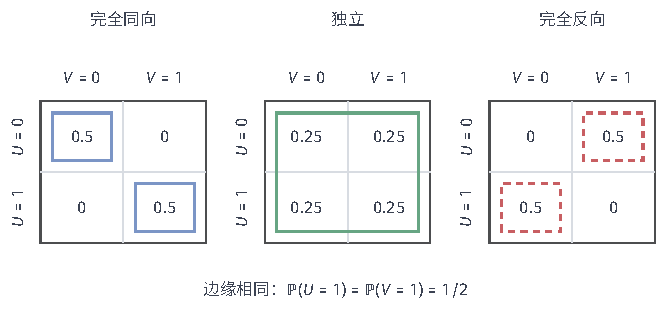
\includegraphics[width=\linewidth]{figures/01-mathematical-preliminaries/04-random-variables-distributions-and-causality/tikz/rv-dependence/figure.pdf}
  \caption{边缘质量相同的三个联合分布。格内数字是联合概率，各行各列的和始终为\(1/2\)；质量的位置改变协方差及和的分布。}
\label{fig:rv-dependence}
\end{figure}

\subsection{条件关系}
观测没有改变已经发生的读数，但改变了能够利用的信息。只想预测平均值时，条件期望足够；需要尾部概率、分位数或继续抽样时，则需要完整的条件分布。

\subsubsection{条件期望与信息投影}
\label{sec:rv-conditional-expectation}
% Baseline P:434-524
子\(\sigma\)代数\(\mathcal{G}\subseteq\mathcal{F}\)表示当前可用信息。预测值必须只使用这些信息，又应在每个可识别的分组内保持平均值。
\begin{definition}[观测生成的信息]
  \label{def:probability-generated-information}
若\(X:\Omega\to(\mathcal X,\mathcal A)\)是随机变量，记
\(\sigma(X)=\{X^{-1}(A):A\in\mathcal A\}\)。它是使\(X\)可测的最小\(\sigma\)代数，表示仅观察\(X\)能够区分的事件。多个观测生成的信息是包含它们全部可测逆像的最小\(\sigma\)代数。
\end{definition}
例如只观察分组编号，就不能在同一组内区分两个原始结果。写\(\mathbb E[Y\mid X]\)时，真正限制答案的信息是\(\sigma(X)\)，不是单个零概率事件\(\{X=x\}\)。
\begin{definition}[条件期望]
  \label{def:probability-conditional-expectation}
对\(X\in L^1(\mathbb P)\)，\term{条件期望}（conditional expectation）
\(\mathbb{E}[X\mid\mathcal{G}]\)是满足下列两项条件的可积随机变量\(Z\)：
\[ Z\text{ 对 }\mathcal{G}\text{ 可测},
  \qquad\int_A Z\,\mathrm{d}\mathbb{P}=\int_A X\,\mathrm{d}\mathbb{P}\quad(A\in\mathcal{G}). \]
\end{definition}
第一项要求答案只能使用\(\mathcal{G}\)中的信息，第二项要求它在每个可由当前信息识别的事件上保留\(X\)的平均
\scite{math-kallenberg2021probability}

\begin{theorem}[条件期望的存在与唯一性]
\label{thm:probability-conditional-expectation-existence}
若\(X\in L^1(\mathbb{P})\)，则\(\mathbb{E}[X\mid\mathcal{G}]\)存在，并在几乎处处意义下唯一。
\end{theorem}

\begin{proof}
先设\(X\geq0\)。在\((\Omega,\mathcal{G})\)上定义有限测度
\[ \nu(A)=\int_A X\,\mathrm{d}\mathbb{P}. \]
若\(\mathbb{P}(A)=0\)，则\(\nu(A)=0\)，所以\(\nu\ll\mathbb{P}|_{\mathcal{G}}\)。Radon--Nikodym定理给出非负、
\(\mathcal{G}\)-可测的\(Z\)，使\(\nu(A)=\int_A Z\,\mathrm{d}\mathbb{P}\)。对一般可积\(X\)，分别对
\(X^+\)与\(X^-\)使用这一构造并取差，即得存在性。

若\(Z_1,Z_2\)都满足定义，令\(D=Z_1-Z_2\)。对每个\(A\in\mathcal{G}\)，\(\int_A D\,\mathrm{d}\mathbb{P}=0\)。若
\(\mathbb{P}(D>0)>0\)，则某个集合\(A_k=\{D\geq1/k\}\)具有正概率，从而
\[ \int_{A_k}D\,\mathrm{d}\mathbb{P}
  \geq\frac{1}{k}\mathbb{P}(A_k)>0, \]
产生矛盾。因此\(D\leq0\)几乎处处。交换\(Z_1,Z_2\)可得\(D\geq0\)几乎处处，故二者几乎处处相等。
\end{proof}

积分的线性性与上述唯一性说明，条件期望也保持线性组合。
对非负变量，存在证明给出的Radon--Nikodym导数非负；
因此若\(X\leq Y\)且两者可积，对\(Y-X\)使用该构造便得到
\(\mathbb E[X\mid\mathcal G]\leq\mathbb E[Y\mid\mathcal G]\)几乎处处。
这就是条件期望的保序性。

若\(X\)本来就对\(\mathcal{G}\)可测，则\(\mathbb{E}[X\mid\mathcal{G}]=X\)几乎处处。若\(X\)与\(\mathcal{G}\)
独立，则条件期望等于常数\(\mathbb{E}[X]\)。若\(U\)有界且\(\mathcal{G}\)-可测，则
\begin{equation}
  \mathbb{E}[UX\mid\mathcal{G}]
  =
  U\mathbb{E}[X\mid\mathcal{G}].
  \label{eq:probability-taking-out-known-factor}
\end{equation}
可积的非有界\(U\)需要另外核对乘积可积性，不能仅凭“已知量可提出”略去条件。

有限分组把抽象定义化成逐组平均。若
\(A_1,\ldots,A_m\)是有限可测分割，
\(\mathcal{G}=\sigma(A_1,\ldots,A_m)\)，且每个
\(\mathbb{P}(A_j)>0\)，则
\begin{equation}
  \mathbb{E}[X\mid\mathcal{G}]
  =
  \sum_{j=1}^{m}
  \frac{\mathbb{E}[X\mathbb{I}_{A_j}]}
       {\mathbb{P}(A_j)}
  \mathbb{I}_{A_j}.
  \label{eq:probability-finite-partition-conditional-expectation}
\end{equation}
若某个分组概率为零，该组上的取值可以任意指定，因为条件期望只在几乎处处意义下唯一。

表~\ref{tab:probability-finite-partition-predictions}给出一个可复核例子。令
\(\mathcal{G}\)只能区分
\(A=\{\omega_1,\omega_2\}\)与
\(B=\{\omega_3,\omega_4\}\)。不使用分组信息时，最佳常数预测是
\(U_0=\mathbb{E}X=3.4\)；规则\(U_{\mathrm{grp}}\)虽然按组取值，却随意地在
\(A,B\)上分别预测\(0,4\)；条件均值\(m=\mathbb{E}[X\mid\mathcal{G}]\)则在两组
上分别等于\(1.2,5.6\)。
\begin{table}[htbp]
  \centering
  \small
  \begin{tabular}{ccccccc}
    \toprule
    结果 & 概率 & \(X\) & 分组 & \(U_0\) & \(U_{\mathrm{grp}}\) & \(m\) \\
    \midrule
    \(\omega_1\) & \(0.2\) & \(0\) & \(A\) & \(3.4\) & \(0\) & \(1.2\) \\
    \(\omega_2\) & \(0.3\) & \(2\) & \(A\) & \(3.4\) & \(0\) & \(1.2\) \\
    \(\omega_3\) & \(0.1\) & \(4\) & \(B\) & \(3.4\) & \(4\) & \(5.6\) \\
    \(\omega_4\) & \(0.4\) & \(6\) & \(B\) & \(3.4\) & \(4\) & \(5.6\) \\
    \midrule
    \multicolumn{4}{r}{平方风险\(\ \mathbb{E}[(X-U)^2]\)} &
    \(5.64\) & \(2.80\) & \(0.80\) \\
    \bottomrule
  \end{tabular}
  \caption{有限分组下的三类预测。分组信息使预测可以随\(A,B\)变化，但只有逐组条件
  均值在全部\(\mathcal{G}\)-可测平方可积预测中达到最小平方风险。}
  \label{tab:probability-finite-partition-predictions}
\end{table}
三列风险依次说明不同问题：获得分组信息可以优于无信息常数，但使用信息本身不保证已经
最优；式~\eqref{eq:probability-finite-partition-conditional-expectation}还要在每组
内选择正确的条件平均。
% Baseline P:532-625
\begin{theorem}[塔式性质]
\label{thm:probability-tower-property}
若\(X\in L^1\)，且\(\mathcal{H}\subseteq\mathcal{G}\subseteq\mathcal{F}\)，则
\[ \mathbb{E}\bigl[\mathbb{E}[X\mid\mathcal{G}]
  \mid\mathcal{H}\bigr]=\mathbb{E}[X\mid\mathcal{H}] \]
几乎处处成立。
\end{theorem}

\begin{proof}
左侧对\(\mathcal{H}\)可测。对任意\(A\in\mathcal{H}\)，由于\(A\in\mathcal{G}\)，条件期望定义给出
\[
  \int_A
  \mathbb{E}\bigl[\mathbb{E}[X\mid\mathcal{G}]
  \mid\mathcal{H}\bigr]\,\mathrm{d}\mathbb{P}
  =
  \int_A\mathbb{E}[X\mid\mathcal{G}]\,\mathrm{d}\mathbb{P}
  =
  \int_A X\,\mathrm{d}\mathbb{P}.
\]
左侧因而满足\(X\)关于\(\mathcal{H}\)的条件期望定义，唯一性给出结论。
\end{proof}

取\(\mathcal{H}=\{\varnothing,\Omega\}\)，便得到\term{全期望公式}（law of total expectation）
\begin{equation}
  \mathbb{E}\bigl[\mathbb{E}[X\mid\mathcal{G}]\bigr]
  =
  \mathbb{E}[X].
  \label{eq:probability-total-expectation}
\end{equation}
这说明条件化改变可用信息，却不改变再平均后的总体均值。

\par\medskip\noindent\textbf{全方差分解}\quad
设\(X\in L^2\)，记\(m=\mathbb{E}[X\mid\mathcal{G}]\)。分解
\[ X-\mathbb{E}X=(X-m)+(m-\mathbb{E}X). \]
在展开平方前，需要先确认条件均值仍然二阶可积。
对每个有理数\(q\)，条件期望的线性性与保序性给出
\[
 \mathbb E[X^2\mid\mathcal G]-2qm+q^2
 =\mathbb E[(X-q)^2\mid\mathcal G]\geq0.
\]
有理数只有可数个，可以在同一个满测集上同时使用这些不等式。
由于\(\sup_{q\in\mathbb Q}(2qm-q^2)=m^2\)，得到
\[
  |m|^2
  \leq
  \mathbb{E}[X^2\mid\mathcal{G}].
\]
再取期望并使用全期望公式，得到
\[
  \mathbb{E}[m^2]\leq\mathbb{E}[X^2]<\infty.
\]
因此\(m\in L^2\)，上面分解中的两项都二阶可积，其乘积由Cauchy--Schwarz不等式保证可积。又因为第二项对
\(\mathcal{G}\)可测，而\(\mathbb{E}[X-m\mid\mathcal{G}]=0\)，所以交叉项期望为
\[ \mathbb{E}\bigl[(X-m)(m-\mathbb{E}X)\bigr]
  =\mathbb{E}\left[(m-\mathbb{E}X)\mathbb{E}[X-m\mid\mathcal{G}]\right]=0. \]
展开平方得到\term{全方差公式}（law of total variance）
\begin{equation}
  \operatorname{Var}(X)
  =
  \mathbb{E}\bigl[\operatorname{Var}(X\mid\mathcal{G})\bigr]
  +
  \operatorname{Var}\bigl(\mathbb{E}[X\mid\mathcal{G}]\bigr),
  \label{eq:probability-total-variance}
\end{equation}
其中
\[ \operatorname{Var}(X\mid\mathcal{G})
  =\mathbb{E}\bigl[(X-m)^2\mid\mathcal{G}\bigr]. \]
第一项是获得\(\mathcal{G}\)后仍无法解释的平均波动，第二项是不同信息状态之间的可解释波动。

刚才的平方界是条件Jensen不等式（conditional Jensen inequality）的一个实例。
一般地，若\(\phi:\mathbb R\to\mathbb R\)为凸函数，\(X\)与\(\phi(X)\)都可积，则
\[
 \phi\bigl(\mathbb E[X\mid\mathcal G]\bigr)
 \leq\mathbb E[\phi(X)\mid\mathcal G]\quad\text{几乎处处}.
\]
其依据仍是仿射下界：在每个有理点选取一条支撑线
\(a_qx+b_q\leq\phi(x)\)，凸函数的连续性保证这些支撑线的上确界等于\(\phi\)。
对每条线取条件期望，得到
\(a_qm+b_q\leq\mathbb E[\phi(X)\mid\mathcal G]\)，
再在共同满测集上取可数上确界即可。
对有限维随机向量，把支撑线换成仿射支撑超平面，论证相同；
凸函数只定义在凸域上时，还需条件均值属于该域，并核对相关量的可积性。
取不含额外信息的平凡条件，便得到通常的积分Jensen不等式。

\par\medskip\noindent\textbf{条件期望的平方损失最优性}\quad
\begin{theorem}[条件均值的平方损失最优性]
\label{thm:probability-conditional-mean-l2-projection}
设\(X\in L^2(\mathbb{P})\)。在所有\(\mathcal{G}\)-可测且二阶可积的随机变量\(U\)中，
\[ m=\mathbb{E}[X\mid\mathcal{G}] \]
唯一地在几乎处处意义下最小化\(\mathbb{E}[(X-U)^2]\)。
\end{theorem}

\begin{proof}
\(L^2(\mathcal{G})\)是\(L^2(\mathcal{F})\)的闭线性子空间，上文直接证明的条件平方界已经说明
\(m\in L^2(\mathcal{G})\)。对每个\(U\in L^2(\mathcal{G})\)，Cauchy--Schwarz不等式保证
\((X-m)U\)可积，因而可以提出已知因子并使用塔式性质，得到
\[ \mathbb{E}[(X-m)U]
  =\mathbb{E}\left[U\mathbb{E}[X-m\mid\mathcal{G}]\right]=0. \]
所以\(X-m\)与整个\(L^2(\mathcal{G})\)正交。定理~\ref{thm:functional-hilbert-projection}说明\(m\)是\(X\)到该闭子空间的正交投影。也可直接展开
\begin{equation}
  \mathbb{E}[(X-U)^2]
  =
  \mathbb{E}[(X-m)^2]
  +
  \mathbb{E}[(m-U)^2],
  \label{eq:probability-pythagorean-prediction}
\end{equation}
交叉项因正交性消失。第二项非负，且仅当\(U=m\)几乎处处时为零。
\end{proof}

条件期望的存在只需要\(X\in L^1\)，这时它由Radon--Nikodym导数给出。“正交投影”和平方损失最优性则需要\(X\in L^2\)。若二阶矩无限，条件期望仍可能
存在，但不能使用Hilbert空间几何或有限平方风险。


\subsubsection{条件分布与概率核}
\label{sec:rv-conditional-distribution}
% Baseline P:370-413
当条件变量连续时，事件\(\{X=x\}\)常有零概率，直接相除不再可行。需要把“每个条件值对应一个分布”组织成能继续积分的对象。
\begin{definition}[概率核]
  \label{def:probability-kernel}
  给定可测空间\((\mathcal X,\mathcal A)\)、\((\mathcal Y,\mathcal B)\)，\term{概率核}（probability kernel）是映射
  \[ K:\mathcal X\times\mathcal B\to[0,1], \]
  满足：对每个\(x\in\mathcal X\)，\(K(x,\cdot)\)是\((\mathcal Y,\mathcal B)\)上的概率测度；对每个\(B\in\mathcal B\)，\(x\mapsto K(x,B)\)是\(\mathcal A\)-可测函数。
\end{definition}
第一项保证每个条件值给出合法分布，
第二项保证再对\(X\)积分是合法运算。

可测并不等于连续。例如取\(X\sim\mathcal N(0,1)\)、\(Y=\mathbb I\{X\geq0\}\)，则\(K(x,\{1\})=\mathbb I\{x\geq0\}\)是合法概率核在事件\(\{1\}\)上的取值，却在\(x=0\)处跳变。条件值\(x\)可以连续取值，条件分布随\(x\)变化仍可不连续。

\begin{definition}[正则条件分布]
  \label{def:probability-regular-conditional-distribution}
若概率核\(K\)对所有\(A\in\mathcal A\)、\(B\in\mathcal B\)满足
\begin{equation}
  \mathbb{P}(X\in A,Y\in B)
  =
  \int_A K(x,B)\,\mathbb{P}_X(\mathrm{d}x),
  \label{eq:probability-regular-conditional-kernel}
\end{equation}
就把\(K(x,\cdot)\)称为\(Y\)给定\(X=x\)的一个\term{正则条件分布}（regular conditional distribution）。
\end{definition}
对每个固定可测集\(B\)，两个版本的\(K(x,B)\)在\(\mathbb P_X\)-几乎处处意义下相同；若\(\mathcal Y\)是下面的标准Borel空间，还可选取一个共同零测集，使其外的条件概率测度相同。零概率条件点上的取值通常不能由联合分布唯一决定。

\begin{example}[条件分布版本可以怎样不同]
\label{ex:probability-conditional-kernel-versions}
设\(X\sim\operatorname{Unif}[0,1]\)，并令\(Y=X\)。给定\(x\)，取
\(K(x,\cdot)=\delta_x\)，即全部条件概率质量集中在\(y=x\)。对任意Borel集\(A,B\)，
\[
 \begin{aligned}
 \mathbb P(X\in A,Y\in B)
 &=\mathbb P(X\in A\cap B)\\
 &=\int_A\mathbb I_B(x)\,\mathbb P_X(\mathrm dx)
  =\int_A K(x,B)\,\mathbb P_X(\mathrm dx).
 \end{aligned}
\]
因此\(K\)是一个正则条件分布。现在只在\(x=1/2\)处把\(\delta_x\)改成\(\delta_0\)，
其余点不变，得到另一个可测概率核\(\widetilde K\)。由于
\(\mathbb P_X(\{1/2\})=0\)，上述积分不变，\(\widetilde K\)也是同一联合分布的条件版本。
两个版本在共同零测集\(\{1/2\}\)之外给出完全相同的概率测度。

这里每个单点\(\{x\}\)都有零概率，却不能因此在所有点上任意改值：不可数个零概率
单点的并集可以具有正概率。若把全部\(K(x,\cdot)\)都改成\(\delta_0\)，它就不再
重建\(Y=X\)的联合分布。“几乎处处唯一”约束的是两个完整条件核可以在哪一整个
集合上不同，而不是逐点检查后随意拼接答案。

此例的联合分布全部集中在对角线\(y=x\)上。对角线的二维Lebesgue测度为零，
所以不存在普通二维联合密度；正则条件分布仍然存在。条件核因而比密度比值公式更一般。
\end{example}

\par\medskip\noindent\textbf{正则条件分布的存在条件}\quad
逐个条件事件的概率能够定义，并不保证它们能拼成一个共同的概率核。下面的可测空间条件为这种拼接提供保证。
\begin{definition}[Polish空间]
  \label{def:probability-polish-space}
从一个度量空间出发，允许更换距离但保持同一族开集。
若能选到完备且可分的距离，就称这个空间为Polish空间。
保持开集不变也保持相同的连续映射，这就是“距离与原拓扑兼容”的含义。
可分表示含有可数稠密子集；完备性表示所选距离下每个Cauchy序列都在空间内收敛。
\end{definition}
欧氏空间就是一个例子。这里要求存在合适的距离，不要求最初写下的那个距离已经完备。
例如\((0,1)\)的通常距离不完备，但连续双射\(x\mapsto\log(x/(1-x))\)
把它映到实轴，逆也连续；拉回实轴距离得到
\[
 d'(x,y)=\left|\log\frac{x}{1-x}-\log\frac{y}{1-y}\right|.
\]
这个距离保持原开集，并把该区间变为与实轴等距的完备可分空间。
标准Borel空间进一步只保留这样的可测结构。
\begin{definition}[标准Borel空间]
  \label{def:probability-standard-borel-space}
  可测空间称为\term{标准Borel空间}（standard Borel space），若它与某个完备可分度量空间的Borel子集可测同构，即存在双射，且该双射及其逆映射都可测。
\end{definition}
这里不要求展示出来的Borel子集在继承距离下完备。
若\(X\)与\(Y\)的状态空间都是标准Borel空间，则上述正则条件分布存在。实数空间、欧氏空间、可数集合以及配备适当Borel结构的常见可分函数空间都属于这一范围。

这一存在结论依赖可数生成结构与上一小节的条件期望：需要把逐个事件上的条件平均整理成同一个概率核。

在完全一般的可测空间上，正则条件分布可能不存在。此时条件期望仍可相对于子\(\sigma\)代数定义，但不能未经说明就把它写成每个点\(x\)上的条件密度。后续模型
通常工作在标准Borel空间中；使用\(p(y\mid x)\)时，应同时确认密度所依赖的参考测度及其适用的几乎处处范围。

% Baseline P:526-528
构造思路可以从可数生成族看清。先在\(\mathcal{Y}\)的一个可数、能区分概率测度的集合族上，对每个\(B\)构造
\(\mathbb{P}(Y\in B\mid\sigma(X))\)；再选取这些条件期望关于\(X\)的可测版本。在去掉一个共同零测集后，这些数值满足有限可加性和连续性，扩张定理把它们唯一延拓为
\(\mathcal{Y}\)上的概率测度。标准Borel结构提供的可数性和可分性，正是把逐个事件的版本整理成同一个概率核所需的条件。
% Baseline P:335-366
当\(p_X(x)>0\)时，离散条件质量定义为
\[ p_{Y\mid X}(y\mid x)
  =\frac{p_{X,Y}(x,y)}{p_X(x)}. \]
因此有乘法公式
\[ p_{X,Y}(x,y)=p_X(x)p_{Y\mid X}(y\mid x). \]
若\(p_Y(y)>0\)，把联合质量按另一顺序分解便得到Bayes公式
\begin{equation}
  p_{X\mid Y}(x\mid y)
  =
  \frac{p_{Y\mid X}(y\mid x)p_X(x)}
       {\sum_{x'}p_{Y\mid X}(y\mid x')p_X(x')}.
  \label{eq:probability-discrete-bayes}
\end{equation}
分母是观测\(y\)的边缘概率，既负责归一化，也要求观测并非零概率事件。

连续密度公式是同一分解的特例。若\((X,Y)\)相对于乘积参考测度有联合密度
\(f_{X,Y}\)，且\(0<f_X(x)<\infty\)，则
\[
  f_{Y\mid X}(y\mid x)
  =\frac{f_{X,Y}(x,y)}{f_X(x)}
\]
非负并对\(y\)积分为\(1\)。它满足
\(f_{X,Y}(x,y)=f_X(x)f_{Y\mid X}(y\mid x)\)。在
\(f_X(x)=0\)或\(f_X(x)=\infty\)的点上，不能使用这个比值；这些点构成\(\mathbb P_X\)-零测集。条件核在该零测集上可统一指定一个固定概率测度，而不改变联合分布。这里选用由联合密度积分得到的边缘密度版本；任意修改过的密度版本也只能保证相应等式几乎处处成立。

\begin{example}[有限候选经过带噪观测更新]
\label{ex:probability-finite-candidate-bayes}
设信号只可能是\(\Theta\in\{-1,1\}\)，先验概率均为\(1/2\)。传感器以概率\(0.8\)报告正确符号。观测\(Y=1\)后，
\[ \mathbb{P}(\Theta=1\mid Y=1)
  =\frac{0.8\times0.5}{0.8\times0.5+0.2\times0.5}=0.8. \]
观测并未把候选集合改成一个确定点，而是改变了两个候选的相对权重。若某个观测在所有
候选下概率都为零，公式分母为零，条件分布不能靠这个比值定义。
\end{example}
% Baseline P:1130-1183
设\(\bm X\sim\mathcal N(\bm\mu,\bm\Sigma)\)是联合高斯向量。把向量、均值及协方差按相同坐标分块，其中
\[
  \bm{X}=
  \begin{bmatrix}\bm{X}_1\\\bm{X}_2\end{bmatrix},
  \qquad
  \bm{\Sigma}=
  \begin{bmatrix}
    \bm{\Sigma}_{11}&\bm{\Sigma}_{12}\\
    \bm{\Sigma}_{21}&\bm{\Sigma}_{22}
  \end{bmatrix},
\]
边缘\(\bm{X}_1\)仍为\(\mathcal{N}(\bm{\mu}_1,\bm{\Sigma}_{11})\)。若\(\bm{\Sigma}_{22}\)可逆，配方或第~\ref{chap:matrix-analysis}章的Schur补运算给出
\begin{align}
  \bm{X}_1\mid\bm{X}_2=\bm{x}_2
  \sim\mathcal{N}\bigl(
  &\bm{\mu}_1+
  \bm{\Sigma}_{12}\bm{\Sigma}_{22}^{-1}
  (\bm{x}_2-\bm{\mu}_2),\notag\\
  &\bm{\Sigma}_{11}
  -\bm{\Sigma}_{12}\bm{\Sigma}_{22}^{-1}
  \bm{\Sigma}_{21}
  \bigr).
  \label{eq:probability-conditional-gaussian}
\end{align}
条件均值是观测的仿射函数，条件协方差不依赖具体观测值。若分块协方差奇异，需要使用广义逆并在支持子空间上解释条件分布，不能直接套用逆矩阵公式。

式~\eqref{eq:probability-conditional-gaussian}也可由一个独立残差推导。令
\[
  \bm{R}
  =\bm{X}_1-\bm{\mu}_1
   -\bm{\Sigma}_{12}\bm{\Sigma}_{22}^{-1}
    (\bm{X}_2-\bm{\mu}_2).
\]
直接计算得到
\(\operatorname{Cov}(\bm{R},\bm{X}_2)=\bm{0}\)，且
\[
  \operatorname{Cov}(\bm{R})
  =\bm{\Sigma}_{11}
   -\bm{\Sigma}_{12}\bm{\Sigma}_{22}^{-1}\bm{\Sigma}_{21}.
\]
\((\bm{R},\bm{X}_2)\)是联合高斯向量，零交叉协方差因而推出独立。给定
\(\bm{X}_2=\bm{x}_2\)后，\(\bm{R}\)的分布不变，把定义式移项便得到条件均值与条件协方差。

例如令信号\(S\sim\mathcal{N}(0,4)\)，观测
\(Y=S+\varepsilon\)，其中\(\varepsilon\sim\mathcal{N}(0,1)\)且与\(S\)独立。于是
\[
  \operatorname{Cov}
  \begin{pmatrix}S\\Y\end{pmatrix}
  =
  \begin{bmatrix}4&4\\4&5\end{bmatrix},
  \qquad
  S\mid Y=y\sim\mathcal{N}\left(\frac45y,\frac45\right).
\]
观测到\(y=2\)时，条件均值为\(1.6\)，条件方差由先验的\(4\)降到\(0.8\)。第~\ref{chap:dynamical-systems-and-state-estimation}章的线性高斯滤波会逐时重复这一块条件计算，但还需要动态与观测独立性假设。
% Baseline T:970-975
总体分位数来自混合不同输入后的边缘分布；若不同\(x\)对应不同位置或尾部，还需要按输入报告条件分位数。
\begin{definition}[条件分位数]
  \label{def:statistics-conditional-quantile}
给定\(Y\)关于\(X=x\)的正则条件分布，记\(F_x(y)=\mathbb P(Y\leq y\mid X=x)\)。对\(0<q<1\)，下条件\(q\)分位数为\(F_x^{-1}(q)=\inf\{y:F_x(y)\geq q\}\)；完整条件分位数集合为\(\{a:F_x(a^-)\leq q\leq F_x(a)\}\)。这些对象随条件分布版本确定，并按\(P_X\)-几乎处处意义理解。
\end{definition}
条件分位数是已知条件分布的特征；从数据估计整条条件分位函数的方法见第~\ref{sec:statistics-nonparametric-missing}节。

\subsection{独立关系}
\label{sec:probability-moments-independence}
% Baseline P:720-821

\par\medskip\noindent\textbf{独立、不相关与非线性依赖}\quad
若随机变量\(X,Y\)满足
\[ \mathbb{P}(X\in A,Y\in B)
  =\mathbb{P}(X\in A)\mathbb{P}(Y\in B) \]
对所有Borel集合\(A,B\)成立，就称二者\term{独立}（independent）。独立意味着所有可积可分函数都满足
\(\mathbb{E}[g(X)h(Y)]=\mathbb{E}[g(X)]\mathbb{E}[h(Y)]\)。
证明从指示函数开始：独立性正好说明结论对
\(g=\mathbb{I}_A\)、\(h=\mathbb{I}_B\)成立。线性性把它推广到简单函数，随后分别用单调收敛处理非负函数，再分解正负部分处理乘积可积的实值函数。这里必须要求相关积分有定义，不能把两个发散期望形式相乘。

协方差只检查中心化变量的一次乘积。令\(X\)在\([-1,1]\)上均匀分布，并取\(Y=X^2\)。对称性给出
\[ \operatorname{Cov}(X,Y)
  =\mathbb{E}[X^3]-\mathbb{E}[X]\mathbb{E}[X^2]=0, \]
但\(Y\)由\(X\)完全决定；知道\(X\)便能确定\(Y\)，所以二者不独立。零协方差只排除了线性二阶关联。

\par\medskip\noindent\textbf{条件独立及其运算规则}\quad
\begin{definition}[条件独立]
  \label{def:probability-conditional-independence}
  给定随机变量\(X,Y,Z\)，若对\(X,Y\)取值空间中的所有可测集合\(A,B\)，
\[ \mathbb{P}(X\in A,Y\in B\mid Z)
  =\mathbb{P}(X\in A\mid Z)\mathbb{P}(Y\in B\mid Z) \]
几乎处处成立，就称\(X\)与\(Y\)在给定\(Z\)时条件独立，记作
\(X\perp Y\mid Z\)。
\end{definition}
它表示\(Z\)已知以后，\(X\)不再提供关于\(Y\)的额外分布信息；这不意味着去掉\(Z\)后仍独立。

条件独立满足以下常用规则：
\[
\begin{aligned}
  X\perp Y\mid Z
  &\Longrightarrow Y\perp X\mid Z
  &&\text{（对称性）},\\
  X\perp(Y,W)\mid Z
  &\Longrightarrow X\perp Y\mid Z
  &&\text{（分解）},\\
  X\perp(Y,W)\mid Z
  &\Longrightarrow X\perp Y\mid Z,W
  &&\text{（弱并）},\\
  X\perp Y\mid Z,\quad X\perp W\mid Y,Z
  &\Longrightarrow X\perp(Y,W)\mid Z
  &&\text{（收缩）}.
\end{aligned}
\]
这些规则可由条件核的乘积分解逐项验证。交性质
\[ X\perp Y\mid Z,W,\quad
  X\perp W\mid Z,Y\Longrightarrow X\perp(Y,W)\mid Z \]
并非无条件成立；严格为正的有限离散联合质量是一个常用充分条件。若分布把质量集中在
低维约束上，零概率组合会阻断所需的消元步骤。

\begin{lemma}[严格正离散分布的交性质]
  \label{lem:probability-positive-intersection}
  设$I$为有限索引集，每个$i\in I$对应取值于有限非空状态空间$\mathcal{X}_i$的随机变量$X_i$。令$p$为$\bm{X}=(X_i)_{i\in I}$在乘积状态空间$\mathcal{X}=\prod_{i\in I}\mathcal{X}_i$上的联合质量函数，且$p(\bm{x})>0$对所有$\bm{x}\in\mathcal{X}$成立。对两两不交的索引集$A,B,C,D\subseteq I$，若
  \[
    \bm{X}_A\perp\bm{X}_B\mid(\bm{X}_C,\bm{X}_D),
    \qquad
    \bm{X}_A\perp\bm{X}_D\mid(\bm{X}_C,\bm{X}_B),
  \]
  则
  \[
    \bm{X}_A\perp(\bm{X}_B,\bm{X}_D)\mid\bm{X}_C.
  \]
\end{lemma}

\begin{proof}
严格正性保证以下每个条件概率都有定义。对任意取值$\bm{a},\bm{b},\bm{c},\bm{d}$，两个前提分别给出
\[
  p(\bm{a}\mid\bm{b},\bm{c},\bm{d})
  =p(\bm{a}\mid\bm{c},\bm{d}),
  \qquad
  p(\bm{a}\mid\bm{b},\bm{c},\bm{d})
  =p(\bm{a}\mid\bm{b},\bm{c}).
\]
因此$p(\bm{a}\mid\bm{c},\bm{d})=p(\bm{a}\mid\bm{b},\bm{c})$对每个$\bm{b},\bm{d}$成立。固定任意基准值$\bm{b}^{\circ}$，右侧等于$q(\bm{a},\bm{c})=p(\bm{a}\mid\bm{b}^{\circ},\bm{c})$，不再依赖$\bm{b}$或$\bm{d}$。对$(\bm{b},\bm{d})$关于$p(\bm{b},\bm{d}\mid\bm{c})$求和可得$q(\bm{a},\bm{c})=p(\bm{a}\mid\bm{c})$，故$p(\bm{a}\mid\bm{b},\bm{c},\bm{d})=p(\bm{a}\mid\bm{c})$，这正是所需的条件独立性。
\end{proof}
严格正性使上面证明能在固定\(\bm c\)后独立改变\(\bm b\)和\(\bm d\)。若只支持部分组合，这一步会失败。一个反例是\(X=Y=W=B\)，其中\(B\)为非退化Bernoulli变量，\(Z\)取常数。给定\(W\)后\(X,Y\)都确定，所以\(X\perp Y\mid W\)；给定\(Y\)后也有\(X\perp W\mid Y\)。但\(X\)与\((Y,W)\)显然不独立，因为后者直接给出\(X\)。两个条件独立前提因而不能在这类带零概率配置的分布上推出交性质。

以分解和收缩为例可以看清这些规则使用了什么。若
\(X\perp(Y,W)\mid Z\)，则对任意可测集合\(A,B,C\)，条件核满足
\[
  K_{X,Y,W\mid Z}(A,B,C\mid z)
  =K_{X\mid Z}(A\mid z)K_{Y,W\mid Z}(B,C\mid z).
\]
令\(C\)取全集便得到
\(K_{X,Y\mid Z}=K_{X\mid Z}K_{Y\mid Z}\)，这就是分解规则。对收缩规则，假设
\[
  K_{X,Y\mid Z}=K_{X\mid Z}K_{Y\mid Z},
  \qquad
  K_{X,W\mid Y,Z}=K_{X\mid Y,Z}K_{W\mid Y,Z}.
\]
第一个条件还给出
\(K_{X\mid Y,Z}=K_{X\mid Z}\)的一个版本。沿条件乘法公式相乘可得
\[
  K_{X,Y,W\mid Z}
  =K_{X\mid Z}K_{Y\mid Z}K_{W\mid Y,Z}
  =K_{X\mid Z}K_{Y,W\mid Z},
\]
即\(X\perp(Y,W)\mid Z\)。所有等式都按相应条件变量分布的几乎处处意义理解。概率图模型部分会在这些概率规则之上另加图分离语义；图上没有边本身并不是这里定义的条件独立证明。

多元高斯分布是一个特殊情形：联合高斯随机向量的两个子向量若协方差为零，则它们独立；条件高斯中的条件协方差为零也对应条件独立。这个结论依赖高斯
密度由一、二阶矩完全确定，不能推广到一般分布。

\subsection{可交换关系}
\label{sec:rv-exchangeability}
% Baseline P:2279-2289
\begin{definition}[可交换随机变量]
  \label{def:probability-exchangeability}
随机变量\(Z_1,\ldots,Z_m\)若对每个排列\(\pi\)都有
\[ (Z_1,\ldots,Z_m)
  \overset{\mathrm{d}}{=}(Z_{\pi(1)},\ldots,Z_{\pi(m)}), \]
就称它们\term{可交换}（exchangeable）。
\end{definition}
独立同分布蕴含可交换，但反向不成立。
例如先抽取随机概率\(\Theta\)，再条件于\(\Theta\)独立生成Bernoulli观测；边缘上这些观测可交换，却因共享\(\Theta\)而相关。

可交换性不提供样本平均的独立乘积结构，因而不能直接代入Hoeffding证明。
它提供的是标签位置的对称性：若评分规则在重排观测时只把分数作同样的重排，
并且分数几乎必然没有并列，则每个分数占据每个秩的概率都是\(1/m\)。
因为所有标签机会相同，而每个秩又恰由一个标签占据，概率总和必须为\(1\)。
有并列时，可为每个分数附加一个服从\(\operatorname{Unif}(0,1)\)的随机数，
这些随机数相互独立，并且独立于全部分数。
按“先分数、相同时再随机数”排序；这保留对称性并消除并列，从而恢复均匀秩。
若采用不随机化的并列规则，则通常只能得到相应的保守概率界。
后面的共形预测会明确区分这两种处理，使用它们各自的有限样本结论。
例如共享参数\(\Theta\sim\operatorname{Beta}(2,2)\)，给定\(\Theta\)后
\(X_i\)独立服从\(\operatorname{Bernoulli}(\Theta)\)。每个边缘的成功率为\(1/2\)，但对\(i\ne j\)，塔式性质给出
\[
\operatorname{Cov}(X_i,X_j)
=\mathbb E[\Theta^2]-(\mathbb E\Theta)^2
=\operatorname{Var}(\Theta)=\frac1{20}.
\]
因此\(\mathbb P(X_1=X_2=1)=0.3\)，大于独立情况下的\(0.25\)。
共享背景使一串成功更常一起出现，却没有偏爱某个观测编号。有限可交换性本身不保证一定存在这样的独立混合表示；本例是可交换依赖的一种构造。

\section{随机变量的运算与变换}
\label{sec:rv-transformations}
\label{sec:probability-random-vectors-transformations}
两台传感器的读数相加，是改变取值规则；给定设备状态后再抽取噪声，是加入条件随机生成；保持读数规则却改变设备状态的抽取概率，是改变概率权重。三种操作都能改变输出分布，计算时应先辨明改变的是哪一部分。

\subsection{确定函数下的变换与组合}
“确定”指作用规则确定，而不是输出不随机。输入一旦实现，函数输出才随之唯一确定。

\subsubsection{分布变换的通用规则}
\label{sec:rv-pushforward}
若\(X\)取值于\((E,\mathcal E)\)，\(g:E\to F\)可测，则
\(Y=g(X)\)的分布是\(P_Y=g_\#P_X\)，即
\[
P_Y(B)=P_X(g^{-1}(B)),\qquad
\mathbb E h(Y)=\int_E h(g(x))\,P_X(\mathrm dx)
\]
对非负可测\(h\)或可积\(h\)成立。这个规则不要求密度，也不要求\(g\)可逆。
% Baseline P:1187-1202
设\(\bm{Y}=g(\bm{X})\)，其中\(g:\mathcal{X}\to\mathcal{Y}\)为可微双射，逆映射也可微。第~\ref{chap:mathematical-analysis}章的换元公式给出
\begin{equation}
  f_{\bm{Y}}(\bm{y})
  =
  f_{\bm{X}}\bigl(g^{-1}(\bm{y})\bigr)
  \left|
    \det\bm{J}_{g^{-1}}(\bm{y})
  \right|.
  \label{eq:probability-density-change-variables}
\end{equation}
Jacobian矩阵的行列式补偿局部体积变化。只把\(x=g^{-1}(y)\)代入原密度而漏掉该因子，所得函数通常不能积分为\(1\)。

若映射不是一一对应，需要对所有逆像分支求和。例如\(Y=X^2\)且\(X\)有密度时，对\(y>0\)，
\[ f_Y(y)
  =\frac{f_X(\sqrt{y})+f_X(-\sqrt{y})}{2\sqrt{y}}. \]
若输出维数低于输入维数，分布可能集中到低维集合，此时不能期待相对于原维度Lebesgue测度的普通密度。
非方阵Jacobian不能直接取行列式换元。若
\((X_1,X_2)\)在单位正方形上均匀分布，投影\(g(x_1,x_2)=x_1\)降到一维，输出仍有一维密度\(1_{[0,1]}\)，由对\(x_2\)积分得到。相反，嵌入\(h(x)=(x,x)\)把一维变量放入二维，像落在直线上，没有二维Lebesgue密度。应比较输出支持与输出空间的维数，而不能把“降维”直接等同于“没有密度”。

\subsubsection{数值变量的组合运算}
\label{sec:rv-combinations}
可积变量的和满足\(\mathbb E(X+Y)=\mathbb EX+\mathbb EY\)，不需要独立；
二阶可积时
\[
\operatorname{Var}(aX+bY)
=a^2\operatorname{Var}(X)+b^2\operatorname{Var}(Y)
 +2ab\operatorname{Cov}(X,Y).
\]
图~\ref{fig:rv-dependence}中三个和的方差依次为\(1,1/2,0\)。相同边缘并没有给出相同的累计波动。若只知两个变量可积，乘积未必可积；二阶可积则由Cauchy--Schwarz保证乘积可积。比值还须确保分母非零，且另查比值的矩。

若\(X,Y\)具有联合密度\(f_{X,Y}\)，换元与边缘化给出
\[
\begin{aligned}
f_{X+Y}(s)&=\int_{\mathbb R}f_{X,Y}(x,s-x)\,\mathrm dx,\\
f_{XY}(z)&=\int_{\mathbb R\setminus\{0\}}
 f_{X,Y}(x,z/x)\frac{\mathrm dx}{|x|},\\
f_{X/Y}(r)&=\int_{\mathbb R}|y|f_{X,Y}(ry,y)\,\mathrm dy.
\end{aligned}
\]
后两式的Jacobian因子分别为\(1/|x|\)和\(|y|\)。独立时联合密度可分解，和的密度便是卷积\(f_X*f_Y\)；离散和相应使用
\(\mathbb P(X+Y=s)=\sum_x\mathbb P(X=x)\mathbb P(Y=s-x)\)。
例如独立标准高斯之比\(R=X/Y\)满足
\[
f_R(r)=\frac1{2\pi}\int_{\mathbb R}|y|
 e^{-(1+r^2)y^2/2}\,\mathrm dy
=\frac1{\pi(1+r^2)}.
\]
这是标准Cauchy密度，\(\mathbb E|R|=\infty\)。分子分母都拥有全部矩，也不保证比值有均值。

独立性还把变换函数化为乘积：
\[
\varphi_{X+Y}(t)=\mathbb E(e^{\mathrm itX}e^{\mathrm itY})
=\varphi_X(t)\varphi_Y(t).
\]
在矩母函数共同有限的邻域，同样有
\(M_{X+Y}=M_XM_Y\)、\(K_{X+Y}=K_X+K_Y\)。向量的独立坐标使联合累积量生成函数按坐标相加，所有跨坐标累积量为零；在原点邻域解析的条件下，反向由变换函数唯一性得到。高阶累积量可识别协方差未反映的非高斯依赖，纯高斯的三阶及以上累积量则为零。
独立Poisson变量的矩母函数为
\(\exp\{\lambda(e^t-1)\}\)，相乘后参数相加；独立标准高斯平方的Gamma矩母函数相乘，则得到前面定义的卡方分布。

对向量，令\(\bm Y=\bm A\bm X+\bm b\)，相应矩存在时
\[
\mathbb E\bm Y=\bm A\bm\mu+\bm b,\quad
\operatorname{Cov}(\bm Y)=\bm A\bm\Sigma\bm A^\top,\quad
\operatorname{Cov}(\bm A\bm X,\bm B\bm X)=\bm A\bm\Sigma\bm B^\top.
\]
前两条不要求高斯性。若\(\bm X\)联合高斯，则任意线性组合仍高斯，因而
\(\bm Y\sim\mathcal N(\bm A\bm\mu+\bm b,\bm A\bm\Sigma\bm A^\top)\)，即使\(\bm A\)不满秩也成立，但不能因此写出非退化密度。

协方差变换式也说明了白化（whitening）的含义：对中心化向量作线性变换，使协方差成为单位阵。若\(\bm\Sigma\succ\bm0\)，可取
\(\bm Y=\bm\Sigma^{-1/2}(\bm X-\bm\mu)\)；此后任何正交旋转\(\bm Q\bm Y\)仍有单位协方差，因为\(\bm Q\bm I\bm Q^\top=\bm I\)。
因此二阶统计量无法继续辨认这些旋转方向。独立成分分析（independent component analysis, ICA）希望从若干源信号的线性混合观测中，辨认相互独立的源。
源具有适当的非高斯性时，高阶统计量可以提供白化后仍缺少的方向信息；纯高斯的三阶及以上累积量全为零，不能承担这一任务。这里说明的是高阶信息的用途，并不保证任意三阶、四阶量都足以唯一识别源。

排序也是函数变换。若\(X_1,\ldots,X_n\)独立同分布，分布函数为\(F\)，则
\[
\mathbb P(\max_iX_i\leq x)=F(x)^n,\quad
\mathbb P(\min_iX_i>x)=(1-F(x))^n,
\]
\[
\mathbb P(X_{(k)}\leq x)
=\sum_{j=k}^n\binom njF(x)^j(1-F(x))^{n-j}.
\]
这里把“第\(k\)小不超过\(x\)”改写成至少\(k\)个输入不超过\(x\)，所以出现二项计数。
% Baseline T:963-968
对次序统计量\(Y_{(1)}\leq\cdots\leq Y_{(n)}\)，经验分位数由相应秩位置给出。
若\(Y_1,\ldots,Y_n\)是来自连续分布\(F\)的独立同分布样本，则
\(F(Y_{(k)})\)服从
\(\operatorname{Beta}(k,n+1-k)\)，因此可以用秩而不是高斯近似构造分位数区间。
对离散或混合分布，跳跃与平坦区间都要求覆盖计算保留定义中的不等式方向。

\subsection{条件规则下的随机生成}
\label{sec:rv-random-generation}
% Baseline P:1206-1253
混合模型先抽取离散指标\(Z\)，再从分量分布生成\(X\)：
\[ p(x)=\sum_{k=1}^{K}\mathbb{P}(Z=k)p(x\mid Z=k). \]
边缘化\(Z\)得到混合密度，条件化\(X\)则得到分量责任概率。潜变量不必对应可观测的真实类别；它本质上是组织联合分布和计算的数学变量。

混合分布的方差同时包含分量内和分量间变化。若
\(\mathbb{P}(Z=1)=1/4\)、\(\mathbb{P}(Z=2)=3/4\)，且
\[
  X\mid Z=1\sim\mathcal{N}(-1,1),\qquad
  X\mid Z=2\sim\mathcal{N}(1,1),
\]
则\(\mathbb{E}X=(-1)/4+3/4=1/2\)。全方差公式给出
\[
  \operatorname{Var}(X)
  =\underbrace{\mathbb{E}[\operatorname{Var}(X\mid Z)]}_{1}
   +\underbrace{\operatorname{Var}(\mathbb{E}[X\mid Z])}_{3/4}
  =\frac74.
\]
只平均两个分量方差会漏掉均值差造成的\(3/4\)。

层次模型把参数本身也视为随机变量，例如
\[ \Theta\sim\pi,\qquad
  X_i\mid\Theta\mathrel{\overset{\mathrm{ind}}{\sim}}p_\Theta. \]
给定\(\Theta\)时，观测条件独立；边缘化共同参数后，观测通常相关。把“条件独立”
误写成“边缘独立”会丢掉层次模型中共享不确定性的主要作用。

上面的层次模型让一个参数向量随机；若不预先固定有限个分量，也可以让整个概率分布随机。
把空间划成有限个区域后，一个随机分布先表现为各区域的随机概率，且这些概率之和为$1$。
有限Dirichlet分布正好描述这样的概率向量。要求任意有限分割都具有彼此相容的Dirichlet
概率向量，就得到\term{Dirichlet过程}；这里增加的是随机对象的范围，而不是直接把向量维数写成无穷。
\begin{definition}[随机概率测度]
  \label{def:probability-random-probability-measure}
在可测空间
\((\mathcal X,\mathcal A)\)上，先给概率测度空间\(\mathcal P(\mathcal X)\)配备
\term{评价$\sigma$代数}：它由全部映射
\(\mu\mapsto\mu(A)\)，\(A\in\mathcal A\)，生成。随机概率测度就是从底层概率空间到
这个可测空间的可测映射；换言之，对每个\(A\in\mathcal A\)，\(G(A)\)都必须是随机
变量。
\end{definition}
\begin{definition}[Dirichlet过程]
  \label{def:probability-dirichlet-process}
  设\((\mathcal X,\mathcal A)\)为标准Borel空间，\(G_0\)为其上的概率测度，\(\alpha>0\)。随机概率测度\(G\)称为参数\((\alpha,G_0)\)的Dirichlet过程，记作\(G\sim\operatorname{DP}(\alpha,G_0)\)，若对任意有限可测分割
\((A_1,\ldots,A_K)\)，
\[ (G(A_1),\ldots,G(A_K))
  \sim\operatorname{Dirichlet}(\alpha G_0(A_1),\ldots,\alpha G_0(A_K)). \]
其中\(\alpha>0\)是总质量参数，\(G_0\)是基概率测度；若
\(G_0(A_k)=0\)，则相应坐标满足\(G(A_k)=0\)几乎必然，应删除该零参数坐标后理解Dirichlet向量。
\end{definition}
这一定义通过全部有限分割刻画随机分布，且不同分割上的有限维分布必须在合并分块时相容。相容性与扩张定理给出随机测度的存在，而不是把某一个有限维Dirichlet向量直接称为无限维对象。后验、聚类表示及非参数Bayes计算留给概率模型章节。
Dirichlet过程定义中的分割规律必须相容：把两个分割单元合并，就把相应概率质量相加；Dirichlet参数也随之相加。标准Borel取值空间上，这些相容规律确实可由随机概率测度实现。仅在任意抽象空间上给出若干有限维随机向量，还不足以断言每条实现都可数可加；概率测度的存在与可测性是定义所需的条件，而不是符号自动提供的性质。

\subsection{概率加权下的分布变换}
\label{sec:rv-change-measure}
% Baseline P:249-302
\begin{theorem}[换测度积分公式]
\label{thm:probability-change-measure-integral}
若\(\nu\ll\mu\)，\(r=\mathrm{d}\nu/\mathrm{d}\mu\)，则对每个非负可测函数\(g\)，
\[ \int g\,\mathrm{d}\nu
  =\int gr\,\mathrm{d}\mu. \]
只要\(g\)在\(\nu\)下可积，同一等式也对实值\(g\)成立。
\end{theorem}

\begin{proof}
对指示函数\(g=\mathbb{I}_A\)，结论就是Radon--Nikodym表示。由线性性，它对非负简单函数成立。任取非负可测\(g\)，选择简单函数\(g_n\uparrow g\)，分别在
\(\nu\)和\(\mu\)下使用单调收敛定理即可。对可积实值函数，再分别处理\(g^+\)与\(g^-\)。
\end{proof}

密度比存在、有界和具有有限二阶矩是三项不同条件。若\(P\ll Q\)，则\(w=\mathrm{d}P/\mathrm{d}Q\)存在且\(\mathbb{E}_Q[w]=1\)，但这不推出
\(\lVert w\rVert_\infty<\infty\)，也不推出\(\mathbb{E}_Q[w^2]<\infty\)。例如在\((0,1)\)上令\(Q\)为均匀分布，取
\[ w(x)=\frac{1}{2\sqrt{x}}. \]
它的积分为\(1\)，所以定义一个\(P\ll Q\)；但\(w\)无界，且\(\int_0^1w(x)^2\,\mathrm{d}x=\infty\)。换测度恒等式仍成立，使用该权重的蒙特卡洛估计却可能没有有限方差。

有限表可以直接核对权重方向。设参考分布\(Q\)在三个结果上的概率为
\((0.5,0.4,0.1)\)，目标分布\(P\)为\((0.2,0.3,0.5)\)，则
\[
  w=\frac{\mathrm{d}P}{\mathrm{d}Q}=(0.4,0.75,5).
\]
对取值\(g=(1,2,4)\)，有
\[
  \mathbb{E}_P[g]=2.8
  =0.5(0.4)(1)+0.4(0.75)(2)+0.1(5)(4)
  =\mathbb{E}_Q[wg].
\]
第三个结果在\(Q\)下少见，却在\(P\)下承载一半质量，所以产生大权重。若把参考概率
\(0.1\)改成\(0\)而保持目标概率\(0.5\)，则\(P\not\ll Q\)，任何重加权都无法从
\(Q\)样本恢复这部分目标质量。

图~\ref{fig:probability-importance-weights}显示，权重改变的是每个结果对平均的贡献，而不是把观测值\(g_j\)解释为概率。未加权平均为\(1.7\)，加权平均为\(2.8\)；第三个结果的贡献从\(0.4\)增至\(2\)，也预示它偶尔出现时会显著推动估计值。

\begin{figure*}[htbp]
  \centering
  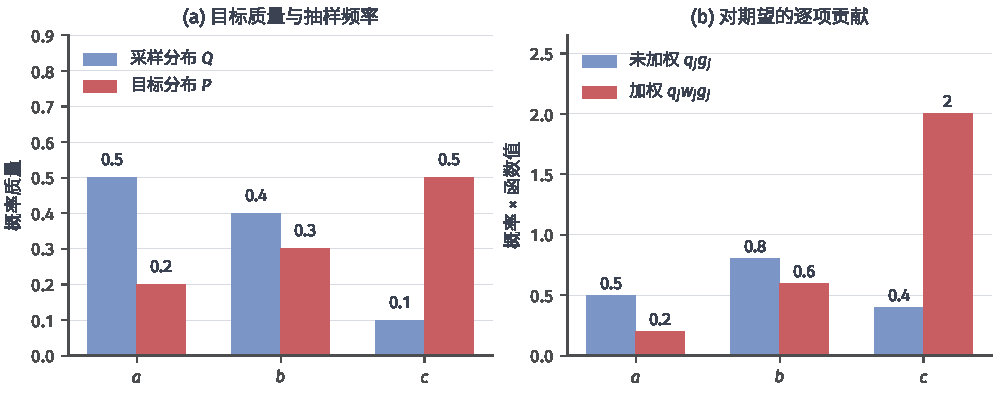
\includegraphics[width=\linewidth]{figures/01-mathematical-preliminaries/04-random-variables-distributions-and-causality/matplotlib/probability-importance-weights/figure.pdf}
  \caption{三结果换测度的有限构造。左图比较采样分布\(Q\)与目标分布\(P\)，右图比较\(q_jg_j\)与\(q_jw_jg_j=p_jg_j\)。各柱从零起画；右图柱高之和分别为\(1.7\)和\(2.8\)，并非单点概率。}
  \label{fig:probability-importance-weights}
\end{figure*}

绝对连续性也决定几乎处处结论能否转移。若\(P\ll Q\)，且
\(|g|\leq M\)在\(Q\)下几乎处处成立，则违背上界的集合是\(Q\)-零集，因而也是
\(P\)-零集；同一上界在\(P\)下仍成立。反向转移需要\(Q\ll P\)，不能只凭
\(P\ll Q\)得到。若\(|g|\leq B\)，则
\[
  \mathbb{E}_Q[w^2g^2]\leq B^2\mathbb{E}_Q[w^2],
\]
所以权重二阶矩有限是有界被积函数获得有限重加权方差的充分条件。把权重截为
\(w_c=\min\{w,c\}\)会限制波动，但
\(\mathbb{E}_Q[w_cg]\)与\(\mathbb{E}_P[g]\)之差为
\(-\mathbb{E}_Q[(w-c)_+g]\)，一般不为零。

% Baseline P:628-716
设\(Q\ll P\)，并记\(L=\mathrm{d}Q/\mathrm{d}P\)。对\(X\in L^1(Q)\)，在\(\mathbb{E}_P[L\mid\mathcal{G}]>0\)处有
\begin{equation}
  \mathbb{E}_Q[X\mid\mathcal{G}]
  =
  \frac{\mathbb{E}_P[LX\mid\mathcal{G}]}
       {\mathbb{E}_P[L\mid\mathcal{G}]}.
  \label{eq:probability-conditional-change-measure}
\end{equation}
为验证这个候选变量确实是条件期望，记
\[
  D=\mathbb{E}_P[L\mid\mathcal{G}],
  \qquad
  N=\mathbb{E}_P[LX\mid\mathcal{G}],
\]
并在\(\{D>0\}\)上令\(Z=N/D\)，在\(\{D=0\}\)上令\(Z=0\)。分母零集在\(Q\)下可以忽略，因为
\[
  Q(D=0)
  =
  \mathbb{E}_P[L\mathbb{I}\{D=0\}]
  =
  \mathbb{E}_P[D\mathbb{I}\{D=0\}]
  =0.
\]
条件期望的单调性还给出
\[
  |N|
  \leq
  \mathbb{E}_P[L|X|\mid\mathcal{G}].
\]
在\(\{D=0\}\)上，非负变量\(L\mathbb{I}\{D=0\}\)的期望为零，因而\(L=0\)几乎处处。于是
\[
  \mathbb{E}_P\left[
    \mathbb{E}_P[L|X|\mid\mathcal{G}]
    \mathbb{I}\{D=0\}
  \right]
  =
  \mathbb{E}_P[L|X|\mathbb{I}\{D=0\}]
  =0,
\]
上面的条件三角不等式进而说明\(N=0\)在\(\{D=0\}\)上几乎处处成立。因此\(DZ=N\)几乎处处，而且
\[
  \begin{aligned}
    \mathbb{E}_Q|Z|
    &=
    \mathbb{E}_P[L|Z|]
    =
    \mathbb{E}_P[D|Z|]\\
    &=
    \mathbb{E}_P\bigl[|N|\mathbb{I}\{D>0\}\bigr]
    \leq
    \mathbb{E}_P[L|X|]
    =
    \mathbb{E}_Q|X|<\infty.
  \end{aligned}
\]
这里把\(\mathcal{G}\)-可测的非负因子\(|Z|\)提出条件期望，可以由有界截断和单调收敛得到。候选变量的可积性建立后，对
\(A\in\mathcal{G}\)可合法地计算
\[
  \begin{aligned}
    \int_A Z\,\mathrm{d}Q
    &=
    \int_A ZL\,\mathrm{d}P
    =
    \int_A Z\mathbb{E}_P[L\mid\mathcal{G}]\,\mathrm{d}P\\
    &=
    \int_A \mathbb{E}_P[LX\mid\mathcal{G}]\,\mathrm{d}P
    =
    \int_A LX\,\mathrm{d}P
    =
    \int_A X\,\mathrm{d}Q.
  \end{aligned}
\]
因此\(Z\)满足\(X\)在\(Q\)下关于\(\mathcal{G}\)的条件期望定义。公式\eqref{eq:probability-conditional-change-measure}是Bayes更新的一般测度形式；
分母零集与候选变量可积性都需要像上面这样核对。

用有限分组可以看出分母为何不可省略。设参考分布\(P\)把四个结果
\(\omega_1,\ldots,\omega_4\)分别赋予概率\((0.4,0.1,0.1,0.4)\)，目标分布
\(Q\)赋予\((0.1,0.5,0.1,0.3)\)。令信息\(\mathcal{G}\)只区分
\(A=\{\omega_1,\omega_2\}\)和\(A^{\mathsf c}\)，并令
\(X=(0,1,0,1)\)。权重\(L\)在四点上的值为\((0.25,5,1,0.75)\)。在\(A\)内，
\[
  \mathbb{E}_P[LX\mid\mathcal{G}]
  =\frac{0.5}{0.5}=1,\qquad
  \mathbb{E}_P[L\mid\mathcal{G}]
  =\frac{0.1+0.5}{0.5}=1.2,
\]
所以目标条件均值为\(1/1.2=5/6\)，与
\(\mathbb{E}_Q[X\mid A]=0.5/(0.1+0.5)\)一致。
省略分母却会得到\(1\)，可以直接看到重新归一化改变了答案。
在\(A^{\mathsf c}\)内，分子为\(0.3/0.5=0.6\)，分母为\(0.4/0.5=0.8\)，
相除得到\(3/4\)，也等于该组在\(Q\)下的条件均值。
条件化后必须按每个信息分组的目标总质量分别归一化。
对有限联合观测\(X_1,\ldots,X_n\)，若在同一逐步参考核下，两个规律的条件密度分别为
\(p_i(x_i\mid x_{<i})\)、\(q_i(x_i\mid x_{<i})\)，且初始及逐步目标核对来源核绝对连续，则
\[
\frac{\mathrm dQ}{\mathrm dP}(x_{1:n})
=\prod_{i=1}^n
\frac{q_i(x_i\mid x_{<i})}{p_i(x_i\mid x_{<i})}
\quad P\text{-几乎处处}.
\]
每个比值都要条件可测，并在实际可能到达的历史上归一化；对\(P\)不可能产生而\(Q\)可能产生的观测，不能用有限权重补救。此式只依赖联合分布的链式分解，不预设Markov性。核因子何时可以相消，在第~\ref{sec:rv-markov}节另行核对。

\section{随机序列和随机过程}
\label{sec:rv-sequences-processes}
\label{sec:probability-averages-errors}
重复观测使问题从单个变量变成变量族。固定样本量时，要控制和、平均或整组候选的误差；样本量增长时，要规定极限的含义。把索引进一步解释为时间，还需描述历史信息与整条路径，不能只盯着每一时刻的边缘分布。

\subsection{随机序列}
\label{sec:rv-sequences}
\begin{definition}[随机序列]
\label{def:rv-random-sequence}
同一概率空间上的可测映射族\((X_n)_{n\in\mathbb N}\)称为\term{随机序列}（random sequence）。固定\(n\)得到一个随机变量，固定\(\omega\)得到确定的实现序列
\((X_n(\omega))_{n\in\mathbb N}\)。取值空间可以是实数、向量或其他指定可测空间。
\end{definition}
例如独立噪声\((\varepsilon_i)\)、共享背景的读数
\(X_i=\Theta+\varepsilon_i\)和累计和
\(S_n=\sum_{i=1}^n\varepsilon_i\)都是随机序列，但具有不同的联合关系。前者可独立，中者共享\(\Theta\)，后者相邻项共享此前的全部增量。即使各项边缘相同，也不能据此选用独立样本平均的结论。这里\(n\)可以是试验编号；当它表示物理时间或算法轮次时，历史信息的解释才进一步进入模型。

\subsection{随机序列的聚合}
\label{sec:rv-aggregation}
有限样本误差回答“现有\(n\)次观测是否足够”。下面先对一个累计量给出概率界，再对候选族同时控制，最后把这些工具用于积分计算。后续极限定理不会自动给出这些有限样本常数。

\subsubsection{累计量的概率误差}
\label{sec:probability-basic-tail-bounds}
\label{sec:probability-concentration-inequalities}
% Baseline P:1288-1308

从矩推出收敛关系之前，先建立两条最基本的尾界。若\(X\geq0\)，则对\(a>0\)，
\begin{equation}
  \mathbb{P}(X\geq a)
  \leq
  \frac{\mathbb{E}X}{a}.
  \label{eq:probability-markov-inequality}
\end{equation}
证明只需写
\(\mathbb{E}X\geq
\mathbb{E}[X\mathbb{I}\{X\geq a\}]
\geq a\mathbb{P}(X\geq a)\)。
这就是Markov不等式。对均值\(\mu\)、方差\(\sigma^2<\infty\)的随机变量，把
Markov不等式用于\((X-\mu)^2\)，得到Chebyshev不等式
\begin{equation}
  \mathbb{P}(|X-\mu|\geq t)
  \leq\frac{\sigma^2}{t^2},
  \qquad t>0.
  \label{eq:probability-chebyshev-inequality}
\end{equation}
它只使用二阶矩，因而适用范围广，但没有利用有界性或指数矩信息。
% Baseline P:1698-1841
对任意\(\lambda>0\)，函数\(x\mapsto e^{\lambda x}\)单调。Markov不等式给出
\begin{equation}
  \mathbb{P}(X\geq t)
  =
  \mathbb{P}(e^{\lambda X}\geq e^{\lambda t})
  \leq
  e^{-\lambda t}\mathbb{E}[e^{\lambda X}].
  \label{eq:probability-chernoff-step}
\end{equation}
随后对\(\lambda\)优化，便得到Chernoff方法。整个方法依赖相应指数矩有限；若\(\mathbb{E}e^{\lambda X}=\infty\)，式
\eqref{eq:probability-chernoff-step}虽形式上仍真，却不给出有用上界。

\begin{definition}[次高斯变量]
  \label{def:probability-subgaussian}
对\(\sigma^2>0\)，均值为零的可积实随机变量\(X\)若满足
\[ \mathbb{E}[e^{\lambda X}]
  \leq\exp\left(\frac{\lambda^2\sigma^2}{2}\right),\qquad \lambda\in\mathbb{R}, \]
就称它为参数\(\sigma^2\)的\term{次高斯变量}（sub-Gaussian random variable）。
\end{definition}
代入Chernoff界并取\(\lambda=t/\sigma^2\)，得到
\[ \mathbb{P}(X\geq t)
  \leq\exp\left(-\frac{t^2}{2\sigma^2}\right). \]
“次高斯”描述的是指数矩或尾部上界，不表示变量本身服从高斯分布。

\par\medskip\noindent\textbf{有界变量的Hoeffding不等式}\quad
\begin{lemma}[Hoeffding引理]
\label{lem:probability-hoeffding-lemma}
若\(\mathbb{E}X=0\)且\(X\in[a,b]\)几乎处处成立，则
\[ \mathbb{E}[e^{\lambda X}]
  \leq\exp\left\{\frac{\lambda^2(b-a)^2}{8}\right\},\qquad \lambda\in\mathbb{R}. \]
\end{lemma}

\begin{proof}
若\(a=b\)，均值为零迫使\(X=0\)，结论直接成立。以下设\(a<b\)。
凸性说明，对\(x\in[a,b]\)，指数函数位于连接端点的弦下方：
\[ e^{\lambda x}
  \leq\frac{b-x}{b-a}e^{\lambda a}+\frac{x-a}{b-a}e^{\lambda b}. \]
取期望并使用\(\mathbb{E}X=0\)。令\(p=-a/(b-a)\in[0,1]\)、
\(s=\lambda(b-a)\)，则右侧的对数为
\[
 \psi(s)=\log\bigl[(1-p)e^{-ps}+pe^{(1-p)s}\bigr].
\]
这里对无量纲变量\(s\)求导。写
\(r_s=pe^s/(1-p+pe^s)\)，直接求导得到
\(\psi''(s)=r_s(1-r_s)\leq1/4\)，且\(\psi(0)=\psi'(0)=0\)。
Taylor积分余项给出
\(\psi(s)=s^2\int_0^1(1-u)\psi''(us)\,\mathrm du\leq s^2/8\)，
对正负\(s\)都成立。代回原变量，便有
\[ \log\mathbb{E}[e^{\lambda X}]
  \leq\frac{\lambda^2(b-a)^2}{8}. \]
指数化即得结论。
\end{proof}

\begin{theorem}[Hoeffding不等式]
\label{thm:probability-hoeffding-inequality}
设\(X_1,\ldots,X_n\)相互独立，且\(X_i\in[a_i,b_i]\)几乎处处成立。则对\(t>0\)，
\[
  \mathbb{P}\left(
    \sum_{i=1}^{n}(X_i-\mathbb{E}X_i)\geq t
  \right)
  \leq
  \exp\left\{
    -\frac{2t^2}{\sum_{i=1}^{n}(b_i-a_i)^2}
  \right\}.
\]
\end{theorem}

\begin{proof}
记\(S=\sum_i(X_i-\mathbb{E}X_i)\)。对\(\lambda>0\)，独立性使指数矩分解：
\[
\begin{aligned}
  \mathbb{P}(S\geq t)
  &\leq
  e^{-\lambda t}\mathbb{E}[e^{\lambda S}]\\
  &=
  e^{-\lambda t}
  \prod_{i=1}^{n}
  \mathbb{E}\left[
    e^{\lambda(X_i-\mathbb{E}X_i)}
  \right]\\
  &\leq
  \exp\left\{
    -\lambda t+
    \frac{\lambda^2}{8}
    \sum_{i=1}^{n}(b_i-a_i)^2
  \right\}.
\end{aligned}
\]
右侧关于\(\lambda\)的最小点为
\[ \lambda^\star
  =\frac{4t}{\sum_i(b_i-a_i)^2}. \]
代回即得结论。对\(-S\)使用同一结果，再用联合界可得双侧版本。
\end{proof}

若\(X_i\in[0,1]\)独立，则样本平均满足
\[ \mathbb{P}(|\overline{X}_n-\mathbb{E}\overline{X}_n|
  \geq\varepsilon)\leq 2e^{-2n\varepsilon^2}. \]
有界性进入Hoeffding引理，独立性进入矩母函数乘积；删除任一条件都不能沿用这份证明。

\par\medskip\noindent\textbf{方差敏感的Bernstein不等式}\quad
若独立中心化变量满足\(|X_i|\leq M\)，并记\(v=\sum_i\mathbb{E}[X_i^2]\)，则Bernstein不等式的一个版本为
\begin{equation}
  \mathbb{P}\left(\sum_{i=1}^{n}X_i\geq t\right)
  \leq
  \exp\left\{
    -\frac{t^2}{2(v+Mt/3)}
  \right\}.
  \label{eq:probability-bernstein-inequality}
\end{equation}
为看清两个尺度的来源，取\(0<\lambda<3/M\)。由指数级数及
\(|X_i|^k\leq M^{k-2}X_i^2\)（\(k\geq2\)），有
\[
  \mathbb{E}e^{\lambda X_i}
  \leq
  1+\frac{\lambda^2\mathbb{E}X_i^2}
           {2(1-\lambda M/3)}
  \leq
  \exp\left\{
    \frac{\lambda^2\mathbb{E}X_i^2}
         {2(1-\lambda M/3)}
  \right\}.
\]
这里第一阶项因中心化而消失，常数\(1/3\)来自用几何级数控制
\[
  \sum_{k\geq3}\frac{(\lambda M)^{k-2}}{k!}.
\]
独立性使各指数矩相乘，Chernoff步骤于是给出
\[
  \mathbb{P}\left(\sum_iX_i\geq t\right)
  \leq
  \exp\left\{
    -\lambda t+\frac{\lambda^2v}
      {2(1-\lambda M/3)}
  \right\}.
\]
取\(\lambda=t/(v+Mt/3)\)便得到式~\eqref{eq:probability-bernstein-inequality}。小偏差区域由\(v\)主导，呈高斯型；大偏差区域由\(Mt\)主导，呈指数型。

例如\(B_i\sim\operatorname{Bernoulli}(0.01)\)独立，考虑
\(\overline{B}_n-0.01\geq0.05\)。Hoeffding上界为
\(\exp(-0.005n)\)，而Bernstein上界约为
\[
  \exp\left\{
    -\frac{0.05^2n}
      {2(0.01\times0.99+0.05/3)}
  \right\}
  \approx \exp(-0.047n).
\]
低发生率使实际方差远小于区间最坏尺度，所以后者明显更紧；当方差接近区间允许的最大值或偏差进入线性尺度时，Bernstein并不保证处处优于Hoeffding。

对重尾变量，方差可能不存在，指数矩也可能对所有正参数发散。此时Chebyshev、Hoeffding和Bernstein各自在矩、范围或指数矩步骤失效。可以增加截断、稳健均值或仅用
有限\(p\)阶矩推导多项式尾界，但所得估计对象和偏差需要重新说明，不能继续声称高斯型集中。

\subsubsection{候选族的共同误差}
\label{sec:probability-uniform-errors-symmetry}
\label{sec:probability-random-functions-uniform-error}
一个候选的误差小，不保证由同一数据选中的候选误差也小。若要允许选择，应先在同一概率事件上控制全部候选。候选索引与样本索引在这里并存，不能把“每个固定候选都成立”误读成“所有候选同时成立”。

\paragraph{有限候选的联合控制}
% Baseline P:1855-1917
设有限候选类\(\mathcal{H}=\{h_1,\ldots,h_M\}\)，损失\(\ell(h,Z)\in[0,1]\)。真实风险与经验风险分别为
\[ R(h)=\mathbb{E}[\ell(h,Z)],
  \qquad\widehat{R}_n(h)=\frac{1}{n}\sum_{i=1}^{n}\ell(h,Z_i), \]
其中\(Z_1,\ldots,Z_n\)独立同分布。对预先固定的单个\(h\)，Hoeffding不等式给出
\[ \mathbb{P}\bigl(
    |\widehat{R}_n(h)-R(h)|>\varepsilon\bigr)\leq 2e^{-2n\varepsilon^2}. \]
但经验最优候选
\(\widehat{h}\in\arg\min_h\widehat{R}_n(h)\)由同一批数据选出，不是预先固定对象。只控制一个候选不能排除“恰好因噪声看起来最好”的选择偏差。

为明确“同时控制”与“样本量足够”的关系，把上述要求写成一个定义。这里讨论抽样前固定的函数类；所有上确界均假定可测。一项常用充分条件是存在可数子类，使每个函数都是该子类中某个序列的逐点极限。
\begin{definition}[分布无关的一致收敛]
  \label{def:uniform-convergence}
  设\(\mathcal G\)是非空的\([0,1]\)值可测函数类。若对任意\(\eta,\delta\in(0,1)\)，存在只依赖\(\mathcal G,\eta,\delta\)的整数\(n_0\)，使任意概率分布\(P\)和任意\(n\geq n_0\)的独立同分布样本\(S=(Z_1,\ldots,Z_n)\sim P^n\)均满足
  \begin{equation}
    \mathbb P_{S\sim P^n}\left\{
      \sup_{g\in\mathcal G}\left|\frac1n\sum_{i=1}^ng(Z_i)-\mathbb E_Pg\right|\leq\eta
    \right\}\geq1-\delta,
    \label{eq:uniform-convergence-definition}
  \end{equation}
  就称\(\mathcal G\)满足分布无关的\term{一致收敛}（uniform convergence）。若只要求\(P\)属于指定分布族，同一定义给出相对于该分布族的一致收敛。
\end{definition}
“函数上一致”由上确界表达，“分布无关”则要求同一个\(n_0\)适用于全部允许分布。对每个固定函数或每个固定分布分别存在的样本量，不能自动满足这两个量词。

\begin{theorem}[有限函数类的一致误差界]
\label{thm:probability-finite-class-uniform-bound}
在上述条件下，对任意\(\delta\in(0,1)\)，以至少\(1-\delta\)的概率同时对所有\(h\in\mathcal{H}\)有
\begin{equation}
  |\widehat{R}_n(h)-R(h)|
  \leq
  \sqrt{\frac{\log(2M/\delta)}{2n}}.
  \label{eq:probability-finite-class-bound}
\end{equation}
\end{theorem}

\begin{proof}
对每个\(h\)定义坏事件
\[ A_h=
  \{|\widehat{R}_n(h)-R(h)|>\varepsilon\}. \]
单函数Hoeffding界给出\(\mathbb{P}(A_h)\leq2e^{-2n\varepsilon^2}\)。由联合界，
\[ \mathbb{P}\left(\bigcup_{h\in\mathcal{H}}A_h\right)
  \leq 2M e^{-2n\varepsilon^2}. \]
令右侧等于\(\delta\)，解得\(\varepsilon=\sqrt{\log(2M/\delta)/(2n)}\)。在坏事件并集的补集上，结论对
全部候选同时成立。
\end{proof}

令\(h^\star\in\arg\min_hR(h)\)，并在式\eqref{eq:probability-finite-class-bound}成立的事件上记右侧为\(\varepsilon_n\)。则
\[
\begin{aligned}
  R(\widehat{h})
  &\leq
  \widehat{R}_n(\widehat{h})+\varepsilon_n\\
  &\leq
  \widehat{R}_n(h^\star)+\varepsilon_n\\
  &\leq
  R(h^\star)+2\varepsilon_n.
\end{aligned}
\]
第二步正是经验最优性的用途。候选数只通过\(\log M\)进入，但若候选类本身由同一数据任意生成，简单地把最终数量代入\(M\)未必合法；需要把生成过程纳入统一控制对象。
例如\(M=100\)、\(n=1000\)、\(\delta=0.05\)时，式~\eqref{eq:probability-finite-class-bound}右侧约为
\[
  \sqrt{\frac{\log 4000}{2000}}\approx0.0644.
\]
这个数同时控制一百个预先固定候选，而不是给每个候选各自提供\(95\%\)保证；后一做法的联合失败概率可能远大于\(5\%\)。
% Baseline P:1974-2031

\begin{lemma}[\(\chi^2\)变量的尾界]
  \label{lem:probability-chi-square-tail}
  若\(Z\sim\chi_k^2\)，其中\(k\)为正整数，则对每个\(x>0\)，
  \[
    \mathbb{P}\{Z-k\geq2\sqrt{kx}+2x\}\leq e^{-x},
    \qquad
    \mathbb{P}\{k-Z\geq2\sqrt{kx}\}\leq e^{-x}.
  \]
  因而对\(0<\varepsilon<1\)，
  \begin{equation}
    \mathbb{P}\left(
      \left|\frac{Z}{k}-1\right|>\varepsilon
    \right)
    \leq2\exp\left(-\frac{k\varepsilon^2}{8}\right).
    \label{eq:probability-chi-square-relative-tail}
  \end{equation}
\end{lemma}

\begin{proof}
标准高斯积分给出\(\mathbb E e^{\lambda G^2}=(1-2\lambda)^{-1/2}\)，\(\lambda<1/2\)。独立性因而给出
\[
  \log\mathbb E e^{\lambda(Z-k)}
  =\frac{k}{2}\{-2\lambda-\log(1-2\lambda)\}
  \leq\frac{k\lambda^2}{1-2\lambda},\qquad 0<\lambda<1/2.
\]
最后一步来自\(-u-\log(1-u)=\sum_{j\geq2}u^j/j\leq u^2/[2(1-u)]\)。对上尾使用Chernoff方法，取
\(\lambda=\sqrt{x}/(\sqrt{k}+2\sqrt{x})\)，便在阈值\(2\sqrt{kx}+2x\)处得到指数\(-x\)。
对下尾，用\(u-\log(1+u)\leq u^2/2\)得到
\[
  \log\mathbb E e^{-\lambda(Z-k)}\leq k\lambda^2,\qquad\lambda>0.
\]
取\(\lambda=\sqrt{x/k}\)，在阈值\(2\sqrt{kx}\)处也得到指数\(-x\)。最后取\(x=k\varepsilon^2/8\)。当\(0<\varepsilon<1\)时，两侧阈值均不超过\(k\varepsilon\)，故相对偏差事件包含于对应尾事件的并集，联合界给出式~\eqref{eq:probability-chi-square-relative-tail}。
\end{proof}

现在把单个方向的集中推广到有限点集。这一结果称为Johnson--Lindenstrauss引理：保留有限个距离所需的随机投影维数主要随点数的对数增长，而不由原始坐标数直接决定。
\begin{theorem}[高斯随机投影的距离保持]
  \label{thm:probability-johnson-lindenstrauss}
  给定抽样前固定的\(N\geq2\)个点\(\bm x_1,\ldots,\bm x_N\in\mathbb R^d\)，以及\(\varepsilon,\delta\in(0,1)\)。若\(\bm A\in\mathbb R^{k\times d}\)的元素独立服从\(\mathcal N(0,1/k)\)，且
  \[
    k\geq\frac8{\varepsilon^2}\log\frac{N(N-1)}\delta,
  \]
  则以至少\(1-\delta\)的概率，对全部\(i,j\)同时有
  \begin{equation}
    (1-\varepsilon)\|\bm x_i-\bm x_j\|_2^2
    \leq\|\bm A\bm x_i-\bm A\bm x_j\|_2^2
    \leq(1+\varepsilon)\|\bm x_i-\bm x_j\|_2^2.
    \label{eq:probability-jl-distance-preservation}
  \end{equation}
\end{theorem}
\begin{proof}
固定一个不依赖\(\bm A\)的非零向量\(\bm v\)。矩阵各行独立，每个\((\bm A\bm v)_r\)均为均值零、方差\(\|\bm v\|_2^2/k\)的高斯变量，因此
\[
  \frac{k\|\bm A\bm v\|_2^2}{\|\bm v\|_2^2}\sim\chi_k^2.
\]
引理~\ref{lem:probability-chi-square-tail}使该方向的相对平方范数失真概率不超过\(2e^{-k\varepsilon^2/8}\)。点对差至多有\(N(N-1)/2\)个；对全部非零差使用联合界，失败概率不超过\(N(N-1)e^{-k\varepsilon^2/8}\leq\delta\)。零差经任何线性投影仍为零，无须额外尾界。
\end{proof}
结论控制的是平方距离；对距离本身开方后，因子为\(\sqrt{1\pm\varepsilon}\)。点集须在投影抽样前确定，但在同时保持事件上，可以事后任选这批点中的一对查询。它不保证对观察到\(\bm A\)后任意新造的向量都保持范数；当\(k<d\)时，\(\bm A\)的非零零空间方向就给出反例。这里的常数是便于推导的充分界，也不保证所得\(k\)一定小于\(d\)。

\paragraph{无限候选的统一控制}
% Baseline P:1921-1961
无限函数类不能直接按元素做联合界。第~\ref{sec:comb-families-counting}节建立的取值模式与
第~\ref{sec:functional-combinatorial-metric-complexity}节建立的覆盖数提供两种
有限化方法。使用样本取值模式时，须先引入独立样本副本并进行下文的对称化，再条件于两批合并样本。此时随机符号和只由样本上的有限取值模式决定，才可对模式使用条件尾界和联合界。同一个样本模式可能对应不同的真实风险，因此不能直接把前面固定候选界中的\(M\)换成当前样本的模式数。
使用覆盖网时，若每个函数都能由有限\(\varepsilon\)-网中的代表逼近，则先控制网点，再用Lipschitz性质把误差转回原函数。下面先建立后一种方法所需的误差比较，再说明对称化怎样引入随机符号。

\begin{lemma}[覆盖数的有限网控制]
  \label{lem:probability-covering-finite-net}
  设\((\mathcal{F},d)\)具有有限\(\varepsilon\)-网
  \(\mathcal{N}_\varepsilon\)，其大小为
  \(N(\mathcal{F},d,\varepsilon)\)。若随机过程
  \(\{Z_f:f\in\mathcal{F}\}\)满足
  \[
    |Z_f-Z_g|\leq Ld(f,g)
  \]
  几乎处处对所有\(f,g\)成立，并且相关上确界可测，则对任意\(t>0\)，
  \begin{equation}
    \mathbb{P}\left\{
      \sup_{f\in\mathcal{F}}|Z_f|>t+L\varepsilon
    \right\}
    \leq
    N(\mathcal{F},d,\varepsilon)
    \sup_{f\in\mathcal{F}}\mathbb{P}(|Z_f|>t).
    \label{eq:probability-covering-finite-net}
  \end{equation}
\end{lemma}

\begin{proof}
对每个\(f\)选取满足\(d(f,g_f)\leq\varepsilon\)的
\(g_f\in\mathcal{N}_\varepsilon\)。则
\[
  |Z_f|\leq |Z_{g_f}|+L\varepsilon,
\]
所以左侧坏事件包含在
\(\bigcup_{g\in\mathcal{N}_\varepsilon}\{|Z_g|>t\}\)中。对这个有限并集使用联合界
即得结论。
\end{proof}

若\(Z_f=\widehat R_n(f)-R(f)\)，且经验风险与真实风险各自关于\(d\)都是
\(L_0\)-Lipschitz，则引理中的过程常数是\(2L_0\)。因此，网格大小、离散误差
\(2L_0\varepsilon\)和单点尾界必须一起进入结论；只报告覆盖数而不验证Lipschitz传递
还不能控制原函数类。

% Baseline P:2035-2049
有些目标不是单个样本平均，而是整个数据集的函数\(F(Z_1,\ldots,Z_n)\)。若替换第\(i\)个输入最多改变\(c_i\)，即
\[ \sup_{\bm{z},z_i'}
  |F(z_1,\ldots,z_i,\ldots,z_n)-F(z_1,\ldots,z_i',\ldots,z_n)|\leq c_i, \]
则独立输入下的McDiarmid不等式给出
\begin{equation}
  \mathbb{P}\bigl(
    F-\mathbb{E}F\geq t
  \bigr)
  \leq
  \exp\left\{
    -\frac{2t^2}{\sum_{i=1}^{n}c_i^2}
  \right\}.
  \label{eq:probability-mcdiarmid}
\end{equation}
其证明把\(F\)依次对前\(i\)个观测条件化，形成Doob鞅；每步有界差控制一个鞅增量，再使用Hoeffding型指数矩界。独立性保证逐步揭示观测时的条件结构，有界差则限制单个观测的影响。
McDiarmid不等式的完整证明见第~\ref{sec:rv-fixed-time}节：在那里把数据函数逐步揭示为Doob鞅，并说明独立输入为什么给出所需的条件范围。
% Baseline P:2053-2272
有限候选可按数量控制误差；无限类的函数在同一组观测上可能高度相似，直接计数会忽略这种结构。\term{Rademacher复杂度}提供另一种衡量方式：固定观测点后，让函数尽量对齐一组无信号的随机正负号，再对这些正负号平均。能拟合更多随机起伏的类，需要更大的同时误差代价。
\begin{definition}[经验Rademacher复杂度]
  \label{def:rademacher-complexity}
  给定非空实值可测函数类\(\mathcal G\)和样本\(S=(z_1,\ldots,z_n)\)。令\(\sigma_i\)独立且等概率取\(-1,1\)。当上确界可测且期望有限时，\term{经验Rademacher复杂度}定义为
  \begin{equation}
    \widehat{\mathfrak R}_S(\mathcal G)
    =\mathbb E_\sigma\left[\sup_{g\in\mathcal G}\frac1n\sum_{i=1}^n\sigma_i g(z_i)\right].
    \label{eq:empirical-rademacher}
  \end{equation}
\end{definition}
固定的是样本，不是使随机和最大的函数；每一组符号都允许选择不同函数。交换上确界与期望会把所有固定函数的零均值随机和平均成零，丢掉所要衡量的拟合能力。
\begin{definition}[期望Rademacher复杂度]
  \label{def:expected-rademacher-complexity}
  对\(S\sim P^n\)，\term{期望Rademacher复杂度}定义为
  \[
    \mathfrak R_n(\mathcal G)=\mathbb E_{S\sim P^n}\widehat{\mathfrak R}_S(\mathcal G).
  \]
\end{definition}
期望复杂度还平均了抽样结果，故依赖\(P\)；经验复杂度仅依赖给定样本上的函数取值。
允许函数作凸组合会增加候选函数，却未必增加它们对随机符号的最大对齐能力。
原因在于，固定符号后，经验随机和是函数取值的线性泛函：若一个组合的各项都不超过
同一个上界，非负且归一化的加权平均也不能超过它。下面把这一几何性质写成复杂度恒等式。

\begin{theorem}[凸组合的Rademacher复杂度]
\label{thm:ensemble-convex-hull}
设$S=(z_1,\ldots,z_n)$为固定样本，$n\geq1$，$\mathcal B$为非空实值可测函数类，
且在这组样本上统一有界，即存在有限$M$使$|h(z_i)|\leq M$对所有
$h\in\mathcal B$和$i$成立。令
\[
 \operatorname{conv}(\mathcal B)
 =\left\{\sum_{t=1}^T a_t h_t:
 T\geq1,\ h_t\in\mathcal B,\ a_t\geq0,\ \sum_{t=1}^T a_t=1\right\}
\]
为全部有限凸组合构成的函数类。则
\[
 \widehat{\mathfrak R}_S(\operatorname{conv}(\mathcal B))
 =\widehat{\mathfrak R}_S(\mathcal B).
\]
若样本再按$P^n$抽取，几乎必然满足上述样本有界条件，且相应样本上确界可测、期望有限，
则期望Rademacher复杂度也满足同一恒等式。
\end{theorem}

\begin{proof}
固定一组符号$\bm\sigma$。对任意有限凸组合，由$a_t\geq0$和$\sum_ta_t=1$，
\[
 \begin{aligned}
 \frac1n\sum_{i=1}^n\sigma_i\sum_{t=1}^T a_t h_t(z_i)
 &=\sum_{t=1}^T a_t
    \left(\frac1n\sum_{i=1}^n\sigma_i h_t(z_i)\right)\\
 &\leq\sup_{h\in\mathcal B}\frac1n\sum_{i=1}^n\sigma_i h(z_i).
 \end{aligned}
\]
因此凸包上的上确界不超过基类上的上确界。反向不等式来自
$\mathcal B\subseteq\operatorname{conv}(\mathcal B)$：取$T=1$即可得到任意基函数。
于是每一组符号下的两个上确界都相等。样本上的统一有界性保证随机和与其上确界有限，
对$\bm\sigma$取期望便得经验复杂度恒等式；在额外的抽样可测性与可积条件下，再对$S$
取期望即得期望复杂度结论。证明不要求函数类有限，也不要求上确界由某个函数达到。
\end{proof}

例如，只含常值函数$0$和$1$的基类，其凸包包含全部常值$c\in[0,1]$。
固定一个观测点时，正号下的最大随机和为$1$，负号下为$0$，两类的经验复杂度都为
$1/2$。候选函数从两个增加到无穷多个，但线性随机和的最坏值仍由端点决定。
这一定理只控制实值函数的随机线性和；把组合再作阈值化等非线性变换后，
需要另外分析变换后的函数类。非负性与归一化也是凸组合的条件，不能用同一等式处理
任意符号或任意尺度的线性组合。

\begin{definition}[经验高斯复杂度]
  \label{def:gaussian-complexity}
  将随机符号换成独立标准高斯系数\(\xi_i\sim\mathcal N(0,1)\)，定义
  \[
    \widehat{\mathfrak G}_S(\mathcal G)
    =\mathbb E_\xi\left[\sup_{g\in\mathcal G}\frac1n\sum_{i=1}^n\xi_i g(z_i)\right].
  \]
  相应期望高斯复杂度为\(\mathfrak G_n(\mathcal G)=\mathbb E_S\widehat{\mathfrak G}_S(\mathcal G)\)。
\end{definition}
高斯系数的符号与幅度都变化，Rademacher系数只有符号变化。二者是关于函数类的随机平均，不能按某一组系数的最大值直接比较。

双侧误差的证明常使用带绝对值版本
\[
  \widehat{\mathfrak R}^{\mathrm{abs}}_S(\mathcal G)
  =\mathbb E_\sigma\sup_{g\in\mathcal G}\left|\frac1n\sum_i\sigma_i g(z_i)\right|
  =\widehat{\mathfrak R}_S(\mathcal G\cup(-\mathcal G)),
\]
高斯版本同样定义。只有当\(\mathcal G=-\mathcal G\)时，两种约定才可直接等同。例如只含常数函数\(g\equiv1\)的类，其不带绝对值复杂度为\(0\)；带绝对值复杂度为\(n^{-1}\mathbb E|\sum_i\sigma_i|>0\)。以下对称化沿用带绝对值约定，后续应用单侧风险界时应核对所用版本。

\par\medskip\noindent\textbf{对称化与随机函数复杂度}\quad
设\(\mathcal{F}\)是一族取值于\([-1,1]\)的函数，定义
\[ \Delta(\bm{Z})
  =\sup_{f\in\mathcal{F}}\left|\mathbb{E}f(Z)-\frac{1}{n}\sum_{i=1}^{n}f(Z_i)\right|. \]
引入独立同分布副本\(Z_1',\ldots,Z_n'\)。Jensen不等式给出
\[
\begin{aligned}
  \mathbb{E}_{\bm{Z}}\Delta(\bm{Z})
  &\leq
  \mathbb{E}_{\bm{Z},\bm{Z}'}
  \sup_{f\in\mathcal{F}}
  \left|
    \frac{1}{n}\sum_{i=1}^{n}
    \bigl(f(Z_i')-f(Z_i)\bigr)
  \right|.
\end{aligned}
\]
由于每对\((Z_i,Z_i')\)交换后联合分布不变，引入独立Rademacher符号\(\sigma_i\in\{-1,1\}\)不会改变差的联合分布。因此
\[
  \mathbb{E}\Delta(\bm{Z})
  \leq
  2\mathbb{E}_{\bm{Z},\bm{\sigma}}
  \sup_{f\in\mathcal{F}}
  \left|
    \frac{1}{n}\sum_{i=1}^{n}\sigma_i f(Z_i)
  \right|.
\]
右侧是带绝对值的经验Rademacher复杂度对样本取期望后的两倍。它只在观测点上考察函数类与随机符号对齐的能力，把未知总体期望转成了条件于样本的随机和。

若\(\phi_i:\mathbb{R}\to\mathbb{R}\)均为\(L\)-Lipschitz且\(\phi_i(0)=0\)，则对任意不必关于取负封闭的函数类\(\mathcal{F}\)，带绝对值的收缩不等式为
\[
  \mathbb{E}_{\bm{\sigma}}
  \sup_{f\in\mathcal{F}}
  \left|
    \sum_i\sigma_i\phi_i(f(Z_i))
  \right|
  \leq
  2L\,
  \mathbb{E}_{\bm{\sigma}}
  \sup_{f\in\mathcal{F}}
  \left|
    \sum_i\sigma_i f(Z_i)
  \right|.
\]
一般情形需要先在取值向量类中临时加入零向量，再分别控制随机和的两个方向；这一步产生因子\(2\)。若变换后的取值向量类关于取负封闭，例如
\(\mathcal{F}=-\mathcal{F}\)且每个\(\phi_i\)都是奇函数，则可去掉该因子。这个不等式允许把预测函数的复杂度传到Lipschitz损失。若损失不全局Lipschitz或相关上确界不可积，必须限制作用范围或使用其他矩条件。

标量收缩可用逐坐标替换证明。先设函数类在固定样本上的取值向量组成有限集
\(\mathcal{A}\subset\mathbb{R}^n\)，并只考虑不带绝对值的上确界。固定前
\(n-1\)个符号，把相应部分记为\(U_{\bm{a}}\)。条件于这些符号，左侧最后一个坐标的贡献为
\[
  \frac12\sup_{\bm{a}}\{U_{\bm{a}}+\phi_n(a_n)\}
  +\frac12\sup_{\bm{a}}\{U_{\bm{a}}-\phi_n(a_n)\}.
\]
取两个上确界的近似最大元\(\bm{a},\bm{b}\)，并使用
\(\phi_n(a_n)-\phi_n(b_n)\leq L|a_n-b_n|\)。按
\(a_n-b_n\)的符号选择正负方向，便得到上式不超过
\[
  \frac12\sup_{\bm{a}}\{U_{\bm{a}}+La_n\}
  +\frac12\sup_{\bm{a}}\{U_{\bm{a}}-La_n\}.
\]
从最后一个坐标向前迭代，即得到单侧收缩。对随机和的正、负两个方向分别应用该结论，再用
\(\sup|S|=\max\{\sup S,\sup(-S)\}\)时，还需要保证两个单侧上确界非负。具体地，令
\(\mathcal{A}_0=\mathcal{A}\cup\{\bm{0}\}\)。由于\(\phi_i(0)=0\)，对每组固定符号都有
\[
\begin{aligned}
  \sup_{\bm{a}\in\mathcal{A}}
  \left|\sum_i\sigma_i\phi_i(a_i)\right|
  &\leq
  \sup_{\bm{a}\in\mathcal{A}_0}
  \sum_i\sigma_i\phi_i(a_i)
  +
  \sup_{\bm{a}\in\mathcal{A}_0}
  \left(-\sum_i\sigma_i\phi_i(a_i)\right).
\end{aligned}
\]
两个单侧上确界因包含零向量而非负。分别对\(\bm{\sigma}\)与\(-\bm{\sigma}\)应用单侧收缩，再利用二者同分布，得到
\[
  \mathbb{E}_{\bm{\sigma}}
  \sup_{\bm{a}\in\mathcal{A}}
  \left|\sum_i\sigma_i\phi_i(a_i)\right|
  \leq
  2L\,
  \mathbb{E}_{\bm{\sigma}}
  \sup_{\bm{a}\in\mathcal{A}_0}
  \sum_i\sigma_i a_i
  \leq
  2L\,
  \mathbb{E}_{\bm{\sigma}}
  \sup_{\bm{a}\in\mathcal{A}}
  \left|\sum_i\sigma_i a_i\right|.
\]
这就闭合了带绝对值版本的证明。一般函数类可由有限子类逼近并使用单调极限；不可数类还须保留前述可测性条件。

线性函数类展示了这一复杂度怎样落到熟悉的范数上。设
\[
  \mathcal{F}
  =\{\,\bm{z}\mapsto\langle\bm{w},\bm{z}\rangle:
       \lVert\bm{w}\rVert_2\leq B\,\},
  \qquad \lVert\bm{Z}_i\rVert_2\leq R.
\]
由对偶范数和Jensen不等式，
\[
\begin{aligned}
  \widehat{\mathfrak{R}}_{\bm{Z}}^{\mathrm{abs}}(\mathcal{F})
  &=
  \frac{B}{n}\mathbb{E}_{\bm{\sigma}}
  \left\lVert\sum_{i=1}^{n}\sigma_i\bm{Z}_i\right\rVert_2\\
  &\leq
  \frac{B}{n}
  \left(\sum_{i=1}^{n}\lVert\bm{Z}_i\rVert_2^2\right)^{1/2}
  \leq\frac{BR}{\sqrt n}.
\end{aligned}
\]
参数范数、样本范数和样本量分别进入\(B\)、\(R\)与\(n^{-1/2}\)。机器学习理论部分会在具体损失和模型类上继续把这一期望复杂度转换为高概率泛化界。

把Rademacher符号替换为独立标准高斯变量\(g_i\)，得到高斯复杂度
\[ \mathbb{E}_{\bm{g}}
  \sup_{f\in\mathcal{F}}
  \left|\frac{1}{n}\sum_i g_i f(Z_i)\right|. \]
记上述带绝对值的经验Rademacher复杂度和高斯复杂度分别为
\(\widehat{\mathfrak{R}}_{\bm{Z}}^{\mathrm{abs}}(\mathcal{F})\)与
\(\widehat{\mathfrak{G}}_{\bm{Z}}^{\mathrm{abs}}(\mathcal{F})\)。对任意固定样本，只要这些上确界可测且期望有限，就有单向比较
\[
  \widehat{\mathfrak{R}}_{\bm{Z}}^{\mathrm{abs}}(\mathcal{F})
  \leq
  \sqrt{\frac{\pi}{2}}\,
  \widehat{\mathfrak{G}}_{\bm{Z}}^{\mathrm{abs}}(\mathcal{F}).
\]
这个方向可直接由条件Jensen不等式解释：写\(g_i=\sigma_i|g_i|\)，符号与幅度独立，且\(\mathbb E|g_i|=\sqrt{2/\pi}\)。固定符号后，随机和的绝对值上确界是幅度向量的凸函数，先对幅度平均不大于先取上确界再平均，因而\(\widehat{\mathfrak G}^{\mathrm{abs}}_S\geq\sqrt{2/\pi}\,\widehat{\mathfrak R}^{\mathrm{abs}}_S\)。

反方向一般不能只付出普适常数。设函数类在固定样本上的取值向量恰为
\(\{\bm e_i,-\bm e_i:1\leq i\leq n\}\)，其中\(\bm e_i\)为第\(i\)个坐标向量。两个上确界分别化为
\[
 \widehat{\mathfrak R}^{\mathrm{abs}}_{\bm Z}=\frac1n,\qquad
 \widehat{\mathfrak G}^{\mathrm{abs}}_{\bm Z}
   =\frac{\mathbb E\max_{i\leq n}|g_i|}{n}.
\]
符号的绝对值恒为\(1\)，高斯幅度的最大值却随\(n\)增长。其尺度可直接核对：
对任意\(t>0\)，指数和上界及Jensen不等式给出
\[
 \mathbb E\max_i|g_i|
 \leq\frac{\log(2n)}t+\frac t2
 \leq\sqrt{2\log(2n)}
 \quad\text{当 }t=\sqrt{2\log(2n)}.
\]
下界取\(u=\sqrt{\log n}\geq1\)。在高斯密度积分中只保留区间
\([u,u+1/u]\)，得到
\(\mathbb P(|g_1|\geq u)\geq c\,u^{-1}e^{-u^2/2}\)，其中\(c>0\)为固定常数。
于是独立性给出
\[
 \mathbb P(\max_i|g_i|\geq u)
 \geq1-\exp\{-cn^{1/2}/\sqrt{\log n}\}\longrightarrow1.
\]
用期望下界\(u\,\mathbb P(\max_i|g_i|\geq u)\)可知，两种复杂度的比为
\(\Theta(\sqrt{\log n})\)（\(n\geq2\)，有限个小\(n\)并入常数）。
因此替换复杂度时必须保留比较方向；这个例子已经排除了普适常数的反向界。

\subsubsection{采样平均的积分近似}
\label{sec:probability-monte-carlo-variance-reduction}
% Baseline P:1518-1691
目标积分可统一写成
\[ I=\mathbb{E}_P[f(X)]. \]
若能独立采样\(X_i\sim P\)，直接蒙特卡洛估计为
\[ \widehat{I}_n
  =\frac{1}{n}\sum_{i=1}^{n}f(X_i). \]
当\(\mathbb E_P|f(X)|<\infty\)时，线性性给出无偏性；若方差
\(\sigma_f^2<\infty\)，则
\[ \operatorname{Var}(\widehat I_n)=\frac{\sigma_f^2}{n}. \]
长期一致性和缩放误差分布在第~\ref{sec:rv-aggregate-limits}节统一核验。
误差的标准差按\(n^{-1/2}\)下降，与输入维数没有显式关系，但
\(\sigma_f^2\)可能随问题结构急剧增大。

以下固定教学积分
\[ I=\int_0^1x^2\,\mathrm{d}x=\frac13. \]
若\(X\sim\operatorname{Unif}(0,1)\)，直接平均\(X_i^2\)的单样本方差为
\[ \operatorname{Var}(X^2)
  =\frac15-\frac19=\frac{4}{45}. \]

\par\medskip\noindent\textbf{重要性采样与方差}\quad
若\(P\ll Q\)，权重\(w=\mathrm{d}P/\mathrm{d}Q\)，则
\[ I=\mathbb{E}_Q[w(X)f(X)]. \]
从\(Q\)采样得到无偏估计
\begin{equation}
  \widehat{I}^{\mathrm{IS}}_n
  =
  \frac{1}{n}\sum_{i=1}^{n}w(X_i)f(X_i),
  \qquad X_1,\ldots,X_n\text{独立同分布于 }Q.
  \label{eq:probability-importance-sampling}
\end{equation}
无偏性只要求乘积可积；有限方差还要求\(\mathbb{E}_Q[w^2f^2]<\infty\)。

对上述积分，取\(Q\)的密度\(q(x)=2x\)，而\(P\)为均匀分布。除零测点\(x=0\)外，\(w(x)=1/(2x)\)，于是\(w(x)f(x)=x/2\)。单样本方差变为
\[ \mathbb{E}_Q\left[\frac{X^2}{4}\right]-\frac19
  =\frac18-\frac19=\frac{1}{72}, \]
小于直接平均的\(4/45\)。这次改进来自\(Q\)把更多样本放到\(x^2\)贡献较大的区域。
并非任意改变分布都会降低方差；若\(Q\)在重要区域过轻，权重尾部反而会放大误差。

这个例子背后有一个理想基准。对固定的被积函数\(f\)，无偏改写其实不要求整个
\(P\ll Q\)，只要求\(Q\)支配有符号测度\(f\,\mathrm{d}P\)：若\(Q(A)=0\)，则
\(\int_A|f|\,\mathrm{d}P=0\)。当\(P,Q\)相对于同一测度分别有密度\(p,q\)时，这等价于
\(q(x)>0\)在\(|f(x)|p(x)>0\)处几乎处处成立。此时令
\[
  h_Q(x)=\frac{f(x)p(x)}{q(x)},\qquad q(x)>0,
\]
便有\(I=\mathbb{E}_Q[h_Q(X)]\)。若
\(0<\mathbb{E}_P|f(X)|<\infty\)，则在满足这一支配条件的提议密度中，使
\(\mathbb{E}_Q[h_Q^2]\)最小的选择满足
\[
  q^\star(x)
  =
  \frac{|f(x)|p(x)}{\mathbb{E}_P|f(X)|}.
\]
它把采样质量直接放到被积函数绝对贡献大的区域。若\(f(x)=0\)而\(p(x)>0\)，则
\(q^\star(x)=0\)，所以一般并没有\(P\ll Q^\star\)，密度比\(p/q^\star\)也不必在该点
定义；但该点对\(f\,\mathrm{d}P\)没有贡献，而且不会被\(Q^\star\)采到，只需把
\(h_{Q^\star}\)定义到\(Q^\star\)-几乎处处即可。特别地，当\(f\geq0\)时，
\(q^\star=fp/I\)，且\(h_{Q^\star}(X)=I\)在\(Q^\star\)下几乎处处成立，理论方差为零。

这个分布通常不能直接执行：归一化常数就是未知积分\(I\)，而从\(fp/I\)精确采样也可能
与原问题一样困难。若还要用同一组权重估计其他被积函数，因而必须保留\(P\ll Q\)，可以
取\(q_\eta=(1-\eta)q^\star+\eta p\)，其中\(0<\eta<1\)；混入的\(p\)为所有
\(P\)-正质量区域保留严格正支持。理想分布因此只提供设计直觉；实际提议分布还必须能够
归一化、采样并计算密度，同时覆盖\(|f|p\)非零的区域。

\par\medskip\noindent\textbf{控制变量与相关性}\quad
若辅助变量\(h(X)\)的均值\(\mu_h\)已知，则对任意\(\beta\)，
\[ f_\beta(X)
  =f(X)-\beta(h(X)-\mu_h) \]
仍有期望\(I\)。其方差为
\[ \operatorname{Var}(f_\beta)
  =\operatorname{Var}(f)-2\beta\operatorname{Cov}(f,h)+\beta^2\operatorname{Var}(h). \]
当\(\operatorname{Var}(h)>0\)时，最优系数为
\[ \beta^\star
  =\frac{\operatorname{Cov}(f,h)}{\operatorname{Var}(h)}. \]
对\(f(X)=X^2\)、\(h(X)=X\)与均匀\(X\)，有
\(\mu_h=1/2\)且\(\beta^\star=1\)。调整后的变量
\[ X^2-X+\frac12 \]
仍以\(1/3\)为均值，方差降为\(1/180\)。实际用同一批数据估计\(\beta^\star\)时，有限样本无偏性和方差公式需要重新核对；把估计系数当成固定常数会忽略额外随机性。

\par\medskip\noindent\textbf{Rao--Blackwell化与方差分解}\quad
设\(Y\)是目标\(I\)的无偏估计，\(\mathbb{E}[Y^2]<\infty\)。对某个统计量\(T\)定义
\[ Y^\star=\mathbb{E}[Y\mid T]. \]
全期望公式给出\(\mathbb{E}Y^\star=I\)，全方差公式给出
\begin{equation}
  \operatorname{Var}(Y)
  =
  \mathbb{E}[\operatorname{Var}(Y\mid T)]
  +
  \operatorname{Var}(Y^\star)
  \geq
  \operatorname{Var}(Y^\star).
  \label{eq:probability-rao-blackwell-variance}
\end{equation}
这就是Rao--Blackwell化：在保持均值的同时，对已知信息求条件平均，消去条件内噪声。

仍以\(I=1/3\)为例。独立生成\(X,U\sim\operatorname{Unif}(0,1)\)，令
\[ Y=\mathbb{I}\{U\leq X^2\}. \]
则\(\mathbb{E}Y=1/3\)，而\(\mathbb{E}[Y\mid X]=X^2\)。因此直接平均\(X^2\)可以看成命中估计\(Y\)关于\(X\)的Rao--Blackwell化，方差从
\((1/3)(2/3)=2/9\)降为\(4/45\)。

\par\medskip\noindent\textbf{自归一化权重与比值估计}\quad
设\(P\ll Q\)，但只能在未知公共常数倍的意义下计算目标密度比，即对某个\(c>0\)，
\[
  \widetilde{w}(x)
  =
  c\,\frac{\mathrm{d}P}{\mathrm{d}Q}(x),
\]
在\(Q\)-几乎处处意义下成立。对独立同分布样本\(X_i\sim Q\)，在分母为正时使用
\(\widetilde{w}_i=\widetilde{w}(X_i)\)并定义
\begin{equation}
  \widehat{I}^{\mathrm{SN}}_n
  =
  \frac{\sum_{i=1}^{n}\widetilde{w}_if(X_i)}
       {\sum_{i=1}^{n}\widetilde{w}_i}.
  \label{eq:probability-self-normalized-importance-sampling}
\end{equation}
它是两个随机平均的比值，通常在有限样本下有偏，因为一般而言
\(\mathbb E[A/B]\ne\mathbb EA/\mathbb EB\)。一致性的证明及矩条件留到第~\ref{sec:rv-aggregate-limits}节。
若\(\widetilde w\)不是目标密度比的公共常数倍，归一化权重便描述另一个加权分布，不能据此声称估计的是\(\mathbb E_Pf\)。

一个三点分布可以同时看清方差、截断与重采样的不同作用。令支持集为
\(\{a,b,c\}\)，提议分布和目标分布分别为
\[
  Q=(0.8,0.15,0.05),\qquad
  P=(0.4,0.3,0.3),
\]
于是重要性权重为\(w=(0.5,2,6)\)。对
\(f=(0,1,1)\)，目标均值为\(I=0.6\)。原始单样本贡献
\(Z=wf=(0,2,6)\)满足
\[
  \mathbb{E}_Q Z=0.6,\qquad
  \operatorname{Var}_Q(Z)
  =\{0.15\times4+0.05\times36\}-0.6^2
  =2.04.
\]
因此\(n\)个独立样本的无偏估计方差为\(2.04/n\)。若把权重截断在\(2\)，则
\(w^{(2)}=(0.5,2,2)\)，相应贡献的期望变为\(0.4\)，方差变为
\[
  \{0.15\times4+0.05\times4\}-0.4^2=0.64.
\]
截断降低了方差，却引入\(-0.2\)的偏差；两者必须同时报告。

再看一组恰好含\(16\)个\(a\)、\(3\)个\(b\)和\(1\)个\(c\)的二十粒子样本。
原始权重总和为\(20\)，归一化后的三点质量恰为\((0.4,0.3,0.3)\)。按这些质量做
\(20\)次多项重采样，三点后代数的条件期望为\((8,6,6)\)；重采样后无权平均的条件
期望仍为\(0.6\)，但条件方差增加了
\[
  \frac{0.6(1-0.6)}{20}=0.012.
\]
若先截断，归一化质量变成\((0.5,0.375,0.125)\)，重采样均值的条件期望是\(0.5\)，
不会恢复被截断改变的目标。原始和截断权重在这组粒子上的经验有效样本量分别约为
\(400/52=7.69\)与\(256/20=12.8\)：较均匀的权重提高了这一诊断量，但不证明偏差消失。

经验有效样本量常写成
\[ \widehat{n}_{\mathrm{eff}}
  =\frac{(\sum_i\widetilde{w}_i)^2}{\sum_i\widetilde{w}_i^2}. \]
它是权重退化的诊断量，不是对所有估计目标都成立的精确独立样本数。截断权重可降低
方差，却通常引入偏差；重采样减少后续计算中的权重不均，却增加额外随机性。本节的“自归一化”是随机比值估计，第~\ref{sec:stoch-self-normalized-adaptive-design}节的自归一化集中则用随机设计矩阵度量累计噪声，二者对象不同。

\subsection{随机序列的收敛}
\label{sec:probability-random-convergence-asymptotics}
“越来越接近”可能说的是几乎每条实现，也可能只是大误差事件越来越少，或分布整体趋近。这些含义不能互换。先规定接近方式，再讨论平均和缩放波动各自趋向什么。

\subsubsection{随机结果的收敛方式}
\label{sec:rv-numerical-convergence}
% Baseline P:1310-1444
逐个时刻的尾概率还不足以判断一条样本路径是否反复进入坏事件。记
\[
  \limsup_{n\to\infty}A_n
  =
  \bigcap_{m=1}^{\infty}\bigcup_{n\geq m}A_n,
\]
它表示事件\(A_n\)发生无穷多次。
\begin{theorem}[Borel--Cantelli引理]
  \label{thm:probability-borel-cantelli}
  对事件序列\((A_n)_{n\geq1}\)，有以下两条结论。
  \begin{enumerate}
    \item 若\(\sum_{n=1}^{\infty}\mathbb{P}(A_n)<\infty\)，则
    \(\mathbb{P}(\limsup_n A_n)=0\)；这一方向不要求独立。
    \item 若事件\(A_1,A_2,\ldots\)相互独立，且其概率之和发散，即
    \[
      \sum_{n=1}^{\infty}\mathbb{P}(A_n)=\infty,
    \]
    则\(\mathbb{P}(\limsup_n A_n)=1\)。
  \end{enumerate}
\end{theorem}

\begin{proof}
对第一条，联合界给出
\[
  \mathbb{P}\left(\bigcup_{n\geq m}A_n\right)
  \leq\sum_{n\geq m}\mathbb{P}(A_n)\longrightarrow0.
\]
而\(\limsup_n A_n\)包含在每个尾并集中，故其概率为零。对第二条，固定\(m\)。独立性
给出
\[
  \mathbb{P}\left(\bigcap_{n=m}^{N}A_n^{\mathsf c}\right)
  =
  \prod_{n=m}^{N}\{1-\mathbb{P}(A_n)\}
  \leq
  \exp\left\{-\sum_{n=m}^{N}\mathbb{P}(A_n)\right\}
  \longrightarrow0.
\]
因此从任意\(m\)开始至少有一个\(A_n\)发生的概率都为一；再对可数个\(m\)取交，
便得到\(A_n\)几乎必然发生无穷多次。
\end{proof}

\par\medskip\noindent\textbf{随机收敛的四种方式}\quad
\begin{definition}[随机变量的收敛]
  \label{def:probability-random-convergence}
以下依概率、几乎必然和\(L^p\)收敛要求\(X_n,X\)定义在同一概率空间上；依分布收敛只要求它们的分布有定义。若对每个\(\varepsilon>0\)，
\[ \mathbb{P}(|X_n-X|>\varepsilon)\to0, \]
就称\(X_n\)依概率收敛到\(X\)，记作\(X_n\to_{\mathbb{P}}X\)。它允许小概率坏事件随\(n\)改变，只要求每个固定容差外的概率趋于零。

若
\[ \mathbb{P}\left(
    \lim_{n\to\infty}X_n=X\right)=1, \]
就称\(X_n\)几乎必然收敛到\(X\)，记作\(X_n\to_{\mathrm{a.s.}}X\)。它要求除一个
固定零测集外，每条样本路径最终都收敛，因而比依概率收敛更强。

对\(1\leq p<\infty\)，若\(X_n,X\in L^p(\mathbb P)\)且\(\mathbb{E}[|X_n-X|^p]\to0\)，就称\(X_n\)在\(L^p\)中收敛。特别地，\(p=2\)称为均方收敛。Markov不等式给出
\[ \mathbb{P}(|X_n-X|>\varepsilon)
  \leq\frac{\mathbb{E}[|X_n-X|^p]}{\varepsilon^p}, \]
所以\(L^p\)收敛蕴含依概率收敛。

若对\(X\)的每个分布函数连续点\(x\)，都有
\[ F_{X_n}(x)\to F_X(x), \]
就称\(X_n\)依分布收敛到\(X\)，记作\(X_n\Rightarrow X\)。它只比较边缘分布，不要求变量定义在同一概率空间上。

\end{definition}
主要蕴含关系为
\[ X_n\to_{\mathrm{a.s.}}X
  \Longrightarrow X_n\to_{\mathbb{P}}X\Longrightarrow X_n\Rightarrow X, \]
以及\(L^p\)收敛蕴含依概率收敛。前两个蕴含可以直接证明。若
\(X_n\to_{\mathrm{a.s.}}X\)，则对固定\(\varepsilon>0\)，指示变量
\(\mathbb{I}\{|X_n-X|>\varepsilon\}\)几乎处处趋于\(0\)，并由常数\(1\)控制。支配收敛定理给出
\[
  \mathbb{P}(|X_n-X|>\varepsilon)
  =\mathbb{E}\mathbb{I}\{|X_n-X|>\varepsilon\}\to0.
\]
若\(X_n\to_{\mathbb{P}}X\)，对\(F_X\)的连续点\(x\)和任意\(\varepsilon>0\)，事件包含关系给出
\[
  F_X(x-\varepsilon)-\mathbb{P}(|X_n-X|>\varepsilon)
  \leq F_{X_n}(x)
  \leq
  F_X(x+\varepsilon)+\mathbb{P}(|X_n-X|>\varepsilon).
\]
先令\(n\to\infty\)，再令\(\varepsilon\downarrow0\)，由\(F_X\)在\(x\)处连续便得
\(F_{X_n}(x)\to F_X(x)\)。

\begin{theorem}[L\'evy连续性定理]
  \label{thm:probability-levy-continuity}
  令\(X_n\)的特征函数为
  \(\varphi_n(t)=\mathbb{E}[e^{\mathrm{i}tX_n}]\)。
  若\(\varphi_n(t)\)对每个\(t\in\mathbb{R}\)收敛到函数\(\varphi(t)\)，且
  \(\varphi\)在\(t=0\)处连续，则\(\varphi\)是某个概率分布的特征函数；若
  \(X\)服从该分布，则\(X_n\Rightarrow X\)。反过来，若\(X_n\Rightarrow X\)，则
  \(\varphi_n(t)\to\varphi_X(t)\)对每个\(t\)成立。
\end{theorem}

该定理给出从特征函数逐点极限到依分布收敛的接口。“极限在零点连续”不能省略；它排除
极限质量逃向无穷远而不再对应概率分布的情形。

反向一般不成立。令
\(U\sim\operatorname{Unif}(0,1)\)并取
\[ X_n=\sqrt{n}\mathbb{I}\{U\leq1/n\}. \]
则\(X_n\to0\)几乎必然且依概率成立，但\(\mathbb{E}[X_n^2]=1\)，所以不均方收敛。另一方面，可以安排概率为\(1/n\)的独立
事件\(A_n\)，令\(Y_n=\mathbb{I}_{A_n}\)。此时\(Y_n\to_{\mathbb{P}}0\)，但
\(\sum_n\mathbb{P}(A_n)=\infty\)，定理~\ref{thm:probability-borel-cantelli}的第二条
说明\(A_n\)几乎必然发生无穷多次，故\(Y_n\)不几乎必然收敛到零。

依分布收敛到常数时可以推出依概率收敛到该常数；依分布收敛到非退化随机变量则通常不能。若\(X\)关于原点对称，令\(X_n=-X\)，则\(X_n\)与\(X\)同分布，却不必有\(|X_n-X|\to0\)。

虽然依概率收敛不保证整列逐路径收敛，却允许从每条子列中找到逐路径收敛的进一步子列。这正是下面把概率控制转为积分控制所需的工具。
\begin{lemma}[依概率收敛的子列判据]
 \label{lem:rv-probability-subsequence}
 对同一概率空间中的度量空间值随机变量，\(X_n\to_{\mathbb P}X\)当且仅当每条子列都有进一步子列几乎必然收敛到\(X\)。
\end{lemma}
\begin{proof}
若依概率收敛，在任意子列中递归选取指标\(n_k\)，使
\(\mathbb P\{d(X_{n_k},X)>2^{-k}\}\leq2^{-k}\)。
Borel--Cantelli引理使这些偏差事件几乎必然只发生有限次，故所选子列逐路径趋于\(X\)。
反之，若不依概率收敛，则存在\(\varepsilon,\eta>0\)及一条子列，其每项都满足
\(\mathbb P\{d(X_{n_k},X)>\varepsilon\}\geq\eta\)。
它不可能有几乎必然趋于\(X\)的进一步子列，否则对偏差指示函数使用支配收敛，概率将趋于零。
\end{proof}

只控制大多数结果上的误差，还不能交换极限与期望：极少数结果可以贡献固定的平均质量。下面的条件直接限制这种尾部贡献。
\begin{definition}[一致可积]
  \label{def:probability-uniform-integrability}
可积随机变量族\(\{X_n\}\)若满足
\[
  \lim_{K\to\infty}
  \sup_n\mathbb{E}\bigl[
    |X_n|\mathbb{I}\{|X_n|>K\}
  \bigr]=0,
\]
就称为\term{一致可积}（uniformly integrable）。
\end{definition}
它排除了越来越小概率上的巨大取值仍承载固定期望质量。若
\(X_n\to_{\mathbb P}X\)且\(\{X_n\}\)一致可积，先由一致尾界得到
\(\sup_n\mathbb E|X_n|<\infty\)。选一个几乎必然收敛的子列，再用Fatou引理，便有\(X\in L^1\)。
令\(T_K(x)=\max\{-K,\min\{x,K\}\}\)，把误差拆成
\[
\begin{aligned}
\mathbb E|X_n-X|
 &\leq\mathbb E|X_n-T_K(X_n)|\\
 &\quad+\mathbb E|T_K(X_n)-T_K(X)|\\
 &\quad+\mathbb E|T_K(X)-X|.
\end{aligned}
\]
第一项由一致可积性随\(K\)增大而统一趋零，第三项由\(X\)可积趋零。
固定\(K\)后，从任意子列用引理~\ref{lem:rv-probability-subsequence}抽取几乎必然收敛的进一步子列；截断函数连续且中间差值不超过\(2K\)，故支配收敛使中项在该子列上趋零。若整列中项不趋零，就能选出始终大于某个正数的子列，与上述结论矛盾。
因此先令\(n\to\infty\)、再令\(K\to\infty\)，得到
\(\mathbb E|X_n-X|\to0\)。没有一致可积性，例如
\(V_n=n\mathbb{I}\{U\leq1/n\}\)虽几乎必然趋于\(0\)，却满足
\(\mathbb{E}V_n=1\)，小概率上的大幅值会阻止期望收敛。

图~\ref{fig:probability-vanishing-spikes}把这个反例画在同一个基础结果\(U\)上。尖峰变高时，其底宽按相同比例缩小；每条曲线下的面积仍是\(1\)。对任何固定\(K\)，只要\(n>K\)，全部面积都位于\(V_n>K\)的尾部，因此一致可积定义中的\(\sup_n\)不能趋于零。这里失败的是对整个变量族的统一尾部控制，而不是每条样本路径的收敛。
\begin{figure*}[htbp]
  \centering
  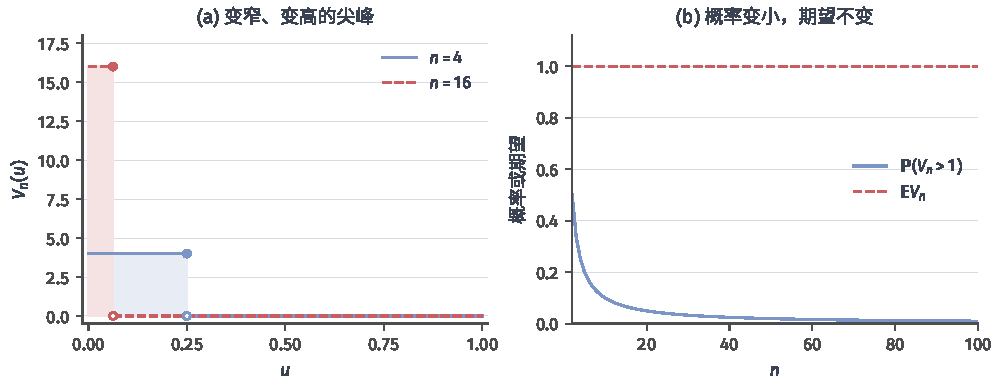
\includegraphics[width=\linewidth]{figures/01-mathematical-preliminaries/04-random-variables-distributions-and-causality/matplotlib/probability-vanishing-spikes/figure.pdf}
  \caption{小概率尖峰与期望质量（解析式教学图）。左图为\(V_n(u)=n\mathbb I\{u\leq1/n\}\)在\(n=4,16\)时的取值，均以面积\(1\)贡献期望；右图对\(n\geq2\)显示\(\mathbb P(V_n>1)=1/n\)趋于零，而\(\mathbb E V_n=1\)不变。基础变量为\(U\sim\operatorname{Unif}(0,1)\)。}
  \label{fig:probability-vanishing-spikes}
\end{figure*}
% Baseline T:500-512
渐近展开经常同时出现确定的缩放因子和随机余项。不能用“每次取值都有限”代替余项控制：所需的是坏事件的概率能被同一常数压小。概率阶记号把这种控制与确定数列的阶区分开。
\begin{definition}[概率阶记号]
  \label{def:statistics-probability-order}
\term{概率有界}（bounded in probability）把“随机量不会随\(n\)逃向无穷”写成
可检验的概率条件。若对每个\(\epsilon>0\)，都存在有限常数\(M\)和整数\(n_0\)，使
\[
  \sup_{n\geq n_0}\mathbb{P}(|X_n|>M)<\epsilon,
\]
就记\(X_n=O_{\mathbb{P}}(1)\)。若\(X_n\to_{\mathbb{P}}0\)，则记
\(X_n=o_{\mathbb{P}}(1)\)。对确定正数列\(a_n\)，约定\(X_n=O_{\mathbb P}(a_n)\)与\(X_n=o_{\mathbb P}(a_n)\)分别表示\(X_n/a_n=O_{\mathbb P}(1)\)与\(X_n/a_n=o_{\mathbb P}(1)\)。
\end{definition}
依分布收敛的序列必然概率有界，但
\(O_{\mathbb{P}}(1)\)本身不指定唯一极限分布。

\begin{theorem}[连续映射]
\label{thm:rv-continuous-mapping}
若\(X_n\to X\)几乎必然或依概率，且可测函数\(g\)在\(X\)的取值处几乎必然连续，则\(g(X_n)\to g(X)\)具有相应收敛方式。
若\(X_n\Rightarrow X\)且\(\mathbb P(X\in D_g)=0\)，其中\(D_g\)为\(g\)的不连续点集，则\(g(X_n)\Rightarrow g(X)\)。变量可取值于Polish空间。
\end{theorem}
\begin{proof}
几乎必然情形逐条在连续点应用确定序列的极限规则。依概率情形使用子列判据：每个子列都有一个几乎必然收敛的子子列，应用前一结论，再用同一判据返回依概率收敛。依分布情形对闭集\(C\)，有
\(\overline{g^{-1}(C)}\subseteq g^{-1}(C)\cup D_g\)；下一小节Portmanteau的闭集上界给出
\(\limsup_n\mathbb P(g(X_n)\in C)\leq\mathbb P(g(X)\in C)\)，即得结论。
\end{proof}
例如倒数映射在零不连续；只有极限以概率一非零时才可直接取倒数。均方收敛不能对任意连续函数自动传递，因为变换可能放大尾部。
% Baseline T:562-634
\begin{theorem}[Slutsky定理]
  \label{thm:statistics-slutsky}
  若\(X_n\xrightarrow{\mathrm d}X\)，且
  \(Y_n\xrightarrow{\mathbb{P}}c\)，其中\(c\)为常数，则
  \[
    X_n+Y_n\xrightarrow{\mathrm d}X+c,\qquad
    X_nY_n\xrightarrow{\mathrm d}cX.
  \]
  若\(c\neq0\)，还有
  \(X_n/Y_n\xrightarrow{\mathrm d}X/c\)。特别地，若
  \(R_n=o_{\mathbb{P}}(1)\)，则
  \(X_n+R_n\xrightarrow{\mathrm d}X\)。
\end{theorem}

Slutsky定理允许把收敛到常数的标准误、归一化因子或余项代入渐近分布。它不表示两个一般
随机极限可以忽略联合分布；关键条件是其中一个序列依概率收敛到常数。

\begin{theorem}[Delta方法]
\label{thm:statistics-delta-method}
若
\(\sqrt n(\widehat\theta_n-\theta)\xrightarrow{\mathrm d}\mathcal N(0,V)\)，
且\(g\)在\(\theta\)处可微，则
\[
  \sqrt n\bigl(g(\widehat\theta_n)-g(\theta)\bigr)
  \xrightarrow{\mathrm d}
  \mathcal N\bigl(0,g'(\theta)^2V\bigr).
\]
\end{theorem}

\begin{proof}
记
\[
  Z_n=\sqrt n(\widehat\theta_n-\theta),
  \qquad
  Z\sim\mathcal N(0,V).
\]
先补出证明所需的两条概率阶规则。由\(Z_n\xrightarrow{\mathrm d}Z\)，对任意
\(\epsilon>0\)，可取充分大的\(M\)使
\(\mathbb{P}(|Z|\geq M)<\epsilon/2\)。依分布收敛的闭集上界给出
\[
  \limsup_{n\to\infty}\mathbb{P}(|Z_n|\geq M)
  \leq \mathbb{P}(|Z|\geq M)<\epsilon/2,
\]
所以\(Z_n=O_{\mathbb{P}}(1)\)。此外，若
\(A_n=o_{\mathbb{P}}(1)\)、\(B_n=O_{\mathbb{P}}(1)\)，则对任意
\(\eta,\epsilon>0\)，先取\(M\)使大样本下
\(\mathbb{P}(|B_n|>M)<\epsilon/2\)，再取充分大的\(n\)使
\(\mathbb{P}(|A_n|>\eta/M)<\epsilon/2\)。于是
\[
  \mathbb{P}(|A_nB_n|>\eta)
  \leq
  \mathbb{P}(|B_n|>M)
  +\mathbb{P}(|A_n|>\eta/M)
  <\epsilon,
\]
即\(o_{\mathbb{P}}(1)O_{\mathbb{P}}(1)=o_{\mathbb{P}}(1)\)。

特别地，
\(\widehat\theta_n-\theta=n^{-1/2}Z_n=o_{\mathbb{P}}(1)\)，所以估计量依概率一致。
Taylor展开给出
\[
  g(\widehat\theta_n)-g(\theta)
  =g'(\theta)(\widehat\theta_n-\theta)
   +r_n(\widehat\theta_n-\theta),
\]
其中一致性与可微性保证\(r_n=o_{\mathbb{P}}(1)\)。乘以\(\sqrt n\)后，
余项是
\(r_nZ_n=o_{\mathbb{P}}(1)\)。主项由假设依分布收敛，再用Slutsky定理即得结论。
\end{proof}

例如若某估计量满足
\(\sqrt n(\widehat\theta_n-\theta)\Rightarrow\mathcal N(0,\sigma^2)\)，且
\(\theta>0\)，取\(g(\theta)=\log\theta\)，其渐近方差为
\(\sigma^2/\theta^2\)。估计量以趋于一的概率落在正半轴；在非正事件上任取一个约定值不影响极限。
若\(g'(\theta)=0\)，一阶Delta方法仍成立，但只给出零方差的退化极限；要描述非退化波动，需要更高阶展开与新的缩放。若\(g\)在目标点不可微，才不能直接应用上述定理。

\subsubsection{概率分布的弱收敛}
\label{sec:rv-weak-convergence}
此前的依分布收敛比较数值随机结果。路径、随机向量和最优传输中的联合分布也需要同一种比较，但未必共用基础概率空间。此时直接比较概率测度，比寻找逐点对应更自然。

\begin{definition}[概率测度的弱收敛]
\label{def:information-weak-measure-convergence}
对同一度量空间上的Borel概率测度\(P_n,P\)，若对每个有界连续实函数\(h\)均有
\(\int h\,\mathrm dP_n\to\int h\,\mathrm dP\)，就称\(P_n\)弱收敛到\(P\)，记作\(P_n\Rightarrow P\)。这种\term{概率测度的弱收敛}（weak convergence of probability measures）只比较各测度的积分，不要求随机变量在同一基础空间上逐点接近。
\end{definition}
有界连续函数是比较分布的探针：连续性不放大微小位置移动，有界性不让极少量远处质量主导结果。实数上的这个定义等价于在\(F\)的全部连续点上有\(F_n(x)\to F(x)\)，也就与随机变量的依分布收敛一致。例如\(\delta_{1/n}\Rightarrow\delta_0\)，但对集合\(\{0\}\)，前者始终赋概率零、后者赋概率一；弱收敛不要求每个事件的概率都收敛。

\begin{theorem}[Portmanteau的常用形式]
\label{thm:rv-portmanteau}
在Polish空间\(E\)上，Borel概率测度\(P_n\Rightarrow P\)等价于下列任一条件：
对每个闭集\(C\)，\(\limsup_nP_n(C)\leq P(C)\)；
对每个开集\(G\)，\(\liminf_nP_n(G)\geq P(G)\)；
对每个满足\(P(\partial A)=0\)的Borel集\(A\)，\(P_n(A)\to P(A)\)。
弱收敛还给出每个非负下半连续函数\(c\)的积分下界
\[
\int c\,\mathrm dP\leq\liminf_n\int c\,\mathrm dP_n.
\]
\end{theorem}
这里Polish指拓扑可由完备可分度量诱导。闭集条件可由连续函数
\(h_k(x)=\max\{1-k\,d(x,C),0\}\)从上逼近\(\mathbb I_C\)得到，开集条件再取补集。若边界质量为零，对内部和闭包夹逼即得事件概率收敛。非负下半连续函数可由递增的有界连续函数逼近，先对每个逼近函数取弱极限，再用单调收敛，得到积分不等式。这也解释了为何非负成本的极限只能先得到下界；无界一般函数需要额外的尾部控制。

弱收敛的另一困难是质量可能不断远移，使任何候选极限都留不住总概率。需要紧性把绝大部分质量统一留在可控区域。
\begin{definition}[紧概率测度与一致紧族]
\label{def:information-tightness}
度量空间上的Borel概率测度\(P\)称为\term{紧的}，若对每个
\(\varepsilon>0\)存在紧集\(K\)，使\(P(K^{\mathsf c})<\varepsilon\)。
一族概率测度\(\mathcal P\)称为\term{一致紧的}，若对每个\(\varepsilon>0\)可取同一个紧集，使
\(\sup_{Q\in\mathcal P}Q(K^{\mathsf c})<\varepsilon\)。
\end{definition}
\begin{theorem}[Prokhorov定理]
\label{thm:rv-prokhorov}
Polish空间上的Borel概率测度族一致紧，当且仅当它相对弱序列紧，即每个序列都能抽出弱收敛到该空间上某个概率测度的子列。每个单独的Borel概率测度都是紧的。
\end{theorem}
定理保证可抽取子列，不保证所有子列具有同一极限；还需识别极限才能证明整列收敛。单个测度紧也不等于一个族一致紧。例如\(\{\delta_n:n\geq1\}\)的每个成员都紧，但任何固定紧集只能留住有限多个点，整个族不一致紧。

在\(\mathbb R^d\)中，若\(\sup_n\mathbb E\|X_n\|^p\leq C<\infty\)，其中\(p>0\)，则
\[
\sup_n\mathbb P(\|X_n\|>R)\leq C/R^p.
\]
闭球紧，故这些分布一致紧。在一般无限维空间，闭有界集未必紧，单有范数矩界不能照搬此论证。后面路径收敛还需控制短时间内的振荡；
“随机分布”章的第~\ref{sec:information-optimal-coupling-existence}节
则在固定边缘下构造共同紧集。二者都使用本节的通用定义，不是固定测度下的积分交换。

\subsubsection{聚合结果的极限规律}
\label{sec:rv-aggregate-limits}
% Baseline P:1448-1511
\begin{theorem}[强大数定律]
\label{thm:probability-strong-law-large-numbers}
若\(X_1,X_2,\ldots\)独立同分布，且\(\mathbb{E}[|X_1|]<\infty\)，则
\[ \overline{X}_n
  =\frac{1}{n}\sum_{i=1}^{n}X_i\to_{\mathrm{a.s.}}\mathbb{E}[X_1]. \]
\end{theorem}

强大数定律说明同一分布下的独立重复观测，其平均几乎必然接近期望。有限方差是许多初等证明使用的方便条件，但独立同分布版本的结论只需有限一阶绝对矩。若观测相关、分布随
时间变化或样本由自适应规则收集，则不能直接引用该定理；第~\ref{sec:stoch-markov-long-run-average}节给出相关过程的一组替代条件
\scite{math-kallenberg2021probability}

有限方差时，较弱的依概率结论可以在这里完整得到。若
\(\operatorname{Var}(X_1)=\sigma^2<\infty\)，独立性使
\[
  \operatorname{Var}(\overline{X}_n)
  =\frac{1}{n^2}\sum_{i=1}^{n}\operatorname{Var}(X_i)
  =\frac{\sigma^2}{n}.
\]
把式~\eqref{eq:probability-chebyshev-inequality}用于样本平均，有
\[
  \mathbb{P}\bigl(
    |\overline{X}_n-\mathbb{E}X_1|\geq\varepsilon
  \bigr)
  \leq\frac{\sigma^2}{n\varepsilon^2}\to0.
\]
这证明了有限方差版本的弱大数定律。强大数定律只要求有限一阶绝对矩，但其证明还需截断大取值、控制截断变量的独立和，并把可求和坏事件转成几乎必然结论；不能由上面的逐个\(n\)概率界直接推出。

对例~\ref{ex:probability-noisy-observation}中的独立同分布噪声，只要\(\mathbb{E}|\varepsilon_i|<\infty\)，便有
\[ \overline{Y}_n
  =\theta+\frac{1}{n}\sum_{i=1}^{n}\varepsilon_i\to_{\mathrm{a.s.}}\theta. \]
这回答了“多测几次再平均是否稳定”，但没有给出固定\(n\)时误差超过指定阈值的概率。

\par\medskip\noindent\textbf{中心极限定理与缩放波动}\quad
\begin{theorem}[Lindeberg--L\'evy中心极限定理]
\label{thm:probability-iid-central-limit}
若\(X_1,X_2,\ldots\)独立同分布，\(\mathbb{E}X_1=\mu\)，\(0<\operatorname{Var}(X_1)=\sigma^2<\infty\)，则
\[ \frac{\sqrt{n}(\overline{X}_n-\mu)}{\sigma}
  \Rightarrow\mathcal{N}(0,1). \]
\end{theorem}

大数定律研究未缩放误差是否趋于零，中心极限定理研究乘以\(\sqrt{n}\)后的剩余波动近似什么分布。它给出渐近近似，而不是每个有限\(n\)都精确服从高斯分布。若方差
无限、样本依赖过强或分布随\(n\)变化而不满足相应Lindeberg条件，\(\sqrt{n}\)缩放与高斯极限都可能失效。

证明的关键是特征函数。令\(Y_i=(X_i-\mu)/\sigma\)，并记
\(\varphi(t)=\mathbb{E}e^{\mathrm{i}tY_1}\)。复指数绝对值恒为\(1\)，所以特征函数总有定义。由
\(\mathbb{E}Y_1=0\)、\(\mathbb{E}Y_1^2=1\)及零点处的二阶展开，
\[
  \varphi(u)=1-\frac{u^2}{2}+o(u^2),
  \qquad u\to0.
\]
独立性使标准化和的特征函数分解为
\[
  \mathbb{E}\exp\left\{
    \mathrm{i}t\frac{1}{\sqrt n}\sum_{i=1}^{n}Y_i
  \right\}
  =
  \left[\varphi\left(\frac{t}{\sqrt n}\right)\right]^n
  \longrightarrow e^{-t^2/2}.
\]
右侧是标准高斯的特征函数，并且在零点连续。定理
~\ref{thm:probability-levy-continuity}于是给出依分布收敛。第
~\ref{sec:statistics-intervals-quantiles}节会用这个渐近分布构造近似区间，但有限样本覆盖
仍需额外误差控制，不能只引用极限式。
现在可以回到第~\ref{sec:probability-monte-carlo-variance-reduction}节，逐项核验积分近似的长期条件。直接平均只要
\(\mathbb E|f(X)|<\infty\)就强一致，若再有有限正方差，则中心极限定理给出
\(\sqrt n(\widehat I_n-I)\Rightarrow\mathcal N(0,\operatorname{Var}(f(X)))\)。
重要性采样把\(f(X)\)换成\(w(X)f(X)\)，因此要在来源分布下分别查
\(\mathbb E|wf|\)和\(\mathbb E[(wf)^2]\)；密度比存在并不推出第二项有限。

控制变量使用预先固定的系数及已知均值时，同样对修正后的被积量检查一阶、二阶矩。若系数由同一数据估计，无偏性可能不再成立；在系数一致、控制变量有适当矩等条件下，可用Slutsky分析其余项，不能直接照搬固定系数公式。Rao--Blackwell化的条件期望保留一阶可积性，在二阶可积时又由条件Jensen不等式不增方差。

自归一化重要性估计是两个平均的比。设非归一化权重\(\widetilde w\geq0\)，
\(0<Z=\mathbb E_Q\widetilde w<\infty\)，且
\(\mathbb E_Q|\widetilde wf|<\infty\)。沿用\(\widetilde w/Z=\mathrm dP/\mathrm dQ\)
及独立同分布的\(Q\)样本，两个强大数定律和连续映射给出
\[
\frac{\sum_i\widetilde w(X_i)f(X_i)}
{\sum_i\widetilde w(X_i)}
\longrightarrow
\frac{\mathbb E_Q[\widetilde wf]}Z=I
\quad\text{几乎必然}.
\]
分母由强大数定律最终远离零。若
\(\mathbb E_Q[\widetilde w^2(1+f^2)]<\infty\)，可把中心化比值直接写成
\[
 \sqrt n(\widehat I_{\mathrm{SN}}-I)
 =\frac{n^{-1/2}\sum_{i=1}^n
       \widetilde w(X_i)(f(X_i)-I)}
       {n^{-1}\sum_{i=1}^n\widetilde w(X_i)}.
\]
分子的求和项独立同分布，均值为零，方差为
\(\mathbb E_Q[\widetilde w^2(f-I)^2]\)。方差为正时，标量中心极限定理给出分子的高斯极限；分母强收敛到\(Z>0\)，再用Slutsky定理，得到渐近方差
\[
\frac{\mathbb E_Q[\widetilde w^2(f-I)^2]}{Z^2}.
\]
若该方差为零，分子各项几乎必然为零，极限相应退化为零常量。
这没有消除有限样本比值偏差。固定阈值截断权重通常收敛到截断后的目标；若希望阈值随样本量增长而仍恢复原积分，还要证明被截去尾部和随机误差同时消失。

\subsection{从随机序列到随机过程}
\label{sec:stoch-process-joint-laws}
序列已经能表达离散轮次；连续时间还包含不可数多个时刻。一条路径上的正则性因而不能由逐点边缘条件替代。

\subsubsection{时间索引与样本路径}
\label{sec:rv-paths}
% Baseline S:32-36
一个随机变量描述一次结果；要研究多次观测如何关联，必须把它们放到同一个概率空间上。
\begin{definition}[随机过程]
  \label{def:stoch-process}
  给定概率空间\((\Omega,\mathcal F,\mathbb P)\)、索引集\(T\)和状态可测空间\((\mathcal X,\mathcal A)\)，\term{随机过程}（stochastic process）是一族随机变量\((X_t)_{t\in T}\)，其中每个\(X_t:\Omega\to\mathcal X\)均可测。
\end{definition}
离散时间通常取\(T=\mathbb N_0\)，连续时间取\(T=[0,\infty)\)。固定时刻\(t\)，
\(\omega\mapsto X_t(\omega)\)是随机变量；固定基础结果\(\omega\)，
\(t\mapsto X_t(\omega)\)是样本路径。所谓连续时间只规定索引可以任取实数，不规定取值连续，更不规定路径连续。

图~\ref{fig:rv-paths}中，沿横轴看一条线，是一次实现随时间怎样变化；沿竖线看多个交点，是同一时刻在不同实现中的结果。右连续阶梯路径可以在连续时间定义却只取整数；连续实值路径也可能非常粗糙。稍后的Poisson和Brownian过程分别给出这两种情形的正式模型。
\begin{figure}[htbp]
  \centering
  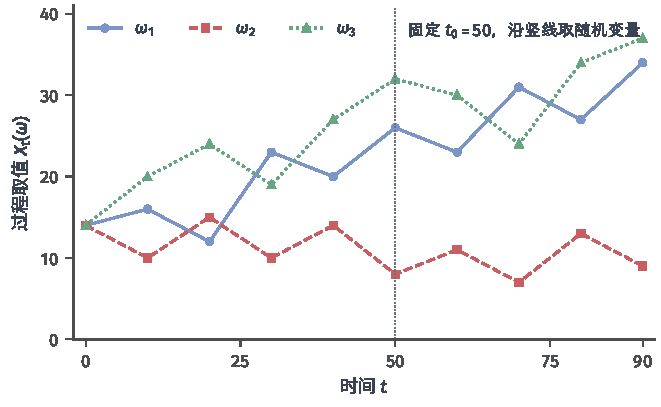
\includegraphics[width=\linewidth]{figures/01-mathematical-preliminaries/04-random-variables-distributions-and-causality/matplotlib/rv-paths/figure.pdf}
  \caption{同一过程的路径与时刻截面是不同对象。图为人为给定的三条示意路径，竖虚线固定时刻\(t_0\)；交点展示该时刻可能出现的不同值，并非用三条路径估计出的概率密度。}
\label{fig:rv-paths}
\end{figure}

\subsubsection{有限维分布与过程规律}
\label{sec:rv-finite-dimensional-laws}
给定各个有限时刻集合上的联合分布，当前要检查它们能否来自同一个过程。
构造出过程以后，还要检查能否选择连续路径的版本；比较一列近似过程时，则要
检查整条路径是否收敛。这三个问题分别涉及过程的存在、路径的正则性与近似过程的
极限，不能由单个时刻的分布一并回答。

只给每个时刻的边缘分布，无法判断相邻时刻是同向、独立还是反向变化。有限维分布是在任意有限时刻集合上给出
\(\mathcal L(X_{t_1},\ldots,X_{t_m})\)，把这种共同变化也保存下来。

要把这些有限观测放到同一个空间中，记\(E^T\)为全部映射\(x:T\to E\)的集合。
其乘积\(\sigma\)代数由有限坐标柱集生成；这类集合的形式是
\[
 \{x\in E^T:(x(t_1),\ldots,x(t_m))\in B\},
\]
其中\(B\)为有限积\(E^m\)中的可测集。它只检查有限个坐标是否满足某项条件，再由可数集合运算生成更多事件；每个坐标评价\(x\mapsto x(t)\)因此可测。

\begin{theorem}[Kolmogorov扩张的标准Borel版本]
\label{thm:rv-kolmogorov-extension}
设状态空间\(E\)是标准Borel空间，\(T\)为任意索引集。若给定每个有限索引集合\(J\subset T\)上的概率测度\(P_J\)，且对有限集合\(J\subset K\)，从\(E^K\)投影到\(E^J\)把\(P_K\)推送为\(P_J\)，则存在唯一的概率测度定义在\(E^T\)的乘积\(\sigma\)代数上，使各坐标过程具有这些有限维分布。
用有序时刻元组表示时，还必须满足重排坐标的相容性。
\end{theorem}
相容性意味着同一个两时刻问题，不论直接指定还是从三时刻问题删掉一个坐标，都应得到同一答案。高斯过程的半正定核会提供一组相容的高斯向量，因而可用此定理建立过程。扩张定理不同时承诺它落在连续路径空间中，也不保证
\((t,\omega)\mapsto X_t(\omega)\)联合可测。这里的唯一性只针对乘积\(\sigma\)代数中的事件；整条路径的连续性还须另行建立版本及适合的路径空间。

若对每个固定\(t\)，\(\mathbb P(X_t=Y_t)=1\)，称\(X,Y\)互为版本；若
\(\mathbb P(\forall t,\ X_t=Y_t)=1\)，则称不可区分。不可数时间集上，两者不同。
例如\(U\)在\([0,1]\)均匀分布，\(X_t=\mathbb I_{\{t=U\}}\)、\(Y_t=0\)：
每个固定时刻两者几乎必然相等，但每条\(X\)路径都在某个时刻出现尖点。
若两个版本都具有右连续路径，则先在可数稠密时刻同时相等，再用右连续性推广，才得到不可区分。

描述连续路径的粗糙程度时，称\(x\)在紧时间区间上具有正指数\(\alpha\)的Hölder连续性，是指存在有限\(C_x\)，使
\[
 |x(t)-x(s)|\leq C_x|t-s|^\alpha
 \quad\text{对区间内所有 }s,t\text{成立}.
\]
随机路径允许常数\(C_x\)依赖具体实现。\(\alpha=1\)就是Lipschitz条件；在短时间差上，较小的正指数给出较弱的约束。例如\(\sqrt t\)满足
\(|\sqrt t-\sqrt s|\leq|t-s|^{1/2}\)，却在零点附近不满足Lipschitz条件。这里是路径正则性，与同名的Hölder积分不等式不同。

得到连续版本的一项常用充分条件是Kolmogorov连续性准则：若在紧时间区间上存在
\(p>0,\beta>0,C<\infty\)，使
\[
\mathbb E|X_t-X_s|^p\leq C|t-s|^{1+\beta},
\]
则存在连续版本，并可取得任意小于\(\beta/p\)的正Hölder指数；该条件本身不保证达到端点\(\beta/p\)。条件控制的是整族短时增量，不能由每个时刻分布连续推出。对Brownian增量，四阶矩为\(3|t-s|^2\)，足以给出连续版本；更高阶矩可把Hölder指数推进到任意小于\(1/2\)。

\subsubsection{随机路径的收敛条件}
\label{sec:rv-path-convergence}
前面讨论同一个过程是否有连续版本；现在比较的是一列过程及其极限。路径极限
把整条函数当成随机对象，必须先规定函数之间怎样接近。对实值连续路径，
\(C([0,T])\)取一致距离
\(\|x-y\|_\infty=\sup_{t\leq T}|x(t)-y(t)|\)，是Polish空间。
对右连续且有左极限的路径，使用\(D([0,T])\)及Skorokhod \(J_1\)拓扑：
若存在严格递增的连续双射\(\lambda_n:[0,T]\to[0,T]\)，使
\[
\|\lambda_n-\operatorname{id}\|_\infty\to0,\qquad
\|x_n\circ\lambda_n-x\|_\infty\to0,
\]
就有\(x_n\to x\)于该拓扑。它允许跳跃时刻略微错开，再对齐比较；相应拓扑可由完备可分度量刻画。若极限连续，\(J_1\)收敛等价于一致收敛。

有限维收敛仍不够。取确定连续函数
\[
x_n(t)=\max\{1-n^2|t-1/n|,0\},\qquad 0\leq t\leq1,\ n\geq2.
\]
每个固定时刻最终避开窄尖峰，所以任意有限维向量趋零；但
\(\|x_n\|_\infty=1\)，不可能在\(C([0,1])\)中趋零。
越来越窄的尖峰没有被有限个截面发现，却阻止了路径规律的紧性。

\begin{theorem}[连续路径的紧性与极限识别]
\label{thm:rv-continuous-path-tightness}
设\(X_n\)是\(C([0,T])\)值随机对象。令
\[
w(x,\delta)=\sup_{\substack{s,t\in[0,T]\\|t-s|\leq\delta}}|x(t)-x(s)|.
\]
若\((X_n(0))\)的分布一致紧，且对每个\(\varepsilon>0\)，
\[
\lim_{\delta\downarrow0}\sup_n
\mathbb P\{w(X_n,\delta)>\varepsilon\}=0,
\]
则路径分布一致紧。若其有限维分布还收敛到某个连续过程\(X\)的有限维分布，则
\(X_n\Rightarrow X\)于\(C([0,T])\)。
\end{theorem}
这里用到Arzelà--Ascoli定理的确定性形式：紧区间上一族连续函数若统一有界且等度连续，其一致范数闭包就是紧集。等度连续指对每个误差阈值，都能选择同一个时间间隔，同时控制族内全部函数的短时变化；每个函数各自连续还不够。该紧性定理的证明见实分析教材\scite{math-folland1999real}

为把概率条件对应到这两项要求，固定\(0<\epsilon<1\)。由初值一致紧选\(M<\infty\)，使
\(\sup_n\mathbb P(|X_n(0)|>M)\leq\epsilon/2\)。
再取\(\eta_k=2^{-k}\)，逐个选取递减的\(\delta_k\downarrow0\)，使
\[
 \sup_n\mathbb P\{w(X_n,\delta_k)>\eta_k\}
 \leq\epsilon\,2^{-k-1},\qquad k\geq1.
\]
联合界说明每条\(X_n\)以至少\(1-\epsilon\)的概率同时满足初值界和全部尺度的振荡界。
满足这些限制的确定性路径族等度连续；把\([0,T]\)分成有限个长度不超过\(\delta_1\)的小段，还得到统一幅度界
\(M+\lceil T/\delta_1\rceil\eta_1\)。
因此其闭包是承载至少\(1-\epsilon\)概率的紧集，得到所需路径分布的一致紧性。

Prokhorov定理给出子列极限，坐标评价在\(C\)中连续，因此有限维规律识别每个子列极限。连续路径的Borel规律由稠密时刻坐标决定，故所有子列指向同一个极限。
若连续\(X_n\)满足统一矩界
\(\mathbb E|X_n(t)-X_n(s)|^p\leq C|t-s|^{1+\beta}\)，且初值一致紧，则是上述模连续性条件的一项常用充分条件。

跳跃路径不能使用同一个连续模量：一个合法跳跃已使其无法趋零。对
\(D\)空间须另证\(J_1\)紧性，再在极限几乎必然连续的时刻核对有限维收敛。例如可用有界时间内的紧包含条件及停时短增量条件建立紧性；这些是额外假设，不由单时刻收敛自动成立。

缩放随机游走给出重要入口。若\(\xi_i\)独立同分布、均值零、方差一，
令\(S_k=\sum_{i=1}^k\xi_i\)，在网格\(k/n\)上取\(S_k/\sqrt n\)并作线性插值。
Donsker定理说明这些随机折线在\(C([0,T])\)中弱收敛到标准Brownian运动。
阶梯插值相应在\(D\)的\(J_1\)拓扑收敛。这里同时需要有限维极限与路径紧性，不能只把单时刻中心极限定理改写成带\(t\)的公式；Brownian的完整定义见第~\ref{sec:dynamical-brownian-motion}节。

\subsection{随机过程中的依赖结构}
\label{sec:stoch-martingales-stopping-sequential-concentration}
未来可以依赖历史，但要说清依赖的哪一部分。Markov关系约束完整条件分布，鞅关系只约束条件均值，平稳性则比较时间平移前后的联合规律。共同的准备是把“已经知道什么”写成一个逐渐增加的信息族。
% Baseline S:371-384
\begin{definition}[滤过、适应与可预测性]
  \label{def:stoch-filtration-adaptation-predictability}
在概率空间
$(\Omega,\mathcal{F},\mathbb{P})$上，令每个$\mathcal{F}_t$都是
$\mathcal{F}$的子$\sigma$代数，并且
\[
  \mathcal{F}_0\subseteq\mathcal{F}_1\subseteq\cdots\subseteq\mathcal{F}.
\]
这列递增的子$\sigma$代数称为\term{滤过}（filtration），可以理解为随时间增长的信息。
随机变量$X_t$若对
$\mathcal{F}_t$可测，就称它在时刻$t$已经可知；若每个$t$都如此，称$(X_t)$适应于该滤过。对$t\geq1$，过程$(H_t)$若$H_t$对
$\mathcal{F}_{t-1}$可测，就称为\term{可预测过程}（predictable process）。
\end{definition}
这里的“可预测”不是说$H_t$没有随机性，而是说它可以由第$t$次新噪声到来之前的信息确定。
% Baseline S:441-447
\begin{definition}[停时]
  \label{def:stoch-stopping-time}
  相对于滤过\((\mathcal F_t)_{t\geq0}\)，取值于\(\mathbb N_0\cup\{\infty\}\)的随机时刻$\tau$若满足$\{\tau\leq t\}\in\mathcal{F}_t$对每个整数$t\geq0$成立，就称为\term{停时}（stopping time）。
\end{definition}
到时刻$t$为止已有的信息足以判断是否已经停止；“最后一次
达到最大值的时刻”通常需要看到未来，不一定是停时。


\subsubsection{Markov条件分布关系}
\label{sec:rv-markov}
% Baseline S:69-131
\begin{definition}[Markov链]
  \label{def:stoch-markov-chain}
设$(Z_t)_{t\geq0}$取值于可测空间$(\mathcal{Z},\mathcal{A})$。若对每个
$B\in\mathcal{A}$，
\[
  \mathbb{P}(Z_{t+1}\in B\mid Z_0,\ldots,Z_t)
  =
  \mathbb{P}(Z_{t+1}\in B\mid Z_t),
\]
则称$(Z_t)$为\term{Markov链}（Markov chain）；上述条件等式按几乎必然意义理解。
\end{definition}
这个条件不是说过去没有影响，而是
说当前状态已经保存了预测下一步所需的全部历史信息。
\begin{definition}[时间齐次Markov链]
  \label{def:stoch-time-homogeneous-chain}
  若存在从\((\mathcal Z,\mathcal A)\)到自身的概率核\(P\)，使所有\(t\geq0\)、\(B\in\mathcal A\)都满足
  \[ \mathbb P(Z_{t+1}\in B\mid Z_t)=P(Z_t,B)\quad\text{几乎必然}, \]
  则该Markov链称为\term{时间齐次的}（time-homogeneous）。
\end{definition}
时间齐次描述机制不变，不代表$Z_t$的边缘分布不随时间改变
\scite{math-meyn2009markov}

概率核的两项要求见定义~\ref{def:probability-kernel}：每个状态对应合法的下一步分布，而每个事件的概率随当前状态可测地变化。对有界可测函数$f$，记
\[
  Pf(z)=\int_{\mathcal{Z}}f(z')P(z,\mathrm{d}z').
\]
两个核的复合按
\[
  (PQ)(z,B)
  =
  \int_{\mathcal{Z}}Q(z',B)P(z,\mathrm{d}z')
\]
定义；它表示先按$P$走一步，再按$Q$走一步。令$P^0(z,B)=\mathbb{I}\{z\in B\}$，
$P^{m+1}=P^mP$，则时间齐次链满足
\begin{equation}
  \mathbb{P}(Z_{t+m}\in B\mid Z_t=z)=P^m(z,B),
  \qquad
  P^{m+n}(z,B)
  =
  \int_{\mathcal{Z}}P^n(z',B)P^m(z,\mathrm{d}z').
  \label{eq:stoch-chapman-kolmogorov}
\end{equation}
第二个等式称为\term{Chapman--Kolmogorov关系}。证明可直接使用条件概率的塔式性质：
给定$Z_{t+m}=z'$后，Markov性质把后$n$步的条件概率化为$P^n(z',B)$；再对
$Z_{t+m}$在给定$Z_t=z$时的分布$P^m(z,\mathrm{d}z')$积分，就得到右侧。取$n=1$
并归纳，还同时证明了第一个等式及核幂确实给出多步转移。

\begin{definition}[平稳分布]
  \label{def:stoch-stationary-distribution}
概率分布$\pi$若满足
\begin{equation}
  \pi(B)=\int_{\mathcal{Z}}P(z,B)\,\pi(\mathrm{d}z),
  \qquad B\in\mathcal{A},
  \label{eq:stoch-stationary-distribution}
\end{equation}
就称为$P$的\term{平稳分布}（stationary distribution）。
\end{definition}
若$Z_0\sim\pi$，式
\eqref{eq:stoch-stationary-distribution}保证每个$Z_t$仍服从$\pi$；若从指定状态
$z_0$启动，平稳性本身却没有说明$\mathcal{L}(Z_t)$会趋向$\pi$。恒等转移核
$P(z,B)=\mathbb{I}\{z\in B\}$保持任意分布，但它永远不忘记初态，这已经表明“保持
目标”和“到达目标”是两项不同要求。

% Baseline S:151-163
\begin{definition}[细致平衡]
  \label{def:stoch-detailed-balance}
概率核\(P\)与概率测度\(\pi\)满足\term{细致平衡}（detailed balance），若以下两个联合测度在\(\mathcal Z\times\mathcal Z\)上相同：
\begin{equation}
  \pi(\mathrm{d}z)P(z,\mathrm{d}z')
  =\pi(\mathrm{d}z')P(z',\mathrm{d}z).
  \label{eq:stoch-detailed-balance}
\end{equation}
\end{definition}
它要求平稳运行时任意两处之间的概率流量正反相等。对$z$积分便得到
\eqref{eq:stoch-stationary-distribution}，所以细致平衡足以推出平稳性。反向不成立：
围绕三个状态单向循环的链可以保持均匀分布，却没有逐边对称的反向流。细致平衡是构造
采样链的便利证书，不是遍历平均成立的必要定义。
% Baseline P:1257-1273
换测度也可作用于整段观测，而不只作用于一个随机变量。考虑长度\(T\)的轨迹
\(\tau=(s_0,a_0,s_1,a_1,\ldots,s_T)\)，其中\(s_t\)记录当前状态，\(a_t\)记录当步行动。
假定行动只按当前状态的概率核\(\pi(a_t\mid s_t)\)产生，下一状态只按
\(P(s_{t+1}\mid s_t,a_t)\)产生，且这两个核不随时间改变。
初始分布为\(\rho\)时，条件概率的链式分解给出
\[ p_\pi(\tau)
  =\rho(s_0)\prod_{t=0}^{T-1}\pi(a_t\mid s_t)P(s_{t+1}\mid s_t,a_t). \]
若目标策略为\(\pi\)，采样策略为\(\mu\)，并且两者共享同一初始分布和环境转移核，公共因子相消，得到
\begin{equation}
  \frac{p_\pi(\tau)}{p_\mu(\tau)}
  =
  \prod_{t=0}^{T-1}
  \frac{\pi(a_t\mid s_t)}{\mu(a_t\mid s_t)}.
  \label{eq:probability-trajectory-likelihood-ratio}
\end{equation}
该公式要求目标轨迹分布绝对连续于采样轨迹分布。具体地说，只要\(\pi(a\mid s)>0\)，在可能到达的状态上就需要\(\mu(a\mid s)>0\)。共同环境假设若不成立，转移核的比值也必须保留。即使每一步
比值有限，长轨迹连乘仍可能产生极大方差；密度比存在并不提供可用的二阶误差界。

\subsubsection{鞅条件均值关系}
\label{sec:rv-martingales}
% Baseline S:386-425
\begin{definition}[鞅与鞅差]
  \label{def:stoch-martingale}
可积过程$(M_t)$若适应于$(\mathcal{F}_t)$，并满足
\begin{equation}
  \mathbb{E}[M_t\mid\mathcal{F}_{t-1}]=M_{t-1},
  \label{eq:stoch-martingale-definition}
\end{equation}
就称为\term{鞅}（martingale）。增量$X_t=M_t-M_{t-1}$满足
\begin{equation}
  \mathbb{E}[X_t\mid\mathcal{F}_{t-1}]=0,
  \label{eq:stoch-martingale-difference}
\end{equation}
称为\term{鞅差}（martingale difference）。若条件等式改为\(\mathbb E[M_t\mid\mathcal F_{t-1}]\leq M_{t-1}\)，称\((M_t)\)为超鞅；改为\(\geq\)时称为次鞅。两者也要求每个时刻可积且适应。
\end{definition}
这里的\(t\)是离散整数时刻。连续时间的定义把相邻时刻条件换成：
对任意\(0\leq s\leq t\)，
\(\mathbb E[M_t\mid\mathcal F_s]=M_s\)几乎必然；每个时刻仍须可积且适应。
超鞅与次鞅分别改用\(\leq\)和\(\geq\)。后面的补偿计数与布朗运动均使用这一连续时间版本。
无条件零均值不够：若$X_t$可以由过去
预测，累计和仍可能形成系统漂移；式~\eqref{eq:stoch-martingale-difference}排除的正是
这种可利用的条件平均。

\begin{example}[公平随机游走与按过去下注]
  \label{ex:stoch-predictable-betting}
  设$\varepsilon_t$独立取$\{-1,1\}$，两种取值概率均为$1/2$，并令
  $\mathcal{F}_t=\sigma(\varepsilon_1,\ldots,\varepsilon_t)$。公平随机游走
  $S_t=\sum_{s=1}^{t}\varepsilon_s$是鞅。

  现在允许下注额$H_t$根据过去结果选择，只要求$H_t$对
  $\mathcal{F}_{t-1}$可测，并使$H_t\varepsilon_t$可积。财富过程
  \[
    M_t=M_0+\sum_{s=1}^{t}H_s\varepsilon_s
  \]
  仍是鞅，因为
  \[
    \mathbb{E}[H_t\varepsilon_t\mid\mathcal{F}_{t-1}]
    =
    H_t\mathbb{E}[\varepsilon_t\mid\mathcal{F}_{t-1}]
    =0.
  \]
  策略可以追涨、反向或在某些历史后停止下注，但只要它不能偷看$\varepsilon_t$，就不能
  改变下一笔收益的条件均值。若$H_t$依赖当前尚未揭晓的$\varepsilon_t$，上面的等式便
  失去依据。
\end{example}
% Baseline S:650-675

鞅关系约束每一步的条件均值，但是否存在长期极限仍需条件。非负超鞅的上穿论证给出一个基本结论。设$(L_t)$为非负超鞅且
$\mathbb{E}L_0<\infty$。对任意有理数$0<a<b$，记$U_n[a,b]$为
$L_0,\ldots,L_n$从不高于$a$到不低于$b$的完整上穿次数。在每次不高于$a$时持有一单位
过程、达到$b$时卖出；由于$(L_t)$是超鞅，这个可预测交易策略的期望收益不大于$0$。
比较每次完整交易至少$b-a$的路径收益与最后一次未完成交易，得到Doob上穿不等式
\[
  (b-a)U_n[a,b]
  \leq
  \text{交易收益}+(L_n-a)^-,
  \qquad x^-:=\max\{-x,0\}.
\]
其中负部$(L_n-a)^-$至多为$a$，而交易收益的期望不大于$0$。取期望得到
\[
  (b-a)\mathbb{E}U_n[a,b]
  \leq
  \mathbb{E}(L_n-a)^-
  \leq
  a.
\]
令$n\to\infty$可知每个正有理区间几乎必然只被上穿有限次。若$L_t$的下极限严格小于上
极限，就能在二者之间选到一个正有理区间并产生无穷多次上穿，形成矛盾。因此$L_t$几乎必然
存在扩展实数极限；再由Fatou引理与
$\sup_t\mathbb{E}L_t\leq\mathbb{E}L_0<\infty$排除极限为正无穷。于是非负超鞅几乎
必然收敛到有限随机变量。这个结论只保证路径极限存在；若还要交换极限与期望，仍需一致
可积等额外条件。
非负性不是鞅收敛的唯一入口。对有正有负的累计误差，常能控制的是二阶矩。
\begin{theorem}[二阶矩有界鞅的收敛]
\label{thm:rv-l2-martingale-convergence}
若\((M_n,\mathcal F_n)\)是平方可积鞅且
\(\sup_n\mathbb E M_n^2<\infty\)，则存在\(M_\infty\in L^2\)，使
\(M_n\to M_\infty\)几乎必然且在\(L^2\)中成立，并且
\(M_n=\mathbb E[M_\infty\mid\mathcal F_n]\)。
\end{theorem}
\begin{proof}
对\(m\geq n\)，条件均值性质给出
\(\mathbb E[M_n(M_m-M_n)]=0\)，所以
\[
\mathbb E(M_m-M_n)^2=\mathbb EM_m^2-\mathbb EM_n^2.
\]
右侧来自单调有界数列，故\(M_n\)在\(L^2\)中Cauchy，有\(L^2\)极限\(M_\infty\)。
还需将均方极限提升到整条序列的几乎必然极限。对有限鞅\(Y_j\)及
\(Y^*=\max_{j\leq N}|Y_j|\)，按首次越过水平\(a\)的时刻分解事件，并用
\(|Y_j|\leq\mathbb E[|Y_N|\mid\mathcal F_j]\)，得
\[
a\,\mathbb P(Y^*\geq a)
\leq\mathbb E[|Y_N|\mathbb I_{\{Y^*\geq a\}}].
\]
积分并用Cauchy--Schwarz，得到
\(\mathbb E(Y^*)^2\leq2\mathbb E(|Y_N|Y^*)\leq
2\|Y_N\|_2\|Y^*\|_2\)，故
\(\mathbb E(Y^*)^2\leq4\mathbb E Y_N^2\)。
把它用于从\(n\)起的差鞅，再令有限终点趋于无穷，有
\[
\mathbb P\left\{\sup_{m\geq n}|M_m-M_n|>\varepsilon\right\}
\leq\frac4{\varepsilon^2}
\bigl(\mathbb EM_\infty^2-\mathbb EM_n^2\bigr).
\]
取子列\(n_k\)，使括号小于\(2^{-4k}\)，并取\(\varepsilon=2^{-k}\)，坏事件概率可求和。Borel--Cantelli表明整列几乎必然Cauchy，极限与\(L^2\)极限一致。
最后对\(A\in\mathcal F_n\)，令\(m\to\infty\)于
\(\mathbb E[M_m\mathbb I_A]=\mathbb E[M_n\mathbb I_A]\)，得到所述条件期望表示。
\end{proof}
随机逼近将用平方可和步长控制累计鞅噪声；状态本身是否收敛，还要结合稳定性与漂移，不能只用这一定理替代。

\subsubsection{历史条件下的累计误差}
% Baseline S:427-437
\begin{definition}[可预测二次变差]
  \label{def:stoch-predictable-quadratic-variation}
对平方可积鞅差，定义\term{可预测二次变差}（predictable quadratic variation）
\begin{equation}
  V_t=\sum_{s=1}^{t}\mathbb{E}[X_s^2\mid\mathcal{F}_{s-1}].
  \label{eq:stoch-predictable-quadratic-variation}
\end{equation}
\end{definition}
它在每一步使用新增量到来之前可知的条件方差，因而能够记录实际噪声规模。与之不同，
$\sum_{s=1}^{t}X_s^2$是观察后的实现二次变差。Freedman界使用前者；在其他序贯估计中
也可以围绕后者构造界，但不能不加说明地互换。

\paragraph{固定时刻的误差界}
\label{sec:rv-fixed-time}
% Baseline S:489-540
若只知道每个鞅差的范围，可以把独立变量的指数矩方法逐步条件化。

\begin{theorem}[Azuma--Hoeffding不等式]
  \label{thm:stoch-azuma-hoeffding}
  设$(X_t,\mathcal{F}_t)_{t=1}^{n}$为鞅差，并且几乎必然有
  $a_t\leq X_t\leq b_t$，其中$a_t,b_t$为确定常数。令
  $S_n=\sum_{t=1}^{n}X_t$。则对任意$x>0$，
  \begin{equation}
    \mathbb{P}(S_n\geq x)\leq\exp\left\{
      -\frac{2x^2}{\sum_{t=1}^{n}(b_t-a_t)^2}
    \right\}.
    \label{eq:stoch-azuma-hoeffding}
  \end{equation}
\end{theorem}

\begin{proof}
条件Hoeffding引理给出，对任意$\lambda>0$，
\[
  \mathbb{E}[
    \exp(\lambda X_t)
    \mid\mathcal{F}_{t-1}]
  \leq
  \exp\left\{
    \frac{\lambda^2(b_t-a_t)^2}{8}
  \right\}.
\]
从$t=n$开始反复使用塔式性质，得到
\[
  \mathbb{E}\exp(\lambda S_n)
  \leq
  \exp\left\{
    \frac{\lambda^2}{8}
    \sum_{t=1}^{n}(b_t-a_t)^2
  \right\}.
\]
Markov不等式于是给出
\[
  \mathbb{P}(S_n\geq x)
  \leq
  \exp\left\{
    -\lambda x+
    \frac{\lambda^2}{8}
    \sum_{t=1}^{n}(b_t-a_t)^2
  \right\}.
\]
对$\lambda$优化，取
$\lambda=4x/\sum_t(b_t-a_t)^2$，便得到式
\eqref{eq:stoch-azuma-hoeffding}。
\end{proof}

这个证明没有要求$X_t$彼此独立，只要求给定过去后均值为零，并且条件范围受控。代价是
它把每一步都按最坏范围计费。若多数时刻的条件方差很小，下一结果会给出更紧的尺度。
现在证明此前用于数据函数的McDiarmid界。设独立输入
\(X_1,\ldots,X_n\)，可测可积函数\(f\)在只改第\(i\)个坐标时满足
\(|f(x)-f(x')|\leq c_i\)。令
\[
Z_i=\mathbb E[f(X_1,\ldots,X_n)\mid X_1,\ldots,X_i],
\quad Z_0=\mathbb Ef,\quad D_i=Z_i-Z_{i-1}.
\]
这是逐步揭示输入的Doob鞅，且\(Z_n-Z_0=f-\mathbb Ef\)。固定已经揭示的
\(x_1,\ldots,x_{i-1}\)，把尚未揭示的输入积分掉，得到关于\(x_i\)的函数\(g_i(x_i)\)。
独立性保证这次积分使用同一未来分布，所以
\(|g_i(x_i)-g_i(x_i')|\leq c_i\)。
因此给定历史后，\(D_i\)落在长度至多\(c_i\)的区间中，并且条件均值为零。区间端点可以随历史变化，长度上界\(c_i\)则是事先固定的。
条件Hoeffding引理给出
\[
\mathbb E[e^{\lambda D_i}\mid\mathcal F_{i-1}]
\leq e^{\lambda^2c_i^2/8}.
\]
逐步取条件期望后，
\(\mathbb E e^{\lambda(f-\mathbb Ef)}
\leq e^{\lambda^2\sum_i c_i^2/8}\)。
Chernoff优化取\(\lambda=4u/\sum_i c_i^2\)，得到
\[
\mathbb P(f-\mathbb Ef\geq u)
\leq\exp\left\{-\frac{2u^2}{\sum_i c_i^2}\right\}.
\]
对\(-f\)同样处理即得双侧界。若输入依赖，更改当前输入可能同时改变未来条件分布，上面的同一分布积分便不再成立；不能只检查\(f\)的坐标差分就套用结论。

\paragraph{任意时刻的同时误差界}
\label{sec:rv-anytime}
\label{sec:stoch-self-normalized-adaptive-design}
% Baseline S:448-485
\begin{theorem}[有界停时的可选停止]
  \label{thm:stoch-bounded-optional-stopping}
  设$(M_t,\mathcal{F}_t)$为可积鞅，$\tau$为满足$\tau\leq n$几乎必然成立的停时。
  则
  \[
    \mathbb{E}[M_\tau]=\mathbb{E}[M_0].
  \]
\end{theorem}

\begin{proof}
写$X_t=M_t-M_{t-1}$。由于$\tau$为停时，事件
$\{\tau\geq t\}=\{\tau\leq t-1\}^{\mathrm{c}}$属于$\mathcal{F}_{t-1}$，故其指示
函数是可预测的。又因为$\tau\leq n$，
\[
  M_\tau
  =
  M_0+\sum_{t=1}^{n}\mathbb{I}\{\tau\geq t\}X_t.
\]
对每一项使用塔式性质与鞅差条件，
\[
  \mathbb{E}\!\left[
    \mathbb{I}\{\tau\geq t\}X_t
  \right]
  =
  \mathbb{E}\!\left[
    \mathbb{I}\{\tau\geq t\}
    \mathbb{E}[X_t\mid\mathcal{F}_{t-1}]
  \right]
  =0.
\]
有限求和后即得结论。
\end{proof}

定理的证明清楚标出了有界性用途：它把随机长度的和改写为固定的有限和。无界停时需要
额外条件，例如鞅一致可积、停止后的变量由某个可积变量控制，或增量有界且
$\mathbb{E}\tau<\infty$。这些条件不能省略。对从$0$开始的公平随机游走，令
$\tau=\inf\{t:S_t=1\}$。该停时几乎必然有限，却有$S_\tau=1$，所以
$\mathbb{E}S_\tau=1\neq0$；这里$\mathbb{E}\tau=\infty$，不能套用有界停时定理。

这两个首达性质可以在有限区间中核对。令\(\sigma_m\)为游走首次到达\(1\)或\(-m\)的时刻。
从任一内部位置出发，接下来\(m+1\)步连续向右的概率为\(2^{-(m+1)}\)，且这会使游走离开区间。因此按长度\(m+1\)分块，未退出的概率有几何上界，保证\(\mathbb E\sigma_m<\infty\)。
从位置\(j\)开始，记到达右端的概率为\(p_j\)、退出时间期望为\(e_j\)。按第一步条件化，
\[
 p_j=\tfrac12(p_{j-1}+p_{j+1}),\qquad
 e_j=1+\tfrac12(e_{j-1}+e_{j+1}),
\]
边界为\(p_{-m}=0,p_1=1,e_{-m}=e_1=0\)。解这两个有限差分方程得到
\[
 p_j=\frac{j+m}{m+1},\qquad e_j=(j+m)(1-j).
\]
故\(\mathbb P_0(S_{\sigma_m}=1)=m/(m+1)\)，令\(m\to\infty\)便知
\(\mathbb P_0(\tau<\infty)=1\)。另一方面，\(\sigma_m\leq\tau\)，所以
\(\mathbb E_0\tau\geq\mathbb E_0\sigma_m=m\)对每个\(m\)成立，期望只能为无穷。
% Baseline S:633-641
尽管无界停止未必保留期望等式，非负超鞅仍能给出任意时刻的越界概率控制。
\term{Ville不等式}说明：若$L_t$为非负超鞅且
$\mathbb{E}L_0\leq1$，则对\(0<\delta<1\)，
\begin{equation}
  \mathbb{P}\left(\sup_{t\geq0}L_t\geq\frac1\delta\right)
  \leq\delta.
  \label{eq:stoch-ville}
\end{equation}
在上述有界停止证明中，把鞅差的条件均值零换为非正，便得到超鞅版本
\(\mathbb E L_{\tau\wedge n}\leq\mathbb E L_0\leq1\)。
固定\(0<a'<a=1/\delta\)，令\(\tau\)为首次满足\(L_t\geq a'\)的时刻。
非负性给出\(a'\mathbb P(\tau\leq n)\leq\mathbb E L_{\tau\wedge n}\leq1\)；
令\(n\to\infty\)，可知某时刻实际达到\(a'\)的概率不超过\(1/a'\)。
事件\(\{\sup_tL_t\geq a\}\)包含在每个较低阈值\(a'\)的越界事件中，再令\(a'\uparrow a\)，即得式~\eqref{eq:stoch-ville}。这样也涵盖上确界只被逼近、未在某个时刻取到的情形。
反演这类同时有效的检验，可以得到随时间更新的置信集合。
% Baseline S:544-631
\begin{theorem}[标量Freedman不等式]
  \label{thm:stoch-freedman}
  设$(X_t,\mathcal{F}_t)_{t\geq1}$为鞅差，且$|X_t|\leq b$几乎必然成立。
  令
  \[
    S_t=\sum_{s=1}^{t}X_s,\qquad
    V_t=\sum_{s=1}^{t}
      \mathbb{E}[X_s^2\mid\mathcal{F}_{s-1}].
  \]
  则对任意$x,v>0$，
  \begin{equation}
    \mathbb{P}\left(\exists t\geq1:S_t\geq x,\ V_t\leq v\right)
    \leq\exp\left\{
      -\frac{x^2}{2(v+bx/3)}
    \right\}.
    \label{eq:stoch-freedman}
  \end{equation}
\end{theorem}

\begin{proof}
对$0<\lambda<3/b$，标量不等式
\[
  \mathrm{e}^{\lambda u}
  \leq
  1+\lambda u+
  \frac{\lambda^2u^2}{2(1-\lambda b/3)},
  \qquad |u|\leq b,
  \]
与$\mathbb{E}[X_t\mid\mathcal{F}_{t-1}]=0$共同给出
\[
  \mathbb{E}[
    \mathrm{e}^{\lambda X_t}
    \mid\mathcal{F}_{t-1}]
  \leq
  \exp\left\{
    \psi(\lambda)
    \mathbb{E}[X_t^2\mid\mathcal{F}_{t-1}]
  \right\},
  \quad
  \psi(\lambda)=
  \frac{\lambda^2}{2(1-\lambda b/3)}.
\]
因此
\[
  L_t(\lambda)
  =
  \exp\{\lambda S_t-\psi(\lambda)V_t\},
  \qquad L_0(\lambda)=1,
\]
是非负超鞅。

令
\[
  \tau
  =
  \inf\{t\geq1:S_t\geq x,\ V_t\leq v\}.
  \]
对任意整数$n$，$\tau\wedge n$有界。对非负超鞅应用有界停时论证，
$\mathbb{E}L_{\tau\wedge n}(\lambda)\leq1$。在事件$\{\tau\leq n\}$上，
  \[
  L_\tau(\lambda)\geq\exp\{\lambda x-\psi(\lambda)v\}.
  \]
故
\[
  \mathbb{P}(\tau\leq n)\leq\exp\{-\lambda x+\psi(\lambda)v\}.
  \]
令$n\to\infty$，再取
$\lambda=x/(v+bx/3)$；该值位于$(0,3/b)$，代入后得到式
\eqref{eq:stoch-freedman}。
\end{proof}

若$X_1,\ldots,X_n$相互独立、中心化且$|X_t|\leq b$，并且
$\sum_{t=1}^{n}\operatorname{Var}(X_t)\leq v$，则自然滤过下的$X_t$构成鞅差，
且$V_n\leq v$确定成立。在式~\eqref{eq:stoch-freedman}中固定$t=n$便得到
\[
  \mathbb{P}(S_n\geq x)
  \leq
  \exp\left\{
    -\frac{x^2}{2(v+bx/3)}
  \right\}.
\]
这正是式~\eqref{eq:probability-bernstein-inequality}的同常数单侧Bernstein型界。
因此，Freedman界把独立变量的方差敏感界推广到了条件方差随历史变化的序贯情形。

Freedman界同时控制所有可能时刻，但事件中还限定了$V_t\leq v$。若希望得到随观测方差
自动变化的单一边界，可以把$V_t$的可能范围分成几何区间，对各区间使用不同$v$并分配
失败概率；更精细的方法直接混合不同$\lambda$。无论采用哪种构造，序贯有效性都来自
非负超鞅，而不是把固定时刻界中的$n$替换为随机停时。
% Baseline S:686-813
标量累计和把每次噪声视为同一个方向。在线性观测中，第$t$次查询带有特征
$\bm{x}_t\in\mathbb{R}^d$，观测为
\begin{equation}
  y_t=\langle\bm{x}_t,\bm{\theta}^{\star}\rangle+\eta_t.
  \label{eq:stoch-adaptive-linear-observation}
\end{equation}
允许$\bm{x}_t$根据$\mathcal{F}_{t-1}$中的历史结果选择，但要求它在$\eta_t$揭晓前
已经确定，也就是$\bm{x}_t$可预测；噪声$\eta_t$对$\mathcal{F}_t$可测。
\begin{definition}[条件次高斯噪声]
  \label{def:stoch-conditional-subgaussian}
对\(\mathcal F_t\)-可测实随机变量\(\eta_t\)，若某个$R>0$使下面的条件指数矩界对每个\(\gamma\in\mathbb R\)几乎必然成立，则称其相对于过去信息\(\mathcal F_{t-1}\)为参数\(R^2\)的条件次高斯噪声：
\begin{equation}
  \mathbb{E}[
    \exp(\gamma\eta_t)
    \mid\mathcal{F}_{t-1}]
  \leq
  \exp\left(\frac{\gamma^2R^2}{2}\right),
  \qquad \gamma\in\mathbb{R},
  \label{eq:stoch-conditional-subgaussian}
\end{equation}
\end{definition}
该条件蕴含可积性和给定过去后均值为零，并且尾部由尺度$R$控制。

后面还要把确定参数\(\gamma\)换成过去可测的随机参数，这一步需要可测逼近。
若\(\Gamma\)只取有限个有理值且对\(\mathcal F_{t-1}\)可测，在各取值事件上应用式~\eqref{eq:stoch-conditional-subgaussian}，得到
\[
 \mathbb E\!\left[
 e^{\Gamma\eta_t-R^2\Gamma^2/2}\mid\mathcal F_{t-1}
 \right]\leq1.
\]
对任意有限实值的\(\mathcal F_{t-1}\)-可测\(\Gamma\)，取有理值简单函数\(\Gamma_k\to\Gamma\)逐点逼近。
对每个\(A\in\mathcal F_{t-1}\)，非负Fatou引理给出
\[
 \mathbb E[\mathbb I_A e^{\Gamma\eta_t-R^2\Gamma^2/2}]
 \leq\liminf_k
 \mathbb E[\mathbb I_A e^{\Gamma_k\eta_t-R^2\Gamma_k^2/2}]
 \leq\mathbb P(A).
\]
这就验证了同一条件期望界仍成立，且避免对不可数多个参数的零测例外集取并。

累计噪声和正则化设计矩阵分别记为
\begin{equation}
  \bm{S}_t=\sum_{s=1}^{t}\bm{x}_s\eta_s,
  \qquad
  \bm{V}_t=\bm{V}_0+\sum_{s=1}^{t}\bm{x}_s\bm{x}_s^{\top},
  \quad\bm{V}_0\succ\bm{0}.
  \label{eq:stoch-vector-sum-design}
\end{equation}
若各增量满足\(\mathbb E\lVert\bm x_t\eta_t\rVert_2<\infty\)，可预测性与条件中心化共同保证
\[
  \mathbb{E}[\bm{x}_t\eta_t\mid\mathcal{F}_{t-1}]
  =
  \bm{x}_t
  \mathbb{E}[\eta_t\mid\mathcal{F}_{t-1}]
  =\bm{0}.
\]
这时$(\bm{S}_t)$是向量鞅。特征可预测不自动保证这一可积性；下面的指数超鞅论证只需其条件指数矩控制，因此自归一化界不要求额外假定整个向量和可积。这里没有要求$\bm{x}_t$为确定向量，也没有要求不同
$\bm{x}_t$彼此独立；关键是它在当前噪声出现前已经由过去确定。

某个方向被反复观测时，$\bm{V}_t$沿该方向增大；从未被询问的方向只剩初始正则化。
因此，自然误差尺度不是统一的欧氏球，而是
\[
  \lVert\bm{S}_t\rVert_{\bm{V}_t^{-1}}
  =\sqrt{\bm{S}_t^{\top}\bm{V}_t^{-1}\bm{S}_t}.
\]
设计提供的信息越多，逆矩阵在相应方向上的权重越小。这种由随机设计自身归一化误差的形式，
称为\term{自归一化}（self-normalized）；它与第~\ref{sec:probability-monte-carlo-variance-reduction}节中用
随机权重和归一化分母构造的自归一化重要性估计不是同一个对象。

\par\medskip\noindent\textbf{混合指数超鞅与向量集中}\quad
\begin{theorem}[向量自归一化集中界]
  \label{thm:stoch-vector-self-normalized}
  在式~\eqref{eq:stoch-adaptive-linear-observation}至
  \eqref{eq:stoch-vector-sum-design}的条件下，对任意$\delta\in(0,1)$，以至少
  $1-\delta$的概率，对所有$t\geq0$同时有
  \begin{equation}
    \lVert\bm{S}_t\rVert_{\bm{V}_t^{-1}}
    \leq
    R\sqrt{
      2\log\left(
        \frac{\det(\bm{V}_t)^{1/2}}
             {\det(\bm{V}_0)^{1/2}\delta}
      \right)
    }.
    \label{eq:stoch-vector-self-normalized-bound}
  \end{equation}
\end{theorem}

\begin{proof}
固定任意$\bm{u}\in\mathbb{R}^d$。由于$\bm{x}_t$对
$\mathcal{F}_{t-1}$可测，在式~\eqref{eq:stoch-conditional-subgaussian}中取
$\gamma=\langle\bm{u},\bm{x}_t\rangle$，得到
\[
  \mathbb{E}\!\left[
    \exp\left\{
      \langle\bm{u},\bm{x}_t\rangle\eta_t
      -\frac{R^2}{2}
       \langle\bm{u},\bm{x}_t\rangle^2
    \right\}
    \middle|\mathcal{F}_{t-1}
  \right]
  \leq1.
  \]
逐步相乘可知
\[
  L_t(\bm{u})
  =
  \exp\left\{
    \langle\bm{u},\bm{S}_t\rangle
    -\frac{R^2}{2}
     \lVert\bm{u}\rVert_{\bm{V}_t-\bm{V}_0}^2
  \right\}
\]
是非负超鞅。

一个固定$\bm{u}$只能控制一个投影方向。为同时处理所有方向，取独立于数据的随机向量
$\bm{U}\sim\mathcal{N}(\bm{0},R^{-2}\bm{V}_0^{-1})$，并对
$L_t(\bm{U})$关于$\bm{U}$积分。非负性允许交换条件期望与积分，所以混合过程
$\overline L_t=\mathbb{E}_{\bm{U}}L_t(\bm{U})$仍是非负超鞅，且
$\overline L_0=1$。把高斯密度与指数中的二次项合并，配方得到
\begin{align*}
  \overline L_t
  &=
  \left(
    \frac{\det(\bm{V}_0)}
         {\det(\bm{V}_t)}
  \right)^{1/2}
  \exp\left\{
    \frac{1}{2R^2}
    \lVert\bm{S}_t\rVert_{\bm{V}_t^{-1}}^2
  \right\}.
\end{align*}
这里行列式比来自两个高斯二次型的归一化常数，而指数项来自配方后的中心移动。

对$\overline L_t$使用式~\eqref{eq:stoch-ville}，以至少$1-\delta$的概率，对所有$t$
都有$\overline L_t<1/\delta$。取对数并整理，便得到式
\eqref{eq:stoch-vector-self-normalized-bound}。
\end{proof}

证明中的四个条件各有明确用途。条件次高斯性构造每一步指数超鞅；特征可预测性允许在条件
期望中把$\bm{x}_t$视为已知；$\bm{V}_0\succ\bm{0}$使高斯混合与逆矩阵从$t=0$起有
定义；行列式比累计各方向相对于初始尺度增长了多少。行列式不是把每个访问次数简单相加，
因为同一方向的重复观测与新方向的首次观测提供的信息不同。


\subsubsection{时间平移下的平稳关系}
\label{sec:rv-stationarity}
% Baseline S:132-149
“平稳分布”约束一个核如何保持一个分布；过程的平稳性还要约束多个时刻的联合分布。
\begin{definition}[平稳过程]
  \label{def:stoch-stationary-process}
  离散时间过程\((Z_t)_{t\geq0}\)称为\term{平稳过程}（stationary process），若任意正整数\(m\)、时刻\(t_1,\ldots,t_m\geq0\)及整数\(h\geq0\)都满足
  \[ (Z_{t_1},\ldots,Z_{t_m})\overset{\mathrm d}{=}(Z_{t_1+h},\ldots,Z_{t_m+h}). \]
\end{definition}
对时间齐次Markov链，若$Z_0\sim\pi$且
$\pi P=\pi$，则
\[
  \mathbb{P}(Z_0\in\mathrm{d}z_0,\ldots,Z_m\in\mathrm{d}z_m)
  =
  \pi(\mathrm{d}z_0)
  \prod_{j=1}^{m}P(z_{j-1},\mathrm{d}z_j).
\]
把起点向后平移一格时，先对$z_0$积分，$\pi P=\pi$把$Z_1$的边缘重新化为$\pi$，
其余转移核不变；反复应用便证明所有有限维分布都不随平移改变。因此，从平稳分布启动的
时间齐次链是平稳过程。只知道某一个时刻的边缘分布等于$\pi$，却没有核不变或联合分布
条件时，不能据此断言整个过程平稳。
\begin{definition}[二阶平稳]
\label{def:rv-second-order-stationary}
实值过程二阶矩有限，若均值与时间无关，且
\(\operatorname{Cov}(X_s,X_t)\)只依赖时间差\(t-s\)，称为\term{二阶平稳}（second-order stationarity），也称弱平稳。
\end{definition}
严格平稳加有限二阶矩推出二阶平稳；反向一般不成立。例如相互独立的序列在偶数时刻取标准高斯分布，在奇数时刻等概率取\(\pm1\)。均值均为零，方差均为一，非同时刻协方差均为零，所以二阶平稳，但一维边缘随奇偶变化，并不严格平稳。联合高斯过程则由均值与协方差完全决定有限维规律，因此此时二阶平稳足以推出严格平稳。
Brownian运动和零均值随机游走可以是Markov鞅，但方差随时间增长，不是平稳过程；其增量却可平稳。核的不变分布、从任意初态趋向它，以及过程已经从该分布启动，仍是三项不同命题。

\subsection{典型随机过程}
前面的关系不是互斥分类。同一个过程可以同时具有Markov性和鞅性，也可能只有平稳增量而本身不平稳。以下例子用明确的生成规律逐项核对这些差别。

\subsubsection{随机游走}
\label{sec:rv-random-walk}
给定独立同分布增量\(\xi_i\)，定义
\(S_0=0\)、\(S_n=\sum_{i=1}^n\xi_i\)，称为\term{随机游走}（random walk）。若
\(\mathbb E\xi_i=\mu\)、\(\operatorname{Var}(\xi_i)=\sigma^2<\infty\)，则
\[
\mathbb ES_n=n\mu,\qquad
\operatorname{Var}(S_n)=n\sigma^2,\qquad
\operatorname{Cov}(S_m,S_n)=\min(m,n)\sigma^2.
\]
尽管增量独立，位置之间却不独立，因为后一个位置包含前一个位置的累计增量。
\(S_n-n\mu\)相对于增量的自然滤过是鞅，\(S_n\)本身还具有Markov性。
若\(\mathbb P(\xi_i=1)=p\)、\(\mathbb P(\xi_i=-1)=1-p\)，则漂移为
\(2p-1\)、单步方差为\(4p(1-p)\)。取\(p=0.6\)，十步均值为\(2\)、方差为\(9.6\)；某一条十步路径却不必靠近均值。
大数定律控制\(S_n/n\)，中心极限定理控制
\((S_n-n\mu)/(\sigma\sqrt n)\)；整个折线在缩放下的极限则使用第~\ref{sec:rv-path-convergence}节的路径定理。

\subsubsection{Markov链}
\label{sec:stoch-markov-long-run-average}
Markov核给出一步条件规律；多步计算、边缘极限和长期平均还分别需要核复合及返回条件。

\paragraph{状态转移与多步分布}
% Baseline S:165-185
\begin{example}[相关的两状态观测]
  \label{ex:stoch-two-state-chain}
  令$Z_t\in\{0,2\}$，并把观测直接取为$Y_t=Z_t$。转移矩阵按状态$0,2$排序为
  \[
    \bm{P}
    =
    \begin{pmatrix}
      0.9 & 0.1\\
      0.2 & 0.8
    \end{pmatrix}.
  \]
  平稳分布为$\bm{\pi}=(2/3,1/3)^\top$，因为
  $\bm{P}^{\top}\bm{\pi}=\bm{\pi}$。长期均值因此是
  \[
    \mu=\mathbb{E}_{\pi}[Y]=\frac23.
  \]
  两条跨状态概率流都等于
  $(2/3)\times0.1=(1/3)\times0.2=1/15$，故该链还满足细致平衡。
  从状态$0$启动时，$Y_0$不服从$\pi$；转移规则时间齐次，过程却要经过一段时间才
  接近平稳。
\end{example}
% Baseline S:189-197
\begin{definition}[有限链的不可约性与周期]
  \label{def:stoch-finite-irreducibility-period}
  有限状态Markov链满足\term{不可约性}（irreducibility），若对任意状态\(i,j\)存在整数\(m\geq0\)，使\(P^m(i,\{j\})>0\)。若返回步数集合非空，状态\(i\)的\term{周期}（period）定义为
  \[ d_i=\gcd\{m\geq1:P^m(i,\{i\})>0\}. \]
  不可约链的全部状态具有共同周期；该周期为\(1\)时，称链为\term{非周期的}（aperiodic）。
\end{definition}
把相互可达的状态归在一起，得到互达等价类；若从一个类内出发，一步转移不会离开该类，就称它封闭。
不可约性要求所有状态属于同一个互达类，并在有限状态下保证平稳分布唯一。

在前面的两状态例子中，令\(q_t=\mathbb P(Y_t=2)\)。一步转移给出
\[
q_{t+1}=0.1(1-q_t)+0.8q_t=0.1+0.7q_t,
\qquad q_t=\frac13+0.7^t\left(q_0-\frac13\right).
\]
从\(q_0=0\)出发，前两步为\(q_1=0.1,q_2=0.17\)，而不是立即得到
\(1/3\)。不变分布给出递推的不动点；这里的收敛则由偏差系数\(0.7\)另行证明。

\paragraph{长期分布与遍历平均}
更具体地，状态\(i\)到\(j\)可达，是指存在\(m\geq0\)使\(P^m(i,\{j\})>0\)。
令\(T_i^+=\inf\{t\geq1:Z_t=i\}\)；若
% Baseline S:199-358
$\mathbb{P}_i(T_i^+<\infty)=1$，就称$i$为\term{常返状态}（recurrent state）。
有限多个互达类之间不可能沿可达关系循环而仍属于不同的类，因此沿可达关系前进，总能到达一个封闭类。
在有限不可约链中，还能得到比概率一返回更强的界：固定$i$，从每个状态选一条正概率、正长度的路径到$i$。
由于状态数有限，存在统一的整数$M$与$\varepsilon>0$，使从任意状态在接下来$M$步内访问$i$的概率至少为$\varepsilon$。
按长度$M$的时间块使用Markov性质，得到
\[
 \mathbb P_i(T_i^+>kM)\leq(1-\varepsilon)^k,\qquad
 \mathbb E_iT_i^+\leq M/\varepsilon<\infty.
\]
所以所有状态常返，且平均返回时间有限。对一般有限链的每个封闭类，在类内应用相同论证，也说明它是常返类。

从$i$出发，把从一次访问$i$起、到下一次返回$i$前为止的路径作为一个游程。返回时刻只由已经观察到的历史决定，属于定义~\ref{def:stoch-stopping-time}中的停时。Markov性质在这类随机时刻之后仍成立，称为强Markov性；在有限离散链中，把返回时刻的各个可能取值分别代入Markov条件即可验证。因此这些游程独立同分布。记第$k$个游程的长度为$L_k$、其中访问$j$的次数为
$R_k$。已证$\mathbb E_iL_1<\infty$，又有$0\leq R_k\leq L_k$，故可对两组变量使用强大数定律：
\[
  \frac{\sum_{k=1}^{m}R_k}{\sum_{k=1}^{m}L_k}
  \longrightarrow
  \frac{\mathbb{E}_iR_1}{\mathbb{E}_iL_1}
  \quad\text{几乎必然成立。}
\]
长期时间占比来自多个游程的累计比值，而不是单次随机比值$R_k/L_k$。
为识别右侧极限，记
$a_j=\mathbb E_i\sum_{t=0}^{L_1-1}\mathbb I\{Z_t=j\}$。
对每个$t$，事件$\{t<L_1\}$属于$\mathcal F_t$；逐项条件化并使用非负换序，得
\[
\begin{aligned}
 \sum_\ell a_\ell\bm P_{\ell,j}
 &=\mathbb E_i\sum_{t=0}^{L_1-1}\bm P_{Z_t,j}\\
 &=\mathbb E_i\sum_{t=0}^{L_1-1}\mathbb I\{Z_{t+1}=j\}
 =a_j.
\end{aligned}
\]
最后一步把计数区间从$0,\ldots,L_1-1$移到$1,\ldots,L_1$；因游程首尾都为$i$，总计数不变。
又有$\sum_j a_j=\mathbb E_iL_1$，所以归一化向量
$a_j/\mathbb E_iL_1$满足平稳方程，由唯一性就是$\pi_j$。
取$j=i$时每个游程恰计一次访问，因而$\pi_i=1/\mathbb E_iT_i^+$。

以上比值只覆盖完整游程，还须控制任意时刻剩下的一段。
令$A_m=\sum_{k=1}^mL_k$，强大数定律给出$A_m/m\to\mathbb E_iL_1$，相减即得
$L_m/m=A_m/m-A_{m-1}/m\to0$。
对$A_m\leq n<A_{m+1}$，未完成游程至多贡献$L_{m+1}$次访问，而
$L_{m+1}/A_m\to0$，因此它不改变时间占比的极限。
从任意其他初态出发，到首次访问$i$的时间也由上述几何尾界控制；
这段有限初始路径除以$n$后趋零。由此才得到对每个整数$n$及任意初态成立的遍历平均。

矩阵方面，
$\bm{P}^{\top}$的特征值$1$对应唯一的概率右特征向量$\bm{\pi}$；等价地，
$\bm{\pi}^{\top}$是行随机转移矩阵$\bm{P}$的唯一概率左特征向量。加入非周期性后，
其他模态不会在单位圆上持续振荡，矩阵幂$\bm{P}^t$才逐行趋于
$\bm{\pi}^{\top}$。这两条路线分别解释了为什么周期不妨碍时间占比，却会妨碍逐时刻分布
收敛。

有限、不可约、非周期链满足
\begin{equation}
  P^t(z,\cdot)\longrightarrow\pi(\cdot)
  \quad\text{对每个初始状态 }z,
  \label{eq:stoch-finite-chain-distribution-convergence}
\end{equation}
其中有限状态下的收敛可以用\term{总变差距离}（total variation distance）衡量。这一距离比较所有事件概率，定义~\ref{def:information-total-variation}将系统讨论它与其他分布差异的关系；本节只使用下面的表达式：
对概率测度$\nu,\pi$，定义
\[
  \lVert\nu-\pi\rVert_{\mathrm{TV}}
  =
  \sup_{B\text{ 可测}}|\nu(B)-\pi(B)|.
\]
不可约性与非周期性在这里服务于逐时刻分布收敛。时间平均的要求略有不同：有限不可约链
即使有周期，对每个函数
$f:\mathcal{Z}\to\mathbb{R}$仍有
\begin{equation}
  \frac1n\sum_{t=1}^{n}f(Z_t)\longrightarrow\mathbb{E}_{\pi}[f(Z)]
  \quad\text{几乎必然成立。}
  \label{eq:stoch-markov-ergodic-average}
\end{equation}
例如在$0$与$2$之间确定性交替的链具有周期$2$。从$0$出发时，$Z_t$的分布在两个点之间
来回切换，不存在逐步极限；但时间平均仍趋向$1$。因此，讨论“遍历”时必须说明结论针对
逐步分布、时间平均还是其他对象。

例~\ref{ex:stoch-two-state-chain}没有这些退化。其第二个特征值为$0.7$。令
$\widetilde{Y}_t=Y_t-\mu$，直接计算可得
\begin{equation}
  \mathbb{E}[\widetilde{Y}_{t+1}\mid Z_t]=0.7\widetilde{Y}_t.
  \label{eq:stoch-two-state-eigenfunction}
\end{equation}
反复使用塔式性质便得到
$\mathbb{E}[\widetilde{Y}_{t+k}\mid Z_t]=0.7^k\widetilde{Y}_t$。
若链从平稳分布启动，
\begin{equation}
  \operatorname{Corr}_{\pi}(Y_t,Y_{t+k})=0.7^k.
  \label{eq:stoch-two-state-autocorrelation}
\end{equation}
这个几何衰减同时展示了“收敛到平稳”和“样本之间仍相关”：边缘分布可以从一开始就等于
$\pi$，相邻观测却不会因此独立。

\par\medskip\noindent\textbf{一般状态空间的返回条件}\quad
有限链可用矩阵、路径和周期描述可达性。连续或一般状态空间中，单点通常概率为零，“每个
状态互相到达”不再是合适表述。
\begin{definition}[一般状态空间的不可约性与Harris常返性]
  \label{def:stoch-harris-recurrence}
固定$(\mathcal{Z},\mathcal{A})$上的非零参考测度
$\varphi$。常用的$\varphi$不可约性要求：对每个满足$\varphi(B)>0$的
$B\in\mathcal{A}$以及每个初态$z\in\mathcal{Z}$，链从$z$出发都有正概率在有限时间内
到达$B$；若只研究某个不可约类，就先把$\mathcal{Z}$限制为该类。在此基础上，
\term{Harris常返性}（Harris recurrence）要求这些正测度集合以概率$1$被反复访问；
\term{正Harris常返性}（positive Harris recurrence）再要求存在不变概率分布。这里的反复访问要求：对每个上述\(B\)和每个初态\(z\)，以概率\(1\)有无穷多个\(t\geq0\)满足\(Z_t\in B\)。
\end{definition}
对
$\pi$可积的$f$，正Harris常返性提供一般状态空间遍历大数定律的标准入口。

这里“反复访问”带有概率$1$的量词：从$\mathcal{Z}$中的任意初态出发，每个满足
$\varphi(B)>0$的集合$B$都几乎必然被访问无穷多次。仅有“以正概率最终到达”还不够，
因为过程仍可能以正概率逃离后永不返回。正Harris常返链对其唯一不变概率$\pi$满足
式~\eqref{eq:stoch-markov-ergodic-average}的一般状态空间版本，但函数必须
$\pi$可积；若只知道局部可积或某个初态下样本值有限，不能推出该时间平均结论。

逐时刻分布收敛还要排除周期轮转。在正Harris常返情形，一种等价的非周期表述是：
不存在\(d\geq2\)个两两不交、各有正\(\pi\)概率且并集具有全\(\pi\)概率的可测集
\(A_0,\ldots,A_{d-1}\)，使对\(\pi\)-几乎所有\(z\in A_i\)都有
\(P(z,A_{(i+1)\bmod d})=1\)。
对标准Borel状态空间上的正Harris常返、非周期链，任意初态下均有
\(\|P^t(z,\cdot)-\pi\|_{\mathrm{TV}}\to0\)。
这比遍历平均多要求了非周期性，但仍未给出统一的收敛速率
\scite{math-kallenberg2021probability}

\begin{definition}[几何遍历性]
  \label{def:stoch-geometric-ergodicity}
  对具有不变概率分布\(\pi\)的时间齐次链，\term{几何遍历性}（geometric ergodicity）要求存在共同的$0<r<1$，使每个初态\(z\)都对应有限常数$C(z)$，对所有整数\(t\geq0\)满足
\[
  \lVert P^t(z,\cdot)-\pi\rVert_{\mathrm{TV}}
  \leq C(z)r^t.
\]
\end{definition}
它比“存在平稳分布”或“时间平均收敛”更强，常与额外矩条件一起用于中心极限定理、Poisson
方程和随机逼近中的相关噪声控制。几何遍历是方便而有力的充分条件，不是所有遍历链都必须
满足的定义。

这些条件也解释了相关平均的边界。链若可约，长期平均可能由初始封闭类决定；链若只保持
$\pi$而不能充分移动，有限预算误差可能很大；观测函数若不可积，平稳分布存在也不能定义
所求均值。第~\ref{chap:dynamical-systems-and-state-estimation}章会把相关观测用于均值求根
式~\eqref{eq:stoch-mean-root}；这里提供的前提是长期平均确实识别目标均值，
而不是把相关的$Y_t$假装成独立样本。

\par\medskip\noindent\textbf{混合速度、自相关与有效样本量}\quad
返回条件回答相关平均有没有稳定目标，还没有给出接近目标所需的步数。\term{混合速度}（mixing rate）描述链忘记初态的快慢。
\begin{definition}[有限链的混合时间]
  \label{def:stoch-finite-mixing-time}
对具有平稳分布\(\pi\)的有限时间齐次链，定义
\[
  d(t)
  =
  \sup_{z\in\mathcal{Z}}
  \lVert P^t(z,\cdot)-\pi\rVert_{\mathrm{TV}},
\]
对\(0<\varepsilon<1\)，混合时间为\(t_{\mathrm{mix}}(\varepsilon)=\inf\{t\in\mathbb N_0:d(t)\leq\varepsilon\}\)，空集的下确界约定为\(\infty\)。
\end{definition}
这个最坏初态指标
针对分布距离；估计某个特定$f$的时间平均时，还要考察$f(Z_t)$自身的自相关。

若链平稳，且观测函数具有有限正方差，记
\[
\sigma_f^2=\operatorname{Var}_{\pi}(f(Z_0)),\qquad 0<\sigma_f^2<\infty.
\]
它在间隔\(k\)处的自相关为
\[
\rho_f(k)=\operatorname{Corr}_{\pi}(f(Z_0),f(Z_k)).
\]
展开样本均值方差得到
\begin{align}
  \operatorname{Var}\left(
    \frac1n\sum_{t=1}^{n}f(Z_t)
  \right)
  &=
  \frac{\sigma_f^2}{n}
  \left[
    1+
    2\sum_{k=1}^{n-1}
      \left(1-\frac{k}{n}\right)\rho_f(k)
  \right].
  \label{eq:stoch-markov-average-variance}
\end{align}
若$\sum_{k\geq1}|\rho_f(k)|<\infty$，括号中的量趋向
\[
  \tau_f
  =
  1+2\sum_{k=1}^{\infty}\rho_f(k),
\]
称为积分自相关时间。它是非负的渐近方差比；在\(\tau_f>0\)时，用$n_{\mathrm{eff}}\approx n/\tau_f$表达
\term{自相关有效样本量}（autocorrelation effective sample size），只是把该函数
均值的渐近方差换算成独立样本尺度。它依赖$f$，也不同于重要性权重的有效样本量。若\(\sigma_f^2=0\)，观测函数在平稳分布下为常数，无须定义相关系数；若\(\tau_f=0\)，则\(n\operatorname{Var}(\overline f_n)\to0\)，不能用有限的\(n/\tau_f\)概括其误差。

对例~\ref{ex:stoch-two-state-chain}，式
\eqref{eq:stoch-two-state-autocorrelation}给出
\[
  \tau_Y=1+2\sum_{k=1}^{\infty}0.7^k
  =\frac{1+0.7}{1-0.7}=\frac{17}{3}.
\]
因而长链对均值$\mu$提供的信息量约为$3n/17$个独立观测，而不是$n$个。若自相关为负，
$\tau_f$也可能小于$1$；有效样本量是特定估计量的方差等价口径，不是链中“真正保留下来”
的样本条数。

图~\ref{fig:stochastic-mixing-variance}把分布收敛与均值方差分开呈现。左图从同一确定初态出发，非周期链的状态概率逐渐接近平稳质量，周期链却一直交替；右图针对从平稳分布启动的非周期链，有限样本的方差放大可直接由自相关求和，不能把左图的初态偏差混入这条公式。

\begin{figure*}[htbp]
  \centering
  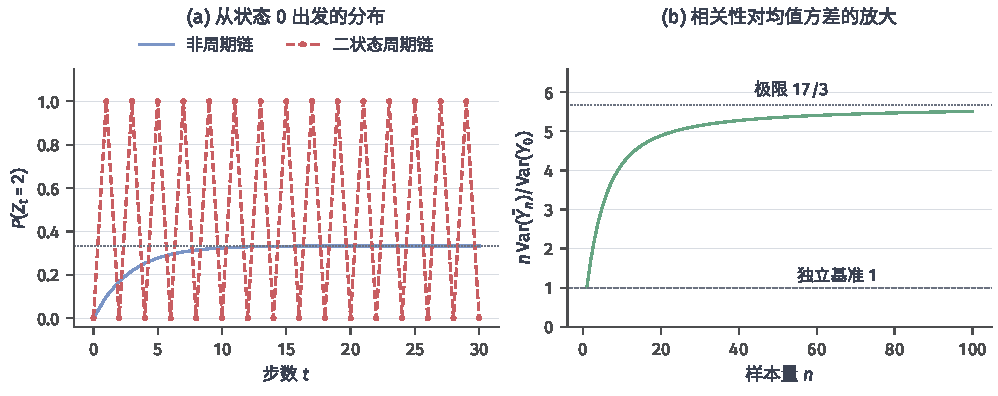
\includegraphics[width=\linewidth]{figures/01-mathematical-preliminaries/04-random-variables-distributions-and-causality/matplotlib/stochastic-mixing-variance/figure.pdf}
  \caption{两状态链的解析式教学图。左图蓝线使用例~\ref{ex:stoch-two-state-chain}的转移矩阵，从\(Z_0=0\)出发绘制\(\mathbb P(Z_t=2)=(1-0.7^t)/3\)；红线使用确定交替的转移矩阵。右图使用平稳初态和\(\rho_k=0.7^k\)，绘制\(1+2\sum_{k=1}^{n-1}(1-k/n)\rho_k\)，其极限为\(17/3\)，独立观测基准为\(1\)。}
  \label{fig:stochastic-mixing-variance}
\end{figure*}

\subsubsection{泊松过程}
\label{sec:rv-poisson}
事件到达使状态按次跳变。固定窗口内的计数可以服从Poisson分布，但只有规定不同窗口间的联合关系，才能得到Poisson过程。

\paragraph{事件计数与短时跳跃}
\begin{definition}[齐次Poisson过程]
\label{def:rv-poisson-process}
给定速率\(\lambda>0\)和滤过\((\mathcal F_t)_{t\geq0}\)，计数过程
\((N_t)_{t\geq0}\)称为相对于该滤过的齐次\term{泊松过程}（Poisson process），若它适应于滤过，
\(N_0=0\)几乎必然，路径几乎必然右连续、非减、取非负整数且每次跳跃为一，并满足
\[
N_t-N_s\ \perp\ \mathcal F_s,\qquad
N_t-N_s\sim\operatorname{Poisson}(\lambda(t-s)),
\quad 0\leq s<t.
\]
\end{definition}
这里的平稳性属于增量，而非\(N_t\)本身：计数均值随时间线性增长。
对互不相交、按时间排列的区间，逐步使用独立于过去的条件，便得到增量相互独立。
相对于自然滤过给出过程后，不能随意加入未来信息而仍称其增量独立于历史。

短区间\(h\downarrow0\)内，
\[
\begin{aligned}
\mathbb P(N_{t+h}-N_t=0)&=1-\lambda h+O(h^2),\\
\mathbb P(N_{t+h}-N_t=1)&=\lambda h+O(h^2),\\
\mathbb P(N_{t+h}-N_t\geq2)&=O(h^2).
\end{aligned}
\]
一次跳跃的\emph{概率}是一阶小量，发生跳跃时的\emph{幅度}却始终为一。
令\(T_k=\inf\{t:N_t\geq k\}\)为第\(k\)次到达时刻。有限\(t\)内
\(N_t<\infty\)几乎必然，因而只有有限次跳跃；这是有限活动过程。
左极限\(N_{t-}=\lim_{s\uparrow t}N_s\)记录跳跃发生前的计数，跳跃量记为
\(\Delta N_t=N_t-N_{t-}\)。

Poisson计数与指数等待是同一齐次到达机制的两个侧面。首次到达时间满足
\[
% Baseline P:914-923
  \mathbb{P}(T_1>t)
  =
  \mathbb{P}(N(t)=0)
  =
  e^{-\lambda t}.
\]
所以\(T_1\)服从速率为\(\lambda\)的指数分布；独立平稳增量进一步使相邻到达间隔独立
同分布。反过来，用独立同分布的指数等待时间累加生成到达时刻，所得计数过程的
\(N(t)\)服从\(\operatorname{Poisson}(\lambda t)\)。这里的联系依赖齐次性和独立增量，
不能由两个边缘分布的名称单独推出。
更具体地，独立增量的短区间概率给出前\(k\)个到达时刻在
\(0<t_1<\cdots<t_k\)上的联合密度
\(\lambda^k e^{-\lambda t_k}\)。换成等待间隔
\(E_i=T_i-T_{i-1}\)，其中\(T_0=0\)，Jacobian为一，密度变成
\(\prod_i\lambda e^{-\lambda e_i}\)，证明间隔独立且均为指数分布。
等待\(k\)次到达的总时长因此是
\(\operatorname{Gamma}(k,\lambda)\)，采用前面约定的速率参数。
反向从独立指数间隔构造时，
\(\mathbb P(T_k\leq t<T_{k+1})=e^{-\lambda t}(\lambda t)^k/k!\)；
无记忆性保证每个确定时刻之后的剩余等待仍指数，从而得到独立平稳增量。

若每次到达还带来随机量\(J_k\)，其中\(J_k\)独立同分布且独立于计数过程，则
\[
C_t=\sum_{k=1}^{N_t}J_k
\]
称为\term{复合泊松过程}（compound Poisson process）。其跳跃量不必为一，也可为负；给定\(N_t\)以后再求条件均值和全方差，可得
\[
\mathbb EC_t=\lambda t\,\mathbb EJ_1,\qquad
\operatorname{Var}(C_t)=\lambda t\,\mathbb EJ_1^2
\]
（第一式需一阶绝对矩有限，第二式需二阶矩有限）。第二式不是
\(\lambda t\operatorname{Var}(J_1)\)，因为事件数本身也随机。
这里的Poisson过程描述事件到达；定义~\ref{def:stoch-markov-poisson-equation}中的Poisson方程描述Markov核下的均值校正，它们不是同一个对象。

\paragraph{平均到达与补偿增量}
计数每段时间平均增加\(\lambda h\)。从原计数中减去这一可预测平均趋势，得到\term{补偿泊松过程}（compensated Poisson process）
\[
\widetilde N_t=N_t-\lambda t.
\]
\begin{theorem}[Poisson补偿的鞅性质]
\label{thm:rv-compensated-poisson}
相对于定义~\ref{def:rv-poisson-process}中的滤过，
\(\widetilde N_t\)是平方可积鞅，且
\[
\mathbb E[(\widetilde N_t-\widetilde N_s)^2\mid\mathcal F_s]
=\lambda(t-s),\qquad
\widetilde N_t^2-\lambda t\text{也是鞅}.
\]
\end{theorem}
\begin{proof}
独立增量使给定\(\mathcal F_s\)后的计数增量仍有均值及方差
\(\lambda(t-s)\)。减去均值后，条件均值为零，条件二阶矩就是该方差。
再展开
\(\widetilde N_t^2=(\widetilde N_s+
(\widetilde N_t-\widetilde N_s))^2\)，交叉项条件期望为零，剩余新增二阶矩为
\(\lambda(t-s)\)，得到最后一个鞅结论。
\end{proof}
补偿并未抹平跳跃。图~\ref{fig:rv-poisson-compensation}中，计数在到达之间保持不变，补偿路径则以斜率\(-\lambda\)下降；每个到达时刻仍向上跳一。
\begin{figure}[htbp]
  \centering
  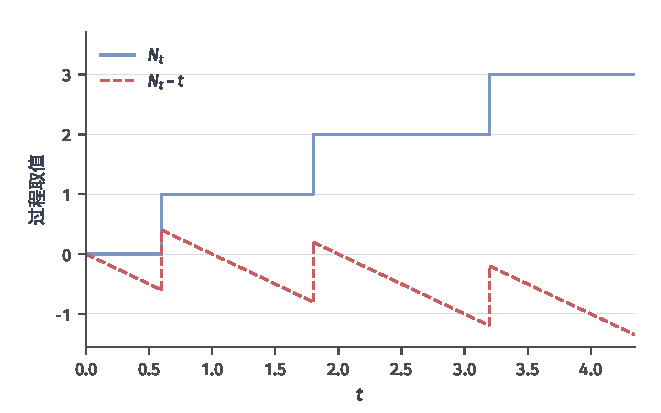
\includegraphics[width=\linewidth]{figures/01-mathematical-preliminaries/04-random-variables-distributions-and-causality/matplotlib/rv-poisson-compensation/figure.pdf}
  \caption{给定三次到达时刻的教学路径，取\(\lambda=1\)。蓝线为计数\(N_t\)，红虚线为\(\widetilde N_t=N_t-t\)；两条路径在同一时刻跳跃且跳跃量相同。减去的是平均趋势，不是实现中的跳跃。}
\label{fig:rv-poisson-compensation}
\end{figure}
平方跳跃累计为
\(\sum_{s\leq t}(\Delta\widetilde N_s)^2=N_t\)，是随机量；
其可预测平均累计为\(\lambda t\)，不是同一个量。在有限活动区间上，细分路径的平方增量和趋向跳跃平方和，连续线性漂移贡献趋零，故可记
\[
[\widetilde N]_t=N_t,\qquad
\langle\widetilde N\rangle_t=\lambda t.
\]
后一个量是使\(\widetilde N_t^2-\langle\widetilde N\rangle_t\)成为鞅的可预测补偿，呼应离散可预测二次变差。对确定分割，这个有限活动情形的路径计算可逐条进行；连续粗糙路径的二次变差将在下一例说明。

复合情形若\(\mathbb E|J_1|<\infty\)，则
\(C_t-\lambda t\,\mathbb EJ_1\)相对于只揭示已到达标记的自然历史是鞅。
若再有\(\mathbb EJ_1^2<\infty\)，其平方跳跃累计为
\(\sum_{k\leq N_t}J_k^2\)，可预测二阶累计为
\(\lambda t\,\mathbb EJ_1^2\)。例如每次损失恒为二，平均损失速率为\(2\lambda\)，二阶累计速率却为\(4\lambda\)。
随机积分将把在跳跃前确定的系数乘到这些补偿增量上；仅对有限步进系数而言，正交性已经给出
\[
\mathbb E\left(\sum_iH_i
(\widetilde N_{t_{i+1}}-\widetilde N_{t_i})\right)^2
=\lambda\sum_i\mathbb E H_i^2(t_{i+1}-t_i),
\quad H_i\in L^2(\mathcal F_{t_i}),
\]
这里使用确定分割与可预测系数。一般过程积分的定义及闭包条件见
第~\ref{chap:action-and-state}章“行动和状态”，其中
第~\ref{sec:action-state-poisson-integral}节将把这一有限和延拓为补偿Poisson积分。

\subsubsection{布朗运动}
\label{sec:dynamical-brownian-motion}
与一次一次的跳跃相对，连续波动的每段增量可越来越小，但累计波动仍然非零。布朗运动给出这种尺度的基本模型；连续路径不等于可微路径。

\paragraph{连续路径与增量尺度}
% Baseline D:1435-1490

设$\xi_{1},\xi_{2},\ldots$独立同分布， $\mathbb{E}\xi_{i}=0$、$\operatorname{Var}
(\xi_{i})=1$。 步长为$\Delta t$时，定义随机游走增量
\[
	\Delta X_{k}=\sqrt{\Delta t}\,\xi_{k}.
\]
经过$n=t/\Delta t$步，
\[
	\operatorname{Var}\left( \sum_{k=1}^{n}\Delta X_{k}\right) = n\Delta t=t.
\]
若把增量缩放成$\Delta t\,\xi_{k}$， 方差会随$\Delta t\to0$趋零；
若不缩放，固定时间内方差会发散。
平方根尺度是让连续时间极限保留有限非零波动的尺度。

在有限方差及适当插值条件下， 函数型中心极限定理把缩放随机游走连接到\term{布朗运动}（Brownian motion）。 本章不重证该一般弱收敛定理，
而从极限所需的性质定义连续对象。

\begin{definition}[标准布朗运动]
	\label{def:dynamical-standard-brownian-motion} 实值过程$(W_{t})_{t\geq0}$称为标准布朗运动，
	若它满足：
	\begin{enumerate}
		\item $W_{0}=0$几乎必然成立；

		\item 对$0\leq t_{0}<t_{1}<\cdots<t_{n}$， 增量$W_{t_i}-W_{t_{i-1}}$相互独立；

		\item $W_{t}-W_{s}\sim\mathcal{N}(0,t-s)$，其中$0\leq s<t$；

		\item 样本路径几乎必然连续。
	\end{enumerate}
\end{definition}

当布朗运动与滤过$(\mathcal{F}_t)_{t\geq0}$共同使用时，还要求$W_t$对该滤过适应，
并且对$s<t$，增量$W_t-W_s$独立于$\mathcal{F}_s$。
定义中的独立增量只比较布朗运动自身的不同时间段；加入滤过后的条件保证积分中的“过去信息”
不能预见下一段布朗增量。

由独立增量和方差公式，
\begin{equation}
	\mathbb{E}[W_{s}W_{t}]=\min(s,t). \label{eq:dynamical-brownian-covariance}
\end{equation}
例如$s\leq t$时， $W_{t}=W_{s}+(W_{t}-W_{s})$， 后一增量与$W_{s}$独立且均值为零，
所以协方差为$\mathbb{E}W_{s}^{2}=s$。

\par\medskip\noindent\textbf{布朗运动的尺度与路径正则性}\quad
对任意$c>0$，过程
\[
	\widetilde W_{t}= c^{-1/2}W_{ct}
\]
仍是标准布朗运动。 它从零出发，增量仍独立， 并且
\[
	\widetilde W_{t}-\widetilde W_{s}\sim \mathcal{N}(0,t-s).
\]
连续性也由原路径继承。 因此两过程具有相同的有限维分布。
这就是布朗运动的尺度规律。

相对于同一滤过，\(m\)维标准Brownian运动
\(\bm W_t=(W_t^{(1)},\ldots,W_t^{(m)})^\top\)由相互独立的实值标准Brownian运动组成，并要求
\[
\bm W_t-\bm W_s\ \perp\ \mathcal F_s,\qquad
\bm W_t-\bm W_s\sim\mathcal N(\bm0,(t-s)\bm I_m).
\]
若以固定矩阵\(\bm A\)混合这些分量，增量协方差变成
\((t-s)\bm A\bm A^\top\)，不再是标准Brownian的单位协方差；低秩\(\bm A\)允许退化扩散。

\paragraph{不可微性与二次变差}
% Baseline D:1492-1542
长度为\(h\)的增量典型尺度为\(\sqrt h\)，所以差商
\[
	\frac{W_{t+h}-W_{t}}{h}
\]
的标准差为$1/\sqrt{h}$， 随$h\to0$反而发散。 严格结果表明，以概率$1$，
布朗运动的样本路径在所有时刻连续，同时在任何时刻都不可微。
因此不能把$\mathrm{d}W_{t}/\mathrm{d}t$当作普通随机函数， 再用Riemann积分处理。

\par\medskip\noindent\textbf{布朗运动的二次变差}\quad
二次变差记录细分以后仍无法消失的平方波动。它与$\operatorname{Var}(W_t)$不同：
方差在固定时刻跨样本求平均，二次变差沿同一条路径对时间增量求和再取极限。
取$[0,t]$的一列确定分割$0=t_0<\cdots<t_n=t$，其最大区间长度趋零，并记平方增量和
\[
	Q_{n}= \sum_{i=0}^{n-1}(W_{t_{i+1}}-W_{t_i})^{2}.
\]
\begin{definition}[沿确定分割的二次变差]
\label{def:dynamical-quadratic-variation}
若连续过程沿每一列网格趋零的确定分割得到的平方增量和，在时刻$t$都依概率收敛到同一个随机变量，
这个极限记为$[X]_t$，称为该过程在$[0,t]$上的二次变差。
\end{definition}
以下计算证明标准布朗运动的极限为确定量$t$，并且收敛甚至在$L^2$中成立。
其期望为
\[
	\mathbb{E}Q_{n}= \sum_{i}(t_{i+1}-t_{i})=t.
\]
独立高斯增量还给出
\[
	\operatorname{Var}(Q_{n}) = 2\sum_{i}(t_{i+1}-t_{i})^{2}\leq 2t\max_{i}(t_{i+1}
	-t_{i}).
\]
因此网格趋零时， $Q_{n}\to t$在$L^{2}$中成立，进而依概率成立。 这称为布朗运动在$[
0,t]$上的二次变差等于$t$。

普通连续可微路径的平方增量和会趋零， 因为每个增量是$O(\Delta t)$， 平方后求和为$O
(\Delta t)$。 布朗增量是$O_{\mathbb{P}}(\sqrt{\Delta t})$， 平方后恰好是$O_{\mathbb{P}}
(\Delta t)$。 后文的Itô公式之所以保留二阶导数项， 根源就在这个非零二次变差。

图~\ref{fig:reader-brownian-quadratic-variation}用同一组细网格高斯增量形成两种分割。
平方和随分割改变，但细分后趋近的是$t$，而不是左图路径在时刻$t$的高低。
单条教学折线只能说明计算对象，依概率收敛的保证来自刚才对任意确定分割给出的方差上界。
\begin{figure*}[htbp]
  \centering
  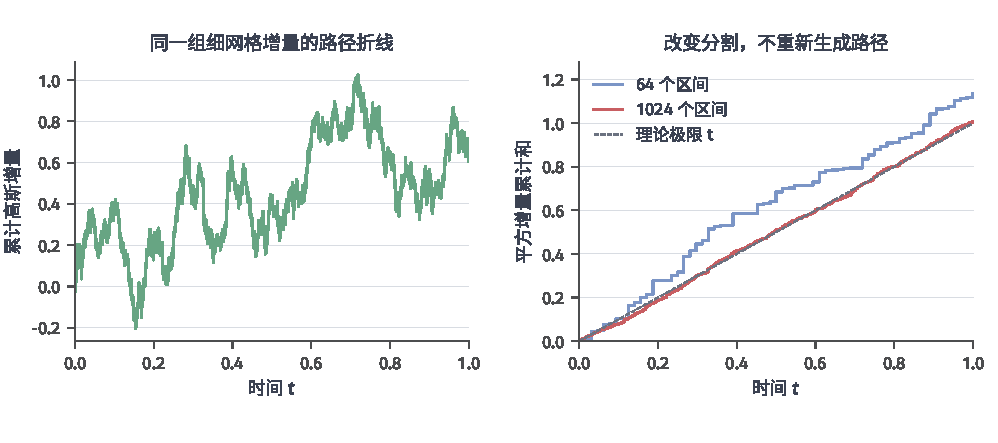
\includegraphics[width=\linewidth]{figures/01-mathematical-preliminaries/04-random-variables-distributions-and-causality/matplotlib/reader-brownian-quadratic-variation/figure.pdf}
  \caption{以固定随机种子构造的高斯增量教学例。左图由$4096$个独立增量
  $\Delta W_i\sim\mathcal N(0,1/4096)$累计成路径折线；右图将同一组增量分别合并为
  $64$和$1024$个时间区间，再累计各区间增量的平方。蓝、红阶梯线使用不同分割，
  灰色参考线为理论二次变差$t$。这里只绘制有限网格，不把某一条折线作为连续布朗路径或收敛证明。}
  \label{fig:reader-brownian-quadratic-variation}
\end{figure*}

平方增量会留下有限累计量，这使普通积分的链式法则不再适用。第~\ref{chap:dynamical-systems-and-state-estimation}章将用它建立随机积分与Itô换元。
差商在固定时刻的方差发散，是不可微的尺度提示，不是“几乎必然所有时刻都不可微”的完整证明；后者同时涉及不可数多个时刻，是严格路径定理。相应地，
\(W_{t+h}-W_t=O_{\mathbb P}(\sqrt h)\)不是对全部实现、全部短区间成立的统一确定性上界。

对同一确定分割，交叉二次变差使用增量乘积而非平方：
\[
[X,Y]_t=\lim_{|\pi|\to0}\sum_{[u,v]\in\pi}
(X_v-X_u)(Y_v-Y_u),
\]
这里按存在时的依概率极限理解。独立Brownian分量\(i\ne j\)的和均值为零，方差为
\(\sum_{[u,v]\in\pi}(v-u)^2\leq t|\pi|\)，所以
\([W^{(i)},W^{(j)}]_t=0\)；同一分量的计算则给出\(t\)。合写为
\([W^{(i)},W^{(j)}]_t=\delta_{ij}t\)。
在二进分割上，平方和方差界可求和，Borel--Cantelli还给出逐个固定终点的几乎必然收敛；对一般网格列，这里的无条件结论是已证明的\(L^2\)及依概率收敛，不把它加强成对所有分割同时逐路径成立。

\subsubsection{高斯过程}
% Baseline S:41-58
\begin{definition}[高斯过程]
  \label{def:stoch-gaussian-process}
  实值随机过程\((F(x))_{x\in\mathcal X}\)称为\term{高斯过程}（Gaussian process），若任意正整数\(m\)及任意\(x_1,\ldots,x_m\in\mathcal X\)上的向量
  \((F(x_1),\ldots,F(x_m))^\top\)均服从多元高斯分布，允许协方差奇异。其均值函数和协方差函数为
  \[
    m(x)=\mathbb E F(x),\qquad
    k(x,x')=\operatorname{Cov}(F(x),F(x')),
  \]
  因而每个有限向量的均值为\((m(x_i))_i\)，协方差矩阵为\((k(x_i,x_j))_{i,j}\)，记作\(F\sim\mathcal{GP}(m,k)\)。索引\(x\)不必代表时间。
\end{definition}
协方差函数必须对称，且对任意有限输入和实系数\(c_i\)满足
\[
  \sum_{i,j}c_ic_jk(x_i,x_j)\geq0.
\]
这正是有限协方差矩阵半正定的条件。均值与协方差因此确定高斯过程的全部有限维分布；它们本身不自动保证样本函数连续、可微或具有Markov性。

例如令\(A,B\)是独立标准高斯变量，定义\(F(x)=A+Bx\)。任意有限函数值都是\((A,B)\)的线性变换，所以构成高斯过程，且
\(m(x)=0\)、\(k(x,x')=1+xx'\)。三个以上不同输入的协方差矩阵可以奇异，因为这些随机值都由同两个随机系数决定。反过来，各点边缘高斯并不足够：若\(X\sim\mathcal N(0,1)\)，独立符号\(S\)等概率取\(\pm1\)，则\(X,SX\)的边缘均为标准高斯且不相关，但\((SX)^2=X^2\)使它们依赖，故不可能是联合高斯。定义中的“任意有限联合分布”不可省略。
布朗运动是均值零、核\(k(s,t)=\min(s,t)\)的高斯过程：每个有限向量都由独立高斯增量线性组合得到。这个核确实半正定，因为
\[
\sum_{i,j}c_ic_j\min(t_i,t_j)
=\int_0^\infty\left(\sum_i c_i\mathbb I_{\{u\leq t_i\}}\right)^2\,\mathrm du\geq0.
\]
一般给定均值和对称半正定核时，相应高斯有限维分布相容，可用第~\ref{sec:rv-finite-dimensional-laws}节的扩张定理建立过程。要得到连续版本，仍须对核控制增量矩；“高斯过程”这个名称本身不承诺路径光滑。

\section{随机变量的推断}
\label{sec:rv-inference}
此前给定概率规律，计算变量怎样变化；现在只有有限数据，规律本身未知。
\term{数理统计}（mathematical statistics）研究怎样从这些观测推断规律并量化误差。
估计要回答参数、分位数或分布是什么，预测要回答尚未观测的结果可能是什么。
样本不能唯一重建基础空间上的映射，推断只针对明确的分布及其目标。

先固定比较标准。行动\(a\)是报告的结论，损失\(\ell(a,\tau(\theta))\)衡量它偏离目标的代价，风险再对重复抽样取期望。估计量是抽样前的随机函数，估计值是观测后的具体数值。
% Baseline T:460-469
\begin{definition}[估计量的风险]
  \label{def:statistics-estimator-risk}
给定模型、目标泛函\(\tau\)和非负可测损失\(\ell\)，估计量的\term{风险}（risk）是
\[
  R_\theta(\widehat\tau)
  =\mathbb{E}_\theta[
    \ell(\widehat\tau(\bm Y),\tau(\theta))].
\]
它允许取\(+\infty\)，并随未知参数\(\theta\)变化。
\end{definition}

\subsection{观测制度与可识别目标}
\label{sec:stats-targets-data-sources}
误差计算之前，要分别核对目标能否被观测分布确定，以及样本究竟如何进入数据集。模型不可识别与有限样本不够精确是不同困难。

\subsubsection{推断目标与可识别性}
\label{sec:statistics-model-target}
% Baseline T:33-120
\begin{definition}[统计模型与统计量]
  \label{def:statistics-model-statistic}
\term{统计模型}（statistical model）是一族候选分布
\[
  \mathcal{P}=\{P_\vartheta:\vartheta\in\Theta\}.
\]
这些分布定义在同一个可测观测空间上，参数\(\vartheta\)是描述候选分布的未知索引。观测
\(\bm{Y}=(Y_1,\ldots,Y_n)\)由其中某个分布产生，但真实索引不可见。参数未必是
一个物理常数；它也可以是一组回归系数、一个混合比例，或者无限维的分布函数。

\term{统计量}（statistic）是只依赖样本的可测函数
\(T(\bm{Y})\)。当统计量被设计来逼近某个未知目标
\(\tau(\vartheta)\)时，它称为\term{估计量}（estimator），通常记为
\(\widehat{\tau}\)。在一批已经观测的数据\(\bm{y}\)上算出的
\(\widehat{\tau}(\bm{y})\)是\term{估计值}（estimate）。参数属于模型，估计量
在重复抽样中是随机变量，估计值则是一次计算得到的数；混淆三者会使“偏差”和
“不确定性”失去对象。
\end{definition}

推断目标可以有不同层次。估计\(\theta\)是在参数空间中找一个点；估计分布函数
\(F(y)\)是在函数空间中恢复整体规律；预测未来观测\(Y_{n+1}\)则还要保留新噪声。
即使都输出一个数，它们回答的也不是同一个问题。例如
\(\overline{Y}\)可估计位置\(\theta\)，而预测下一次读数还需要噪声尺度。
一般地，目标写成映射\(\tau:\Theta\to\mathcal A\)，其中
\(\mathcal A\)可以是标量、向量、函数或概率分布。能够只由可观察分布决定的目标也可
进一步写成分布泛函。估计误差还必须配合损失
\(\ell:\mathcal A\times\mathcal A\to[0,\infty]\)解释；向量目标的坐标平方误差、
总平方误差和某个方向上的误差是不同口径，不能只写“估计准确”。

在有限方差位置模型\(Y_i=\theta+\varepsilon_i\)中，若误差独立、均值为零且方差为
\(\sigma^2\)，则
\[
  \mathbb{E}_\theta[\overline Y]
  =\theta+\frac1n\sum_{i=1}^n\mathbb{E}[\varepsilon_i]
  =\theta,\qquad
  \operatorname{Var}_\theta(\overline Y)
  =\frac1{n^2}\sum_{i=1}^n\operatorname{Var}(\varepsilon_i)
  =\frac{\sigma^2}{n}.
\]
无偏性来自零均值，\(1/n\)方差缩减还使用了独立性；若误差相关，方差中必须保留
协方差项。

\par\medskip\noindent\textbf{识别、等价模型与推断边界}\quad
数据充足之前还要问目标能否由观测区分。
\begin{definition}[目标可识别性]
  \label{def:statistics-identifiability}
  给定统计模型\(\{P_\vartheta:\vartheta\in\Theta\}\)和目标泛函\(\tau:\Theta\to\mathcal T\)，若对所有\(\vartheta_1,\vartheta_2\in\Theta\)有
\[
  P_{\vartheta_1}=P_{\vartheta_2}
  \quad\Longrightarrow\quad
  \tau(\vartheta_1)=\tau(\vartheta_2),
\]
就称目标\(\tau\)在模型中是\term{可识别的}（identifiable）。
\end{definition}
取
\(\tau(\vartheta)=\vartheta\)时，这一定义才退化为参数可识别。可识别性是总体分布
层面的性质，不是有限样本算法的表现。

\begin{example}[混合成分的标签交换]
\label{ex:statistics-mixture-label-switching}
设观测来自二成分高斯混合
\[
  p(y)=\pi\phi(y;\mu_1,\sigma^2)
       +(1-\pi)\phi(y;\mu_2,\sigma^2).
\]
把\((\pi,\mu_1,\mu_2)\)换成
\((1-\pi,\mu_2,\mu_1)\)不改变分布。若“第一成分”只表示编号，参数便有两种等价
表示；添加\(\mu_1<\mu_2\)之类约束可以固定表示，却没有创造新的观测信息。
\end{example}

另一种失败来自来源一起出错。若所有温度计都有未知共同偏移\(b\)，模型为
\(Y_i=\theta+b+\varepsilon_i\)，观测只识别\(\theta+b\)，不能分别识别
\(\theta\)和\(b\)。增加同型号温度计会减小随机噪声，却不会消除共同偏差。由此可见，
“有很多数据”“目标可识别”和“目标容易准确估计”是三项不同判断。

不可识别还直接限制任何估计程序。若
\(P_{\vartheta_1}=P_{\vartheta_2}\)但
\(\tau(\vartheta_1)\neq\tau(\vartheta_2)\)，取两目标值距离的三分之一为
\(\epsilon>0\)。任何只依赖样本的估计量\(\widehat\tau_n\)在两种机制下具有相同
分布，因而不可能同时满足
\[
  \mathbb{P}_{\vartheta_j}
  \left\{\lVert\widehat\tau_n-\tau(\vartheta_j)\rVert<\epsilon\right\}
  \longrightarrow1,\qquad j=1,2.
\]
因为两个半径为\(\epsilon\)的球不相交，同一个估计量分布不可能把趋近于一的概率
同时赋给它们。这证明了：不可识别目标不能靠增加同类样本在全部等价机制下一致恢复。

\subsubsection{抽样方式与观测机制}
\label{sec:statistics-sampling-population}
\label{sec:statistics-missingness-observation}
% Baseline T:127-251
统计结论必须先回答“想对谁成立”。\term{目标总体}（target population）是推断希望
覆盖的对象、时间和条件的集合；\term{抽样制度}（sampling regime）描述观测如何从
这些对象产生。若样本只来自工作日的一个传感器，模型本身不能把结论自动推广到周末或
另一批设备。

独立同分布抽样把每个\(Y_i\)视为来自同一分布的独立重复。配对抽样则把
\((Y_{i,A},Y_{i,B})\)视为一个单位，例如同一对象在两种条件下的读数。此时差值
\(D_i=Y_{i,A}-Y_{i,B}\)才是独立单位；把两列拆成\(2n\)个独立记录会丢失配对信息。
分层抽样预先按群组分别抽取，成组抽样则一次抽取整个设备、班级或用户群。两者的
独立单位和加权方式不同。

\par\medskip\noindent\textbf{条件分母、相关性与信息量}\quad
配对的收益取决于对内协方差：
\[
  \operatorname{Var}(D_i)
  =\operatorname{Var}(Y_{i,A})+\operatorname{Var}(Y_{i,B})
   -2\operatorname{Cov}(Y_{i,A},Y_{i,B}).
\]
正协方差会降低差值方差，负协方差则可能使配对更差；“同一对象测两次”本身并不保证
精度提高。

设目标总体中群组\(g\)的比例为\(\pi_g\)，群组均值为\(\mu_g\)，则总体均值为
\[
  \mu=\sum_g\pi_g\mu_g.
\]
总体指标可能很好，却掩盖某个小群组的严重误差。若群组中有\(n_g\)个独立Bernoulli
结果，样本比率\(\widehat p_g\)的方差为
\[
  \operatorname{Var}(\widehat p_g)
  =\frac{p_g(1-p_g)}{n_g}.
\]
这里把\(n_g\)视为固定正整数。若群组样本数
\(N_g=\sum_i\mathbb{I}\{G_i=g\}\)也是随机的，则
\(\widehat p_g\)只在\(N_g>0\)时有定义，且上述方差是给定\(N_g\)后的条件方差；
无条件误差还要平均随机分母，并处理\(N_g=0\)事件。不确定性由实际相关分母决定，
而不是总样本量\(n\)。报告群组公平性或来源质量时，应同时报告分母、抽样方式和区间，
不能只排列百分比。

已知入样概率时，权重可以把抽样分布重新接回目标总体。令\(S\in\{0,1\}\)表示一个
总体对象是否入样，\(\rho(Z)=\mathbb{P}(S=1\mid Z)\)，并假设
\(S\mathrel{\perp}Y\mid Z\)、\(\rho(Z)>0\)以及
\(\mathbb{E}[|Y|/\rho(Z)]<\infty\)。条件期望给出
\[
  \mathbb{E}\left[\frac{SY}{\rho(Z)}\right]
  =\mathbb{E}\left[
    \frac{\mathbb{E}[S\mid Y,Z]Y}{\rho(Z)}
  \right]
  =\mathbb{E}[Y].
\]
这条逆概率恒等式恢复的是明确的总体平均。若某一区域\(\rho(Z)=0\)，或者入样在给定
\(Z\)后仍依赖未观测的\(Y\)，等式便不能由现有数据推出。

记录数也不等于独立信息量。若同一来源复制一条记录十次，样本平均的显示分母增大，
实际信息却没有增加。时间序列中的相邻读数可能共享漂移；群组内记录可能共享设备偏差。
这类依赖应通过按群组建模、块抽样或
第~\ref{sec:stoch-markov-long-run-average}节的相关过程工具处理，而不能
继续套用独立样本方差。

时间抽样还会改变目标本身。若传感器每分钟记录一次，而目标是“一天中随机时刻的平均
读数”，等间隔采样与目标一致；若只在告警后加密采样，朴素平均就会过度代表异常时段。
一种修正方式是记录每个时段被抽中的概率并作逆概率加权，但这要求所有目标时段都有正的
入样概率。完全未覆盖的夜间时段不能靠增大已有权重恢复。抽样日志因此也是统计数据的一
部分。

抽样制度与分析单位应在看结果前确定。假设十台设备各产生一千条记录，而处理实际随机
分配给设备，那么有效随机化单位是十台设备，不是一万条记录。记录内噪声可以帮助估计
每台设备的均值，却不能把处理效应的独立单位扩充到一万。这个区别会同时影响标准误、
置换方式和训练测试划分。

\par\medskip\noindent\textbf{缺失、选择与可忽略性}\quad

不完整观测带来另一类问题。令\(R=1\)表示\(Y\)被观察到，\(X\)为始终可见变量。
\term{完全随机缺失}（missing completely at random, MCAR）要求
\[
  R\mathrel{\perp}(X,Y).
\]
\term{随机缺失}（missing at random, MAR）要求
\[
  R\mathrel{\perp}Y\mid X,
\]
即给定已观测协变量后，缺失概率不再依赖缺失值本身。
\term{非随机缺失}（missing not at random, MNAR）则允许这种剩余依赖。

多个变量可能按不同模式缺失，此时“已观测变量”随模式改变，不能用一个固定条件集概括全部MAR要求。
\begin{definition}[观测模式与缺失机制]
  \label{def:statistics-missingness}
  设完整数据为\(\bm Z=(Z_1,\ldots,Z_d)\)，观测指示\(\bm R\in\{0,1\}^d\)。对每种模式\(\bm r\)，定义
  \[
    O(\bm r)=\{j:r_j=1\},\qquad M(\bm r)=\{j:r_j=0\}.
  \]
  实际记录为\((\bm r,\bm Z_{O(\bm r)})\)。令\(g(\bm r\mid\bm z)\)为给定完整数据时的模式概率核。若对每种\(\bm r\)都存在只依赖已见坐标的可测函数\(g_{\bm r}\)，使
  \[
    g(\bm r\mid\bm z)=g_{\bm r}(\bm z_{O(\bm r)})
  \]
  对完整数据分布几乎处处成立，则称机制为MAR。若\(g(\bm r\mid\bm z)\)对全部模式均不依赖\(\bm z\)，则为MCAR；若MAR条件失败，则为MNAR。
\end{definition}
例如在二维数据中，模式\((1,0)\)的出现概率可依赖\(Z_1\)，却不能依赖未见的\(Z_2\)；模式\((0,1)\)反过来可以依赖\(Z_2\)，却不能依赖\(Z_1\)。这是对每种模式分别施加的条件，不能只在当前观测到的某一模式上核对。“随机缺失”也不等于“缺失标记完全随机”，后者对应更强的MCAR。

当\(\mathbb{P}(R=1)>0\)时，MCAR下完整案例仍代表总体，但效率降低。MAR下可建模
\(\mathbb{P}(R=1\mid X)\)并加权，或建模\(Y\mid X\)后插补；两者都依赖模型和
正值条件。MNAR通常不能只靠已观测数据识别，需要机制假设、外部信息或敏感性分析。
MAR描述的是缺失概率依赖哪些变量，并不意味着可以丢弃所有不完整记录。
“缺失机制可忽略”则要指定在哪一种推断计算中省去机制项；定义似然后，
式~\eqref{eq:statistics-missing-likelihood}将说明这种省略还需要哪些参数条件。
数据表中的一个缺失标记本身不能证明属于哪种机制。

识别障碍在有界结果上已经出现。若\(0\leq Y\leq1\)且
\(\mathbb{P}(R=0)>0\)，观测数据只给出已见部分的\(RY\)与缺失指示；把所有未见
\(Y\)设为\(0\)或设为\(1\)会产生相同观测，却给出不同总体均值。因此不加机制条件
时只能得到
\[
  \mathbb{E}[RY]
  \leq\mathbb{E}[Y]
  \leq\mathbb{E}[RY]+\mathbb{P}(R=0).
\]
两个端点分别可由把全部未见结果设为\(0\)或\(1\)达到，所以仅凭上述信息不能继续
收紧。若MAR成立，并令
\(\pi(X)=\mathbb{P}(R=1\mid X)>0\)，则第
~\ref{sec:statistics-sampling-population}节的逆概率恒等式在这里化为
\[
  \mathbb{E}\left[\frac{RY}{\pi(X)}\right]
  =\mathbb{E}[Y].
\]
正值条件负责覆盖，条件独立负责把未见结果接回已见结果；权重很大时，即使目标可识别，
有限样本方差仍可能很高。
\begin{example}[贯穿本章的传感器校准数据]
\label{ex:statistics-running-sensor-calibration}
考虑教学构造的\(25\)个独立传感器响应，暂以高斯位置模型描述，单次噪声标准差已知为
\(\sigma=2\)，样本汇总为
\[
\overline y=10.4,\qquad
\frac1{25}\sum_{i=1}^{25}(y_i-\overline y)^2=4.
\]
若另问响应如何随校准输入\(x\)变化，靠近左边界\(x_0=0\)的三个观测为
\[
(x_i,y_i)=(0,9),(1,11),(3,13),
\]
在给定带宽下核权重为\(1,0.75,0.25\)。后面的局部回归、Bootstrap、区间与预测复用这些输入，只改变所报告的目标。它们是可核算的教学数值，不是实测性能报告；把局部输入关系加入模型时，也不再把全部读数视为同一位置分布的重复抽取。
\end{example}

\subsection{分布与分布特征的估计}
\label{sec:stats-parameter-inference-efficiency}
报告一个均值和报告整张分布是不同输出，但不等于参数方法与非参数方法的划分。经验均值可以不预设参数族，整张高斯分布也可以由有限参数估计；似然、矩、损失和先验则是这些任务中可组合使用的构造依据。

\subsubsection{有限维目标的估计}
\label{sec:statistics-likelihood-robustness}
\label{sec:statistics-bayes-hierarchy}
% Baseline T:266-439
给定观测\(\bm{y}\)后，\term{似然}（likelihood）
\[
  L(\vartheta;\bm{y})=p_\vartheta(\bm{y})
\]
相对于模型共同的参考测度定义，把数据固定，把参数看作待比较的变量。似然不是参数的
概率分布；只有再指定先验并归一化后，才得到后验分布。最大似然估计选择
\(\widehat\vartheta_{\mathrm{MLE}}\in\argmax_\vartheta L(\vartheta;\bm{y})\)，
通常等价于最小化负对数似然\scite{vanderVaart1998asymptotic}

现在可以明确前面的缺失机制可忽略性。以连续数据为例，令\(p_\theta\)描述完整数据，
\(g_\psi\)描述缺失模式；\(\theta\)与\(\psi\)分别是两者的参数。若整个模型满足MAR，
固定已见模式\(\bm r\)与坐标\(\bm z_{\mathrm{obs}}\)后，观测似然分解为
\begin{equation}
\begin{aligned}
 L_{\mathrm{obs}}(\theta,\psi)
 &=\int p_\theta(\bm z_{\mathrm{obs}},\bm z_{\mathrm{mis}})
       g_\psi(\bm r\mid\bm z_{\mathrm{obs}})\,\mathrm d\bm z_{\mathrm{mis}}\\
 &=g_\psi(\bm r\mid\bm z_{\mathrm{obs}})
       L_{\mathrm{data}}(\theta),\\
 L_{\mathrm{data}}(\theta)
 &=\int p_\theta(\bm z_{\mathrm{obs}},\bm z_{\mathrm{mis}})
       \,\mathrm d\bm z_{\mathrm{mis}}.
\end{aligned}
\label{eq:statistics-missing-likelihood}
\end{equation}
离散坐标把相应积分换成求和。若参数域是直积\(\Theta\times\Psi\)，即两组参数可独立变化，
在机制因子为正的观测上比较\(\theta\)的似然时便可省去这个不含\(\theta\)的因子。
这里省去的是机制模型的计算，保留的是对缺失坐标积分后的数据似然；直接删除不完整行
不是这项分解允许的操作。

对\(Y_i\overset{\mathrm{iid}}{\sim}\mathcal{N}(\theta,\sigma^2)\)，且
\(\sigma^2\)已知，
\[
  -\log L(\theta;\bm{y})
  =\frac{1}{2\sigma^2}\sum_{i=1}^n(y_i-\theta)^2+C.
\]
对\(\theta\)求导并令其为零，得到
\(\widehat\theta=\overline y\)。同一个样本平均也可由矩估计得到：总体矩
\(\mathbb{E}_\theta[Y]=\theta\)，于是令样本矩\(\overline Y\)等于总体矩。
似然法依赖完整分布形式，矩估计只使用选定矩条件。

“令导数为零”只寻找内点候选，不保证最大值存在或唯一。例如独立Bernoulli观测的
似然为
\[
  L(p;\bm y)=p^{\sum_i y_i}(1-p)^{n-\sum_i y_i},\qquad p\in[0,1].
\]
当样本同时含有\(0\)和\(1\)时，唯一最大值是样本比例；全为\(1\)或全为\(0\)时，
最大值分别落在边界\(p=1\)或\(p=0\)。若错误地把参数域写成开区间\((0,1)\)，
边界数据甚至只有上确界而没有最大似然估计。

压缩数据会丢掉细节，但有时这些细节与目标参数无关。例如Bernoulli样本的排列不同，只要成功次数相同，似然关于\(p\)的依赖就相同。充分性要求这种“保留全部参数信息”在整个指定模型中成立。
\begin{definition}[充分统计量]
  \label{def:statistics-sufficient-statistic}
  设样本\(\bm Y\)与统计量\(T(\bm Y)\)取值于标准Borel空间。若存在概率核\(K(t,\cdot)\)，对每个\(\vartheta\in\Theta\)都是\(\bm Y\)给定\(T=t\)的正则条件分布版本，而且\(K\)不依赖\(\vartheta\)，则称\(T\)为该模型的\term{充分统计量}（sufficient statistic）。各条件分布的等式按相应\(P_\vartheta^T\)-几乎处处意义理解。
\end{definition}
它是在给定摘要后，样本其余部分不再携带关于参数的信息。在受同一个\(\sigma\)有限测度支配的模型中，若密度可分解为
\[
  p_\vartheta(\bm y)=g_\vartheta(T(\bm y))h(\bm y),
\]
则因子分解定理说明\(T\)对\(\vartheta\)充分。直观地说，给定
\(T(\bm Y)=t\)后，条件密度中的参数因子在归一化时抵消，剩余分布不含
\(\vartheta\)。在有限离散样本空间上，逆向关系也可直接算出。若
\(\bm Y\mid T=t\)的条件质量\(k(\bm y\mid t)\)不依赖参数，则
\[
  p_\vartheta(\bm y)
  =p_\vartheta^T(T(\bm y))k(\bm y\mid T(\bm y)),
\]
也得到所需分解。一般连续情形的条件分布可能集中在低维纤维上，不能把这个离散乘法式未经参考测度核对就当成普通密度恒等式；因子分解定理负责一般受支配模型中的等价性。高斯位置模型中，已知方差时
\(\sum_iY_i\)充分。充分性是相对于指定模型而言的；模型失配后，压缩掉的部分可能正好
暴露失配。

\par\medskip\noindent\textbf{M估计、矩估计与伪真目标}\quad
似然以指定模型的对数密度作为拟合准则。若目标是中位数、希望减轻异常值影响，或不愿假定完整分布形状，就需要按目标另选样本准则。下面的表达把这些估计方法放在同一个框架中，但不同准则的总体最小点未必相同。
\begin{definition}[M估计]
  \label{def:statistics-m-estimator}
给定可测准则\(\rho(y,\vartheta)\)，当下面的最小点集合非空且存在可测选择时，\term{\(M\)估计}（M-estimation）是从中选出的一个可测统计量：
\[
  \widehat\vartheta
  \in\argmin_{\vartheta\in\Theta}
  \frac1n\sum_{i=1}^n\rho(Y_i,\vartheta).
\]
\end{definition}
可微时，一阶条件是估计方程
\[
  \frac1n\sum_{i=1}^n\psi(Y_i,\widehat\vartheta)=0,
  \qquad
  \psi(y,\vartheta)=\nabla_\vartheta\rho(y,\vartheta).
\]
平方损失给出\(\psi(y,\theta)=\theta-y\)，每个残差的作用随绝对值线性增长。
若\(\mathbb E|Y|<\infty\)，绝对损失\(\rho(y,\theta)=|y-\theta|\)的总体风险有限，
其最小点则是中位数：目标函数的左右
方向导数分别由\(\mathbb{P}(Y<\theta)\)与\(\mathbb{P}(Y>\theta)\)决定，最优条件是
\(\mathbb{P}(Y\leq\theta)\geq1/2\)且
\(\mathbb{P}(Y\geq\theta)\geq1/2\)。因此平方与绝对准则即使使用同一批位置数据，
也在估计不同的总体泛函。

\(M\)估计的一致性需要把经验准则与总体准则连接起来。记
\[
  Q_n(\vartheta)=\frac1n\sum_{i=1}^n\rho(Y_i,\vartheta),
  \qquad
  Q(\vartheta)=\mathbb{E}[\rho(Y,\vartheta)].
\]
假设\(\Theta\)紧，\(Q\)在唯一点\(\vartheta^\star\)取得最小值，并且该最小值
分离，即对每个\(\epsilon>0\)，
\[
  \inf_{\lVert\vartheta-\vartheta^\star\rVert\geq\epsilon}
  Q(\vartheta)>Q(\vartheta^\star).
\]
若\(\sup_{\vartheta\in\Theta}|Q_n(\vartheta)-Q(\vartheta)|
\xrightarrow{\mathbb{P}}0\)，且近似优化误差
\[
  Q_n(\widehat\vartheta_n)-\inf_{\vartheta\in\Theta}Q_n(\vartheta)
  =o_{\mathbb{P}}(1),
\]
其中\(o_{\mathbb{P}}(1)\)表示该随机误差依概率趋于零，则
\(\widehat\vartheta_n\xrightarrow{\mathbb{P}}\vartheta^\star\)。证明只需比较准则：
在任意固定的\(\epsilon\)球外，总体准则有正间隔；当一致偏差和优化误差都小于该
间隔的适当分数时，经验近似最小点不可能位于球外。若参数空间不紧，则必须另证估计点
不会逃向无穷远；若总体最小点不唯一，结论只能指向最小点集合。

若真实分布\(Q\)不属于\(\mathcal P\)，就不能把拟合参数直接解释为真实机制的参数。其总体对数损失目标是：
\begin{definition}[伪真参数]
  \label{def:statistics-pseudo-true-parameter}
相对于共同参考测度的模型密度\(p_\vartheta\)，假定所比较的\(\mathbb E_Q\log p_\vartheta(Y)\)均有定义，且下列最大点集合非空。集合中的任一点
\[
  \vartheta^\star
  \in\argmax_\vartheta\mathbb{E}_Q[\log p_\vartheta(Y)]
\]
称为该准则的\term{伪真参数}（pseudo-true parameter）。
\end{definition}
在经验准则一致逼近、总体极值唯一且分离等条件下，最大似然估计才趋向该点；多个最大点时须改为集合结论。它是模型族中按对数损失最接近
真实分布的点，不必等于科学问题中的真实量。估计量收敛并不自动证明模型正确。

\par\medskip\noindent\textbf{稳健损失与影响函数}\quad
为了限制异常残差的作用，可使用阈值\(c>0\)的Huber损失
\[
  \rho_c(r)=
  \begin{cases}
    r^2/2,& |r|\leq c,\\
    c|r|-c^2/2,& |r|>c,
  \end{cases}
  \qquad
  \psi_c(r)=
  \begin{cases}
    r,& |r|\leq c,\\
    c\operatorname{sign}(r),& |r|>c.
  \end{cases}
\]
这里\(\psi_c(r)=\rho_c'(r)\)是损失对残差\(r\)的导数。由于
\(\nabla_\theta\rho_c(y-\theta)=-\psi_c(y-\theta)\)，位置估计的参数梯度方程
整体乘以\(-1\)后，等价地写成
\(\sum_i\psi_c(y_i-\widehat\theta)=0\)。小残差仍按平方损失处理，大残差的贡献被截在
\(\pm c\)。代价是：即使高斯模型完全正确，较小的\(c\)也会舍弃一部分有效幅度信息。

总体准则确定估计目标，却没有说明少量异常观测会把它拉动多少。可以向分布\(P\)加入比例为\(\epsilon\)的单点污染，再考察目标的一阶变化。
\begin{definition}[影响函数]
  \label{def:statistics-influence-function}
  设\(T\)为定义在概率分布上的实值或向量值统计泛函，\(\Delta_z\)为全部质量集中在\(z\)的概率测度。假定充分小的正\(\epsilon\)所对应的污染分布仍在\(T\)的定义域内；若右侧极限存在且有限，定义\term{影响函数}（influence function）为
  \[ \operatorname{IF}(z;T,P)=\lim_{\epsilon\downarrow0}
    \frac{T((1-\epsilon)P+\epsilon\Delta_z)-T(P)}{\epsilon}. \]
\end{definition}
例如对均值泛函，\(\operatorname{IF}(z;T,P)=z-\mathbb E_PY\)：同样少量的污染，位置越远，拉动越大。下面把这项敏感性接到估计方程。设统计泛函
\(T(P)\)由
\[
  \mathbb{E}_P[\psi(Y,T(P))]=0
\]
定义，并令\(P_\epsilon=(1-\epsilon)P+\epsilon\Delta_z\)。记
\(A=\mathbb{E}_P[\partial_\theta\psi(Y,T(P))]\neq0\)。假设估计方程在
\(\epsilon=0\)附近可微，微分可移入期望，且所跟踪的根在局部唯一。对
\(\mathbb{E}_{P_\epsilon}[\psi(Y,T(P_\epsilon))]=0\)在
\(\epsilon=0\)处隐式求导，得到
\[
  0=-\mathbb{E}_P[\psi(Y,T(P))]
    +\psi(z,T(P))+A\,T'(0),
\]
第一项为零，因此
\begin{equation}
  \operatorname{IF}(z;T,P)=T'(0)
  =-A^{-1}\psi(z,T(P)).
  \label{eq:statistics-influence-function}
\end{equation}
平方损失的位置影响随\(z\)无界，Huber得分则有界。多维参数时\(A\)是估计方程的
Jacobian矩阵；经验风险中它常表现为Hessian矩阵近似，但只有可微、局部可逆且估计根稳定时，
这种近似才成立。影响函数只描述污染比例在零附近的一阶敏感性，不是任意污染比例下的
误差上界；在回归中，截断残差也不会自动限制极端输入产生的高杠杆影响。

图~\ref{fig:statistics-huber-loss}区分损失本身与它的导数。大残差的Huber损失仍持续增加，并不是把异常观测删除；被限制的是单个残差进入位置估计方程的得分。把“损失增长较慢”直接说成“整个估计量的影响有界”，还需要式~\eqref{eq:statistics-influence-function}中的局部曲率与输入条件。

\begin{figure*}[htbp]
  \centering
  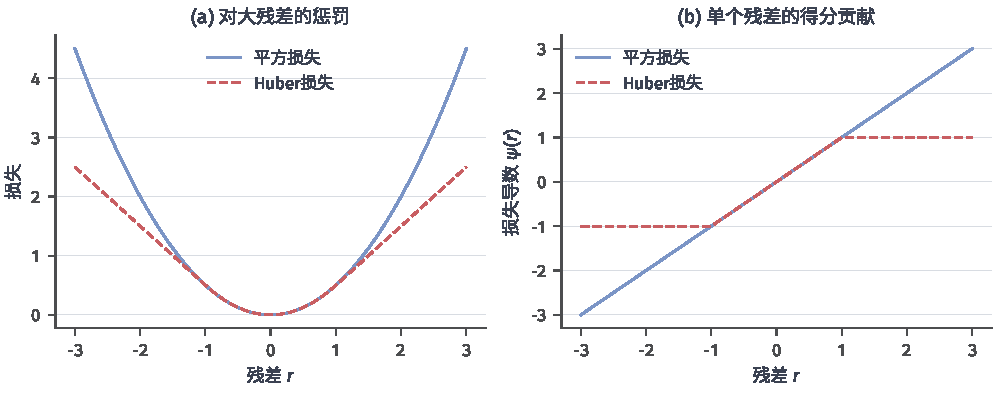
\includegraphics[width=\linewidth]{figures/01-mathematical-preliminaries/04-random-variables-distributions-and-causality/matplotlib/statistics-huber-loss/figure.pdf}
  \caption{平方损失与阈值\(c=1\)的Huber损失（解析式教学图）。左图比较惩罚值，右图比较对残差的导数；Huber得分在\([-1,1]\)内截断。横轴是构造残差，不代表实测异常值分布。}
  \label{fig:statistics-huber-loss}
\end{figure*}
% Baseline T:750-783
频率学派把参数固定而把样本看作随机。Bayes方法另给参数指定先验
\(\pi(\theta)\)，观测后用
\[
  \pi(\theta\mid\bm y)
  =
  \frac{p(\bm y\mid\theta)\pi(\theta)}
       {\int p(\bm y\mid u)\pi(u)\,\mathrm du}
\]
得到\term{后验分布}（posterior distribution）。它把似然提供的数据证据与先验
假设合并。这个公式要求分母，即模型证据，严格为正且有限；否则右侧不能定义概率分布。

对式~\eqref{eq:statistics-missing-likelihood}中的两组参数，若先验还满足
\(\pi(\theta,\psi)=\pi_\Theta(\theta)\pi_\Psi(\psi)\)，则联合后验的未归一化密度分成
\[
 \{L_{\mathrm{data}}(\theta)\pi_\Theta(\theta)\}
 \{g_\psi(\bm r\mid\bm z_{\mathrm{obs}})\pi_\Psi(\psi)\}.
\]
在归一化常数严格为正且有限时，对\(\psi\)积分只产生与\(\theta\)无关的常数，
所以关于\(\theta\)的后验也可省去机制因子。这就是Bayes分析还需要先验可分离的含义；
若先验把两组参数联系起来，该因子一般会通过\(\psi\)影响\(\theta\)的后验\scite{pgm-parameter-learning-rubin1976}

后验二阶矩有限时，后验均值最小化后验平方损失。事实上，对任意行动\(a\)，令
\(m=\mathbb{E}[\theta\mid\bm y]\)，则
\[
  \mathbb{E}[(\theta-a)^2\mid\bm y]
  =\operatorname{Var}(\theta\mid\bm y)+(a-m)^2.
\]
后验一阶绝对矩有限时，后验中位数则最小化后验绝对损失，其理由与前文总体中位数的左右方向导数相同。最大后验
估计只选择相对于指定参考测度的密度峰值；非线性重参数化会引入Jacobian因子，因此峰值
位置一般不保持不变。三种Bayes行动不必相同。

设
\[
  Y_i\mid\theta\overset{\mathrm{iid}}{\sim}\mathcal N(\theta,\sigma^2),
  \qquad
  \theta\sim\mathcal N(\mu_0,\tau_0^2).
\]
配方后得到共轭更新
\[
  \theta\mid\bm y
  \sim\mathcal N(\mu_n,\tau_n^2),\qquad
  \tau_n^{-2}=\tau_0^{-2}+n\sigma^{-2},
\]
\[
  \mu_n=\tau_n^2
  \left(\frac{\mu_0}{\tau_0^2}+\frac{n\overline y}{\sigma^2}\right).
\]
后验均值是先验均值与样本均值按精度加权的折中。新读数的后验预测还须加上观测噪声，见第~\ref{sec:statistics-scoring-calibration}节。
% Baseline T:792-834

离散比例也有同样的共轭结构。若
\(Y_i\mid p\overset{\mathrm{iid}}{\sim}\operatorname{Bernoulli}(p)\)且
\(p\sim\operatorname{Beta}(a,b)\)，观察到\(s=\sum_iY_i\)个成功后，
\[
  p\mid\bm y\sim\operatorname{Beta}(a+s,b+n-s).
\]
对\(K\)类计数\((n_1,\ldots,n_K)\)，Dirichlet先验
\(\operatorname{Dirichlet}(\alpha_1,\ldots,\alpha_K)\)相应更新为
\(\operatorname{Dirichlet}(\alpha_1+n_1,\ldots,\alpha_K+n_K)\)。这些更新依赖
给定比例后的条件独立抽样；过度离散或来源相关时，简单加计数会夸大信息量。

\par\medskip\noindent\textbf{层次模型与部分汇聚}\quad
多个设备、标注者或任务的数据量很不均衡时，可令
\[
  \theta_g\mid\mu,\tau^2\sim\mathcal N(\mu,\tau^2),\qquad
  Y_{g,i}\mid\theta_g\sim\mathcal N(\theta_g,\sigma_g^2).
\]
这里假设给定\((\mu,\tau^2)\)后各组参数\(\theta_g\)条件独立，并且给定全部组参数后，
所有\(Y_{g,i}\)也条件独立。若\(\mu,\tau^2,\sigma_g^2\)暂视为已知，且第\(g\)组有
\(n_g\)个观测，则
\[
  \theta_g\mid\bm y_g,\mu,\tau^2
  \sim\mathcal N(m_g,V_g),\qquad
  V_g^{-1}=\tau^{-2}+n_g\sigma_g^{-2},
\]
\[
  m_g
  =V_g\left(\frac{\mu}{\tau^2}
    +\frac{n_g\overline y_g}{\sigma_g^2}\right).
\]
固定超参数时，第\(g\)组后验只依赖\(\bm y_g\)以及外部给定的共同中心和尺度；
小样本群组会更强地向共同中心\(\mu\)收缩，其他组数据尚未进入该后验。
当用全部群组数据估计共同超参数，或在完整Bayes模型中对其后验积分时，其他组数据才会
通过共同超参数间接改变第\(g\)组的推断，从而形成组间信息共享。
\(\tau^2\to0\)接近完全汇聚，\(\tau^2\to\infty\)接近各组独立估计，有限正尺度给出
部分汇聚。若超参数由同一数据估计，这是经验Bayes；若继续给它们指定先验，推断对象还
包括超参数后验。
这不是免费增加数据，而是加入“群组来自共同总体”的结构假设。若群组机制不同或先验
尺度过窄，收缩会掩盖真实差异。先验由研究者指定并不把固定物理参数变成随机生成的
事实；Bayes概率表达的是模型内部的不确定性。
对于有限个分位数，经验分布
\(\widehat F_n(y)=n^{-1}\sum_i\mathbb I_{\{Y_i\leq y\}}\)的广义逆给出
\(\widehat q=Y_{(\lceil nq\rceil)}\)。它估计的是总体分位数，不是未来读数的覆盖阈值；后者在共形预测中使用不同的秩修正。若总体在目标分位附近严格越过水平\(q\)，经验分布的统一收敛保证该估计一致；平坦区间、原子与不唯一目标则需按所选分位约定分析。

\subsubsection{分布与条件函数的估计}
\label{sec:statistics-nonparametric-missing}
经验分布把每个样本点赋质量\(1/n\)，因而是完整的概率分布而不是密度曲线。独立同分布样本下，Glivenko--Cantelli定理给出
\(\sup_y|\widehat F_n(y)-F(y)|\to0\)几乎必然；固定\(y\)的大数定律本身尚不等于这个统一结论。参数化方法则可报告\(P_{\widehat\theta}\)，例如
\(\mathcal N(\overline Y,S^2)\)，其有效性另外依赖模型限制。下面的平滑表示改变了分布或条件函数的形状，需要同时控制逼近误差与局部样本波动。
% Baseline T:1474-1583
有限维模型可能把真实分布限制得过强。非参数方法不预先固定有限个参数，但仍通过带宽、
邻域或平滑度控制复杂度。以下令\(Y_1,\ldots,Y_n\)独立同分布，具有同一个一维
密度\(f\)，并采用不依赖本批观测的带宽\(h=h_n>0\)。相关、选择或加权样本
需要另行计算期望与协方差，不能直接使用下面的独立样本公式。给定宽度为\(h\)的分箱，直方图用
“箱内样本数除以\(nh\)”作为箱内常数密度；移动箱边界可能改变估计。核密度估计则把
每个样本扩散为核：
\[
  \widehat f_h(x)
  =\frac1{nh}\sum_{i=1}^n
    K\left(\frac{x-Y_i}{h}\right).
\]
若\(K\geq0\)、积分为\(1\)，则\(\widehat f_h\)本身是非负且积分为\(1\)的密度。
为直接使用局部Taylor展开，以下采用一组充分条件：\(K\)有界、紧支撑且对称，
二阶矩记为\(\mu_2(K)=\int u^2K(u)\,\mathrm du\)，并记
\(R(K)=\int K(u)^2\,\mathrm du\)；两者均有限。设\(f\)在内部点\(x\)的邻域
二阶连续可微，则小带宽下核只涉及这个光滑邻域，由
\[
  \mathbb{E}[\widehat f_h(x)]
  =\int K(u)f(x-hu)\,\mathrm du
\]
作Taylor展开，核的一阶矩因对称性消失，从而得到
\[
  \operatorname{Bias}\{\widehat f_h(x)\}
  =\frac{h^2\mu_2(K)}2f''(x)+o(h^2),
\]
\[
  \operatorname{Var}\{\widehat f_h(x)\}
  =\frac{f(x)R(K)}{nh}+o((nh)^{-1}),
\]
其中渐近式取\(h\to0\)、\(nh\to\infty\)。较大带宽降低方差却增加平滑偏差。
边界附近因核质量落到支持集外，上述对称展开失效。
在\(d\)维中，体积因子变为\(h^d\)，代表性点态方差阶数相应为
\(1/(nh^d)\)。因此维数增加会更快消耗局部样本；一维的带宽结论不能不改条件直接
移植到高维。

\par\medskip\noindent\textbf{局部预测与近邻}\quad
这里的观测改为\((X_i,Y_i)_{i=1}^n\)，假定它们来自同一联合分布且独立同分布，
\(Y\)可积。采用前面核密度估计中的非负、有界、紧支撑核\(K\)与确定带宽\(h>0\)。
回归函数\(m(x)=\mathbb{E}[Y\mid X=x]\)可由局部平均估计；以下比值只在
权重和\(\sum_iK((X_i-x)/h)>0\)时定义：
\[
  \widehat m_h(x)=
  \frac{\sum_iK((X_i-x)/h)Y_i}
       {\sum_iK((X_i-x)/h)}.
\]
局部线性回归在\(x\)附近拟合\(a+b(X_i-x)\)，在相应平滑条件下可减轻设计
密度不均和边界偏差。下面的唯一拟合还要求局部加权设计满秩；在这个一维两参数问题中，
即正权重的输入至少含两个不同取值。若权重和为零或设计退化，需扩大邻域或另给退化处理，
不能照用比值或逆矩阵公式。
\[
  (\widehat a,\widehat b)
  \in\argmin_{a,b}\sum_{i=1}^n
  K\left(\frac{X_i-x}{h}\right)
  \{Y_i-a-b(X_i-x)\}^2,
  \qquad \widehat m_{\mathrm{local}}(x)=\widehat a.
\]
\(k\)近邻取\(1\leq k\leq n\)，用离\(x\)最近的\(k\)个样本平均；距离并列时
按预先指定的规则选择。维数增大时，为包含足够邻居必须扩大
邻域，Taylor局部性随之变差，这就是维数灾难的一种表现。

在例~\ref{ex:statistics-running-sensor-calibration}的左边界\(x_0=0\)，局部常数
估计为
\[
  \widehat m_h(0)
  =
  \frac{1\times9+0.75\times11+0.25\times13}
       {1+0.75+0.25}
  =10.25.
\]
局部线性拟合令\(u_i=x_i-x_0\)。由这三个点可算得
\[
  S_0=\sum_i w_i=2,\quad
  S_1=\sum_i w_i u_i=1.5,\quad
  S_2=\sum_i w_i u_i^2=3,
\]
\[
  T_0=\sum_i w_i y_i=20.5,\qquad
  T_1=\sum_i w_i u_i y_i=18.
\]
加权正规方程给出
\[
  \widehat a
  =\frac{S_2T_0-S_1T_1}{S_0S_2-S_1^2}
  =9.2,\qquad
  \widehat b
  =\frac{S_0T_1-S_1T_0}{S_0S_2-S_1^2}
  =1.4.
\]
因此局部线性预测为\(9.2\)，而局部常数预测为\(10.25\)。在边界处，后者只能对单侧
观测加权平均，前者还估计局部斜率并把直线截距放回\(x_0\)；哪一个更接近真实条件均值
仍取决于局部线性近似和带宽是否合适，不能由这一组数值单独决定。

图~\ref{fig:statistics-local-boundary-fit}显示这两个预测值的几何区别：水平线只改变高度，斜线同时解释输入位置与响应的局部变化，再把截距取回边界点。图中的观测和权重就是上面的三个教学数据；未画出未知的真实条件均值，因此不能从图上断言哪一种估计误差更小。
\begin{figure}[htbp]
  \centering
  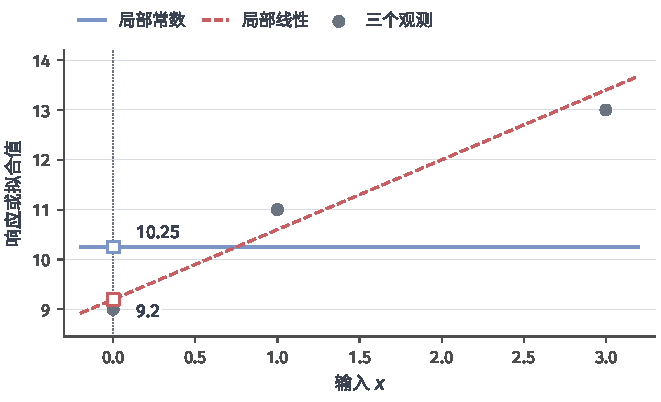
\includegraphics[width=\linewidth]{figures/01-mathematical-preliminaries/04-random-variables-distributions-and-causality/matplotlib/statistics-local-boundary-fit/figure.pdf}
  \caption{边界处的局部常数与局部线性拟合（教学数据图）。观测为\((0,9),(1,11),(3,13)\)，权重为\(1,0.75,0.25\)。蓝实线为加权常数\(10.25\)，红虚线为\(9.2+1.4x\)，边界\(x_0=0\)处分别预测\(10.25\)和\(9.2\)。}
  \label{fig:statistics-local-boundary-fit}
\end{figure}

在上述独立同分布抽样下，这些方法的一致性需要邻域既缩小又包含越来越多样本。
例如一维内部点处，若输入密度在
\(x\)附近连续且为正，条件均值足够光滑，条件方差局部有界，并取
\(h\to0\)、\(nh\to\infty\)，局部常数估计的平滑偏差消失，局部平均的方差也消失。
输入密度与条件均值都二阶连续可微时，常用局部展开给出\(O(h^2)\)的平滑偏差
以及\(O((nh)^{-1})\)的方差，因此平滑偏差的平方为\(O(h^4)\)；精确常数还依赖
核、输入密度与条件噪声。近邻版本相应要求\(k\to\infty\)且\(k/n\to0\)。
这些都是目标分布有局部覆盖时的内插结论；在训练输入密度为零的区域，缩小邻域无法产生
新信息，外推保证必须来自额外结构假设。
% Baseline T:977-988
条件分位数可由\term{分位数回归}估计。假设\(Y\)可积，使下面损失的条件期望对几乎每个\(x\)有限。令
\[
  \rho_q(u)=u\bigl(q-\mathbb{I}_{\{u<0\}}\bigr),
\]
则条件\(q\)分位数最小化
\(\mathbb{E}[\rho_q(Y-a)\mid X=x]\)。固定\(x\)并记条件分布函数为\(F\)，目标对
\(a\)的次梯度区间是
\[
  [F(a^-)-q,\ F(a)-q].
\]
因此最优点恰好满足\(F(a^-)\leq q\leq F(a)\)；连续严格递增时才简化为
\(F(a)=q\)。因此分位数损失的最小点集合正是\(\mathcal Q_q\)，可能不唯一，
而\(F^{-1}(q)\)仍是其中按约定选出的单个代表。分位数回归直接估计条件分布的位置，
不要求误差为高斯或方差恒定。
实际分位数回归把条件分位函数写成\(a=f(x)\)，最小化
\(\sum_i\rho_q(Y_i-f(X_i))\)及可能的正则项。线性、样条或其他函数类限制决定了可表示的条件分位形状；最小化同一损失不意味着所有表示有同样的偏差与覆盖保证。

\subsection{未观测结果的预测}
\label{sec:stats-prediction-observation-limits}
估计未知均值以后，新观测仍有自身噪声。平方损失下的点预测是预测分布的均值，绝对损失下是中位数；二元错判损失下选择概率较大的类别。先给出预测分布，再按损失选择一个点或一组允许值，才能避免把参数精度误当成结果精度。

\subsubsection{预测分布与概率评价}
\label{sec:statistics-scoring-calibration}
若参数给定，条件预测使用概率核\(P_\theta(Y_{\rm new}\in\cdot\mid X_{\rm new}=x)\)；
代入估计得到插件预测，Bayes方法则对参数后验积分：
\[
P(Y_{\rm new}\in A\mid\bm y,x)
=\int P_\theta(Y_{\rm new}\in A\mid x)\,\pi(\mathrm d\theta\mid\bm y),
\]
这里假设给定参数后新观测与训练数据按模型条件独立。代入一个参数通常没有传播全部参数不确定性。
在前述高斯共轭模型中，
% Baseline T:784-790
\[
  Y_{n+1}\mid\bm y
  \sim\mathcal N(\mu_n,\sigma^2+\tau_n^2).
\]
其中\(\tau_n^2\)是参数不确定性，\(\sigma^2\)是新观测自身的噪声。
% Baseline T:1358-1467
点预测只给一个结果，概率预测则给出整个候选分布。若只奖励是否猜中最可能结果，报告完整概率并没有优势；评分必须鼓励把真实不确定性如实报告。
\begin{definition}[适当评分规则]
  \label{def:statistics-proper-scoring-rule}
  给定预测分布类\(\mathcal P\)，\term{评分规则}（scoring rule）\(S(Q,y)\)，即报告预测分布\(Q\)而结果为\(y\)
时承担的损失。假定所比较的期望均有定义，且诚实报告的期望有限。若对每个\(P,Q\in\mathcal P\)有\(\mathbb E_PS(P,Y)\leq\mathbb E_PS(Q,Y)\)，就称评分规则
\term{适当}（proper）；若适用分布类中的最小点唯一，则称为严格适当。
\end{definition}
它奖励诚实概率，而不是只检查最可能类别是否猜中。

先考虑有限结果集\(\mathcal Y\)，并记\(P,Q\)的概率质量函数为\(p,q\)。本节只需
有限离散情形的\term{KL散度}（Kullback--Leibler divergence）：
\[
  D_{\mathrm{KL}}(P\Vert Q)
  =
  \sum_{y\in\mathcal Y}p(y)\log\frac{p(y)}{q(y)}.
\]
其中约定\(0\log(0/q)=0\)；只要存在\(p(y)>0\)而\(q(y)=0\)，就令散度为
\(+\infty\)。由\(-\log u\geq1-u\)可得
\(D_{\mathrm{KL}}(P\Vert Q)\geq0\)，等号当且仅当\(P=Q\)。
这也可看成对凸函数\(-\log\)应用Jensen不等式：在\(P\)的支持上平均
\(q(y)/p(y)\)，所得总和不超过\(1\)。
第~\ref{chap:information-theory-and-statistical-geometry}章将在一般测度空间上定义
这一量，并系统讨论其性质。

离散结果的对数评分为\(S(Q,y)=-\log q(y)\)。根据上述定义，其期望差满足
\[
  \mathbb{E}_P[S(Q,Y)]-\mathbb{E}_P[S(P,Y)]
  =\sum_{y\in\mathcal Y}p(y)\log\frac{p(y)}{q(y)}
  =D_{\mathrm{KL}}(P\Vert Q)\geq0.
\]
因此对数评分是严格适当的；零预测概率遗漏真实分布的支持时，期望损失为无穷。
连续密度版本还要求相对于共同参考测度定义密度，并保证相关对数期望有定义；改变参考
坐标会改变单个对数密度值，但在合法换元下比较同一结果分布的期望差保持一致。

二元结果\(Y\in\{0,1\}\)的Brier评分为\(S(q,Y)=(q-Y)^2\)。若真实事件概率为
\(p\)，则
\begin{align}
  \mathbb{E}_p[(q-Y)^2]
  &=p(q-1)^2+(1-p)q^2\\
  &=(q-p)^2+p(1-p).
\end{align}
第二项与报告\(q\)无关，所以唯一最优报告是\(q=p\)。对数评分更强烈惩罚对已发生
事件给极小概率，Brier评分则有界；两者表达不同风险偏好。

对\(K\)个类别，令真实概率向量为\(\bm p\)，报告为\(\bm q\)，Brier评分可写成
\(S(\bm q,Y)=\sum_{k=1}^K(q_k-\mathbb{I}\{Y=k\})^2\)。直接展开得到
\[
  \mathbb{E}_{\bm p}[S(\bm q,Y)]
  =\lVert\bm q-\bm p\rVert_2^2
   +1-\lVert\bm p\rVert_2^2.
\]
所以它在概率单纯形上同样严格适当，但控制的是概率向量的平方距离，不是对数密度比。

\par\medskip\noindent\textbf{校准、区分能力与锐度}\quad
\begin{definition}[二元概率校准]
  \label{def:statistics-probability-calibration}
  设\(Y\in\{0,1\}\)，预测概率为随机变量\(Q\in[0,1]\)。若
  \[ \mathbb E[Y\mid Q]=Q\quad\text{几乎必然}, \]
  则称预测相对于当前联合总体分布是\term{校准}（calibration）的。等价地，\(\mathbb P(Y=1\mid Q=q)=q\)对\(P_Q\)-几乎每个\(q\)成立。
\end{definition}
它要求预测概率相同的一组样本具有相应的真实发生率，而不要求有限样本中每组频数恰好等于预测值。\term{区分能力}（discrimination）描述模型
能否给更可能发生事件的样本更高分；\term{锐度}（sharpness）描述预测分布是否集中。
对所有样本恒报基准发生率可以完美校准，却没有区分能力。锐度只有在校准前提下才值得
追求。

令\(Q=\widehat p(X)\)、\(\eta(Q)=\mathbb{E}[Y\mid Q]\)，再记总体发生率为
\(\overline p=\mathbb{E}[Y]\)。条件平方展开给出
\[
  \mathbb{E}[(Q-Y)^2]
  =
  \underbrace{\mathbb{E}[(Q-\eta(Q))^2]}_{\text{校准误差}}
  +\underbrace{\overline p(1-\overline p)
    -\operatorname{Var}(\eta(Q))}_{\text{剩余不可分辨误差}}.
\]
第一项为零才表示相对于预测值本身校准；第二项随不同预测组的真实风险更可区分而减小。
恒报\(\overline p\)使第一项为零，却也使
\(\operatorname{Var}(\eta(Q))=0\)。多类别校准相应要求
\(\mathbb{P}(Y=k\mid\widehat{\bm p})=\widehat p_k\)对每个类别成立，逐类别边际校准
通常弱于这个向量条件。

一个固定的两组例子可以把这几个性质分开。设两组各占总体一半，事件概率分别为\(0.2,0.8\)。如表~\ref{tab:statistics-calibration-discrimination}，恒报\(0.5\)和按组报\(0.2,0.8\)都校准；前者把两组混在一起，后者保留了风险差异。按组报\(0,1\)保持相同排序，预测更集中，却把仍可能发生的意外结果说成不可能。
\begin{table}[htbp]
  \centering
  \small
  \begin{tabular}{lccc}
    \toprule
    报告规则 & 两组概率 & 总体校准 & 期望Brier损失 \\
    \midrule
    恒报总体发生率 & \(0.5,0.5\) & 是 & \(0.25\) \\
    如实报告组风险 & \(0.2,0.8\) & 是 & \(0.16\) \\
    只保留确定类别 & \(0,1\) & 否 & \(0.20\) \\
    \bottomrule
  \end{tabular}
  \caption{同一个两组总体下的校准与区分能力。数值由\(\mathbb E[(q-Y)^2]=(q-p)^2+p(1-p)\)逐组平均得到；后两行的类别排序相同，但概率准确性不同。}
  \label{tab:statistics-calibration-discrimination}
\end{table}

\par\medskip\noindent\textbf{后处理校准与评价条件}\quad
温度缩放对分类logit \(\bm z\)使用
\(\operatorname{softmax}(\bm z/T)\)，在校准集上按对数损失估计\(T>0\)。它保持
类别排序，只调整置信程度。保序回归则拟合单调的分数到概率映射，更灵活但更容易在小
校准集上过拟合。给定排序分数\(s_i\)，其典型拟合问题是在
\(q_1\leq\cdots\leq q_m\)约束下最小化
\(\sum_i(q_i-y_i)^2\)；单调约束不等于总体校准保证。
训练原预测器、拟合校准器和评价校准效果应使用职责分离的数据或严格的折外预测；
部署总体若发生变化，旧映射也未必保持校准。分箱可靠性图只是把连续条件近似成有限组，
箱内比例仍有抽样误差，且结果依赖分箱边界。适当评分、边际覆盖和校准分别评价分布损失、
未来集合与条件发生率，不能互相替代。

\subsubsection{预测集合与覆盖}
\label{sec:probability-exchangeability-conformal-ranks}
\label{sec:rv-prediction-sets}
预测集合\(C(\bm Y)\)在规定的训练数据与未来观测联合规律下要求
\(\mathbb P\{Y_{n+1}\in C(\bm Y)\}\geq1-\alpha\)，其中\(0<\alpha<1\)。
在独立高斯位置模型\(Y_i\sim\mathcal N(\theta,\sigma^2)\)且\(\sigma\)已知时，
\[
Y_{n+1}-\overline Y\sim\mathcal N(0,\sigma^2(1+1/n)).
\]
因为新噪声与训练均值独立，方差中除了估计均值的\(\sigma^2/n\)，还有新观测的\(\sigma^2\)。因此
\[
C(\bm Y)=\left[\overline Y-z_{1-\alpha/2}\sigma\sqrt{1+1/n},
\overline Y+z_{1-\alpha/2}\sigma\sqrt{1+1/n}\right].
\]
这里\(z_p\)是标准高斯分布的下\(p\)分位数。取\(1-\alpha=0.95\)，
例~\ref{ex:statistics-running-sensor-calibration}的数值给出
\([6.40,14.40]\)。方差未知但仍为高斯独立样本时，可用
\(\overline Y\pm t_{n-1,1-\alpha/2}S\sqrt{1+1/n}\)获得精确预测区间。
其中\(n\geq2\)，\(S^2=(n-1)^{-1}\sum_i(Y_i-\overline Y)^2\)，
\(t_{\nu,p}\)为自由度\(\nu\)的Student \(t\)分布下\(p\)分位数。
该分布是独立的\(Z\sim\mathcal N(0,1)\)与\(U\sim\chi_\nu^2\)所成比值
\(Z/\sqrt{U/\nu}\)的规律。要在这里使用它，须把样本分成独立的均值方向和残差方向。

\begin{lemma}[高斯样本的均值与残差分解]
\label{lem:statistics-gaussian-mean-residual}
设\(n\geq2\)、\(\sigma>0\)，且\(Y_1,\ldots,Y_n\)独立同分布于
\(\mathcal N(\theta,\sigma^2)\)。则
\[
 Z_0=\frac{\sqrt n(\overline Y-\theta)}{\sigma}\sim\mathcal N(0,1),
 \qquad U=\frac{(n-1)S^2}{\sigma^2}\sim\chi^2_{n-1},
\]
且\(Z_0\)与\(U\)独立。
\end{lemma}
\begin{proof}
将标准化样本写成\(\bm\varepsilon=(\bm Y-\theta\bm1)/\sigma\sim\mathcal N(\bm0,\bm I_n)\)。
选择首行为\(\bm1^\top/\sqrt n\)的正交矩阵\(\bm Q\)；其余行构成与\(\bm1\)正交的残差方向。
向量\(\bm V=\bm Q\bm\varepsilon\)仍服从\(\mathcal N(\bm0,\bm I_n)\)，
所以各坐标是独立标准高斯。第一坐标\(V_1=Z_0\)；
正交变换保持长度，并把常量方向与其正交补分开，故
\[
 \sum_{j=2}^nV_j^2
 =\left\|\bm\varepsilon-\frac{\bm1\bm1^\top}{n}\bm\varepsilon\right\|_2^2
 =\frac1{\sigma^2}\sum_{i=1}^n(Y_i-\overline Y)^2=U.
\]
因此残差平方和具有\(n-1\)个自由度，并与第一坐标独立。
\end{proof}
新观测\(Y_{n+1}\)独立于全部训练样本，所以\((Y_{n+1},\overline Y)\)与\(S\)独立，
且\((Y_{n+1}-\overline Y)/(\sigma\sqrt{1+1/n})\)是标准高斯。
将它与上述\(U\)代入\(t\)分布定义，就得到所用的精确预测区间。
这类保证依赖参数模型；只愿假设可交换性时，可改用下面的秩方法。
% Baseline P:2293-2356
设实值分数\(S_1,\ldots,S_{m+1}\)可交换，并暂假它们几乎必然没有并列值。令
\[ R_{m+1}
  =1+\sum_{i=1}^{m}\mathbb{I}\{S_i<S_{m+1}\} \]
为最后一个分数从小到大的秩。由于交换任意两个坐标不改变联合分布，而无并列值时每个样本恰占一个秩，所以
\begin{equation}
  \mathbb{P}(R_{m+1}=r)=\frac{1}{m+1},
  \qquad r=1,\ldots,m+1.
  \label{eq:probability-uniform-rank}
\end{equation}
这是一项精确的有限样本结论，不依赖中心极限定理。

若存在并列值，使用“严格小于”的秩不再均匀。可以为每个分数附加独立连续随机数并按字典序打破并列，此时恢复精确均匀秩；也可以采用保守的不随机化分位数，得到覆盖率至少为目标值，但通常不再精确等于目标值。

\par\medskip\noindent\textbf{拆分共形预测的有限样本覆盖}\quad
设训练数据用于拟合一个固定预测规则，随后有\(m\)个校准样本和一个未来样本。条件于训练数据，假设校准样本与未来样本可交换。用同一个不一致性函数计算
\[ S_i=s(X_i,Y_i),
  \qquad i=1,\ldots,m+1. \]
分数越大表示候选标签与预测规则越不相容。给定错误率\(\alpha\in(0,1)\)，令
\[ k=\left\lceil(m+1)(1-\alpha)\right\rceil. \]
若\(k\leq m\)，令\(q\)为前\(m\)个校准分数的第\(k\)小值；若\(k=m+1\)，约定\(q=+\infty\)。对新输入\(X_{m+1}\)，定义预测集合
\begin{equation}
  C(X_{m+1})
  =
  \{y:s(X_{m+1},y)\leq q\}.
  \label{eq:probability-split-conformal-set}
\end{equation}

例如\(m=9\)、\(\alpha=0.2\)时，\(k=\lceil10\times0.8\rceil=8\)。若排序后的校准分数为
\(0.1,0.2,\ldots,0.9\)，则\(q=0.8\)：候选标签的分数为\(0.75\)时纳入集合，为\(0.85\)时排除。若仍只有九个校准样本却要求
\(\alpha=0.05\)，则\(k=\lceil9.5\rceil=10=m+1\)，按约定得到\(q=+\infty\)。这不是计算故障，而是有限样本不足以用非随机秩给出如此高的非平凡覆盖水平。

\begin{theorem}[拆分共形的有限样本覆盖]
\label{thm:probability-split-conformal-coverage}
在上述条件下，
\[ \mathbb{P}\bigl(
    Y_{m+1}\in C(X_{m+1})\bigr)\geq 1-\alpha. \]
\end{theorem}

\begin{proof}
先假设分数无并列值。若未来真实标签未被覆盖，则\(S_{m+1}>q\)，所以未来分数在全部\(m+1\)个分数中的秩严格大于\(k\)。由式~\eqref{eq:probability-uniform-rank}，
\[ \mathbb{P}(S_{m+1}>q)
  =\mathbb{P}(R_{m+1}>k)=\frac{m+1-k}{m+1}\leq\alpha. \]
取补事件即得覆盖结论。

若有并列值，采用集合定义中的“\(\leq q\)”会把边界并列分数纳入预测集合。相较于随机打破并列后的精确秩，这只会增加覆盖事件，因此同一不等式仍成立。若希望得到更接近
精确的覆盖率，可显式随机化边界并列项，但必须把该随机化纳入算法与概率空间。
\end{proof}

这里的概率保证是\term{边际覆盖}：条件于训练数据后，它仍对随机的校准样本和未来样本共同取平均；若采用随机并列处理，还包括该随机性。解除对训练数据的条件后，总体覆盖率仍至少为
\(1-\alpha\)。但这个结论一般不推出对每个固定输入\(x\)都有
\[
  \mathbb{P}\bigl(
    Y_{m+1}\in C(X_{m+1})
    \mid X_{m+1}=x
  \bigr)
  \geq1-\alpha,
\]
也不自动保证每个群组内都达到同一覆盖率。逐输入、逐群组或时间条件覆盖需要额外结构、假设或专门的校准方法，不能仅由可交换秩推出。

证明依赖两处对称性。训练与校准拆分使评分规则在校准阶段保持固定；校准样本与未来样本可交换，使未来分数的秩没有特殊位置。若反复查看校准误差后修改模型或分数函数，评分规则
已依赖校准标签，条件可交换性可能被破坏。时间序列中的未来点通常也不能与过去点任意重排；自适应收集会让被选中的样本位置携带额外信息。此时失效的是均匀秩步骤，而不是把
分位数索引稍作调整就能修复。\BookSectionRef{sec:reliability-guarantee}
{第二卷“基础、理论和可信性”的“可靠性的保证”节}建立具体预测范围后，将回用这一秩保证。
分组校准需要在看见校准结果前规定群组，并有足够的组内可交换样本。边际覆盖平均了输入位置，不自动给出每个连续输入处的条件覆盖。

\subsection{推断误差与假设检验}
\label{sec:stats-uncertainty-testing-selection}
估计值用风险评价，参数范围用覆盖评价，候选命题用拒绝错误评价。Bootstrap与置换分别服务于这些输出；数据选择与持续查看则改变结论的产生规则，必须进入保证的条件。

\subsubsection{估计误差与效率}
\label{sec:statistics-bias-efficiency}
% Baseline T:446-459
估计量的误差既来自系统偏移，也来自样本波动。对标量目标\(\theta\)，
\begin{align}
  \mathbb{E}[(\widehat\theta-\theta)^2]
  &=
  \mathbb{E}[(\widehat\theta-\mathbb{E}\widehat\theta
  +\mathbb{E}\widehat\theta-\theta)^2] \notag\\
  &=
  \operatorname{Var}(\widehat\theta)
  +\bigl(\mathbb{E}[\widehat\theta]-\theta\bigr)^2.
  \label{eq:statistics-mse-decomposition}
\end{align}
交叉项期望为零，因而均方误差等于方差加偏差平方。无偏不等于误差最小；少量偏差可能
换来更大的方差下降。

% Baseline T:470-498
若\(\bm\theta\in\mathbb{R}^d\)并使用总平方误差，则
\[
  \mathbb{E}\lVert\widehat{\bm\theta}-\bm\theta\rVert_2^2
  =\operatorname{tr}\{\operatorname{Cov}(\widehat{\bm\theta})\}
   +\lVert\mathbb{E}\widehat{\bm\theta}-\bm\theta\rVert_2^2.
\]
这不是每个坐标风险的最大值，也不是任意方向风险。

在高斯位置例子中，取固定中心\(\mu_0\)并令
\(\widetilde\theta=a\overline Y+(1-a)\mu_0\)，则
\[
  \operatorname{MSE}_\theta(\widetilde\theta)
  =\frac{a^2\sigma^2}{n}+(1-a)^2(\mu_0-\theta)^2.
\]
当\(\theta\)接近\(\mu_0\)时，某些\(a<1\)可比无偏的样本均值具有更小有限样本
均方误差；远离中心时，收缩偏差又可能占主导。比较结论必须固定目标、样本量和损失。

当任意\(\epsilon>0\)都满足
\(\mathbb{P}_\theta(|\widehat\theta_n-\theta|>\epsilon)\to0\)时，称估计量
\term{一致}（consistent）。一致性只描述样本量趋于无穷的极限，不给出当前样本的
误差，也不排除有限样本偏差。若
\(\mathbb{E}_\theta[(\widehat\theta_n-\theta)^2]\to0\)，则称为均方一致；
Markov不等式说明均方一致推出依概率一致，反向结论没有额外一致可积性时并不成立。
对某些满足额外正则条件的估计量，还能进一步证明
\[
  \sqrt n(\widehat\theta_n-\theta)
  \xrightarrow{\mathrm d}\mathcal N(0,V).
\]
这项性质称为渐近正态，它需要另行建立，并不由一致性自动推出。
% Baseline T:516-547
无偏性约束了平均位置，却尚未比较方差。把单一信号推广为一组带噪线性观测：给定设计矩阵\(\bm X\in\mathbb R^{n\times d}\)，设
\begin{equation}
  \bm Y=\bm X\bm\theta+\bm\varepsilon,\qquad
  \mathbb E[\bm\varepsilon\mid\bm X]=\bm0,\qquad
  \operatorname{Cov}(\bm\varepsilon\mid\bm X)=\sigma^2\bm I_n,
  \quad\sigma^2>0.
  \label{eq:statistics-gauss-markov-model}
\end{equation}
不同观测的条件噪声方差相同且协方差为零；这里不要求独立或高斯噪声。列满秩使参数可识别，第~\ref{chap:linear-algebra}章的最小二乘解为
\(\widehat{\bm\theta}=(\bm X^\top\bm X)^{-1}\bm X^\top\bm Y\)。它是否在所有无偏估计中最佳，需要先限定比较类。
\begin{theorem}[Gauss--Markov定理]
  \label{thm:statistics-gauss-markov}
  在式~\eqref{eq:statistics-gauss-markov-model}下，若\(\bm X\)列满秩，则\(\widehat{\bm\theta}\)条件无偏，且
  \(\operatorname{Cov}(\widehat{\bm\theta}\mid\bm X)=\sigma^2(\bm X^\top\bm X)^{-1}\)。
  对任何条件于\(\bm X\)固定、对全部\(\bm\theta\)均无偏的线性估计\(\widetilde{\bm\theta}=\bm C\bm Y\)，有
  \[
    \operatorname{Cov}(\widetilde{\bm\theta}\mid\bm X)
    -\operatorname{Cov}(\widehat{\bm\theta}\mid\bm X)\succeq\bm0.
  \]
\end{theorem}
\begin{proof}
记\(\bm C_0=(\bm X^\top\bm X)^{-1}\bm X^\top\)，于是\(\bm C_0\bm X=\bm I_d\)。直接对\(\bm C_0\bm Y\)求条件均值和协方差，得到无偏性及所述协方差。任一线性估计对所有参数无偏，等价于\(\bm C\bm X=\bm I_d\)。写\(\bm C=\bm C_0+\bm D\)，则\(\bm D\bm X=\bm0\)，从而
\[
  \bm C_0\bm D^\top
  =(\bm X^\top\bm X)^{-1}(\bm D\bm X)^\top=\bm0.
\]
展开\(\sigma^2\bm C\bm C^\top\)时两个交叉项都为零，故协方差之差为\(\sigma^2\bm D\bm D^\top\)。对任意向量\(\bm a\)，其二次型为\(\sigma^2\|\bm D^\top\bm a\|_2^2\geq0\)，即得半正定结论。
\end{proof}
半正定比较表示任意线性组合\(\bm a^\top\bm\theta\)的方差都不更大，强于只比较各坐标方差。定理的比较类是线性无偏估计，不排除前面那类有偏收缩估计获得更小均方误差，也不把异方差或相关噪声包含进来。

若\(\bm X=\bm1_n\)，参数就是共同均值，最小二乘退化为样本平均。任一无偏加权平均\(\sum_i a_iY_i\)满足\(\sum_i a_i=1\)；写\(a_i=1/n+b_i\)，则\(\sum_i b_i=0\)，其方差为
\(\sigma^2\sum_i a_i^2=\sigma^2/n+\sigma^2\sum_i b_i^2\)。额外的不均衡权重只增加方差，给出矩阵证明的一个可逐项核对的特例。
% Baseline T:551-560
样本均值给出渐近正态的基本例子。若
\(Y_1,\ldots,Y_n\)独立同分布，且
\(\mathbb{E}[Y_i]=\theta\)、
\(0<\operatorname{Var}(Y_i)=\sigma^2<\infty\)，则中心极限定理给出
\[
  \sqrt n(\overline Y-\theta)
  \xrightarrow{\mathrm d}\mathcal N(0,\sigma^2).
\]
因此均值的渐近正态只需要有限方差，不要求观测本身服从高斯分布；在高斯位置模型中，
这个正态分布关系对每个有限\(n\)已经精确成立。
数值极限运算使用第~\ref{sec:rv-numerical-convergence}节的Slutsky和Delta方法。例如均值的标准误估计只要依概率趋向正确尺度，就可代入相应渐近统计量；这一条件不能由标准误的数值看起来合理来代替。
% Baseline T:636-743
一般估计方程的渐近式还要控制在随机估计点附近的斜率。设\(Y_i\)独立同分布，且
\(\mathbb{E}[\psi(Y,\theta_0)]=0\)，记
\[
  A=\mathbb{E}[\partial_\theta\psi(Y,\theta_0)],
  \qquad B=\operatorname{Var}(\psi(Y,\theta_0)),
\]
要求\(A\neq0\)、\(B<\infty\)。一组足够条件是：\(\widehat\theta\)依概率趋于内点
\(\theta_0\)；\(\psi(y,\theta)\)在其某个邻域内连续可微；经验导数
\(n^{-1}\sum_i\partial_\theta\psi(Y_i,\theta)\)在该邻域上一致依概率收敛到
连续函数\(a(\theta)=\mathbb E[\partial_\theta\psi(Y,\theta)]\)；
估计方程残差\(r_n=n^{-1}\sum_i\psi(Y_i,\widehat\theta)\)满足
\(r_n=o_{\mathbb P}(n^{-1/2})\)。
一致性保证连接\(\theta_0\)与\(\widehat\theta\)的线段以趋于一的概率留在该邻域内。
沿线段积分导数，得到
\[
\begin{aligned}
 A_n&=\int_0^1\frac1n\sum_{i=1}^n
  \partial_\theta\psi\bigl(Y_i,\theta_0+t(\widehat\theta-\theta_0)\bigr)\,\mathrm dt
  \xrightarrow{\mathbb P}A,\\
 r_n&=\frac1n\sum_{i=1}^n\psi(Y_i,\theta_0)+A_n(\widehat\theta-\theta_0).
\end{aligned}
\]
随机斜率的收敛由一致导数控制与\(a\)的连续性共同给出，不能仅凭在固定点可微就断言。
因\(A\neq0\)，以趋于一的概率可以除以\(A_n\)；再由中心极限定理与Slutsky得到
\[
  \sqrt n(\widehat\theta-\theta_0)
  =
  -A^{-1}\frac1{\sqrt n}\sum_{i=1}^n\psi(Y_i,\theta_0)
  +o_{\mathbb{P}}(1),
\]
故极限方差为\(A^{-2}B\)，\(B=0\)时极限退化为零。多维情形将导数换为Jacobian，
要求其总体矩阵\(A\)非奇异，并对向量得分使用多元中心极限定理；极限协方差相应为
\(A^{-1}B(A^{-1})^\top\)，常称夹心协方差。模型正确的光滑似然在正则条件下可用
信息恒等式化简它；模型失配时\(A\)与\(B\)通常不再是同一个信息量，夹心两侧不能省略。

\par\medskip\noindent\textbf{得分、Fisher信息与效率界}\quad
均方误差评价一个给定估计量，效率界进一步询问同一观测模型允许的估计精度。
这里用对数似然的导数记录数据对参数的局部辨别能力；Fisher信息与统计几何章共用
同一个分布对象，本小节将它用于无偏估计的误差下界，而非另建一种曲率矩阵。

\term{Fisher信息}（Fisher information）衡量观测分布对参数局部变化的敏感程度。

\begin{definition}[Fisher信息矩阵]
\label{def:information-fisher-matrix}
对开参数域上的受共同测度支配模型\(p_{\bm\theta}\)，固定参数内点\(\bm\theta\)。假设在\(P_{\bm\theta}\)-几乎每个\(x\)处，\(p_{\bm\theta}(x)>0\)且\(\log p_{\bm\theta}(x)\)关于参数可微。定义得分向量\(\bm s_{\bm\theta}(x)=\nabla_{\bm\theta}\log p_{\bm\theta}(x)\)；若\(\mathbb E_{\bm\theta}\lVert\bm s_{\bm\theta}(X)\rVert_2^2<\infty\)，该点的\term{Fisher信息矩阵}定义为
\begin{equation}
  \bm{F}(\bm{\theta})
  =
  \mathbb{E}_{\bm{\theta}}\!\left[
    \bm{s}_{\bm{\theta}}(X)
    \bm{s}_{\bm{\theta}}(X)^{\top}
  \right].
  \label{eq:information-fisher-matrix}
\end{equation}
它是得分外积在模型分布下的平均，必为半正定矩阵。标量参数时退化为得分平方的期望；这个定义本身不要求它等于负对数似然的期望Hessian，后一个恒等式还需正则条件。
\end{definition}

下面固定一组足以支持常用恒等式的正则条件：参数位于开区间，所有密度相对于共同参考
测度定义并具有共同正支持；密度关于参数二次连续可微；目标参数邻域内的一、二阶密度
导数分别受可积函数控制；得分二阶矩有限。对得分
\(s_\theta(Y)=\partial_\theta\log p_\theta(Y)\)，这些条件允许交换微分与积分，于是
\[
  \mathbb{E}_\theta[s_\theta(Y)]
  =\int\partial_\theta p_\theta(y)\,\mathrm dy
  =\partial_\theta1=0.
\]
再由
\(\partial_\theta^2\log p_\theta
=(\partial_\theta^2p_\theta)/p_\theta-s_\theta^2\)积分，得到
\[
  \mathcal I(\theta)
  =\mathbb{E}_\theta[s_\theta(Y)^2]
  =-\mathbb{E}_\theta[\partial_\theta^2\log p_\theta(Y)].
\]
高斯位置观测的单样本信息为\(1/\sigma^2\)，\(n\)个独立观测的信息相加为
\(n/\sigma^2\)。下文记整批样本的得分为
\(s_\theta(\bm Y)=\sum_{i=1}^n s_\theta(Y_i)\)。

\begin{theorem}[Cramér--Rao下界]
\label{thm:statistics-cramer-rao}
设\(Y_1,\ldots,Y_n\)独立同分布于\(p_\theta\)，并且上述正则条件成立且单样本
Fisher信息满足\(0<\mathcal I(\theta)<\infty\)。若\(\widehat\tau\)对可微目标
\(\tau(\theta)\)无偏、二阶矩有限，且其期望可对参数求导并移入积分，则
\[
  \operatorname{Var}_\theta(\widehat\tau)
  \geq\frac{\tau'(\theta)^2}{n\mathcal I(\theta)}.
\]
\end{theorem}

\begin{proof}
由无偏性\(\mathbb{E}_\theta[\widehat\tau]=\tau(\theta)\)对参数求导，并把导数移入积分，
得到
\[
  \tau'(\theta)
  =\mathbb{E}_\theta[
    (\widehat\tau-\tau(\theta))s_\theta(\bm Y)].
\]
Cauchy--Schwarz不等式给出
\[
  \tau'(\theta)^2\leq
  \operatorname{Var}_\theta(\widehat\tau)
  \operatorname{Var}_\theta(s_\theta(\bm Y))
  =
  \operatorname{Var}_\theta(\widehat\tau)n\mathcal I(\theta),
\]
整理即得结论。
\end{proof}

这个界不是所有估计问题的普遍极限。参数位于边界、支持依赖参数、模型不可识别或
Fisher信息奇异时，证明中的求导和除法可能失效；有偏估计量也要使用相应的偏差版本。
对\(\bm\theta\in\mathbb{R}^p\)和可微目标
\(\bm\tau(\bm\theta)\in\mathbb{R}^q\)，向量参数的正则版本为
\[
  \operatorname{Cov}_{\bm\theta}(\widehat{\bm\tau})
  \succeq
  \bm J_\tau(\bm\theta)\,
  \bm{\mathcal I}_n(\bm\theta)^{-1}\,
  \bm J_\tau(\bm\theta)^\top,
\]
其中\(\bm J_\tau\in\mathbb{R}^{q\times p}\)是目标映射的Jacobian，
\(\bm{\mathcal I}_n\)是整批样本的Fisher信息矩阵。这里要求信息矩阵可逆，
但Jacobian可以是矩形或降秩矩阵；估计参数本身时
\(\bm\tau(\bm\theta)=\bm\theta\)，故\(\bm J_\tau=\bm I_p\)。矩阵结论也不能由
逐坐标标量界直接拼接得到。
% Baseline T:1294-1326
候选越多，偶然低估越容易被选中。解决办法是把选择和最终评价分开，或把“选择算法”
整体作为待评价对象。固定模型的区间不能在选择后继续冒充选中模型的区间。

例~\ref{ex:statistics-running-sensor-calibration}还需要从两个预先给定的带宽中选择一个。
用一个刻意简化、可精确计算的噪声模型说明选择偏差：假设两个带宽的真实预测均方误差都
是\(4\)，验证误差分别为
\[
  \widehat R_j=4+\varepsilon_j,\qquad
  \mathbb{P}(\varepsilon_j=0.8)
  =\mathbb{P}(\varepsilon_j=-0.8)=\frac12,
  \quad j=1,2,
\]
并且两个误差独立。每个\(\widehat R_j\)单独都是无偏的，但两者最小值以概率
\(1/4\)等于\(4.8\)，以概率\(3/4\)等于\(3.2\)，所以
\[
  \mathbb{E}\min(\widehat R_1,\widehat R_2)
  =\frac14\times4.8+\frac34\times3.2
  =3.6.
\]
把选中带宽的\(3.6\)当作未来风险，平均会低估\(0.4\)。嵌套交叉验证或独立测试集的
作用，是评价“比较两个带宽再选择”这一完整流程，而不是重新评价已知固定的单个带宽。

\par\medskip\noindent\textbf{交叉验证与流程评价}\quad
\term{交叉验证}（cross-validation）把数据轮流分成训练部分和验证部分，估计“用同样
训练流程在新数据上的预测误差”。它同时依赖训练规模、划分单位和调参流程。若用同一组
折选择超参数又报告最优分数，结果仍含选择乐观偏差；需要嵌套交叉验证或独立测试集评估
整个选择流程。

交叉验证各折的误差也不是彼此独立，因为训练集大量重叠。因此不能把\(K\)个折分数当成
\(K\)个独立观测，再用普通样本方差构造过窄区间。若目标是比较两个算法，应在相同划分
上计算配对差异，并把数据集抽样和训练随机性纳入评价设计；单次\(K\)折结果主要用于
误差估计与模型选择，不自动提供精确的显著性检验。

\subsubsection{区间估计与覆盖}
\label{sec:statistics-intervals-quantiles}
\label{sec:statistics-resampling}
% Baseline T:848-868
点估计没有说明误差尺度。覆盖区间需要先说明概率来自哪一次随机化，以及要覆盖的对象。
\begin{definition}[置信、可信与预测覆盖]
  \label{def:statistics-interval-coverage}
  取\(0<\alpha<1\)。\term{置信区间}（confidence interval）是一项重复抽样
程序：若每次按同一制度抽样并构造\(C(\bm Y)\)，则对模型中的每个\(\theta\)都有
\[
  \mathbb{P}_\theta\{\theta\in C(\bm Y)\}\geq1-\alpha.
\]
频率学派参数始终视作固定值；数据固定后，得到的区间也固定，不能把它解释为“以\(1-\alpha\)
概率包含参数”。Bayes\term{可信区间}（credible interval）则在给定数据和模型后
满足\(\mathbb{P}(\theta\in C\mid\bm y)\geq1-\alpha\)，其数值依赖先验；连续后验常可取到等号，离散后验可能只能给出更大的覆盖概率。
\term{预测集合}（prediction set）把覆盖对象改成未来结果，在规定的训练样本与未来
观测联合分布下要求
\(\mathbb{P}\{Y_{n+1}\in C(\bm Y)\}\geq1-\alpha\)。三者的概率分别来自重复样本、
参数后验和未来观测，不能只按区间端点的外观解释。
\end{definition}

在独立同分布的高斯位置模型中，若方差已知，则
\[
  \frac{\overline Y-\theta}{\sigma/\sqrt n}\sim\mathcal N(0,1),
\]
% Baseline T:869-872
因而双侧置信区间为
\[
  \overline Y\pm z_{1-\alpha/2}\frac{\sigma}{\sqrt n}.
\]
这一区间覆盖固定均值，而第~\ref{sec:rv-prediction-sets}节的区间覆盖新观测。
取\(1-\alpha=0.95\)，对例~\ref{ex:statistics-running-sensor-calibration}，均值置信区间为
\[
10.4\pm1.96(2/5)=[9.62,11.18].
\]
它明显窄于下一次读数的预测区间\([6.40,14.40]\)，但不能替代后者。
% Baseline T:908-949

图~\ref{fig:statistics-mean-prediction-width}显示这一区分在样本量增长时仍然存在：均值标准误按\(n^{-1/2}\)减小，而未来单次读数的噪声不会因历史样本增多而消失。因此收集更多校准数据会把位置参数确定得更精确，却不能把一个有噪声的新读数限制到同样窄的范围。

\begin{figure}[htbp]
  \centering
  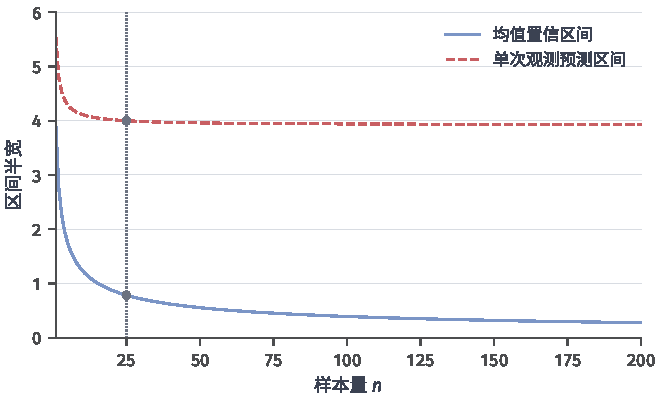
\includegraphics[width=\linewidth]{figures/01-mathematical-preliminaries/04-random-variables-distributions-and-causality/matplotlib/statistics-mean-prediction-width/figure.pdf}
  \caption{已知\(\sigma=2\)的独立高斯位置模型中，两类区间半宽随样本量变化（解析式教学图）。使用四舍五入分位数\(1.96\)，蓝实线为\(1.96\sigma/\sqrt n\)，红虚线为\(1.96\sigma\sqrt{1+1/n}\)。灰竖线标出例~\ref{ex:statistics-running-sensor-calibration}的\(n=25\)，没有对任何实测数据重复抽样。}
  \label{fig:statistics-mean-prediction-width}
\end{figure}

\begin{table}[htbp]
  \centering
  \begin{tabular}{p{0.16\linewidth}p{0.29\linewidth}p{0.43\linewidth}}
    \toprule
    类型 & 覆盖对象 & 概率来源与必要条件\\
    \midrule
    置信区间 & 固定总体参数 & 同一抽样制度下重复构造区间的覆盖率\\
    可信区间 & 给定数据的参数后验 & 指定先验与似然形成的后验概率；不自动具有频率覆盖\\
    预测区间 & 尚未观测的随机结果 & 训练样本与未来观测的联合分布；须包含新观测波动\\
    \bottomrule
  \end{tabular}
  \caption{三类区间的覆盖对象与概率来源。区间形式相似时，仍须从所覆盖的对象解释结论。}
  \label{tab:statistics-interval-objects}
\end{table}

方差未知时，用
\[
  S^2=\frac1{n-1}\sum_{i=1}^n(Y_i-\overline Y)^2
\]
估计\(\sigma^2\)。在引理~\ref{lem:statistics-gaussian-mean-residual}的高斯独立样本条件下，
\[
  \frac{\overline Y-\theta}{S/\sqrt n}\sim t_{n-1},
\]
所以把高斯分位数换成\(t\)分位数可得到精确置信区间。这里的精确性依赖高斯性；
一般分布下它通常只是渐近近似。样本很小且分布偏斜、重尾时，机械使用该区间可能同时
破坏中心和尾部覆盖。

双侧区间与双侧检验在相同模型、显著性水平和统计量下互为反演：若
\(\theta_0\)不在\(1-\alpha\)置信区间内，就拒绝\(H_0:\theta=\theta_0\)。
这种对应关系要求两者使用相同标准误与尾部规则。选择后区间、单侧检验或离散检验中，
不能只凭表面上的阈值照搬这一关系。
% Baseline T:1171-1228
复杂估计量的抽样分布难以解析计算时，可以让经验数据模拟重复抽样。
\term{Bootstrap}从经验分布
\(\widehat P_n=n^{-1}\sum_i\Delta_{Y_i}\)有放回抽取\(n\)个观测，并重新计算
\(\widehat\tau^\ast\)。条件于原样本的
\(\widehat\tau^\ast-\widehat\tau\)近似
\(\widehat\tau-\tau(P)\)的抽样波动。简单百分位区间取Bootstrap估计值的经验分位数，
但对不光滑统计量、边界参数、极端尾部分位数或重尾小样本，近似可能很差。

对独立同分布、方差\(0<\sigma^2<\infty\)的样本均值，这个近似有清楚的缩放口径。
若\(\overline Y^\ast\)由经验分布条件重抽样，则下述条件分布依概率弱收敛：
\[
  \mathcal L\!\left(
    \sqrt n(\overline Y^\ast-\overline Y)\mid\bm Y
  \right)
  \Longrightarrow\mathcal N(0,\sigma^2),
\]
与\(\sqrt n(\overline Y-\mu)\)的极限相同。这里条件分布随原样本而变，本身是随机对象。
具体地，用\(\mathbb E_\ast\)表示给定原数据后的重抽样期望，“依概率弱收敛”指
对每个有界Lipschitz函数\(f\)，
\[
 \mathbb E_\ast f\bigl(\sqrt n(\overline Y^\ast-\overline Y)\bigr)
 \xrightarrow{\mathbb P}\mathbb E f(Z),\qquad Z\sim\mathcal N(0,\sigma^2).
\]
外层的依概率收敛针对原数据的抽样随机性。

此处需要的中心极限定理允许抽样规律随\(n\)改变。
把随机变量逐行排列，第\(n\)行有\(n\)项\(X_{n,1},\ldots,X_{n,n}\)，
这样的排列称为三角阵列（triangular array）。
若每行内的变量独立、中心化，满足
\[
 \sum_{i=1}^n\mathbb E X_{n,i}^2\longrightarrow\sigma^2>0,\qquad
 \sum_{i=1}^n\mathbb E\!\left[
 X_{n,i}^2\mathbb I\{|X_{n,i}|>\varepsilon\}\right]\longrightarrow0
\]
对每个\(\varepsilon>0\)成立，则行和趋于\(\mathcal N(0,\sigma^2)\)。
第二项称为Lindeberg条件，排除了由少数单项主导总波动的情况。
这是所用的独立三角阵列中心极限定理；不要求不同行之间独立，完整证明见概率论教材\scite{math-kallenberg2021probability}

对给定原数据的重抽样取\(X_{n,i}=(Y_i^\ast-\overline Y)/\sqrt n\)。
行和就是所研究的均值波动；条件均值为零，条件方差和是经验方差。
经验均值等于\(\overline Y\)，经验方差
依概率趋于\(\sigma^2\)，但方差收敛本身还不足以保证条件中心极限定理。有限二阶矩还使
每个\(\varepsilon>0\)对应的条件Lindeberg尾项满足
\[
  \frac1n\sum_{i=1}^n(Y_i-\overline Y)^2
  \mathbb I\{|Y_i-\overline Y|>\varepsilon\sqrt n\}
  \xrightarrow{\mathbb P}0.
\]
这个经验尾项恰好是上述阵列在条件分布下的Lindeberg和。
其收敛可直接由有限二阶矩核对。以趋于一的概率
\(|\overline Y-\mu|\leq\varepsilon\sqrt n/2\)；在此事件上，
若\(|Y_i-\overline Y|>\varepsilon\sqrt n\)，则
\(|Y_i-\mu|>\varepsilon\sqrt n/2\)。又有
\[
 (Y_i-\overline Y)^2\leq2(Y_i-\mu)^2+2(\overline Y-\mu)^2.
\]
因此经验尾项被原中心平方尾的两倍经验平均加\(2(\overline Y-\mu)^2\)控制。
第一项的期望随截断阈值增大而趋零，由Markov不等式依概率趋零；第二项由大数定律趋零。

为把随机条件量接到确定阵列定理，可从任意原数据子列中再抽出一条子子列，
使经验方差和所有正有理\(\varepsilon\)的尾项同时几乎必然收敛；
这是引理~\ref{lem:rv-probability-subsequence}的可数对角应用。
尾项关于阈值单调，故该共同满测集上所有正阈值的条件都成立。
逐条固定这样的原数据实现，应用阵列定理便得到条件弱收敛；
再用同一子列判据返回上述测试函数积分的依概率结论。
该结论针对中心化、缩放后的条件分布；它本身不自动证明任意百分位
区间具有高阶准确性。

例~\ref{ex:statistics-running-sensor-calibration}中的经验分布均值为\(10.4\)，经验
方差按分母\(n\)计算恰为\(4\)。因此单次Bootstrap抽样值满足
\[
  \mathbb{E}_\ast[Y^\ast]=10.4,\qquad
  \operatorname{Var}_\ast(Y^\ast)=4,
\]
而二十五次有放回抽样的均值满足
\[
  \operatorname{SE}_\ast(\overline Y^\ast)
  =
  \sqrt{\frac4{25}}=0.4.
\]
若中心化并按标准误标准化后的条件Bootstrap分布可由标准正态分布近似，则正态
Bootstrap区间为
\(10.4\pm1.96\times0.4=[9.62,11.18]\)，与已知方差高斯区间在这个构造例中重合。
重合来自经验方差刚好等于已知噪声方差以及均值的光滑性，不是Bootstrap总会复制参数
区间的保证。

更一般的统计量可以用线性化研究，但须分别控制原抽样与重抽样的余项。即使已经证明
\[
  \widehat\tau-\tau(P)
  =
  \frac1n\sum_{i=1}^n\operatorname{IF}(Y_i;T,P)
  +o_{\mathbb{P}}(n^{-1/2}),
\]
也还需证明条件重抽样展开，例如对某个数据依赖的中心化函数\(\phi_n\)，
\[
 \widehat\tau^\ast-\widehat\tau
 =\frac1n\sum_{i=1}^n\phi_n(Y_i^\ast)+r_n^\ast,\qquad
 \mathbb E_\ast\phi_n(Y_i^\ast)=0.
\]
所需余项条件是：对每个\(\varepsilon>0\)，
\(\mathbb P_\ast(\sqrt n|r_n^\ast|>\varepsilon)\xrightarrow{\mathbb P}0\)；
这就是这里的条件\(o_{\mathbb P_\ast}(n^{-1/2})\)。
若经验影响函数\(\phi_n\)还满足条件中心极限定理，且极限方差与原影响函数一致，
两边缩放后的分布才趋于同一极限。适当的统计泛函光滑性可以帮助建立这些条件，
不能只把原展开中的\(P\)换成\(\widehat P_n\)便认定已证明Bootstrap有效\scite{vanderVaart1998asymptotic}

一个短反例说明为何必须单独检查重抽样。连续有限方差分布下，取
\[
 \widehat\tau_n=\overline Y+n^{-1/2}
 \mathbb I\{\text{样本中有重复值}\}.
\]
原样本几乎必然没有重复值，所以它具有与均值完全相同的原抽样展开。
但从\(n\)个不同观测有放回抽\(n\)次，全不重复的条件概率为
\(n!/n^n\leq\exp(-(n-1)/2)\)，趋于零；不等式来自
\(\log(1-j/n)\leq-j/n\)的逐项求和。
于是\(\sqrt n(\widehat\tau_n^\ast-\widehat\tau_n)\)额外平移约\(1\)，
没有逼近原统计量的中心化极限。
样本最大值之类统计量
没有这种常规线性展开：经验分布不会生成比当前最大值更大的观测，简单Bootstrap便可能
错误描述尾部。
% Baseline T:1247-1249
重采样单位必须跟独立单位一致。配对实验对整对数据重采样；多个记录属于同一用户时对
用户群组重采样；时间相关数据使用保留局部依赖的块Bootstrap。逐条重采样会把共享噪声
误当作独立波动，通常低估标准误。
% Baseline S:642-649
\begin{definition}[置信序列]
  \label{def:stoch-confidence-sequence}
  对参数为\(\theta\)时的数据分布\(\mathbb P_\theta\)，数据依赖集合\((C_t)_{t\geq1}\)若在时刻\(t\)由\(\mathcal F_t\)确定，且对每个允许的\(\theta\)满足
  \[ \mathbb P_\theta(\theta\in C_t\text{ 对所有 }t\geq1)\geq1-\delta, \]
  则称为覆盖水平\(1-\delta\)的\term{置信序列}（confidence sequence），其中\(0<\delta<1\)。
\end{definition}
它在同一个高概率事件上覆盖所有时刻，因而允许根据当前数据决定何时查看或停止。固定$n$的置信区间只承诺
预先指定时刻的覆盖；反复查看直到区间排除某个值，会改变错误概率。
一个可直接计算的标量构造来自Hoeffding界。若\(X_i\in[0,1]\)独立同分布，均值为
\(\mu\)，给第\(n\)次查看分配错误预算
\(\delta_n=\delta/[n(n+1)]\)，则\(\sum_{n\geq1}\delta_n=\delta\)。定义
\[
C_n=\left[\overline X_n-
\sqrt{\frac{\log(2n(n+1)/\delta)}{2n}},
\ \overline X_n+
\sqrt{\frac{\log(2n(n+1)/\delta)}{2n}}\right]\cap[0,1].
\]
对全部时刻的坏事件取并集，即得
\(\mathbb P(\forall n,\mu\in C_n)\geq1-\delta\)。
取\(\delta=0.05,n=100\)，半宽约为\(0.254\)；固定时刻Hoeffding区间半宽约为
\(0.136\)。同时保证付出了更宽范围，这个简单预算构造也不是最紧的边界。条件均值恒为
\(\mu\)且条件范围仍为\([0,1]\)时，条件Hoeffding论证给出同样控制；任意相关观测则不能直接使用。
预先固定有限个候选时，可再将\(\delta\)分给各候选以保证选择后的覆盖。无限搜索或用同一数据重新设计目标，需要额外统一控制或独立评价数据。

对于可预测的向量设计，下面回用第~\ref{sec:rv-anytime}节的自归一化界，把累计噪声转成参数置信椭球。
% Baseline S:816-924
取$\bm{V}_0=\lambda\bm{I}$，$\lambda>0$，并定义岭回归估计
\begin{equation}
  \widehat{\bm{\theta}}_t
  =\bm{V}_t^{-1}\sum_{s=1}^{t}\bm{x}_s y_s.
  \label{eq:stoch-ridge-estimator}
\end{equation}
由式~\eqref{eq:stoch-adaptive-linear-observation}，
\[
  \bm{V}_t
  (\widehat{\bm{\theta}}_t-\bm{\theta}^{\star})
  =
  \bm{S}_t-\lambda\bm{\theta}^{\star}.
  \]
若还知道$\lVert\bm{\theta}^{\star}\rVert_2\leq B$，三角不等式给出
\begin{align}
  \lVert
    \widehat{\bm{\theta}}_t-\bm{\theta}^{\star}
  \rVert_{\bm{V}_t}
  &\leq
  \lVert\bm{S}_t\rVert_{\bm{V}_t^{-1}}
  +
  \lambda
  \lVert\bm{\theta}^{\star}\rVert_{\bm{V}_t^{-1}}
  \notag\\
  &\leq
  R\sqrt{
    2\log\left(
      \frac{\det(\bm{V}_t)^{1/2}}
           {\lambda^{d/2}\delta}
    \right)
  }
  +\sqrt{\lambda}B
  =:\beta_t(\delta).
  \label{eq:stoch-adaptive-confidence-ellipsoid}
\end{align}
第二个不等式使用$\bm{V}_t\succeq\lambda\bm{I}$。因此
\[
  \mathcal{C}_t(\delta)
  =
  \left\{
    \bm{\theta}:
    \lVert\bm{\theta}-\widehat{\bm{\theta}}_t
    \rVert_{\bm{V}_t}
    \leq\beta_t(\delta)
  \right\}
\]
在同一个概率至少为$1-\delta$的事件上，对所有$t$都包含真实参数。这是置信椭球而不是
欧氏球：观测充分的方向较窄，信息不足的方向较宽。

\begin{example}[二维自适应查询]
  \label{ex:stoch-two-dimensional-adaptive-design}
  设$d=2$、$\lambda=1$，每次只能在
  $\bm{e}_1=(1,0)^\top$与$\bm{e}_2=(0,1)^\top$中选择一个观测方向。算法可以在第
  $t$步比较当前椭球在两个方向上的宽度，并选择较宽的方向；这个选择只依赖过去，因而
  $\bm{x}_t$可预测。

  若前四次选择中$\bm{e}_1$出现三次、$\bm{e}_2$出现一次，则
  \[
    \bm{V}_4
    =
    \begin{pmatrix}
      4&0\\
      0&2
    \end{pmatrix},
    \qquad
    \det(\bm{V}_4)=8.
  \]
  对任意方向$\bm{x}$，椭球给出的预测误差满足
  \[
    |\langle
      \bm{x},
      \widehat{\bm{\theta}}_4-\bm{\theta}^{\star}
    \rangle|
    \leq
    \beta_4(\delta)
    \lVert\bm{x}\rVert_{\bm{V}_4^{-1}}.
  \]
  因而两个坐标方向的半宽分别与$1/2$和$1/\sqrt2$成比例。第一个方向访问更多，区间
  更窄；下一次转向第二个方向是由已有信息决定的自适应设计。定理仍然适用，因为它在每次
  新噪声产生之前固定当前方向，并在一个事件上同时控制全部时刻。
\end{example}

图~\ref{fig:stochastic-design-ellipsoids}还比较了相同四次预算在两个方向各访问两次的情形：此时\(\bm V_4=\operatorname{diag}(3,3)\)。均衡访问扩大第一个方向的几何半宽，却缩小第二个方向的半宽；因此设计会改变误差的方向分配，不能只比较一个总访问数。图中把两条二次型的右侧统一设为\(1\)，仅比较几何；真正的置信椭球还要分别乘上各自的\(\beta_4(\delta)\)，其行列式项也会改变。

\begin{figure}[htbp]
  \centering
  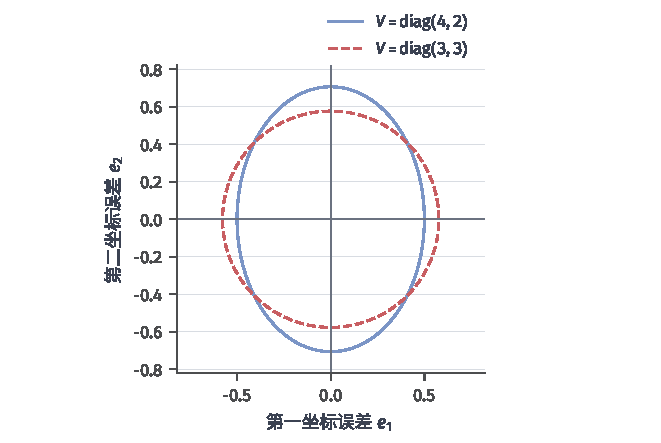
\includegraphics[width=\linewidth]{figures/01-mathematical-preliminaries/04-random-variables-distributions-and-causality/matplotlib/stochastic-design-ellipsoids/figure.pdf}
  \caption{二维设计的归一化误差几何（解析式教学图）。蓝实线为\(\bm e^\top\operatorname{diag}(4,2)\bm e=1\)，红虚线为\(\bm e^\top\operatorname{diag}(3,3)\bm e=1\)。它们不是已经具有相同覆盖概率的数值置信区间；真实置信半径由式~\eqref{eq:stoch-adaptive-confidence-ellipsoid}另行确定。}
  \label{fig:stochastic-design-ellipsoids}
\end{figure}

这个例子也说明为什么不能把独立样本界中的$n$换成某个动作的访问次数。参数误差是向量，
不同特征方向可能相关；置信宽度由$\bm{x}^{\top}\bm{V}_t^{-1}\bm{x}$决定，而不是只由
某个坐标被访问多少次决定。行列式项又要为算法可能探索的全部方向支付复杂度。

\par\medskip\noindent\textbf{可预测设计与数据依赖的边界}\quad
自归一化界允许$\bm{x}_t$依赖$\mathcal{F}_{t-1}$，不允许它依赖当前$\eta_t$后再伪装成
预先选择。若传感器先看到当前噪声再决定是否记录，$\bm{x}_t\eta_t$的条件平均可能不再为
零，指数超鞅的第一步就会失败。类似地，模型失配使
$\mathbb{E}[y_t\mid\mathcal{F}_{t-1},\bm{x}_t]$不等于
$\langle\bm{x}_t,\bm{\theta}^{\star}\rangle$时，椭球会同时包含系统偏差与随机误差，
不能继续解释为围绕同一个真实参数的置信集合。

条件次高斯性也不是有限方差的同义词。重尾噪声可能需要截断、稳健均值或只使用有限矩的
其他序贯工具；直接套用式~\eqref{eq:stoch-vector-self-normalized-bound}会低估尾部。
$\lambda$保证初期矩阵可逆并编码参数范数先验，但过大的$\lambda$会增加
$\sqrt{\lambda}B$偏差项。置信椭球控制统计误差，不保证选择策略会访问所有对任务重要的
方向；探索是否充分仍要由设计规则与任务目标另行证明。

\subsubsection{假设检验与错误控制}
\label{sec:statistics-testing-errors}
\label{sec:statistics-selection-multiplicity}
% Baseline T:1012-1164
区间描述目标的可能范围，\term{假设检验}（hypothesis testing）则检查数据与一个
命题是否相容。
\begin{definition}[随机化检验函数]
  \label{def:statistics-randomized-test-function}
  若单个观测的可测空间为\(\mathcal{Y}\)，则
  \term{随机化检验函数}（randomized test function）是可测映射
  \[
    \varphi:\mathcal{Y}^n\to[0,1].
  \]
  观察到\(\bm{Y}=\bm{y}\)后，检验以概率\(\varphi(\bm{y})\)拒绝原假设。等价地，可另取
  独立的\(U\sim\operatorname{Unif}(0,1)\)，并在
  \(U\leq\varphi(\bm{y})\)时拒绝。只取\(0,1\)值的检验是非随机化特例，其拒绝域为
  \(R=\{\bm{y}:\varphi(\bm{y})=1\}\)。
\end{definition}

原假设\(H_0\)指定被控制误报的情形。检验的大小与参数\(\theta\)下的功效分别为
\[
  \sup_{\theta\in H_0}\mathbb{E}_\theta[\varphi(\bm Y)],
  \qquad
  \mathbb{E}_\theta[\varphi(\bm Y)].
\]
水平为\(\alpha\)要求
\[
  \sup_{\theta\in H_0}
  \mathbb{E}_\theta[\varphi(\bm Y)]
  \leq\alpha.
\]
在\(H_0\)为真时拒绝是第一类错误；在备择\(H_1\)为真时不拒绝是第二类错误。
对非随机化检验，这些期望分别退化为拒绝域概率。效应量描述差异有多大，样本量则影响
能否把该差异从噪声中区分出来。

\term{\(p\)值}（\(p\)-value）是在原假设下，得到至少与当前统计量同样极端结果的
概率。
\begin{definition}[有效p值]
  \label{def:statistics-valid-p-value}
  一个取值于\([0,1]\)的可测统计量\(p(\bm Y)\)是复合原假设\(H_0\)下的有效\(p\)值，若对每个
\(u\in[0,1]\)都有
\[
  \sup_{\theta\in H_0}\mathbb{P}_\theta\{p(\bm Y)\leq u\}\leq u.
\]
\end{definition}
这项零假设下的超均匀性质才保证按阈值\(\alpha\)拒绝时控制第一类错误。观察到的
\(p\)值不是原假设为真的概率，也不是效应量。仍取已知\(\sigma\)的高斯位置模型，
检验\(H_0:\theta=0\)时
\[
  Z=\frac{\sqrt n\,\overline Y}{\sigma},\qquad
  p=2\{1-\Phi(|Z|)\}.
\]
若\(\theta=\delta\)，双侧检验功效为
\[
  \mathbb{P}_\delta(|Z|>z_{1-\alpha/2})
  =
  1-\Phi\left(z_{1-\alpha/2}-\frac{\sqrt n\delta}{\sigma}\right)
  +\Phi\left(-z_{1-\alpha/2}-\frac{\sqrt n\delta}{\sigma}\right).
\]
小样本下“不显著”可能只表示功效不足。相同效应量在更大\(n\)下会得到更小的
\(p\)值。

检验族还可反演为置信集合。对每个候选值\(\theta_0\)，设
\(\varphi_{\theta_0}(\bm Y)\in\{0,1\}\)是水平不超过\(\alpha\)的检验，并定义
\[
  C(\bm Y)=\{\theta_0:\varphi_{\theta_0}(\bm Y)=0\}.
\]
当真实值为\(\theta\)时，
\[
  \mathbb{P}_\theta\{\theta\notin C(\bm Y)\}
  =\mathbb{P}_\theta\{\varphi_\theta(\bm Y)=1\}\leq\alpha,
\]
所以\(C\)具有至少\(1-\alpha\)覆盖率。这里必须对同一模型、同一尾部规则和同一
标准误反演；选择后换检验或只挑有利方向会破坏证明。

\begin{example}[同一效应量下的证据与功效]
\label{ex:statistics-evidence-power-same-effect}
设噪声标准差已知为\(\sigma=2\)，观测均值为\(\overline y=1\)，检验
\(H_0:\theta=0\)。当\(n=4\)时，\(Z=1\)，双侧\(p\)值约为\(0.317\)；
当\(n=100\)时，\(Z=5\)，双侧\(p\)值小于\(10^{-6}\)。两次实验报告的标准化
效应\(\overline y/\sigma=0.5\)相同，证据强度却因标准误不同而变化。

若真实值确为\(\delta=1\)，显著性水平为\(0.05\)，则\(n=4\)时双侧检验功效约为
\[
  1-\Phi(1.96-1)+\Phi(-1.96-1)\approx0.17.
\]
此时未拒绝原假设并不支持“差异为零”。若实际问题把绝对差异不超过\(0.2\)视为等效，
还需要针对\(\Delta=0.2\)设计等效检验；当前样本对这个更严格目标几乎没有辨识力。
\end{example}

\par\medskip\noindent\textbf{似然比排序与Neyman–Pearson引理}\quad
下面的经典引理给出两个简单假设之间的最强检验\scite{math-lehmann2005testing}
\begin{theorem}[Neyman--Pearson引理]
\label{thm:statistics-neyman-pearson}
对两个完全指定的简单假设\(H_0:P=P_0\)与\(H_1:P=P_1\)，设
\(P_1\ll P_0\)，似然比为\(\Lambda=\mathrm dP_1/\mathrm dP_0\)。在所有大小
不超过\(\alpha\)的检验中，拒绝大似然比并在边界适当随机化的检验具有最大功效。
\end{theorem}

\begin{proof}
取常数\(c\)与边界随机化概率，使检验\(\varphi^\star\)满足
\(\mathbb{E}_0[\varphi^\star]=\alpha\)，并在\(\Lambda>c\)时拒绝、在
\(\Lambda<c\)时接受。对任意\(\mathbb{E}_0[\varphi]\leq\alpha\)的检验，
\[
  (\varphi^\star-\varphi)(\Lambda-c)\geq0
\]
逐点成立，因为\(\varphi^\star\)在\(\Lambda>c\)处取最大允许值，在
\(\Lambda<c\)处取最小允许值。对\(P_0\)积分得到
\[
  \mathbb{E}_1[\varphi^\star-\varphi]
  \geq c\,\mathbb{E}_0[\varphi^\star-\varphi]\geq0.
\]
所以\(\varphi^\star\)的备择拒绝概率不小于任何同大小检验。
\end{proof}

这个结论只直接覆盖两个简单假设。复合假设需要处理未知参数，不一定存在一致最强检验。
在隐私攻击审计中，\(P_0\)与\(P_1\)可分别表示目标记录不在与在训练集时的输出分布；
似然比给出理想攻击排序，但实际审计还要估计这两个分布并计入选择偏差。

\par\medskip\noindent\textbf{列联表、渐近检验与不同命题}\quad
两个分类变量的列联表中，原假设为独立时，期望格数是
\[
  E_{r,c}=\frac{N_{r,\cdot}N_{\cdot,c}}{N},\qquad
  X^2=\sum_{r,c}\frac{(N_{r,c}-E_{r,c})^2}{E_{r,c}}.
\]
在独立抽样、固定维数且期望格数不过小时，
\(X^2\)近似服从自由度\((R-1)(C-1)\)的卡方分布。稀疏格数会破坏近似，可合并有
科学意义的类别或使用精确、置换方法。条件独立检验还要控制第三个变量；把样本简单切成
大量小层会带来新的稀疏性，不能由普通卡方检验自动解决。

差异检验把“无差异”放在原假设中。等效性检验先给出有实际含义的可接受差异界
\(\Delta>0\)。记\(\delta=\theta_A-\theta_B\)，两个单侧检验（two one-sided
tests, TOST）把不等效原假设写成两个集合的并：
\[
  H_0=H_{0,L}\cup H_{0,U},
  \qquad
  H_{0,L}:\delta\leq-\Delta,
  \qquad
  H_{0,U}:\delta\geq\Delta.
\]
对应备择为\(-\Delta<\delta<\Delta\)。TOST只有在水平\(\alpha\)的下侧检验拒绝
\(H_{0,L}\)，并且水平\(\alpha\)的上侧检验也拒绝\(H_{0,U}\)时，才拒绝总体原假设。
例如，若\(\widehat\delta\)的标准误为\(s\)，且标准化统计量服从相应正态近似，
拒绝条件为
\begin{equation}
  \frac{\widehat\delta+\Delta}{s}>z_{1-\alpha}
  \quad\text{且}\quad
  \frac{\widehat\delta-\Delta}{s}<z_{\alpha}.
  \label{eq:statistics-tost-rejection}
\end{equation}
这等价于把双侧\(1-2\alpha\)置信区间完整放入
\((-\Delta,\Delta)\)。总体第一类错误并非\(2\alpha\)：只要
\(\delta\in H_0\)，至少有一个单侧原假设为真，而总体拒绝事件包含在拒绝这个真原假设
的事件中，所以其概率至多为\(\alpha\)。非劣效检验只排除一个方向，例如
\(H_0:\delta\leq-\Delta\)。未拒绝差异检验的零假设不等于证明等效。
% Baseline T:1232-1245
\term{置换检验}（permutation test）近似的不是估计量抽样分布，而是零假设下标签可
交换时的随机化分布。两组观测在“处理标签不影响联合分布”的原假设下，可反复打乱标签
并重算组间差异。若分配机制只允许在区组内交换，就必须在区组内置换；任意全局打乱会
制造实验中不可能出现的分配。

若允许的置换集合有\(M\)个元素，并把观测统计量与全部置换统计量一起排序，则交换
对称性使真实排列的秩在这些位置上均匀；存在并列时使用
\[
  p_{\mathrm{perm}}
  =\frac{\#\{\text{置换统计量不小于观测值}\}}{M}
\]
得到超均匀而可能保守的\(p\)值。若只随机抽取\(B\)个置换，常用
\((1+\#\{\text{抽样置换不小于观测值}\})/(B+1)\)保留有限模拟下的保守性。
仅有两组均值相等并不保证整批标签可交换；交换性必须来自更强的零假设或随机分配设计。
% Baseline T:1256-1293
单个检验的第一类错误为\(\alpha\)，不代表同时尝试许多候选后仍只有
\(\alpha\)的误报概率。若\(m\)个原假设都为真，联合界给出
\[
  \mathbb{P}(\text{至少一次误拒绝})
  \leq\sum_{j=1}^m\mathbb{P}(\text{拒绝 }H_j)
  \leq m\alpha.
\]
Bonferroni方法把每项阈值设为\(\alpha/m\)，从而控制
\term{族错误率}（family-wise error rate, FWER）。它不要求检验独立，但候选很多时
可能保守。

Holm方法把\(p\)值从小到大排序，并依次将
\(p_{(j)}\)与\(\alpha/(m-j+1)\)比较，遇到第一个未拒绝项即停止。若第一个被错误
拒绝的真原假设位于位置\(j\)，设真原假设总数为\(m_0\)，则前\(j-1\)项均为假
原假设，所以\(m-j+1\geq m_0\)。该真原假设的\(p\)值因而不超过
\(\alpha/(m-j+1)\leq\alpha/m_0\)。对全部\(m_0\)个真原假设应用联合界，便把
发生任一错误拒绝的概率控制在\(\alpha\)以内。它与Bonferroni一样不要求独立，但利用
了逐步比较。

当目标是控制所有拒绝中错误发现的期望比例时，可使用
\term{错误发现率}（false discovery rate, FDR）。设\(R\)为拒绝的总数、\(V\)为其中
被错误拒绝的真原假设数，则
\[
  \operatorname{FDR}=\mathbb E\left[\frac{V}{\max(R,1)}\right].
\]
当\(R=0\)时，错误发现比例约定为零；这是随机比例的期望，不是
\(\mathbb EV/\mathbb ER\)。Benjamini--Hochberg过程将
\(p\)值排序为\(p_{(1)}\leq\cdots\leq p_{(m)}\)，找最大
\[
  k=\max\left\{j:p_{(j)}\leq\frac{j}{m}q\right\},
\]
并拒绝前\(k\)项；若集合为空，则取\(k=0\)，不拒绝任何假设。若全部\(p\)值相互
独立，且每个真原假设下的\(p\)值满足
\(\mathbb P(p_j\leq u)\leq u\)（\(0\leq u\leq1\)），该过程控制FDR不超过目标
\(q\in(0,1)\)\scite{statistics-benjamini-hochberg1995}扩展到依赖检验需要更精确的联合分布条件，不能仅凭两两正相关或任意
依赖就沿用这项保证。

从多个模型中挑选测试误差最小者，再把该最小值当成固定模型的无偏评估，会系统性偏乐观。
% Baseline T:1330-1343
持续查看同一数据也构成选择。固定时刻满足
\(\mathbb{P}(p_t\leq\alpha)\leq\alpha\)并不推出
\(\mathbb{P}(\exists t:p_t\leq\alpha)\leq\alpha\)。预先规定查看次数可分配
\(\alpha\)预算；更灵活的停止规则需要序贯检验、置信序列或对整个证据过程的控制。
停止规则属于推断程序的一部分，不能在看到结果后删去。

一种单次证据是\(e\)值（e-value）：非负统计量\(E\)若在每个零假设分布\(P\)下
满足\(\mathbb E_PE\leq1\)，就称为有效\(e\)值。由Markov不等式，
\(P(E\geq1/\alpha)\leq\alpha\)，所以大值可以用来拒绝零假设。
但逐个固定时刻的\(E_t\)都是有效\(e\)值，仍不足以保证可以任意停止；
下文用非负超鞅给出一种能同时控制所有时刻的证据过程。

定义~\ref{def:stoch-confidence-sequence}的\term{置信序列}（confidence sequence）把所有时刻的覆盖放在同一个高概率事件中。这比每个固定时刻各自覆盖更强，因为允许依据当前数据决定何时停止查看。
若\((E_t)\)在原假设下是从\(E_0=1\)开始的非负超鞅，则Ville不等式给出
\[
  \mathbb{P}_0\left\{\sup_{t\geq0}E_t\geq\frac1\alpha\right\}\leq\alpha.
\]
因此可以在任意由过去信息决定的停止时刻按阈值查看\(E_t\)，而不增加这项越界概率。
这不表示停止后的点估计无偏，也不表示同时尝试多个证据过程无需额外控制；覆盖、估计
偏差和模型选择证据仍是不同问题。

\subsection{模型比较与观测设计}
\label{sec:stats-model-comparison-data-acquisition}
已有观测可以用来选择候选规律，剩余预算则允许选择新的观测。两类选择的目标不同：模型证据、未来风险和信息价值不能直接共用一个解释。

\subsubsection{给定观测下的模型比较}
\label{sec:statistics-model-evidence}
% Baseline T:1595-1754
上一组工具评价预测分布；多个模型竞争时，还需先决定比较的是训练拟合、未来预测还是模型证据。
边缘似然对参数积分，Laplace近似用局部曲率近似这项积分。
信息准则的惩罚形式虽可能相似，比较目标和渐近条件却不同。

\par\medskip\noindent\textbf{预测、似然与边缘似然}\quad
模型选择准则并非都在回答同一问题。独立测试误差比较未来预测；训练似然衡量已观测数据
在拟合参数下的密度；边缘似然
\[
  p(\bm y\mid M)
  =\int p(\bm y\mid\vartheta,M)\pi(\vartheta\mid M)\,\mathrm d\vartheta
\]
对参数不确定性积分；编码长度则把模型和数据的描述代价相加。一个模型可能训练似然高，
却因复杂度、先验体积或泛化误差而不被其他准则选择。

\begin{definition}[Bayes因子]
  \label{def:statistics-bayes-factor}
两个模型\(M_1,M_0\)的\term{Bayes因子}（Bayes factor）是
\[
  \operatorname{BF}_{1,0}
  =\frac{p(\bm y\mid M_1)}{p(\bm y\mid M_0)}.
\]
这里两个边缘似然都由概率先验得到；所比较的数据处，分母严格为正且有限，分子有限且可为零。
\end{definition}
Bayes因子更新的是模型间先验赔率，
不是与先验无关的“模型为真概率”。在高斯位置模型中，若
\(\theta\sim\mathcal N(0,A^2)\)，则
\(\overline Y\sim\mathcal N(0,A^2+\sigma^2/n)\)。保持似然峰值不变而增大\(A\)
会把先验质量摊到更宽区域；对固定\(\overline y\)，当\(A\to\infty\)时该边缘密度
趋于零。这正是模型证据依赖参数先验尺度的一个可复核例子。

\par\medskip\noindent\textbf{Laplace近似与BIC}\quad
\begin{theorem}[固定维Laplace局部积分近似]
\label{thm:statistics-laplace-approximation}
设\(\Theta\subseteq\mathbb{R}^d\)为可测集，
\(\widehat{\bm\vartheta}\in\operatorname{int}(\Theta)\)。函数
\(h:\Theta\to\mathbb{R}\)可测，并在
\(\widehat{\bm\vartheta}\)的某个邻域内二阶连续可微；该点是\(h\)在\(\Theta\)上的
唯一全局最大点，且
\(\bm H=-\nabla^2h(\widehat{\bm\vartheta})\)正定。函数
\(g:\Theta\to[0,\infty)\)局部可积，在该点的某个邻域内连续，并满足
\(g(\widehat{\bm\vartheta})>0\)。

进一步假设存在\(\delta,\eta>0\)和\(n_0\geq1\)，使
\(\overline{B_\delta(\widehat{\bm\vartheta})}\subseteq\Theta\)，\(h,g\)在该闭球
所在的邻域内分别满足上述光滑性与连续性，并且
\[
  \sup_{\bm\vartheta\in
    \Theta\setminus B_\delta(\widehat{\bm\vartheta})}
  h(\bm\vartheta)
  \leq h(\widehat{\bm\vartheta})-\eta,
  \qquad
  \int_\Theta
  \exp\!\left\{n_0\bigl[h(\bm\vartheta)
    -h(\widehat{\bm\vartheta})\bigr]\right\}
  g(\bm\vartheta)\,\mathrm d\bm\vartheta<\infty.
\]
则当\(n\to\infty\)时，
\[
  \int_\Theta \exp\{n h(\bm\vartheta)\}g(\bm\vartheta)\,
  \mathrm d\bm\vartheta
  =
  \exp\{nh(\widehat{\bm\vartheta})\}
  g(\widehat{\bm\vartheta})
  \left(\frac{2\pi}{n}\right)^{d/2}
  |\bm H|^{-1/2}\{1+o(1)\}.
\]
\end{theorem}

\begin{proof}
正定性与二阶连续性保证：必要时缩小\(\delta\)，存在\(c>0\)，使闭球内有
\[
  h(\bm\vartheta)-h(\widehat{\bm\vartheta})
  \leq-c\lVert\bm\vartheta-\widehat{\bm\vartheta}\rVert_2^2.
\]
缩小闭球后，原闭球中剩余的紧致环带由唯一最大性给出严格间隔；把它与原来的尾部间隔
合并，仍可取某个\(\eta>0\)满足定理中的一致上界。另一方面，在最大点附近作多元
Taylor展开：
\[
  h(\bm\vartheta)
  =
  h(\widehat{\bm\vartheta})
  -\frac12(\bm\vartheta-\widehat{\bm\vartheta})^\top
  \bm H(\bm\vartheta-\widehat{\bm\vartheta})
  +o(\lVert\bm\vartheta-\widehat{\bm\vartheta}\rVert_2^2).
\]
令
\(\bm u=\sqrt n\,\bm H^{1/2}
(\bm\vartheta-\widehat{\bm\vartheta})\)，则逆变换的Jacobian行列式绝对值为
\(n^{-d/2}|\bm H|^{-1/2}\)，即
\(\mathrm d\bm\vartheta
=n^{-d/2}|\bm H|^{-1/2}\mathrm d\bm u\)。对每个固定的\(\bm u\)，
Taylor展开与\(g\)的连续性
使变换后的被积函数收敛到
\(g(\widehat{\bm\vartheta})\exp(-\lVert\bm u\rVert_2^2/2)\)。局部二次上界和
\(g\)在闭球上的有界性给出可积的高斯控制函数，因此支配收敛定理给出
\[
  \int_{B_\delta(\widehat{\bm\vartheta})}
  \exp\!\left\{n\bigl[h(\bm\vartheta)
    -h(\widehat{\bm\vartheta})\bigr]\right\}
  g(\bm\vartheta)\,\mathrm d\bm\vartheta
  =
  n^{-d/2}|\bm H|^{-1/2}
  g(\widehat{\bm\vartheta})(2\pi)^{d/2}\{1+o(1)\}.
\]
闭球外的尾项满足
\[
  \int_{\Theta\setminus B_\delta(\widehat{\bm\vartheta})}
  e^{n[h(\bm\vartheta)-h(\widehat{\bm\vartheta})]}
  g(\bm\vartheta)\,\mathrm d\bm\vartheta
  \leq
  e^{-(n-n_0)\eta}
  \int_\Theta
  e^{n_0[h(\bm\vartheta)-h(\widehat{\bm\vartheta})]}
  g(\bm\vartheta)\,\mathrm d\bm\vartheta
  =o(n^{-d/2}).
\]
局部主项与该尾项相加即得结论。
\end{proof}

上一定理描述固定函数\(h\)的基本形式。在正则独立样本模型中，实际处理的是随机函数
序列
\[
  nh_n(\bm\vartheta)=\ell_n(\bm\vartheta)
  =\sum_{i=1}^n\log p_\vartheta(y_i),\qquad
  g(\bm\vartheta)=\pi(\bm\vartheta).
\]
若极大似然估计以内点唯一最大点的形式收敛，归一化观测信息矩阵收敛到正定极限，先验
在极限点附近连续且为正，并且局部二次展开与尾部控制对该序列一致成立，则相同论证给出
\[
  \log p(\bm y\mid M)
  =
  \ell_n(\widehat{\bm\vartheta})
  -\frac d2\log n+O_{\mathbb{P}}(1).
\]
对固定的有限候选模型集合，乘以\(-2\)并只保留随\(n\)发散的项，得到常用形式
\[
  \operatorname{BIC}
  =-2\ell_n(\widehat{\bm\vartheta})+d\log n.
\]
惩罚来自后验高密度区域体积随\(n^{-d/2}\)缩小，而不是人为给参数个数加价。

\par\medskip\noindent\textbf{AIC、描述长度与比较口径}\quad
在独立、固定维且正则的最大似然设定中，常用
\[
  \operatorname{AIC}
  =-2\ell_n(\widehat{\bm\vartheta})+2d.
\]
其中\(2d\)是一阶校正拟合对预期样本外对数损失的乐观偏差，目标是预测失配；模型失配
时还要核对适用的协方差校正，不能只数参数。BIC近似特定先验下的边缘似然，常以候选中
存在真模型的正则渐近为背景。\term{最小描述长度}（minimum description length,
MDL）则先规定可解码的模型代码与给定模型后的数据代码，再最小化二者总长度；更换编码
对象或精度约定会改变有限样本准则。三者惩罚形式相似时也不能互换解释，更不能共享未经
证明的选择一致性。

混合模型的标签交换、参数位于边界、额外成分权重为零或Fisher信息奇异时，最大点可能
不唯一，局部曲率可能退化，常规Laplace展开和\(d\log n\)惩罚随之失效。此时应使用
适合奇异模型的方法、数值积分或明确的近似；近似边缘似然不能写成精确证据。

\subsubsection{给定预算下的观测设计}
\label{sec:statistics-design-information}
% Baseline T:1761-1843
推断质量不仅由分析方法决定，也由数据如何取得决定。每个对象在各处理下本会产生的结果
称为潜在结果，正式的因果目标将在第~\ref{chap:causal-inference}章定义。随机分配使
处理指派在设计上独立于这些预先固定的结果，从而把系统差异转成可量化的随机误差。
配对对照先按对象或关键协变量配对，
再在对内比较，可消除共享噪声。若配对质量差或分析时忽略配对，预期的方差收益不会自动
出现。

先看最简单的两组位置模型。若随机分配后两组分别有\(n_A,n_B\)个独立观测，均值为
\(\mu_A,\mu_B\)，方差为\(\sigma_A^2,\sigma_B^2\)，则
\[
  \widehat\Delta=\overline Y_A-\overline Y_B,\qquad
  \mathbb{E}[\widehat\Delta]=\mu_A-\mu_B,
\]
\[
  \operatorname{Var}(\widehat\Delta)
  =\frac{\sigma_A^2}{n_A}+\frac{\sigma_B^2}{n_B}.
\]
随机化建立的是处理指派与处理前对象特征之间的概率关系，并不要求两种处理下的结果
服从同一分布。上式还假设组间独立且组内方差有限；配对随机化应改为分析对内差值。
它提供的是设计下的可复核比较，潜在结果目标及从试验人群向目标总体的推广条件由
第~\ref{chap:causal-inference}章继续建立。

消融实验删除一个组件并保持其他条件不变，用来判断该组件对整体结果的增量贡献。它不能
在组件强交互时给出唯一的“独立贡献”，也不能用不同训练预算的两个系统冒充单因素比较。
基线、随机种子、停止规则和评价集都应在比较前固定。

学习曲线把训练样本量或计算量与验证性能联系起来。只报告最终点无法区分方法是数据效率
更高，还是只是使用了更多数据和算力。实验至少要区分数据预算、计算预算与评价时间预算：
收集更多标签、搜索更多配置和反复占用测试集是三种不同资源。

\par\medskip\noindent\textbf{预算下的精度与信息价值}\quad
预算分配应对应希望降低的误差。若两组单位观测成本相同且
\(n_A+n_B=N\)，最小化上面的均值差方差可得
\[
  \frac{n_A}{n_B}=\frac{\sigma_A}{\sigma_B}.
\]
这是对\(n_A\)求导或用Cauchy--Schwarz得到的Neyman分配：波动较大的组需要更多
观测。方差未知时要用先验信息或先导样本估计，估计误差也应计入设计；整数、最低组规模
和不同成本会改变解。

线性观测模型
\(\bm y=\bm X\bm\beta+\bm\varepsilon\)提供了多方向设计的接口，其中
\(\bm X\in\mathbb{R}^{n\times d}\)、\(\bm\beta,\bm a\in\mathbb{R}^d\)。
给定满列秩设计矩阵\(\bm X\)，假设
\(\mathbb{E}[\bm\varepsilon\mid\bm X]=\bm{0}\)且
\(\operatorname{Cov}(\bm\varepsilon\mid\bm X)=\sigma^2\bm I_n\)。
普通最小二乘估计量为
\[
  \widehat{\bm\beta}
  =(\bm X^\top\bm X)^{-1}\bm X^\top\bm y.
\]
它在给定\(\bm X\)时无偏，并且
\[
  \operatorname{Var}(\bm a^\top\widehat{\bm\beta}\mid\bm X)
  =\sigma^2\bm a^\top(\bm X^\top\bm X)^{-1}\bm a.
\]
因此新增观测的特征方向会改变设计矩阵，并降低某些\(\bm a\)方向的方差；它未必同样
改善其他方向、预测总体或非线性目标。最小化最坏方向、平均方向或行列式体积会得到不同
设计准则，必须先声明评价对象。

当标注预算有限时，\term{主动学习}（active learning）根据当前模型选择下一批待标注
样本。若效用\(U\)已经包含任务收益与查询成本，一个理想选择可写成最大化期望效用增量：
\[
  x^\star\in\argmax_x
  \mathbb{E}_{Y\mid x,\mathcal D}
  \left[
    U(\mathcal D\cup\{(x,Y)\})-U(\mathcal D)
  \right],
\]
其中\(U\)衡量后验不确定性减少或决策效用增加。只选当前最不确定样本是一种替代规则，
不一定等于任务价值最大。若把效用设为后验熵的负值，\(U(\mathcal D)=-H(\Theta\mid\mathcal D)\)，则期望效用增量就是预期熵下降，才与
第~\ref{chap:information-theory-and-statistical-geometry}章的互信息接口相连；若
改按决策风险评价，记
\[
 r(\mathcal D)=\inf_a\mathbb E[\ell(a,\Theta)\mid\mathcal D],
 \qquad U(\mathcal D)=-r(\mathcal D).
\]
这里取有限的最优风险并使用其负值作效用，期望增量才是风险的下降：
\[
 r(\mathcal D)-
 \mathbb E_{Y\mid x,\mathcal D}r(\mathcal D\cup\{(x,Y)\}).
\]
若一次查询还有成本，就从这项下降中扣除该成本，不再重复计入效用。
这接到第~\ref{sec:decision-value-of-information}节的信息价值。
信息量增加与任务效用增加不是同一命题。

主动选择会改变被标注样本的分布。若候选池不覆盖目标总体，算法无法询问缺失区域；
若标注噪声随难度变化，不确定样本还可能最不可靠；若最终指标用同一批自适应选择数据
计算，评价也会偏移。因此应在比较前固定可访问数据、查询成本、标注机制和独立评价集。
查询依赖过去答案时，所选特征或对象必须在新噪声揭示前由历史信息确定，才能回用
第~\ref{sec:rv-anytime}节的可预测设计与自适应误差工具；
把自适应记录事后当作固定独立样本没有同样保证。
实验设计不是分析完成后的附注，而是可识别性和误差保证的一部分。

\section{本章小结}
\label{sec:probability-summary}
\label{sec:stochastic-processes-and-approximation-summary}
\label{sec:statistics-summary}
回到传感器问题：随机变量是读数规则，一次读数是它的实现值，分布是该规则在指定概率下的取值规律。两台设备的边缘误差相同，不保证平均误差相同；联合分布、条件信息和独立性决定能使用哪些组合公式。函数变换、条件随机生成和概率加权分别改变取值、生成规则及基础权重，不能只看输出形式来区分。

重复观测带来两类结论。集中界在给定样本量下控制误差，大数和中心极限定理分别描述平均位置与缩放波动的长期行为。时间过程还要求区分时刻分布与路径、条件均值与条件分布、不变性与趋于不变分布。Poisson跳跃经过补偿仍有跳跃；布朗路径连续却几乎必然处处不可微，非零二次变差将成为随机积分的重要输入。

规律未知时，观测制度先限定可识别目标，估计再报告目标或分布，预测则面对新结果的额外波动。置信、可信和预测范围分别对应重复样本、参数后验和未来结果；固定时刻有效的程序也不自动允许任意停止。本章的公式都依赖明确的可积性、支持、抽样、依赖或正则条件。后续信息比较、因果推断及随机状态演化将使用这些工具，但它们提出的新目标不能由一个概率分布名称代替。

\chapter{随机分布}
\label{chap:information-theory-and-statistical-geometry}

记录一串随机结果时，常见结果可以用短码，罕见结果需要较长描述。预测这些结果时，
给真实结果分配过小的概率又会增加描述代价。这两个问题都涉及概率，却不相同：
前者问一个规律本身有多少不确定性，后者问用另一个规律代替它会付出多少代价。
若预测的是温度，还会出现第三个问题：整体偏移\(0.1\)度与把少量概率移到极端温度，
对平均误差和越界概率的影响是否相同？

本章把这些问题分别落实到信息量、分布比较、任务稳定性和分布优化。
第~\ref{chap:probability-theory}章已经建立随机变量的分布、条件化和换测度；
这里通常把分布\(P\)固定下来研究。“随机分布”指随机变量的概率规律，
不表示\(P\)自身必然随机。若算法根据样本返回一张分布，则另外说明样本随机性，
并回用前章随机概率测度的口径。

参数相近也不能替代分布相近。高斯均值移动相同距离，在噪声较小时更容易被辨认；
把均值改用立方根表示，还会改变参数的欧氏距离。因而先要确定比较什么，
才能判断一个小差异是否足以保护任务结果，或怎样约束一次参数更新。
除编码处显式使用\(\log_2\)外，本章的\(\log\)均为自然对数，单位为nat；
以二为底时单位为bit，\(1\ \mathrm{bit}=(\log2)\ \mathrm{nat}\)。

\section{随机分布的信息量}
\label{sec:information-uncertainty-prediction}

压缩一张已知分布产生的记录，需要把每个结果的描述长度与出现频率配合起来。
已有观测可以减少待描述内容，但减少多少取决于联合规律。
离散结果可以直接数码字；连续结果则必须先选定精度或参考测度，不能照搬整数码长。

\subsection{离散分布的信息量}
\label{sec:information-entropy}

\subsubsection{无条件结果的平均信息}
\label{sec:information-unconditional-information}

设结果\(x\)的发生概率为\(p(x)>0\)。两个独立结果的联合概率相乘，而描述长度应相加，
这使负对数成为自然的计量方式。\term{自信息}（self-information）
\(-\log p(x)\)表示看到这次结果时的意外程度：概率越小，数值越大。
它是单次结果的量，尚未对所有可能结果平均。

\begin{definition}[离散熵]
\label{def:information-discrete-entropy}
设离散随机变量\(X\)取值于有限或可数字母表\(\mathcal X\)，质量函数为\(p\)。
其\term{熵}（entropy）是自信息的平均：
\begin{equation}
  H(X)=-\sum_{x\in\mathcal X}p(x)\log p(x)
      =\mathbb E[-\log p(X)].
  \label{eq:information-discrete-entropy}
\end{equation}
约定\(0\log0=0\)。这是非负扩展值求和，可以为\(+\infty\)。
熵有限的条件可写为
\[
  \sum_xp(x)|\log p(x)|<\infty.
\]
\end{definition}

常量没有待区分的结果，熵为零；\(m\)个等概率结果的熵为\(\log m\)。
例如\(X\sim\operatorname{Bernoulli}(1/4)\)时，
\[
  H(X)=-\tfrac14\log\tfrac14-\tfrac34\log\tfrac34
       \approx0.5623\ \mathrm{nat}\approx0.8113\ \mathrm{bit}.
\]
结果\(1\)的自信息为\(2\) bit，但它只占四分之一的发生概率，所以平均值不到一位。
这个平均数能否真的变成码长，要同时检查码字能否解码。

二进制前缀码（prefix code）要求任何码字都不是另一个码字的前缀，
因此串接后可以逐个解析。码字\(0,10,11\)满足这一要求，\(0,01\)则不满足。
若码长为非负整数\(\ell(x)\)，把长度为\(\ell\)的码字看成二叉树深度\(\ell\)
的节点，它占据的后代比例是\(2^{-\ell}\)。前缀码所占的后代不能重叠，故
\[
  \sum_x2^{-\ell(x)}\leq1.
\]
这就是Kraft约束。理想实数码长\(-\log_2p(x)\)恰好使总和为一，
实际码长则还要满足整数约束\scite{math-cover2006information}

\begin{theorem}[无失真前缀码的平均长度界]
\label{thm:information-source-coding-bound}
对熵有限的质量函数\(p\)，任意满足Kraft约束的二进制码长均满足
\[
  \mathbb E\ell(X)\geq H(X)/\log2.
\]
在有效字母表\(\mathcal X_+=\{x:p(x)>0\}\)上，
\(\ell(x)=\lceil-\log_2p(x)\rceil\)可由前缀码实现，并且
\[
  \mathbb E\ell(X)<H(X)/\log2+1.
\]
\end{theorem}
\begin{proof}
若平均码长无限，下界直接成立。否则令
\(K=\sum_x2^{-\ell(x)}\in(0,1]\)、\(q(x)=2^{-\ell(x)}/K\)。
由\(-\log u\geq1-u\)，在\(p>0\)的点上求和得到
\[
  \sum_xp(x)\log\frac{p(x)}{q(x)}
  \geq1-\sum_{x:p(x)>0}q(x)\geq0.
\]
所以
\[
  0\leq-H(X)+(\log2)\mathbb E\ell(X)+\log K.
\]
因\(\log K\leq0\)，移项即得下界。这里直接证明所需的对数不等式，
没有预先使用后文才定义的KL。

对取整码长，\(2^{-\ell(x)}\leq p(x)\)，故满足Kraft约束。
按码长非降排列有效字母表，依次在\([0,1)\)放置长度\(2^{-\ell(x)}\)
的半开二进区间。此前区间长度都是当前长度的整数倍，因此新左端点仍与当前
二进网格对齐；总长度不超过一，区间都能放下。以左端点的前\(\ell(x)\)个
二进位为码字。若一个码字是另一个的前缀，相应二进区间便会嵌套，
与区间互不相交矛盾。这个构造也适用于可数字母表，因为每个有限码长下只能有有限个码字。
再对\(\lceil a\rceil<a+1\)平均，得到严格上界。
\end{proof}

Bernoulli例子的两个有效结果都必须使用至少一位，逐符号码长为\(1\) bit；
与\(0.8113\) bit的差来自整数限制。对独立的\(n\)个结果一起编码，
块熵为\(nH(X)\)，每符号冗余可小于\(1/n\) bit。零质量符号已从有效字母表删除；
若也必须传输它们，要额外留出码空间。只有一个有效符号时，上述约定允许空码字，
并假定符号个数已知。允许重建失真则是另一任务，码长还依赖失真准则，
不能仅由熵决定。

\subsubsection{已有观测下的剩余信息}
\label{sec:information-remaining-information}

若发送者和接收者都知道\(Y=y\)，需要描述的是条件分布\(p(x\mid y)\)，
而不是重新描述整个\(X\)。前章的条件分布使这一点可以逐个条件值计算。

\begin{definition}[离散条件熵]
\label{def:information-conditional-entropy}
对离散随机变量\(X,Y\)，在\(p(y)>0\)处令
\(H(X\mid Y=y)=-\sum_xp(x\mid y)\log p(x\mid y)\)。
\term{条件熵}（conditional entropy）定义为这些剩余信息量的平均：
\begin{equation}
  H(X\mid Y)=\sum_yp(y)H(X\mid Y=y)
           =-\sum_{x,y}p(x,y)\log p(x\mid y).
  \label{eq:information-conditional-entropy}
\end{equation}
零质量条件值可以任意指定条件分布，贡献为零；结果允许为\(+\infty\)。
\end{definition}

在联合质量为正的点，\(p(x,y)=p(y)p(x\mid y)\)。
对负对数取期望得到
\[
\begin{aligned}
  H(X,Y)
  &=-\sum_{x,y}p(x,y)\log p(y)
    -\sum_{x,y}p(x,y)\log p(x\mid y)\\
  &=H(Y)+H(X\mid Y).
\end{aligned}
\]
这些项非负，非负求和换序保证等式在扩展值意义下也成立。
反复分解给出联合熵的链式法则：
\begin{equation}
  H(X_1,\ldots,X_n)
  =\sum_{i=1}^nH(X_i\mid X_1,\ldots,X_{i-1}).
  \label{eq:information-entropy-chain-rule}
\end{equation}
链式法则不要求独立；独立时各条件熵才可换成无条件熵。
若要移项写成熵之差，必须确认相应熵有限，不能计算\(\infty-\infty\)。

\begin{example}[一次带噪二元观测]
\label{ex:information-binary-channel}
令\(X\)在\(\{0,1\}\)上均匀，观测\(Y=X\oplus N\)，其中\(\oplus\)为异或，
\(N\sim\operatorname{Bernoulli}(\varepsilon)\)独立于\(X\)，
\(0\leq\varepsilon\leq1/2\)。对每个\(y\)，
\[
  P(X=y\mid Y=y)=1-\varepsilon,\qquad
  P(X=1-y\mid Y=y)=\varepsilon.
\]
定义二元熵函数
\(H_{\mathrm b}(u)=-u\log u-(1-u)\log(1-u)\)，端点沿用零项约定。
于是\(H(X)=\log2\)、\(H(X\mid Y)=H_{\mathrm b}(\varepsilon)\)。
当\(\varepsilon=1/4\)时，观测后剩余\(0.5623\) nat，
比观测前少\(0.1308\) nat；无噪声时没有剩余不确定性，
公平翻转时则仍剩全部\(\log2\) nat。
\end{example}

这里计算的是条件分布下的平均剩余量，不是每次观测都能准确恢复的保证。
减少部分怎样描述两个变量的关系，将在第~\ref{sec:information-mutual-relations}节
用一般测度上的分布比较给出定义，并画出此例随噪声变化的原图。

\subsection{连续分布的信息量}
\label{sec:information-continuous-information}

连续结果若要求无限精度，单次记录通常不能用有限比特无失真描述。
可以先把实轴分成宽度\(\Delta\)的小格；在密度足够规则时，
格子概率近似\(p(x)\Delta\)，格子编码熵便近似
\(-\int p\log p-\log\Delta\)。精度代价\(-\log\Delta\)需要单独保留，
余下的密度项才是微分熵。这个近似用于解释口径，并非对任意密度都成立的量化极限定理。

\begin{definition}[微分熵]
\label{def:information-differential-entropy}
固定参考测度\(\mu\)。若\(P\ll\mu\)、\(p=\mathrm dP/\mathrm d\mu\)，且
\(\mathbb E_P|\log p(X)|<\infty\)，定义相对于\(\mu\)的熵
\[
  h_\mu(P)=-\int p\log p\,\mathrm d\mu.
\]
在\(\mathbb R^d\)上取Lebesgue测度时，称为\term{微分熵}
（differential entropy），简记为\(h(\bm X)\)。
\end{definition}

指定参考测度是定义的一部分。若换成\(\mu'=a\mu\)，其中\(a>0\)，
密度变为\(p/a\)，故\(h_{\mu'}(P)=h_\mu(P)+\log a\)。
与离散质量不同，密度可能大于一，其负对数也可能为负。
例如\(X\)在\([0,1/2]\)上均匀时密度为\(2\)，
\(h(X)=-\log2\)。这不是负的码长，而是脱离指定精度后留下的密度项。

坐标变化有相同影响。设\(g:\mathbb R^d\to\mathbb R^d\)为\(C^1\)微分同胚，
\(\bm Y=g(\bm X)\)，且
\(\mathbb E|\log|\det\bm J_g(\bm X)||<\infty\)。
由前章密度换元公式，
\(p_{\bm Y}(g(\bm x))=p_{\bm X}(\bm x)/|\det\bm J_g(\bm x)|\)。
取负对数并按\(\bm X\)平均，便得到
\begin{equation}
  h(\bm Y)=h(\bm X)+
  \mathbb E\log|\det\bm J_g(\bm X)|.
  \label{eq:information-differential-entropy-transform}
\end{equation}
特别地，对可逆矩阵\(\bm A\)，
\(h(\bm A\bm X+\bm b)=h(\bm X)+\log|\det\bm A|\)。
把长度从米改成厘米会增加\(\log100\)，尽管没有获得新的观测信息。
因此微分熵不能单独充当坐标不变的分布差异；下一节比较两张密度时，
共同的Jacobian因子会在比值中相消。

\section{随机分布之间的关系}
\label{sec:information-comparison-identification}

熵只评价一个规律。两个不同分布可以有相同熵，两个变量也可以分别具有相同边缘熵，
却在一个模型中独立、另一个模型中完全相关。要辨认这些差别，需要明确比较对象。
对数评分比较真实规律与预测规律，互信息比较联合规律与独立规律；
事件、测试函数和质量位置又允许观察不同的差异。检验问题随后把这些差异变成错误下界。

\subsection{对数评分下的分布比较}
\label{sec:information-log-score-kl}

仍然编码结果，但接收者现在只持有预测分布\(Q\)，真实结果却来自\(P\)。
按\(Q\)分配的理想码长为\(-\log q(x)\)；高概率真实结果若被\(Q\)低估，
平均描述就会变长。\term{对数损失}（log loss）正是用这个代价评价概率预测。

\begin{definition}[离散交叉熵]
\label{def:information-cross-entropy}
对同一离散空间上的质量函数\(p,q\)，\term{交叉熵}（cross-entropy）定义为
\begin{equation}
  H(P,Q)=-\sum_xp(x)\log q(x).
  \label{eq:information-cross-entropy}
\end{equation}
零质量\(p(x)=0\)的项贡献为零；若\(p(x)>0\)而\(q(x)=0\)，则结果为\(+\infty\)。
\end{definition}

交叉熵不是\(Q\)自身的熵，因为平均所用的概率仍是\(P\)。
要分离无法消除的真实不确定性与预测失配，需要比较两个描述长度之差。
前章的Radon--Nikodym导数使这种比较不依赖离散或连续表示。

\begin{definition}[相对熵]
\label{def:information-kl-divergence}
同一可测空间上的概率测度\(P,Q\)若满足\(P\ll Q\)，令
\(L=\mathrm dP/\mathrm dQ\)。\term{相对熵}（relative entropy），也称KL散度，定义为
\begin{equation}
  D_{\mathrm{KL}}(P\Vert Q)
  =\int\log L\,\mathrm dP=\int L\log L\,\mathrm dQ.
  \label{eq:information-kl-divergence}
\end{equation}
若\(P\not\ll Q\)，约定为\(+\infty\)，并采用\(0\log0=0\)。
\end{definition}

负部积分总有限，因为在\(0\leq L\leq1\)上有
\(0\leq-L\log L\leq1/e\)。因此定义不会出现无穷减无穷；
有限性还要求正部可积，绝对连续本身并不足够。
在共同密度表示下，积分为\(\int p\log(p/q)\,\mathrm d\mu\)。
离散情形逐项分解得到
\begin{equation}
  H(P,Q)=H(P)+D_{\mathrm{KL}}(P\Vert Q).
  \label{eq:information-cross-entropy-decomposition}
\end{equation}
若\(H(P)<\infty\)，这说明真实分布固定时交叉熵的多余代价恰是KL。
若\(H(P)=+\infty\)，等式按扩展值理解，所有交叉熵都无限，不能再用它们比较候选，
但直接定义的KL仍可能有限。

\begin{theorem}[Gibbs不等式]
\label{thm:information-gibbs-inequality}
任意概率测度\(P,Q\)满足\(D_{\mathrm{KL}}(P\Vert Q)\geq0\)，
且等号当且仅当\(P=Q\)。
\end{theorem}
\begin{proof}
只需处理\(P\ll Q\)。取共同支配测度\(\mu=P+Q\)，密度为\(p,q\)，
在\(\{p>0\}\)上令\(r=q/p>0\)。由\(-\log r\geq1-r\)，
\[
  D_{\mathrm{KL}}(P\Vert Q)
  \geq1-\mathbb E_Pr
  =1-\int_{\{p>0\}}q\,\mathrm d\mu\geq0.
\]
等号要求非负差\(-\log r-1+r\)在\(P\)-几乎处处为零，即\(r=1\)，
并要求\(Q\)在\(\{p=0\}\)上没有额外质量，所以\(P=Q\)。
反过来\(P=Q\)时密度比为一，积分为零。
\end{proof}

在真实熵有限的离散分布类上，对数评分的期望只在真实分布处达到最小，
这称为严格适当性（strict propriety）：如实报告概率是总体期望最优的。
连续密度也可定义\(-\int p\log q\)并作同一分解，但必须先确认期望存在，
且真实密度的对数可积。有限样本的最小经验损失则是前章讨论的估计问题，
仍有模型限制、抽样偏差和求解误差，不能由适当性直接推断拟合正确。

KL的方向指定了谁来加权。取
\(P=\operatorname{Bernoulli}(0.9)\)、\(Q=\operatorname{Bernoulli}(0.6)\)，有
\[
  D_{\mathrm{KL}}(P\Vert Q)\approx0.2263,\qquad
  D_{\mathrm{KL}}(Q\Vert P)\approx0.3112.
\]
若\(Q(1)=0<P(1)\)，前向KL无限；反向是否有限仍需检查反向支持。
它也不是满足三角不等式的距离。令\(P,Q,R\)依次为参数
\(0.1,0.2,0.3\)的Bernoulli分布，则
\[
  D_{\mathrm{KL}}(P\Vert R)\approx0.1163
  >D_{\mathrm{KL}}(P\Vert Q)+D_{\mathrm{KL}}(Q\Vert R)
  \approx0.0624.
\]

对\(P=\mathcal N(\mu,\sigma^2)\)、\(Q=\mathcal N(\nu,\sigma^2)\)，
\(\sigma>0\)，对数密度比为
\(\{(x-\nu)^2-(x-\mu)^2\}/(2\sigma^2)\)。
按\(P\)平均时交叉项均值为零，故
\begin{equation}
  D_{\mathrm{KL}}(P\Vert Q)=\frac{(\mu-\nu)^2}{2\sigma^2}.
  \label{eq:information-gaussian-location-kl}
\end{equation}
同样，对共同正定协方差\(\bm\Sigma\)的向量高斯，
\begin{equation}
  D_{\mathrm{KL}}\bigl(
    \mathcal N(\bm\mu,\bm\Sigma)\Vert\mathcal N(\bm\nu,\bm\Sigma)\bigr)
  =\tfrac12(\bm\mu-\bm\nu)^\top\bm\Sigma^{-1}(\bm\mu-\bm\nu).
  \label{eq:information-vector-gaussian-translation-kl}
\end{equation}
这比较白化后的均值移动：沿低方差方向的同样位移更容易辨认。
若\(\bm\Sigma\)只半正定，两个仿射支持相同当且仅当
\(\bm\mu-\bm\nu\in\operatorname{range}(\bm\Sigma)\)。
支持相同时可限制到该子空间并使用\(\bm\Sigma^\dagger\)；
否则两支持不相交，KL无限。不能只替换成伪逆而忽略支持条件。

若对\(P,Q\)同时施加可测双射\(g\)，且逆映射可测，则推送密度比为
\(L\circ g^{-1}\)，所以KL保持不变。光滑换元时，这就是两个Jacobian项相消。
非可逆处理通常会丢失差异。若通过共同概率核\(K\)输出\(Y\)，在联合参考规律
\(Q(\mathrm dx)K(\mathrm dy\mid x)\)下有
\[
  \frac{\mathrm d(PK)}{\mathrm d(QK)}(Y)=\mathbb E_Q[L(X)\mid Y].
\]
由\(u\log u\)的凸性和条件Jensen不等式，
\[
  D_{\mathrm{KL}}(PK\Vert QK)
  \leq\mathbb E_Q[L\log L]=D_{\mathrm{KL}}(P\Vert Q).
\]
这在扩展值意义下成立；不绝对连续时右侧无限，界仍成立。
核可以是确定映射，也可以使用额外随机性，但必须对两个输入规律采用同一处理规则。

\subsection{联合分布的信息依赖}
\label{sec:information-mutual-relations}

前一小节固定真实分布，再与预测分布比较。现在固定一对变量的实际联合分布，
将比较对象换成“保持各自边缘，却令它们独立”的分布。
这样得到的量只反映联合关系，而不是各变量单独有多不确定。

\subsubsection{无条件关系的互信息}
\label{sec:information-unconditional-mi}

\begin{definition}[互信息]
\label{def:information-mutual-information}
对具有联合分布\(P_{XY}\)的随机元素\(X,Y\)，\term{互信息}
（mutual information, MI）定义为
\begin{equation}
  I(X;Y)=D_{\mathrm{KL}}(P_{XY}\Vert P_X\otimes P_Y).
  \label{eq:information-mutual-information}
\end{equation}
定义适用于一般可测空间，允许值为\(+\infty\)，不要求先存在密度或有限熵。
\end{definition}

Gibbs不等式给出非负性，而且\(I(X;Y)=0\)当且仅当\(X,Y\)独立。
这强于零协方差：例如\(X\)在\(\{-1,0,1\}\)上均匀，\(Y=X^2\)，
协方差为零，但\(Y\)完全由\(X\)确定，互信息为
\(H(Y)=H_{\mathrm b}(1/3)>0\)。
对可数离散变量，定义展开为
\(\sum_{x,y}p(x,y)\log[p(x,y)/(p(x)p(y))]\)；
当\(H(X,Y)<\infty\)时，展开对数并用熵链式法则可得
\begin{equation}
  I(X;Y)=H(X)-H(X\mid Y)=H(Y)-H(Y\mid X).
  \label{eq:information-mi-entropy-reduction}
\end{equation}
所以互信息是观测平均消除的不确定性。连续变量在相关微分熵均有限时也可作相应分解，
但KL定义更一般。例如连续的\(Y=X\)可能使联合分布落在对角线上，
相对于边缘乘积奇异，此时互信息无限，不能强行用有限密度公式计算。

回到例~\ref{ex:information-binary-channel}，有
\(I(X;Y)=\log2-H_{\mathrm b}(\varepsilon)\)。
图~\ref{fig:information-binary-channel-information}中两条曲线相加始终为\(\log2\)；
翻转噪声改变的是观测可提供的信息，而不是公平输入自身的熵。
\begin{figure}[htbp]
  \centering
  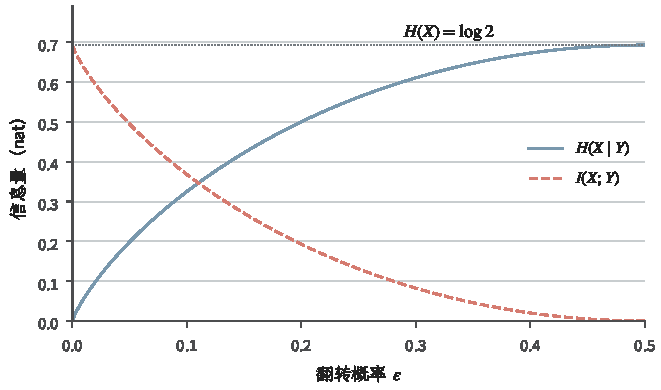
\includegraphics[width=\linewidth]{figures/01-mathematical-preliminaries/04-random-variables-distributions-and-causality/matplotlib/concepts-probability/information-binary-channel-information.pdf}
  \caption{公平二元输入通过独立翻转通道后的信息分配（解析式教学图）。蓝实线为剩余条件熵\(H_{\mathrm b}(\varepsilon)\)，红虚线为互信息\(\log2-H_{\mathrm b}(\varepsilon)\)，均以nat计。输入熵保持不变，零噪声与公平翻转分别对应完整信息与零信息。}
  \label{fig:information-binary-channel-information}
\end{figure}
由于对两个变量分别施加可逆变换会同时推送联合分布与边缘乘积，
互信息继承KL的不变性。这与微分熵随坐标单位改变形成区别。

\subsubsection{条件关系的互信息}
\label{sec:information-conditional-mi}

已经知道\(Z\)时，应在同一个条件值下判断\(X,Y\)是否还有关系，
再按\(Z\)的发生概率平均。不能把三者的边缘依赖随意相减。

\begin{definition}[条件互信息]
\label{def:information-conditional-mi}
设\(X,Y,Z\)取值于标准Borel空间，因而存在所需正则条件分布。
\term{条件互信息}（conditional mutual information）定义为
\begin{equation}
  I(X;Y\mid Z)
  =\int D_{\mathrm{KL}}\bigl(
    P_{XY\mid z}\Vert P_{X\mid z}\otimes P_{Y\mid z}\bigr)\,P_Z(\mathrm dz).
  \label{eq:information-conditional-mutual-information}
\end{equation}
条件核的版本只需在\(P_Z\)-几乎处处确定；被积量非负，允许结果为\(+\infty\)。
\end{definition}

在不保证正则条件分布存在的一般空间上，不能不加条件地沿用这个条件核定义。
在上述条件下，零条件互信息等价于条件联合核几乎处处等于条件边缘乘积，
也就是前章的条件独立。有限熵时可写成
\(H(X\mid Z)-H(X\mid Y,Z)\)，但非负KL积分是避免无穷相减的基本口径。

条件化并不一定使互信息变小。取独立公平二元变量\(X,Y\)，令\(Z=X\oplus Y\)。
边缘上互信息为零；固定\(Z\)后，\(X\)完全决定\(Y\)，条件互信息为\(\log2\)。
反过来，若\(X=Y=Z\)为同一个公平二元变量，无条件互信息为\(\log2\)，
条件互信息却为零。前者揭示约束，后者去掉已经知道的共享信息。

后处理和序贯观测都要用到KL的条件分解。设联合规律\(P_{AB},Q_{AB}\)
满足相应绝对连续性，条件核存在。联合密度比分解为边缘比与条件比的乘积，
取对数并用塔式性质得到
\begin{equation}
  D_{\mathrm{KL}}(P_{AB}\Vert Q_{AB})
  =D_{\mathrm{KL}}(P_A\Vert Q_A)
   +\mathbb E_{A\sim P_A}
       D_{\mathrm{KL}}(P_{B\mid A}\Vert Q_{B\mid A}).
  \label{eq:information-kl-conditional-chain}
\end{equation}
每个对数比的负部可积，故有限项相加的分解也能按非负扩展值成立；
若绝对连续性失败，对应的条件或边缘项为无限。
把\(Q_{XYZ}\)选为\(P_X\otimes P_{YZ}\)，再按\((X,Y)\)与\(Z\)分组，
第一项是\(I(X;Y)\)，条件项是
\(\mathbb E_{X,Y}D_{\mathrm{KL}}(P_{Z\mid X,Y}\Vert P_{Z\mid Y})
=I(X;Z\mid Y)\)。因此
\[
  I(X;Y,Z)=I(X;Y)+I(X;Z\mid Y).
\]
这证明了互信息链式法则，而不仅是引用熵差记号。

\begin{theorem}[数据处理不等式]
\label{thm:information-data-processing}
若标准Borel随机元素满足Markov关系\(X\to Y\to Z\)，
即\(X\perp Z\mid Y\)，则\(I(X;Z)\leq I(X;Y)\)，允许扩展值。
\end{theorem}
\begin{proof}
用两种顺序分解同一联合信息量：
\[
\begin{aligned}
  I(X;Y,Z)&=I(X;Y)+I(X;Z\mid Y)=I(X;Y),\\
  I(X;Y,Z)&=I(X;Z)+I(X;Y\mid Z)\geq I(X;Z).
\end{aligned}
\]
第一行的条件项由条件独立为零，第二行的条件项非负，合并即得。
证明只作非负项的相加和比较，不需要有限熵，也没有无穷相减。
\end{proof}

处理可以是\(Z=g(Y)\)，也可以是仅依赖\(Y\)的随机通道。
若额外随机性还与\(X\)关联，Markov前提可能不成立。
信息不增加并不保证每个任务的误差严格增加；当丢弃的内容与任务无关时可以取等号。

\subsection{分布差异的比较尺度}
\label{sec:information-distribution-discrepancies}

预测评分关心对数代价，越界报警关心事件概率，温度误差还关心数值相距多远。
这些要求未必由同一个散度直接表达。下面按允许观察的对象选择比较尺度；
它们可以重合，例如某些搬运距离也能写成测试函数的期望差。

\subsubsection{概率权重的差异}
\label{sec:information-probability-discrepancy}

报警规则由一个事件\(A\)指定。若尚未决定具体规则，可以问所有事件中，
哪一个的发生概率改变最多。

\begin{definition}[总变差距离]
\label{def:information-total-variation}
同一可测空间上概率测度的\term{总变差距离}（total variation distance, TV）为
\begin{equation}
  d_{\mathrm{TV}}(P,Q)=\sup_A|P(A)-Q(A)|,
  \label{eq:information-total-variation}
\end{equation}
其中上确界遍历全部可测事件。
\end{definition}

取共同支配测度\(\mu\)，密度为\(p,q\)。
由于\(\int(p-q)\,\mathrm d\mu=0\)，正部与负部积分相等。
任意事件上的差不超过正部积分，而\(A^\star=\{p\geq q\}\)达到该值，所以
\begin{equation}
  d_{\mathrm{TV}}(P,Q)=\tfrac12\int|p-q|\,\mathrm d\mu
   =P(A^\star)-Q(A^\star).
  \label{eq:information-tv-density}
\end{equation}
对\(|f|\leq1\)，积分的绝对值不超过\(\int|p-q|\)；
取\(f=2\mathbb I_{A^\star}-1\)达到上界，故
\begin{equation}
  2d_{\mathrm{TV}}(P,Q)
   =\sup_{\|f\|_\infty\leq1}|\mathbb E_Pf-\mathbb E_Qf|.
  \label{eq:information-tv-dual}
\end{equation}
若\(0\leq f\leq1\)，令\(g=2f-1\)，相应上确界则恰为\(d_{\mathrm{TV}}\)。
事件指标给出取等号的函数。这两个常数的差别来自值域宽度，不是定义冲突。

有时需要对称地比较密度形状，又希望使用Hilbert空间的几何。
把密度开平方便得到单位\(L^2\)范数的函数。

\begin{definition}[Hellinger距离]
\label{def:information-hellinger-distance}
在共同支配测度\(\mu\)下，定义平方\term{Hellinger距离}为
\begin{equation}
  d_{\mathrm H}^2(P,Q)=\tfrac12\int(\sqrt p-\sqrt q)^2\,\mathrm d\mu
   =1-\int\sqrt{pq}\,\mathrm d\mu,
  \label{eq:information-hellinger}
\end{equation}
距离本身为其非负平方根。
\end{definition}
更换共同支配测度时，两个平方根都乘以同一密度因子的平方根，
积分换元后不变。对三个分布可统一使用其和作支配测度，
从\(L^2\)三角不等式得到\(d_{\mathrm H}\)的三角不等式。
利用
\(|p-q|=|\sqrt p-\sqrt q|(\sqrt p+\sqrt q)\)，有
\[
  d_{\mathrm H}^2(P,Q)\leq d_{\mathrm{TV}}(P,Q)
  \leq\sqrt2\,d_{\mathrm H}(P,Q).
\]
左侧用\(\sqrt p+\sqrt q\geq|\sqrt p-\sqrt q|\)；
右侧用Cauchy--Schwarz以及
\(\int(\sqrt p+\sqrt q)^2\,\mathrm d\mu\leq4\)。

\begin{theorem}[Pinsker不等式]
\label{thm:information-pinsker}
以自然对数定义KL时，
\begin{equation}
  d_{\mathrm{TV}}(P,Q)\leq
  \sqrt{\tfrac12D_{\mathrm{KL}}(P\Vert Q)}.
  \label{eq:information-pinsker}
\end{equation}
\end{theorem}
\begin{proof}
KL无限时无需证明；否则\(P\ll Q\)。令
\(A=\{\mathrm dP/\mathrm dQ\geq1\}\)、\(a=P(A)\)、\(b=Q(A)\)，
则\(a-b=d_{\mathrm{TV}}(P,Q)\)。
在\(A\)及其补集分别对密度比使用条件Jensen不等式，得到
\[
  D_{\mathrm{KL}}(P\Vert Q)\geq
  a\log\frac ab+(1-a)\log\frac{1-a}{1-b}.
\]
固定\(b\in(0,1)\)，右侧作为\(a\)的函数在\(a=b\)处值和一阶导数为零，
二阶导数为\(1/[a(1-a)]\geq4\)。Taylor积分余项给出至少\(2(a-b)^2\)。
端点通过连续延拓处理；若\(b=0\)或\(1\)，有限KL迫使相应\(a=b\)。
整理即得结论。
\end{proof}

取\(P=\operatorname{Bernoulli}(1/4)\)、\(Q=\operatorname{Bernoulli}(1/2)\)，
则
\[
  d_{\mathrm{TV}}=\tfrac14,\qquad
  d_{\mathrm H}^2\approx0.0341,\qquad
  D_{\mathrm{KL}}(P\Vert Q)\approx0.1308.
\]
Pinsker给出的上界约为\(0.2557\)。这个控制不能反用：
\(P=(1-\eta)\delta_0+\eta\delta_1\)、\(Q=\delta_0\)的总变差只有\(\eta\)，
但只要\(\eta>0\)，前向KL就无限。

KL平均对数密度比；如果要限制极端密度比给事件概率带来的放大，
则可以直接控制更高阶矩。

\begin{definition}[高于一阶的Rényi散度]
\label{def:information-renyi-divergence}
对\(\alpha>1\)及\(P\ll Q\)，\term{R\'enyi散度}定义为
\begin{equation}
  D_\alpha(P\Vert Q)
   =\frac1{\alpha-1}\log\mathbb E_Q
       \left[\left(\frac{\mathrm dP}{\mathrm dQ}\right)^\alpha\right].
  \label{eq:information-renyi-divergence}
\end{equation}
若绝对连续性失败或该阶矩无限，结果为\(+\infty\)。
\end{definition}

令\(L=\mathrm dP/\mathrm dQ\)，Jensen给出
\(\mathbb E_Q L^\alpha\geq(\mathbb E_QL)^\alpha=1\)，故散度非负。
为了比较不同阶数，需要把定理~\ref{thm:linear-algebra-holder}的有限坐标配对
推广到函数积分。若\(1\leq p,q\leq\infty\)、\(1/p+1/q=1\)，且相应范数有限，则
\begin{equation}
 \int|uv|\,\mathrm d\mu\leq
 \|u\|_{L^p(\mu)}\|v\|_{L^q(\mu)}.
 \label{eq:information-integral-holder}
\end{equation}
这就是积分形式的Hölder不等式。对\(1<p,q<\infty\)，当两个范数非零时，
将\(|u|\)、\(|v|\)分别除以自己的范数，再逐点使用上述定理证明中的Young不等式并积分；
右侧归一化后为\(1/p+1/q=1\)，恢复尺度即得本式。
范数为零时相应函数几乎处处为零；端点\(p=1,q=\infty\)直接用
\(|v|\leq\|v\|_{L^\infty}\)几乎处处成立，另一端点交换两者。

取有限矩对应的\(a,b\geq1\)与\(0<t<1\)，对
\(u=L^{ta}\)、\(v=L^{(1-t)b}\)使用指数\(p=1/t\)、\(q=1/(1-t)\)，得到
\[
 \mathbb E_Q L^{ta+(1-t)b}
 \leq(\mathbb E_Q L^a)^t(\mathbb E_Q L^b)^{1-t}.
\]
取对数便说明\(K(\alpha)=\log\mathbb E_QL^\alpha\)在有限区间上为凸函数；
连同无穷值约定，它是扩展实值凸函数。
又因\(K(1)=0\)，割线斜率\(K(\alpha)/(\alpha-1)\)随阶数不减。
若某个\(\alpha_0>1\)的阶矩有限，则从右侧趋于一时可对矩函数求导，
得到\(D_\alpha\to\mathbb E_Q L\log L=D_{\mathrm{KL}}\)。
更大的阶数更强调大密度比，而不是更大的空间位移。
对上述Bernoulli例，\(\mathbb E_QL^2=1.25\)，
所以\(D_2=\log1.25\approx0.2231\)，高于KL。
事件迁移将在第~\ref{sec:information-bounded-evaluation}节使用这一阶矩；
重复机制的组合需要另外检查独立性或条件界。

\subsubsection{测试函数的期望差异}
\label{sec:information-test-functions}

如果任务只计算指定的一类函数，控制所有可测事件可能超出需要。
可以把每个允许的测试函数当作一种观测，再比较它在两个分布下的平均读数。

\begin{definition}[积分概率度量]
\label{def:information-ipm}
给定非空实值可测函数类\(\mathcal F\)，并假设每个成员在\(P,Q\)下可积，
相应的\term{积分概率度量}（integral probability metric, IPM）为
\begin{equation}
  d_{\mathcal F}(P,Q)=\sup_{f\in\mathcal F}
           |\mathbb E_Pf-\mathbb E_Qf|.
  \label{eq:information-ipm}
\end{equation}
\end{definition}
它对称并满足三角不等式，但可能为无限；如果函数类不能区分分布，
零值也可能对应不同分布，因而只给出伪距离。
选择\(\|f\|_\infty\leq1\)得到两倍TV。
选择核空间的单位球，则把比较限制为该核能够表示的函数。

\begin{definition}[最大均值差异]
\label{def:information-mmd}
设\(\mathcal H\)为再生核Hilbert空间，核\(k\)可测，且
\[
  \mathbb E_P\sqrt{k(X,X)}<\infty,\qquad
  \mathbb E_Q\sqrt{k(Y,Y)}<\infty.
\]
\term{最大均值差异}（maximum mean discrepancy, MMD）定义为
\[
  \operatorname{MMD}(P,Q)=
   \sup_{\|f\|_{\mathcal H}\leq1}|\mathbb E_Pf-\mathbb E_Qf|.
\]
\end{definition}

第~\ref{chap:functional-analysis-and-approximation}章的再生性质给出
\(|f(x)|\leq\|f\|_{\mathcal H}\sqrt{k(x,x)}\)，
所以\(f\mapsto\mathbb E_Pf\)是有界线性泛函。
Riesz表示定理保证存在唯一代表元\(\bm\mu_P\in\mathcal H\)，使
\(\mathbb E_Pf=\langle f,\bm\mu_P\rangle_{\mathcal H}\)。
这就是核均值（kernel mean embedding）：一张分布对全部核函数的平均作用。
不必预先假定Hilbert值积分存在；记号\(\mathbb E_Pk(X,\cdot)\)可由这个代表元解释。
对\(Q\)同理，于是
\[
  \operatorname{MMD}(P,Q)
  =\sup_{\|f\|_{\mathcal H}\leq1}
     |\langle f,\bm\mu_P-\bm\mu_Q\rangle|
  =\|\bm\mu_P-\bm\mu_Q\|_{\mathcal H}.
\]
差非零时取其归一化方向达到上确界。对可测有界核，所需可积条件自动满足。

\begin{definition}[核的特征性]
\label{def:information-characteristic-kernel}
在核均值均存在的指定分布类\(\mathcal P\)上，若
\(\bm\mu_P=\bm\mu_Q\)蕴含\(P=Q\)，即核均值映射为单射，
则称核\(k\)在\(\mathcal P\)上具有特征性（characteristic）。
\end{definition}

零MMD能否推出同分布，取决于这个条件。取同一对分布
\(P=\delta_0\)、\(Q=(\delta_{-1}+\delta_1)/2\)。
线性核\(k(x,y)=xy\)只比较普通均值，故MMD为零，
但\(P(\{0\})=1\)、\(Q(\{0\})=0\)。
改用高斯核\(k(x,y)=e^{-(x-y)^2/2}\)，展开核均值范数并用独立副本可得
\[
\begin{aligned}
  \operatorname{MMD}^2(P,Q)
  &=\mathbb E_{P\otimes P}k+\mathbb E_{Q\otimes Q}k
      -2\mathbb E_{P\otimes Q}k\\
  &=\tfrac32+\tfrac12e^{-2}-2e^{-1/2}>0.
\end{aligned}
\]
矩条件通过\(|k(x,y)|\leq\sqrt{k(x,x)k(y,y)}\)保证展开中的积分可交换。
图~\ref{fig:information-kernel-distinguishability}固定这两个分布，只改变核。
该算例证明高斯核能区分这一对对象，不代替整个分布类上的特征性证明。
\begin{figure*}[htbp]
  \centering
  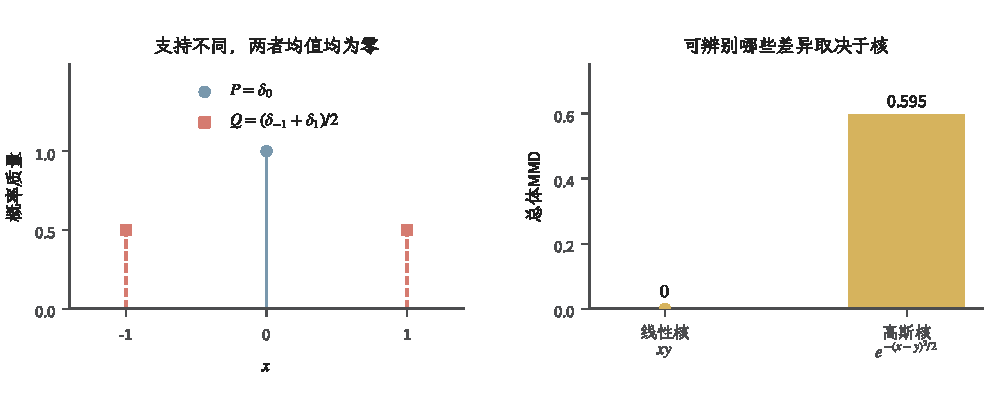
\includegraphics[width=\linewidth]{figures/01-mathematical-preliminaries/04-random-variables-distributions-and-causality/matplotlib/teaching-linear-probability/information-kernel-distinguishability.pdf}
  \caption{同均值分布在不同核下的MMD（解析式教学图）。左图为\(P=\delta_0\)与\(Q=(\delta_{-1}+\delta_1)/2\)，右图按精确总体期望计算：线性核给出零，高斯核给出约\(0.595\)。没有使用有限样本估计；差别来自测试函数类。}
  \label{fig:information-kernel-distinguishability}
\end{figure*}

\subsubsection{质量位置的搬运差异}
\label{sec:information-optimal-transport}

相邻两个点质量完全不重叠，TV已达到一，KL无限；但若结果只是温度读数，
把全部质量移动\(0.01\)度仍应属于小变化。
需要把样本空间的位置关系纳入比较。\term{最优传输}
（optimal transport, OT）寻找保持两边概率不变的最便宜配对
\scite{math-villani2009transport}

\begin{definition}[耦合]
\label{def:information-coupling}
给定\((\mathcal X,\mathcal A)\)、\((\mathcal Y,\mathcal B)\)上的概率测度\(P,Q\)，
其\term{耦合}（coupling）是乘积空间上的概率测度\(\gamma\)，满足
\[
  \gamma(A\times\mathcal Y)=P(A),\qquad
  \gamma(\mathcal X\times B)=Q(B).
\]
全体耦合记为\(\Pi(P,Q)\)。
\end{definition}
耦合规定一单位来源质量与哪部分目标质量配对，不改变两边总量。
独立耦合\(P\otimes Q\)总存在，但不一定便宜。
给定非负可测成本\(c(x,y)\)，Kantorovich搬运代价为
\begin{equation}
  \mathcal T_c(P,Q)=\inf_{\gamma\in\Pi(P,Q)}
                      \int c(x,y)\,\mathrm d\gamma(x,y).
  \label{eq:information-kantorovich-transport}
\end{equation}
下确界能否达到及怎样求解留到第~\ref{sec:information-coupling-optimization}节。
这里先把搬运用于比较分布。

\begin{definition}[Wasserstein距离]
\label{def:information-wasserstein-distance}
设\((\mathcal X,d)\)为完备可分度量空间，
\(1\leq r<\infty\)，固定基点\(x_0\)并令
\[
  \mathcal P_r(\mathcal X)=
   \left\{P:\int d(x,x_0)^r\,\mathrm dP(x)<\infty\right\}.
\]
对\(P,Q\in\mathcal P_r(\mathcal X)\)，定义
\begin{equation}
  W_r(P,Q)=\left[
    \inf_{\gamma\in\Pi(P,Q)}\int d(x,y)^r\,\mathrm d\gamma(x,y)
  \right]^{1/r}.
  \label{eq:information-wasserstein-distance}
\end{equation}
\end{definition}

由\(d(x,x_1)^r\leq2^{r-1}\{d(x,x_0)^r+d(x_0,x_1)^r\}\)，
矩条件不依赖基点；同一不等式说明独立耦合的成本有限。
对称性来自底层距离，对角耦合给出\(W_r(P,P)=0\)。
若\(W_r(P,Q)=0\)，任意有界\(L\)-Lipschitz函数的期望差至多
\(L(\mathbb E_\gamma d(X,Y)^r)^{1/r}\)，沿近最优耦合趋于零。
用连续函数\(\max\{1-kd(x,C),0\}\)逼近闭集\(C\)的指标，得到所有闭集上
\(P(C)=Q(C)\)，故\(P=Q\)。

三角不等式需要先控制随机距离之和。对\(u,v\in L^r(\mu)\)，这里使用Minkowski不等式
\(\|u+v\|_{L^r}\leq\|u\|_{L^r}+\|v\|_{L^r}\)。
它仍沿用有限维的证明：\(r=1\)直接对绝对值三角不等式积分；
\(1<r<\infty\)时，先由
\(|u+v|^r\leq2^{r-1}(|u|^r+|v|^r)\)确认\(u+v\in L^r\)，再写
\[
 \|u+v\|_{L^r}^r
 \leq\int|u+v|^{r-1}(|u|+|v|)\,\mathrm d\mu
 \leq\|u+v\|_{L^r}^{r-1}(\|u\|_{L^r}+\|v\|_{L^r}).
\]
末步对两项分别使用式~\eqref{eq:information-integral-holder}，指数为
\(r/(r-1)\)与\(r\)。非零时约去公共幂，零时结论直接成立。

还需把两个配对接起来。把\(P,Q\)的耦合分解为
\(P(\mathrm dx\mid y)Q(\mathrm dy)\)，把\(Q,R\)的耦合分解为
\(Q(\mathrm dy)R(\mathrm dz\mid y)\)。Polish空间上的正则条件分布允许构造
\[
  P(\mathrm dx\mid y)Q(\mathrm dy)R(\mathrm dz\mid y),
\]
其相邻边缘正是原来的两张耦合。这是粘合引理在这里的具体实现。
由\(d(X,Z)\leq d(X,Y)+d(Y,Z)\)及Minkowski不等式，
\[
  \bigl(\mathbb E d(X,Z)^r\bigr)^{1/r}
  \leq\bigl(\mathbb E d(X,Y)^r\bigr)^{1/r}
       +\bigl(\mathbb E d(Y,Z)^r\bigr)^{1/r}.
\]
分别选近最优耦合并令误差趋零，就得到\(W_r(P,R)\leq W_r(P,Q)+W_r(Q,R)\)。
一般成本\(c\)不具备这些距离性质，\(\mathcal T_c\)不能自动称为距离；
超出矩条件时，扩展定义还可能为无限。

对有限一阶矩的\(P,Q\)，Kantorovich--Rubinstein对偶给出
\begin{equation}
  W_1(P,Q)=\sup_{\operatorname{Lip}(f)\leq1}
                         |\mathbb E_Pf-\mathbb E_Qf|.
  \label{eq:information-kr-duality}
\end{equation}
其中\(\operatorname{Lip}(f)\leq1\)表示\(|f(x)-f(y)|\leq d(x,y)\)。
可以固定\(f(x_0)=0\)，不改变期望差，且一阶矩保证可积。
任意耦合都给出右侧不超过左侧；反向是最优传输对偶定理的实质内容，
这里按上述Polish及矩条件使用。有限空间的完整线性规划对偶将在后文推导。
这说明\(W_1\)也是IPM；\(r>1\)的\(W_r\)没有这里同一个Lipschitz单位球表达。

用同方差高斯来比较三种尺度。令\(P=\mathcal N(\mu,\sigma^2)\)、
\(Q=\mathcal N(\nu,\sigma^2)\)。取\(Y=X+\nu-\mu\)得到恒定位移耦合，
而任意耦合满足
\(\mathbb E|X-Y|^2\geq|\mathbb EX-\mathbb EY|^2=|\mu-\nu|^2\)，故
\begin{equation}
  W_2(P,Q)=|\mu-\nu|.
  \label{eq:information-gaussian-location-wasserstein}
\end{equation}
若\(\mu<\nu\)，两密度在\(c=(\mu+\nu)/2\)相交，
\(P\)在\((-\infty,c]\)上的密度较大。因此
\[
  d_{\mathrm{TV}}(P,Q)
  =P((-\infty,c])-Q((-\infty,c])
  =2\Phi\left(\frac{|\mu-\nu|}{2\sigma}\right)-1.
\]
当\(|\mu-\nu|=0.2,\sigma=1\)时，\(W_2=0.2\)、KL为\(0.02\)、
TV约为\(0.0797\)。若标准差\(\sigma\)减半，搬运位移不变，KL增为\(0.08\)，TV也增大。
位置差与可辨别程度因此不能互换。

图~\ref{fig:information-gaussian-distances}保留同一位置族的三尺度对照，
面板纵轴不同，不能按曲线高度判断哪一种概念更强。
\begin{figure*}[htbp]
  \centering
  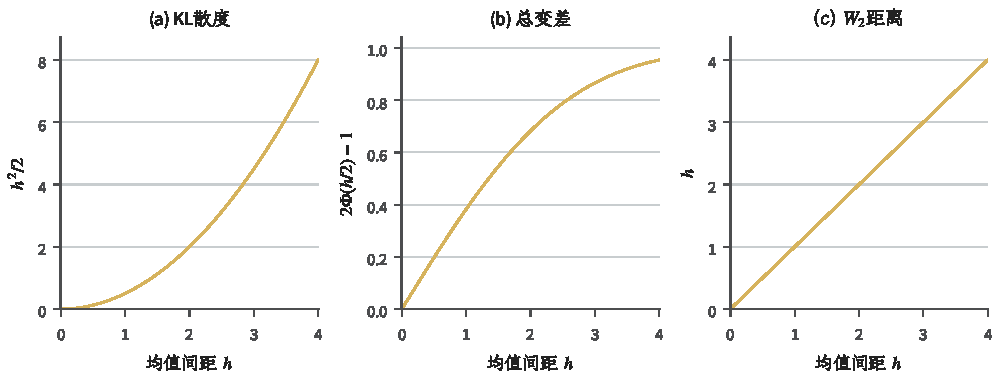
\includegraphics[width=\linewidth]{figures/01-mathematical-preliminaries/04-random-variables-distributions-and-causality/matplotlib/probability-discrete/information-gaussian-distances.pdf}
  \caption{同方差高斯位置族的解析式比较。固定\(P=\mathcal N(0,1)\)、\(Q=\mathcal N(h,1)\)，三图分别为\(D_{\mathrm{KL}}=h^2/2\)、\(d_{\mathrm{TV}}=2\Phi(h/2)-1\)与\(W_2=h\)，图中\(h\geq0\)。纵轴分别表达对数代价、事件概率差与搬运位移。}
  \label{fig:information-gaussian-distances}
\end{figure*}

对点质量\(\delta_0,\delta_\varepsilon\)，只要\(\varepsilon\neq0\)，
TV恒为一、两个方向KL均无限，而\(W_r=|\varepsilon|\to0\)。
这是支持移动在不同尺度下的极限差别。
对时间边缘分布\((P_t)\)也可比较这些距离，但它们不决定轨迹机制：
每时刻都为同一公平二元分布，既可能来自反复独立抽样，也可能来自把初次抽样永远复制。
两过程边缘距离为零，时间依赖却完全不同，必须比较联合轨迹。
实际估计MMD或Wasserstein还需考虑核、底层成本、矩和样本量；
高维经验搬运的估计误差可能很大，精确总体公式不自动给出便宜的样本估计。

\subsection{观测分布的可区分性}
\label{sec:information-lower-bounds}

分布差异也能说明推断的限度。若两个环境几乎产生相同观测，却要求不同答案，
任何程序都不能同时在两者上准确。这里固定所要恢复的目标和观测制度，
对所有估计程序给出下界；程序是否易于计算是另一问题。

\subsubsection{固定观测下的区分限制}
\label{sec:information-fixed-observations}

先把整批观测的分布视为已给定，不让程序根据中途结果改变取样位置。
两候选比较利用TV，多候选比较则需要把候选数量也纳入信息预算。

\paragraph{两个候选的区分下界}
\label{sec:information-two-candidates}

设观测\(Z\)来自\(P_0\)或\(P_1\)，先验各为\(1/2\)。
检验\(\psi(Z)\in\{0,1\}\)以事件\(A=\{\psi=1\}\)选择第二个候选，则错误和为
\[
  P_0(A)+P_1(A^{\mathsf c})=1-\{P_1(A)-P_0(A)\}.
\]
取使密度差为正的事件达到上确界，得到
\begin{equation}
  \inf_\psi\{P_0(\psi=1)+P_1(\psi=0)\}
     =1-d_{\mathrm{TV}}(P_0,P_1).
  \label{eq:information-binary-testing-tv}
\end{equation}
随机化检验只是把指标改为\([0,1]\)值函数，按TV的函数表达也不能降低这个值。
在等先验下，最小总体错误是右侧的一半；两类条件错误之和本身不是总体错误。

数值估计可以转成检验：若估计足够准，就应能知道它靠近哪个候选目标。

\begin{theorem}[Le Cam两点下界]
\label{thm:information-le-cam}
设观测模型\(P_0,P_1\)对应目标\(\theta_0,\theta_1\)，
在目标空间度量\(d\)下有\(d(\theta_0,\theta_1)\geq2s\)，\(s>0\)。
任意估计量\(\widehat\theta\)均满足
\begin{equation}
  \max_{j\in\{0,1\}}P_j\{d(\widehat\theta,\theta_j)\geq s\}
  \geq\frac{1-d_{\mathrm{TV}}(P_0,P_1)}2.
  \label{eq:information-le-cam}
\end{equation}
\end{theorem}
\begin{proof}
构造最近目标检验
\(\psi=\mathbb I\{d(\widehat\theta,\theta_1)<d(\widehat\theta,\theta_0)\}\)，
距离相等时选\(0\)。若真实为\(0\)且估计误差小于\(s\)，由三角不等式，
估计与\(\theta_1\)的距离大于\(s\)，检验不会错。
真实为\(1\)时同理。因此检验错误分别包含在估计坏事件内。
两个坏事件概率之和至少为\(1-d_{\mathrm{TV}}(P_0,P_1)\)，
其中最大者至少为一半，即得结论。
\end{proof}

若每个候选下都得到\(n\)个独立同分布观测，联合密度比是单次密度比的乘积，
取对数并平均得到
\(D_{\mathrm{KL}}(P_0^{\otimes n}\Vert P_1^{\otimes n})
=nD_{\mathrm{KL}}(P_0\Vert P_1)\)。
取单次规律为\(\mathcal N(-a,\sigma^2)\)与\(\mathcal N(a,\sigma^2)\)，
目标均值相距\(2a\)，整批KL为\(2na^2/\sigma^2\)。
令\(a=\sigma/(2\sqrt n)\)，KL为\(1/2\)，Pinsker给出TV至多\(1/2\)。
所以任何均值估计量都至少在一个候选下，以不小于\(1/4\)的概率产生
不小于\(\sigma/(2\sqrt n)\)的绝对误差。
若评价平方误差，还可由这个事件下界得到最坏风险至少\(\sigma^2/(16n)\)。
这些常数来自所选两点及放缩，不声称最优。

\paragraph{多个候选的区分下界}
\label{sec:information-many-candidates}

两点只要求区分一个二元选择；高维问题可能同时包含许多不同目标。
令\(V\)在\(\{1,\ldots,M\}\)上均匀，给定\(V=v\)后观测\(Z\sim P_v\)。
解码器\(\widehat V(Z)\)的错误概率记为\(p_{\mathrm e}\)。
即使\(Z\)连续，\(V\)的条件熵仍可按其有限后验概率求熵，再对\(Z\)积分。

\begin{theorem}[Fano不等式]
\label{thm:information-fano}
对\(M\geq2\)及上述观测模型，
\begin{equation}
  p_{\mathrm e}\geq1-\frac{I(V;Z)+\log2}{\log M}.
  \label{eq:information-fano}
\end{equation}
\end{theorem}
\begin{proof}
令\(E=\mathbb I\{\widehat V\neq V\}\)。给定\(Z\)且\(E=0\)时，
\(V=\widehat V(Z)\)已确定；给定\(E=1\)时，至多还有\(M-1\)个可能索引。
有限字母表上最大熵为均匀熵，这也可由与均匀分布的Gibbs不等式得到。
于是
\[
\begin{aligned}
  H(V\mid Z)
  &\leq H(V,E\mid Z)\\
  &=H(E\mid Z)+H(V\mid E,Z)\\
  &\leq\log2+p_{\mathrm e}\log(M-1)
   \leq\log2+p_{\mathrm e}\log M.
\end{aligned}
\]
又因\(H(V)=\log M\)，互信息分解给出
\(H(V\mid Z)=\log M-I(V;Z)\)。移项得到结论。
随机化解码可把独立随机种子并入\(Z\)，不会增加关于\(V\)的信息。
\end{proof}

若目标集合中有两两距离至少\(2s\)的有限分离集
\(\{\theta_1,\ldots,\theta_M\}\)，误差小于\(s\)就能最近邻解码。
这把前面计数与打包的工具接到统计下界：候选多能提高\(\log M\)，
但必须同时控制观测中含有多少索引信息\scite{math-cover2006information}
令\(\overline P=M^{-1}\sum_uP_u\)，则
\[
  I(V;Z)=\frac1M\sum_vD_{\mathrm{KL}}(P_v\Vert\overline P)
  \leq\frac1{M^2}\sum_{v,u}D_{\mathrm{KL}}(P_v\Vert P_u).
\]
等式来自给定\(V\)的条件KL分解；不等式来自
\(-\log(M^{-1}\sum_u p_u)\leq M^{-1}\sum_u(-\log p_u)\)。
因此
\(\max_vP_v\{d(\widehat\theta,\theta_v)\geq s\}\)
至少为Fano右侧，若右侧为负则只得到平凡下界零。

保留一个可复算的四候选构造：均值为\(\{-3a,-a,a,3a\}\)，
每个候选产生\(n\)个方差\(\sigma^2\)的独立高斯观测。
最小间距为\(2a\)，有序候选对的平均平方距离为\(10a^2\)，故
\[
  I(V;Z)\leq\frac{5na^2}{\sigma^2}.
\]
取\(a=\sigma/(4\sqrt n)\)时右侧为\(5/16\)，Fano给出
\(p_{\mathrm e}\geq1-(5/16+\log2)/\log4\approx0.2746\)。
任意估计器因此至少在一个候选上以这一概率产生不小于\(a\)的误差。
目标分离与观测接近必须同时成立；只罗列许多模型不构成下界证明。

\subsubsection{序贯观测下的区分限制}
\label{sec:information-sequential-observations}

若观测位置根据已获得的结果改变，最终资料的联合分布也随算法改变。
仍可使用前面的检验不等式，但比较对象应当是包含行动与结果的完整轨迹。

\paragraph{重复与时序观测的信息累积}
\label{sec:information-sequential-accumulation}

独立重复是简单情形。设对应分量满足绝对连续性，密度比为\(L_t\)。
乘积规律的比值为\(\prod_tL_t\)，因此
\[
\begin{aligned}
  D_{\mathrm{KL}}\left(\bigotimes_tP_t\Big\Vert\bigotimes_tQ_t\right)
     &=\sum_tD_{\mathrm{KL}}(P_t\Vert Q_t),\\
  D_\alpha\left(\bigotimes_tP_t\Big\Vert\bigotimes_tQ_t\right)
     &=\sum_tD_\alpha(P_t\Vert Q_t),\qquad\alpha>1.
\end{aligned}
\]
第一式由对数把乘积化为和；第二式由独立性使
\(\mathbb E_{\otimes Q_t}\prod_tL_t^\alpha=\prod_t\mathbb E_{Q_t}L_t^\alpha\)。
公式可按扩展值理解，不通过相减处理无限项。

一般序列不独立。设\(Z_{0:T}\)在标准Borel空间取值，两个规律分解为初始分布及
历史条件核，\(P_0\ll Q_0\)，且在相关的\(P\)-历史上
\(P_t(\cdot\mid Z_{<t})\ll Q_t(\cdot\mid Z_{<t})\)。
前章条件换测度给出联合密度比
\[
  L_{0:T}=L_0(Z_0)\prod_{t=1}^T L_t(Z_t\mid Z_{<t}).
\]
对数相加，再对每一项先按历史条件平均，得到
\begin{equation}
\begin{aligned}
 D_{\mathrm{KL}}(P_{0:T}\Vert Q_{0:T})
 &=D_{\mathrm{KL}}(P_0\Vert Q_0)\\
 &\quad+\sum_{t=1}^T\mathbb E_{Z_{<t}\sim P}
 D_{\mathrm{KL}}\bigl(P_t(\cdot\mid Z_{<t})
                     \Vert Q_t(\cdot\mid Z_{<t})\bigr).
\end{aligned}
\label{eq:information-trajectory-kl-chain}
\end{equation}
这是式~\eqref{eq:information-kl-conditional-chain}的反复应用。
有限时域中每个条件对数比的负部积分均有统一有限界，
故可合法按扩展值累加；得到有限数值则还需累计条件KL有限。
期望必须沿前向分布\(P\)实际产生的历史计算。

轨迹包含行动时，同一算法在同一历史上使用相同的条件行动核，
所以比较两个环境时行动因子相消；两个环境的历史频率却不会相消。
在同一环境比较两条策略时，则是环境核相消，剩下条件行动KL。
若两者都改变，不能省略其中任何一组项。

Rényi不能把条件散度直接按\(P\)平均。一个充分组合条件是，对每个相关历史都有
确定的统一界
\[
  D_\alpha(P_t(\cdot\mid h_{<t})\Vert Q_t(\cdot\mid h_{<t}))
  \leq\varepsilon_t.
\]
为简化记号从\(t=1\)开始且初始历史固定。在\(Q\)下从最后一步取条件期望，
\[
  \mathbb E_Q[L_t^\alpha\mid h_{<t}]
       \leq e^{(\alpha-1)\varepsilon_t}.
\]
前面的密度比是历史可测量，因此每消去一步至多乘上这个常数。
反复迭代后
\[
  \mathbb E_Q L_{1:T}^{\alpha}
  \leq e^{(\alpha-1)\sum_t\varepsilon_t},\qquad
  D_\alpha(P_{1:T}\Vert Q_{1:T})\leq\sum_t\varepsilon_t.
\]
若只在某种历史分布下给出平均条件界，后续选择可能偏向高散度历史，
不能据此使用这个组合结论。

固定有限时域无需停止论证。若共同停止规则给出\(\tau\leq T\)，
停止后补同一个吸收符号，其条件信息代价为零，公式仍适用。
无界停时则应确认在所比较的规律下几乎处处终止；
一种足够的取极限条件是截断累计对数似然比
\(\log L_{0:\tau\wedge n}\)在\(P\)下均匀可积并收敛到停止轨迹的对数密度比。
此时左侧期望可取极限，右侧的非负条件KL用单调收敛。
终止本身不能代替这些可积条件。
隐私分析若使用组合式，还必须另外规定相邻输入、随机机制，
以及对全部相邻输入统一成立的界；单个分布对的散度不是完整隐私定义。

\paragraph{自适应观测的区分下界}
\label{sec:information-adaptive-lower-bounds}

设算法\(\mathcal A\)在时刻\(t\)根据历史选择来源或状态行动对\((s,a)\)，
观测核在环境\(j\)中为\(P_j(\cdot\mid s,a)\)。
若初始规律相同、条件行动规则相同，且观测在给定历史及当前\((s,a)\)后使用该核，
轨迹链式法则可按访问位置分组：
\[
  D_{\mathrm{KL}}(\mathbb P_0^{\mathcal A}\Vert\mathbb P_1^{\mathcal A})
  =\sum_{s,a}\mathbb E_0N_T(s,a)\,
      D_{\mathrm{KL}}(P_0(\cdot\mid s,a)\Vert P_1(\cdot\mid s,a)).
\]
这里\(N_T(s,a)\)为\(T\)步中的访问次数；等式来自
\(\sum_t\mathbb I\{(S_t,A_t)=(s,a)\}=N_T(s,a)\)。
它是由算法和环境共同产生的随机量，不能预先替换成均匀独立的样本数。
核若还依赖其他历史，保留逐步条件KL形式，不能强行按固定位置常数提取。

考虑两个可选Bernoulli来源\(A,B\)。环境\(0\)的均值为
\((1/2+\varepsilon,1/2)\)，环境\(1\)为
\((1/2+\varepsilon,1/2+2\varepsilon)\)，\(0<\varepsilon<1/4\)。
每次访问给出独立于过去的相应来源新观测，但来源选择允许自适应。
两个环境的最优来源相反，全部区分信息只来自\(B\)，单次KL为
\[
  \kappa(\varepsilon)
  =D_{\mathrm{KL}}\bigl(\operatorname{Bernoulli}(1/2)
             \Vert\operatorname{Bernoulli}(1/2+2\varepsilon)\bigr)
  =-\tfrac12\log(1-16\varepsilon^2).
\]
故轨迹KL为\(\mathbb E_0N_T(B)\kappa(\varepsilon)\)。
若输出的来源在两个环境下的错误都不超过\(\delta<1/2\)，
检验恒等式迫使TV至少为\(1-2\delta\)，Pinsker进一步给出
\[
  \mathbb E_0N_T(B)\geq
  \frac{2(1-2\delta)^2}{\kappa(\varepsilon)}.
\]
例如\(\varepsilon=0.1,\delta=0.1\)，有
\(\kappa\approx0.08718\)，期望访问至少约\(14.68\)次。
当\(\varepsilon\)小时，\(\kappa=8\varepsilon^2+O(\varepsilon^4)\)，
因此固定错误水平需要\(\varepsilon^{-2}\)量级的区分观测。
这是信息不足的预算下界，不是某个算法已达到该预算的上界。
推广到无界停止必须满足上一段的终止和可积条件；
更具体的价值或累计决策损失还要引入相应任务定义。

\section{随机分布扰动与任务稳定性}
\label{sec:information-task-stability}

同一个预测器在两个测试总体上运行，平均损失能相差多少？这个问题固定评价规则，
只改变数据分布。如果预测器又是从当前评价样本中挑选的，问题就多了一层：
较低的样本损失可能来自选择过程，而非真实风险降低。
下面先控制固定函数的期望变化，再把样本与算法输出的依赖纳入比较。

\subsection{固定评价下的期望稳定性}
\label{sec:information-fixed-evaluation}

取值范围、输入敏感程度和尾部条件，分别提供三种可以利用的信息。
一个函数可能同时有界、Lipschitz且具有次高斯尾部，因此以下工具可以比较后择优使用，
并不是三类互斥任务。

\subsubsection{有界函数下的期望变化}
\label{sec:information-bounded-evaluation}

设固定可测损失\(f\)取值于\([0,1]\)。逐点恒等式
\(f(x)=\int_0^1\mathbb I\{f(x)>t\}\,\mathrm dt\)与Tonelli定理给出
\[
  |\mathbb E_Pf-\mathbb E_Qf|
  \leq\int_0^1|P(f>t)-Q(f>t)|\,\mathrm dt
  \leq d_{\mathrm{TV}}(P,Q).
\]
这也说明事件概率控制为何足以控制所有这一范围内的损失。
若\(a\leq f\leq b\)，对\((f-a)/(b-a)\)使用同一式子，得到
\[
  |\mathbb E_Pf-\mathbb E_Qf|
  \leq(b-a)d_{\mathrm{TV}}(P,Q).
\]
特别地，\(|f|\leq1\)时常数是\(2\)，不能把它与\(0\leq f\leq1\)混用。
取两点上的\(P=\delta_0,Q=\delta_1\)和\(f(0)=-1,f(1)=1\)，
期望差为\(2\)，已经表明这个因子不能删除。
结合Pinsker，还可用\((b-a)\sqrt{D_{\mathrm{KL}}(P\Vert Q)/2}\)控制期望差；
若KL无限，这个途径不给出有限信息，但TV界仍有效。

对罕见失败事件，除了TV的加性误差，还可以利用似然比高阶矩。
设\(P\ll Q\)、\(L=\mathrm dP/\mathrm dQ\)，并且某个\(\alpha>1\)满足
\(D_\alpha(P\Vert Q)<\infty\)。由H\"older不等式，
\[
  P(A)=\mathbb E_Q[L\mathbb I_A]
  \leq(\mathbb E_QL^\alpha)^{1/\alpha}
       (\mathbb E_Q\mathbb I_A^{\alpha/(\alpha-1)})^{(\alpha-1)/\alpha}.
\]
代入R\'enyi散度定义，得到
\begin{equation}
  P(A)\leq
  \exp\!\left\{\frac{\alpha-1}{\alpha}D_\alpha(P\Vert Q)\right\}
  Q(A)^{(\alpha-1)/\alpha}.
  \label{eq:information-renyi-event-bound}
\end{equation}
若\(Q(A)=0\)，绝对连续直接给出\(P(A)=0\)，无需计算无穷与零的乘积。
若\(Q(A)=0<P(A)\)，所需方向的绝对连续已经失败，相应散度无限。
例如\(D_2(P\Vert Q)\leq\log4\)、\(Q(A)\leq10^{-4}\)时，
上界为\(2\sqrt{10^{-4}}=0.02\)。这是从参考规律\(Q\)到目标规律\(P\)
的单向风险迁移，不保证反向同样成立。

有界性不能只在常见样本上成立。取
\(Q=\delta_0\)、\(P_\varepsilon=(1-\varepsilon)\delta_0+
\varepsilon\delta_{1/\varepsilon}\)，对无界函数\(f(x)=x\)，
TV为\(\varepsilon\)，期望差却恒为\(1\)。少量尾部质量足以破坏
只依赖TV的小误差结论，必须另外控制函数增长或分布尾部。

\subsubsection{敏感性约束下的期望变化}
\label{sec:information-sensitive-evaluation}

若损失不会因输入小幅移动而剧变，就应让这种敏感性进入界。
设\(P,Q\in\mathcal P_1(\mathcal X)\)，且
\(|f(x)-f(y)|\leq Ld(x,y)\)。由于
\(|f(x)|\leq|f(x_0)|+Ld(x,x_0)\)，两边期望均有限。
任意耦合\(\gamma\in\Pi(P,Q)\)满足
\[
  |\mathbb E_Pf-\mathbb E_Qf|
  =\left|\int(f(x)-f(y))\,\mathrm d\gamma\right|
  \leq L\int d(x,y)\,\mathrm d\gamma.
\]
对耦合取下确界便得到
\[
  |\mathbb E_Pf-\mathbb E_Qf|\leq LW_1(P,Q).
\]
这也可由式~\eqref{eq:information-kr-duality}直接读出。
界不要求函数有界，但同时使用了一阶矩和相对于所选距离的Lipschitz条件。

对\(\delta_0,\delta_\varepsilon\)，其中\(\varepsilon>0\)，
均值函数\(f(x)=x\)的变化恰为\(\varepsilon=W_1\)，
事件函数\(g(x)=\mathbb I\{x>0\}\)的变化却为\(1\)。
后者在零附近不连续，不属于统一Lipschitz类。
图~\ref{fig:information-small-shift-task}把同一质量位移对应的这两种评价分开显示；
小搬运距离确实保护平滑评价，但不能据此声称所有阈值事件都稳定。
\begin{figure}[htbp]
  \centering
  % Exact schematic: delta_0 and delta_epsilon under two fixed test functions.
\begin{tikzpicture}[
  x=1mm,y=1mm,
  every node/.style={font=\figurefont\footnotesize,text=FigureInk,inner sep=1pt,fill=none},
  axis/.style={draw=FigureStroke,line width=.55pt,->},
  guide/.style={draw=FigureGrid,line width=.5pt,dashed},
  curve/.style={draw=FigureStroke,line width=.85pt}
]
  \path[use as bounding box] (0,0) rectangle (112,48);
  \node at (27,44) {\(f(x)=x\)};
  \node at (86,44) {\(g(x)=\mathbb I\{x>0\}\)};
  \draw[axis] (6,12) -- (49,12) node[above=3pt] {\(x\)};
  \draw[axis] (10,12) -- (10,36);
  \draw[curve] (8,11) -- (46,30);
  \draw[guide] (38,12) -- (38,26);
  \fill[FigureBlue] (10,12) circle (1.1mm);
  \fill[FigureRed] (38,26) circle (1.1mm);
  \node[below=2pt] at (10,12) {\(0\)};
  \node[below=2pt] at (38,12) {\(\varepsilon\)};
  \node[text=FigureBlue,above left=2pt] at (10,12) {\(P\)};
  \node[text=FigureRed,above left=2pt] at (38,26) {\(Q\)};
  \draw[<->,FigureMuted,line width=.6pt] (44,12.6) -- (44,25.4);
  \node[right] at (44,19) {\(\varepsilon\)};
  \node at (27,2) {期望差：\(\varepsilon\)};
  \draw[axis] (64,12) -- (109,12) node[above=3pt] {\(x\)};
  \draw[draw=FigureStroke,line width=.55pt] (68,12) -- (68,30.9);
  \draw[axis] (68,33.1) -- (68,37);
  \draw[curve] (64,12) -- (68,12);
  \draw[curve] (69.1,32) -- (106,32);
  \draw[guide] (96,12) -- (96,32);
  \draw[draw=FigureStroke,fill=none,line width=.7pt] (68,32) circle (1mm);
  \fill[FigureBlue] (68,12) circle (1.1mm);
  \fill[FigureRed] (96,32) circle (1.1mm);
  \node[below=2pt] at (68,12) {\(0\)};
  \node[below=2pt] at (96,12) {\(\varepsilon\)};
  \node[left=3pt] at (68,32) {\(1\)};
  \node[text=FigureBlue,above left=2pt] at (68,12) {\(P\)};
  \node[text=FigureRed,above=3pt] at (96,32) {\(Q\)};
  \node at (86,2) {期望差：\(1\)};
\end{tikzpicture}

  \caption{同一小位移对两种固定评价的影响。取\(P=\delta_0\)、
  \(Q=\delta_\varepsilon\)、\(\varepsilon>0\)，底层距离为绝对值。
  左图的\(1\)-Lipschitz函数\(f(x)=x\)变化\(\varepsilon\)；
  右图的事件函数\(\mathbb I\{x>0\}\)变化\(1\)。横向位置仅作示意，
  结论对任意正的\(\varepsilon\)成立。}
  \label{fig:information-small-shift-task}
\end{figure}

MMD提供另一种敏感性约束。若同一损失\(f\)属于核\(k\)的RKHS
\(\mathcal H_k\)，且核均值存在，则再生性质和Cauchy--Schwarz不等式给出
\[
  |\mathbb E_Pf-\mathbb E_Qf|
  =|\langle f,\bm\mu_P-\bm\mu_Q\rangle_{\mathcal H_k}|
  \leq\|f\|_{\mathcal H_k}\operatorname{MMD}_k(P,Q).
\]
下标\(k\)显式标明这里沿用的核空间和MMD。
必须知道\(f\)属于该空间及其范数；核具有特征性只保证分离分布，
不自动给出任意任务函数的有限范数。
同样，若底层成本只比较图像亮度，而任务依赖没有计入成本的位置变化，
不能声称损失相对于该成本是Lipschitz。成本与核是任务假设的一部分。

\subsubsection{指数矩条件下的期望变化}
\label{sec:information-change-measure}

有些损失没有统一上界，也难以给出输入空间的敏感常数，
但在参考分布下可控制其尾部。第~\ref{sec:rv-change-measure}节
允许用密度比换测度；下面用KL和指数矩代替密度比的逐点控制。
证明的关键是指数倾斜：按\(e^f\)重新加权参考分布，使较大函数值获得更多质量。

\begin{theorem}[Donsker--Varadhan变分表达]
\label{thm:information-donsker-varadhan}
设\(P\ll Q\)。对每个有界可测实函数\(f\)，
\begin{equation}
  D_{\mathrm{KL}}(P\Vert Q)
  \geq\mathbb E_Pf-\log\mathbb E_Qe^f.
  \label{eq:information-dv-lower}
\end{equation}
而且在扩展实数意义下，
\begin{equation}
  D_{\mathrm{KL}}(P\Vert Q)
  =\sup_{f\ \text{有界可测}}\{\mathbb E_Pf-\log\mathbb E_Qe^f\}.
  \label{eq:information-dv-variational}
\end{equation}
\end{theorem}
\begin{proof}
给定有界\(f\)，令\(Z_f=\mathbb E_Qe^f\)，并定义
\[
  \frac{\mathrm dQ_f}{\mathrm dQ}=\frac{e^f}{Z_f}.
\]
因\(0<Z_f<\infty\)，且密度比严格正，\(Q_f\)与\(Q\)等价。
若\(D_{\mathrm{KL}}(P\Vert Q)<\infty\)，对数密度比可积，
乘法法则给出完整的倾斜恒等式
\[
\begin{aligned}
  D_{\mathrm{KL}}(P\Vert Q_f)
  &=\mathbb E_P\left[\log\frac{\mathrm dP}{\mathrm dQ}-f+\log Z_f\right]\\
  &=D_{\mathrm{KL}}(P\Vert Q)-\mathbb E_Pf+\log Z_f.
\end{aligned}
\]
左侧非负即得下界；若原KL无限，右侧有限，下界仍成立。

为证明上确界恰好等于KL，不能直接假设\(\log(\mathrm dP/\mathrm dQ)\)有界。
记\(L=\mathrm dP/\mathrm dQ\)，在\(L=0\)处令\(\log L=-\infty\)，取
\[
  f_n=\max\{-n,\min\{\log L,n\}\}.
\]
由于\(P(L=0)=0\)，且
\(\mathbb E_P(\log L)^-=\int_{\{L<1\}}-L\log L\,\mathrm dQ<\infty\)，
负部由支配收敛、正部由单调收敛可知
\(\mathbb E_Pf_n\to D_{\mathrm{KL}}(P\Vert Q)\)，允许极限无限。
另一方面，\(e^{f_n}\to L\)，且\(e^{f_n}\leq1+L\)。
在\(Q\)下支配收敛给出\(\mathbb E_Qe^{f_n}\to1\)，
故对应变分值趋向KL。结合已证上界，得到等式。
若\(\log L\)本身有界，它直接取到等号；一般只保证截断序列逼近。
\end{proof}

取两点均匀参考分布\(Q=(1/2,1/2)\)，\(f=(0,\log3)\)，则
\(Z_f=2\)、\(Q_f=(1/4,3/4)\)。此时
\(\mathbb E_{Q_f}f=(3/4)\log3\)，
\(D_{\mathrm{KL}}(Q_f\Vert Q)=(3/4)\log3-\log2\)，
两者之差正是\(\log Z_f\)。
这次倾斜只改变概率权重，没有改变样本的取值。

现在令\(g\)允许无界。假设\(P\ll Q\)、\(g\in L^1(P)\)，并且对所选
\(\lambda>0\)有\(\mathbb E_Qe^{\lambda g}<\infty\)。
取\(g_n=\max\{-n,\min\{g,n\}\}\)，将定理用于\(\lambda g_n\)。
因\(|g_n|\leq|g|\)、\(e^{\lambda g_n}\leq1+e^{\lambda g}\)，
分别在\(P,Q\)下支配收敛，得到
\begin{equation}
  \mathbb E_Pg
  \leq\frac{D_{\mathrm{KL}}(P\Vert Q)+\log\mathbb E_Qe^{\lambda g}}{\lambda}.
  \label{eq:information-change-measure-expectation}
\end{equation}
KL有限才能让这个界提供有限的控制。
若还知道\(g\in L^1(Q)\)，且在\(Q\)下对所有\(t\in\mathbb R\)满足
\[
  \log\mathbb E_Qe^{t(g-\mathbb E_Qg)}\leq t^2\sigma^2/2,
\]
则分别对\(g-\mathbb E_Qg\)和其相反数应用上式，得到
\[
  |\mathbb E_Pg-\mathbb E_Qg|
  \leq\frac{D_{\mathrm{KL}}(P\Vert Q)}{\lambda}+\frac{\lambda\sigma^2}{2}.
\]
当KL与\(\sigma^2\)都严格正且有限时，
取\(\lambda=\sqrt{2D_{\mathrm{KL}}(P\Vert Q)/\sigma^2}\)，得到
\begin{equation}
  |\mathbb E_Pg-\mathbb E_Qg|
  \leq\sqrt{2\sigma^2D_{\mathrm{KL}}(P\Vert Q)}.
  \label{eq:information-subgaussian-change-measure}
\end{equation}
KL为零时\(P=Q\)；\(\sigma^2=0\)时\(g\)在\(Q\)下为常量，
由绝对连续在\(P\)下也如此，所以这两个边界情形仍成立。
对\(Q=\mathcal N(0,1)\)、\(P=\mathcal N(m,1)\)、\(g(x)=x\)，
方差代理为\(1\)，KL为\(m^2/2\)，上界恰等于真实期望差\(|m|\)。
整个推导只控制两张既定分布下的期望；数据依赖的选择需要下一小节另行处理。

\subsection{数据依赖评价下的风险控制}
\label{sec:information-data-dependent-evaluation}

设\(S=(Z_1,\ldots,Z_n)\)为独立同分布样本，随机算法根据\(S\)输出\(W\)。
固定参数\(w\)时，经验损失是独立样本的平均；把它换成\(W\)以后，
参数和样本相互依赖，原先对固定参数的集中结论不能直接代入。
可以比较真实联合分布与人为解除依赖后的分布，也可以先建立覆盖全部候选的同一事件。

\subsubsection{平均评价偏差的信息控制}
\label{sec:information-mi-generalization}

设可测损失\(\ell(w,Z)\in[0,1]\)，新样本\(Z\)服从与训练样本相同的总体规律，
定义
\[
  \begin{aligned}
    R(w)&=\mathbb E_Z\ell(w,Z),&
    \widehat R_S(w)&=\frac1n\sum_{i=1}^n\ell(w,Z_i),\\
    g(S,w)&=R(w)-\widehat R_S(w).
  \end{aligned}
\]
固定\(w\)时，\(\mathbb E_Sg(S,w)=0\)。
Hoeffding引理对每个中心化损失给出指数矩，再用独立性相乘，有
\[
  \mathbb E_Se^{t g(S,w)}\leq e^{t^2/(8n)},\qquad t\in\mathbb R.
\]
界不依赖\(w\)。在边缘乘积\(Q=P_S\otimes P_W\)下再对\(w\)积分，
因此\(\mathbb E_Qg=0\)，且\(g\)的方差代理为\(1/(4n)\)。
真实评价使用联合分布\(P=P_{S,W}\)，换测度的代价正是
\[
  D_{\mathrm{KL}}(P\Vert Q)=I(S;W).
\]
若互信息有限，式~\eqref{eq:information-subgaussian-change-measure}给出
\begin{equation}
  \left|\mathbb E_{S,W}\{R(W)-\widehat R_S(W)\}\right|
  \leq\sqrt{\frac{I(S;W)}{2n}}.
  \label{eq:information-mi-generalization}
\end{equation}
无限互信息时右侧无限，不提供有效保证。
这是平均有符号泛化差的绝对值，并不是
\(\mathbb E|R(W)-\widehat R_S(W)|\)，更不是逐样本高概率界。

例如算法只能输出\(M\)种预测器，则\(I(S;W)\leq H(W)\leq\log M\)，
平均偏差至多\(\sqrt{\log M/(2n)}\)。若算法完全忽略训练样本，互信息为零，
平均有符号差也为零，但每个样本的经验风险仍会波动。
反过来，连续确定性输出可能携带无限互信息；参数维数有限本身不能保证信息有限。
这里所控制的是输出对评价样本的依赖，不能直接替换成参数个数。

\subsubsection{候选分布风险的同时控制}
\label{sec:information-pac-bayes}

若希望在看到样本后选择一张候选分布\(Q_S\)，并报告这张分布的风险，
可以先对所有候选建立共同的高概率事件。PAC--Bayes界采用见数据前
固定的先验\(P_0\)作为参考，惩罚候选分布偏离它的KL。
这里的“先验”和“候选分布”是风险分析对象，不要求来自贝叶斯生成模型。

\begin{theorem}[固定参数的基础PAC--Bayes界]
\label{thm:information-pac-bayes-basic}
在上述独立同分布样本和\([0,1]\)损失设定下，令\(P_0\)在观察\(S\)前固定，
且与\(S\)独立。对任意预先固定的\(\lambda>0\)与\(0<\delta<1\)，
以至少\(1-\delta\)的概率，同时对所有\(Q\ll P_0\)有
\begin{equation}
  \mathbb E_QR(\theta)
  \leq\mathbb E_Q\widehat R_S(\theta)
  +\frac{D_{\mathrm{KL}}(Q\Vert P_0)+\log(1/\delta)}{\lambda}
  +\frac{\lambda}{8n}.
  \label{eq:information-pac-bayes-basic}
\end{equation}
KL无限时将右侧解释为无限。
\end{theorem}
\begin{proof}
对每个固定\(\theta\)，Hoeffding引理给出
\(\mathbb E_Se^{\lambda(R(\theta)-\widehat R_S(\theta))}
\leq e^{\lambda^2/(8n)}\)。
先验独立于样本，Tonelli定理允许对同一个\(P_0\)平均：
\[
  \mathbb E_S\mathbb E_{\theta\sim P_0}
  e^{\lambda(R(\theta)-\widehat R_S(\theta))}
  \leq e^{\lambda^2/(8n)}.
\]
由Markov不等式，事件
\[
  \mathcal E=
  \left\{S:\mathbb E_{P_0}e^{\lambda(R-\widehat R_S)}
  \leq\frac{e^{\lambda^2/(8n)}}{\delta}\right\}
\]
满足\(P_S(\mathcal E)\geq1-\delta\)。
对任意固定在这个事件内的样本，实现后的函数
\(f(\theta)=\lambda(R(\theta)-\widehat R_S(\theta))\)有界。
对所有\(Q\ll P_0\)分别使用式~\eqref{eq:information-dv-lower}，得到
\[
  \lambda\mathbb E_Q(R-\widehat R_S)
  \leq D_{\mathrm{KL}}(Q\Vert P_0)
       +\log\mathbb E_{P_0}e^{\lambda(R-\widehat R_S)}
  \leq D_{\mathrm{KL}}(Q\Vert P_0)
       +\frac{\lambda^2}{8n}+\log(1/\delta).
\]
除以\(\lambda\)即得所需结论。事件只包含先验积分，不随\(Q\)改变，
因此在事件发生后选择的数据依赖\(Q_S\)也被同时覆盖。
\end{proof}

若\(P_0\)均匀分布在预先指定的\(M\)个候选上，
选择其中一个候选的点质量\(Q\)具有KL为\(\log M\)，
便得到这\(M\)个预测器的统一风险控制。
若\(P_0\)为连续分布，单点候选通常不对它绝对连续，
不能仍把该点估计作为有限KL的候选代入。

“固定\(\lambda\)”是事件成立的条件。观察数据后逐个候选优化右侧的
\(\lambda\)，或根据同一评价样本重选先验，都超出了上述事件。
可以预设可数参数网格并分配失败概率后使用并集界，
也可以用独立样本确定先验，再对剩余评价样本条件化应用定理。
这些额外步骤不能省略。互信息界比较联合规律与边缘乘积，给出平均偏差；
此处比较候选分布与先验，给出同时风险界，两者复用换测度代数但不是同一个保证。

\section{随机分布空间上的优化}
\label{sec:information-variational-learning}

前面把分布当作已知比较对象；现在把它当作未知量。
可以依据收益与已知矩条件选择一张分布，也可以在可计算的候选族中逼近已有目标。
另一个任务固定两张边缘分布，只优化它们的联合配对。
这些任务都能限制到参数族中求解，但参数步长是否意味着小的分布变化，
还需要局部几何来判断。

\subsection{目标分布的选择与逼近}
\label{sec:information-target-distribution}

选择目标与逼近目标有不同的已知量。收益加正则决定新目标，矩约束给出可行集合，
近似推断则固定待逼近的后验。它们会得到相似的指数形式或KL目标，
但不能因此混用支持、归一化和最优性结论。

\subsubsection{参考分布下的收益与偏离权衡}
\label{sec:information-gibbs-optimization}

设\(P_0\)是可以采样的参考规律，\(f\)为有界可测收益。
只追求最大收益可能把质量全部集中到极少数点；
同时扣除偏离参考规律的KL，就得到下面的分布优化。
\begin{theorem}[Gibbs变分式]
\label{thm:information-gibbs-variational}
对有界可测\(f\)，
\begin{equation}
  \log\mathbb E_{P_0}e^f
  =\sup_{Q\ll P_0}\{\mathbb E_Qf-D_{\mathrm{KL}}(Q\Vert P_0)\}.
  \label{eq:information-gibbs-variational}
\end{equation}
KL无限时目标约定为\(-\infty\)，唯一最优分布为
\[
  \frac{\mathrm dQ^\star}{\mathrm dP_0}
  =\frac{e^f}{Z_f},\qquad Z_f=\mathbb E_{P_0}e^f.
\]
\end{theorem}
\begin{proof}
有界性保证\(0<Z_f<\infty\)，且\(Q^\star\)与\(P_0\)等价。
对任何有限KL的\(Q\ll P_0\)，
\[
  \log\frac{\mathrm dQ}{\mathrm dQ^\star}
  =\log\frac{\mathrm dQ}{\mathrm dP_0}-f+\log Z_f.
\]
各项在\(Q\)下可积，故倾斜恒等式给出
\[
  \mathbb E_Qf-D_{\mathrm{KL}}(Q\Vert P_0)
  =\log Z_f-D_{\mathrm{KL}}(Q\Vert Q^\star)\leq\log Z_f.
\]
无限KL候选的目标已为\(-\infty\)。对\(Q^\star\)，
\(\log(\mathrm dQ^\star/\mathrm dP_0)=f-\log Z_f\)有界，
所以自身收益与KL都有限，可以直接代入取到等号。
Gibbs不等式的等号条件说明最优分布唯一。
\end{proof}

这里优化的是分布，Donsker--Varadhan表达优化的则是测试函数；
两条变分式共用同一倾斜恒等式，却交换了固定对象和优化对象。
允许无界\(f\)时，至少需要\(0<Z_f<\infty\)才能定义\(Q^\star\)；
若还满足\(\mathbb E_{P_0}[e^f|f|]<\infty\)，
则\(f\in L^1(Q^\star)\)，最优表达中的两项都有限。
对其他候选，也须限制到\(f\in L^1(Q)\)且KL有限的定义域。

只有归一化常数有限并不够。例如在整数\(k\geq1\)上取
\(P_0(k)=C e^{-k}/k^2\)、\(f(k)=k\)，其中\(C\)归一化\(P_0\)。
则\(Z_f=C\sum_{k\geq1}k^{-2}<\infty\)，而\(Q^\star(k)\)正比于\(k^{-2}\)，
导致\(\mathbb E_{Q^\star}f=\infty\)且KL无限。
此时不能把\(Q^\star\)代入\(\infty-\infty\)。
若\(f\)为有限实值且\(Z_f<\infty\)，令
\(Z_n=\mathbb E_{P_0}[e^f\mathbb I_{\{|f|\leq n\}}]\)，在\(Z_n>0\)时取
\[
  \frac{\mathrm dQ_n}{\mathrm dP_0}
  =\frac{e^f\mathbb I_{\{|f|\leq n\}}}{Z_n}.
\]
其收益和KL有限，目标恰为\(\log Z_n\to\log Z_f\)。
因而在有限目标定义域上仍可逼近上确界，不必有可直接代入的最优分布。

对有界收益\(r\)加入温度\(\beta>0\)，令\(f=r/\beta\)，可得
\[
  \sup_{Q\ll P_0}\{\mathbb E_Qr-\beta D_{\mathrm{KL}}(Q\Vert P_0)\}
  =\beta\log\mathbb E_{P_0}e^{r/\beta},\qquad
  Q^\star\propto P_0e^{r/\beta}.
\]
较小温度更偏向高收益区域，也可能使重要性权重集中、采样方差增大。
KL正则描述相对于\(P_0\)的概率偏离；若某种失败事件必须受控，
仍需用上一节的风险迁移条件或另加约束，不能把正则项本身当成安全保证。

\subsubsection{矩约束下的最大熵选择}
\label{sec:information-maximum-entropy}

若只知道均值或协方差，没有指定收益函数，哪些分布与这些信息相容？
\term{最大熵原理}在相容分布中选择熵最大的一个。
它把“不过度集中”落实到一个明确的优化准则，不表示该分布已被观测证明为真；
参考测度和矩约束仍是建模选择。

固定参考测度\(\mu\)，要求密度\(p\)满足
\[
  \int p\,\mathrm d\mu=1,\qquad
  \int \bm T(x)p(x)\,\mathrm d\mu(x)=\bm\tau.
\]
若存在有限参数\(\bm\lambda\)，使
\[
  p_{\bm\lambda}(x)
  =\exp\{\bm\lambda^\top\bm T(x)-A(\bm\lambda)\},\qquad
  A(\bm\lambda)=\log\int e^{\bm\lambda^\top\bm T(x)}\,\mathrm d\mu(x)<\infty
\]
归一化并满足这些矩约束，则它是最大熵的候选。
形式上，对熵加归一化和矩约束的Lagrange项，密度方向的一阶条件为
\(-\log p-1+\bm\lambda^\top\bm T+a=0\)，从而给出上述指数形式。
但这一步没有证明解存在，也没有处理所有无限维变分的合法性；
真正的最优性可由KL直接核验。

对任意同样可行、统计量可积且熵有限的密度\(p\)，若候选自身也满足这些有限性条件，
\[
\begin{aligned}
  D_{\mathrm{KL}}(p\Vert p_{\bm\lambda})
  &=\int p\log p\,\mathrm d\mu-\bm\lambda^\top\bm\tau+A(\bm\lambda)\\
  &=-h_\mu(p)+h_\mu(p_{\bm\lambda})\geq0.
\end{aligned}
\]
因此候选最大化熵，等号当且仅当两密度几乎处处相同。
矩约束不可达、配分函数无限或最大熵没有上界时，乘子方程不能弥补这些缺口。
即使最大熵分布存在，边界约束也可能只能由无穷自然参数的极限表示。

固定均值\(\bm m\)和正定协方差\(\bm\Sigma\)时，
\(q=\mathcal N(\bm m,\bm\Sigma)\)给出一个完整实例。
其对数密度为
\[
  \log q(\bm x)
  =-\frac d2\log(2\pi)-\frac12\log\det\bm\Sigma
   -\frac12(\bm x-\bm m)^\top\bm\Sigma^{-1}(\bm x-\bm m).
\]
任意具有同样均值和协方差的密度\(p\)都满足
\[
  \mathbb E_p[(\bm X-\bm m)^\top\bm\Sigma^{-1}(\bm X-\bm m)]
  =\operatorname{tr}(\bm\Sigma^{-1}\bm\Sigma)=d.
\]
因而\(\mathbb E_p\log q=\mathbb E_q\log q\)，在\(h(p)\)有限时，
\[
  D_{\mathrm{KL}}(p\Vert q)=h(q)-h(p)\geq0,\qquad
  h(p)\leq\frac12\log\{(2\pi e)^d\det\bm\Sigma\}.
\]
等号唯一对应高斯。这仍是在固定坐标和Lebesgue参考测度下比较微分熵。
协方差奇异时，分布被限制在低维仿射子空间，不能继续使用原空间中的密度公式；
须改用子空间参考测度。

指数形式还把分布优化与参数表示联系起来。
对前章的指数族
\[
  p_{\bm\eta}(x)
  =h(x)\exp\{\bm\eta^\top\bm T(x)-A(\bm\eta)\},
\]
在允许交换微分积分的自然参数内部，
\(\nabla A(\bm\eta)=\mathbb E_{\bm\eta}\bm T=\bm\tau\)，
\(\nabla^2A(\bm\eta)=\operatorname{Cov}_{\bm\eta}(\bm T)\)。
自然参数\(\bm\eta\)指定指数权重，均值参数\(\bm\tau\)指定统计量平均。
回用第~\ref{chap:optimization}章的凸共轭，定义
\begin{equation}
  A^\star(\bm\tau)
  =\sup_{\bm\eta}\{\bm\eta^\top\bm\tau-A(\bm\eta)\}.
  \label{eq:information-log-partition-conjugate}
\end{equation}
若\(\bm\tau=\nabla A(\bm\eta)\)由有限自然参数实现，凸性的一阶不等式给出
\(A(\bm\zeta)\geq A(\bm\eta)+\bm\tau^\top(\bm\zeta-\bm\eta)\)。
移项可知共轭上确界在\(\bm\eta\)达到，且
\[
  A^\star(\bm\tau)=\bm\eta^\top\bm\tau-A(\bm\eta)
  =\int p_{\bm\eta}\log\frac{p_{\bm\eta}}h\,\mathrm d\mu.
\]
最后一个量是相对于基准项\(h\)的负熵；若\(h\)本身为概率密度，它就是KL。
只有\(h=1\)时才能直接写成普通负熵。

两组参数能否在局部互换，还取决于统计量有无冗余。所谓最小表示，是指不存在非零向量
\(\bm a\)，使\(\bm a^\top\bm T(x)\)在基准测度\(h\,\mathrm d\mu\)下几乎处处为常量。
在自然参数空间的开内部，这个条件给出
\[
 \bm a^\top\operatorname{Cov}_{\bm\eta}(\bm T)\bm a
 =\operatorname{Var}_{\bm\eta}(\bm a^\top\bm T)>0
 \qquad(\bm a\neq\bm0),
\]
因为有限自然参数的指数因子严格为正，模型分布与基准测度具有相同的零测集。
所以协方差正定，\(\mathrm d\bm\tau=\nabla^2A\,\mathrm d\bm\eta\)的Jacobian可逆，
由逆函数定理可得两组参数局部一一对应。
若统计量有含常量项的仿射冗余，例如某一坐标恒为\(1\)，协方差就会奇异；
只排除不同统计量之间的线性组合还不够。

有限配置可以不预设每个均值都由有限参数实现，而直接覆盖闭可行域。
\begin{theorem}[有限配置上的配分函数与最大熵对偶]
\label{thm:information-finite-entropy-duality}
设\(D\)为有限非空配置集，\(\bm T:D\to\mathbb R^m\)，基准权重恒为\(1\)。
定义
\[
  A(\bm\theta)=\log\sum_{z\in D}e^{\langle\bm\theta,\bm T(z)\rangle},
  \qquad\mathcal M=\operatorname{conv}\{\bm T(z):z\in D\}.
\]
对\(\bm\mu\in\mathcal M\)，令
\[
  H^\star(\bm\mu)=\max_{q:\,\mathbb E_q\bm T=\bm\mu}H(q),
\]
其中\(q\)遍历\(D\)上的全部概率质量函数。则在整个\(\mathcal M\)上有
\(A^\star(\bm\mu)=-H^\star(\bm\mu)\)，在外部有\(A^\star=+\infty\)，且
\begin{equation}
  A(\bm\theta)=\max_{\bm\mu\in\mathcal M}
  \{\langle\bm\theta,\bm\mu\rangle+H^\star(\bm\mu)\}.
  \label{eq:information-finite-gibbs-duality}
\end{equation}
\end{theorem}
\begin{proof}
有限概率单纯形紧；给定可行均值后的约束闭且非空，熵在单纯形上连续，
因此每个\(H^\star(\bm\mu)\)都能达到。
令\(p_{\bm\theta}(z)=e^{\langle\bm\theta,\bm T(z)\rangle-A(\bm\theta)}\)。
对任意质量函数\(q\)，展开有限KL得到
\[
  \langle\bm\theta,\mathbb E_q\bm T\rangle+H(q)
  =A(\bm\theta)-D_{\mathrm{KL}}(q\Vert p_{\bm\theta})
  \leq A(\bm\theta),
\]
且在\(q=p_{\bm\theta}\)处取等号。把所有\(q\)按均值分组，
组内线性项相同，只需保留最大熵者，即得式~\eqref{eq:information-finite-gibbs-duality}。

为证明边界处也有共轭等式，在\(\mathcal M\)上令\(f=-H^\star\)，
在外部令\(f=+\infty\)。
取两个均值及其最大熵分布\(q_1,q_2\)，混合
\(tq_1+(1-t)q_2\)的均值为对应均值的凸组合。
熵凹性给出
\[
  H^\star(t\bm\mu_1+(1-t)\bm\mu_2)
  \geq H(tq_1+(1-t)q_2)
  \geq tH^\star(\bm\mu_1)+(1-t)H^\star(\bm\mu_2).
\]
所以\(f\)凸。
若\(\bm\mu_n\to\bm\mu\)且各均值可行，先取使最大熵值趋于上极限的子列，
再从对应的最大熵分布中取收敛子列\(q_{n_k}\to q\)。
有限维均值映射连续，故\(\mathbb E_q\bm T=\bm\mu\)；熵连续性给出
\[
  \limsup_nH^\star(\bm\mu_n)=H(q)\leq H^\star(\bm\mu).
\]
于是\(H^\star\)上半连续。又因\(\mathcal M\)闭，
扩展后的\(f\)在整个\(\mathbb R^m\)上下半连续。
由\(0\leq H^\star\leq\log|D|\)和\(\mathcal M\neq\varnothing\)，
\(f\)适当。前半证明已说明\(f^\star=A\)，
定理~\ref{thm:opt-fenchel-moreau}于是给出
\(A^\star=f^{\star\star}=f\)，包括边界均值和可行域外部。
此证明不要求共轭上确界由有限自然参数达到。
\end{proof}

\(\mathcal M\)是可实现统计量均值的凸包。
统计量由各局部配置的指示函数组成时，它称为边缘多面体；
属于该集合表示局部概率表能同时来自同一全局分布，
强于每张表单独归一化。例如两个二元变量的两张边缘表均令取值\(1\)的概率为\(0.1\)，
则联合表不可能同时要求\(P(X=1,Y=1)=0.9\)。
局部数字各自在\([0,1]\)内，并不足以保证共同可实现。

在\(\{0,1,2\}\)上要求\(\mathbb EX=1/2\)时，最大熵分布为
\(p_j=t^j/(1+t+t^2)\)。均值方程给出
\[
  \frac{t+2t^2}{1+t+t^2}=\frac12,\qquad
  3t^2+t-1=0,\qquad
  t=\frac{\sqrt{13}-1}{6}\approx0.4343.
\]
故\((p_0,p_1,p_2)\approx(0.6162,0.2676,0.1162)\)。
自然参数是\(\lambda=\log t\)，
\(H(p)=\log(1+t+t^2)-\lambda/2\)，与共轭负熵一致。
若均值改为边界值\(0\)，唯一可行分布为\(\delta_0\)，熵为零；
它由\(t\downarrow0\)、\(\lambda\to-\infty\)逼近，却没有有限自然参数表示。
这正是分布最优解存在与有限参数实现之间的区别。

\subsubsection{表示约束下的目标分布逼近}
\label{sec:information-elbo-approximation}

若目标已经由联合模型确定，就不再自由选择规律，而是在可计算的候选族中逼近它。
固定观测\(x\)和模型参数\(\bm\theta\)，设
\[
  0<p_{\bm\theta}(x)=\int p_{\bm\theta}(x,z)\,\mathrm dz<\infty,
  \qquad
  \pi(z)=p_{\bm\theta}(z\mid x).
\]
记候选密度为\(q\)。证据积分可能难算，候选\(q\)则允许采样和评价密度。

\begin{definition}[证据下界]
\label{def:information-elbo}
若\(q\ll\pi\)且\(D_{\mathrm{KL}}(q\Vert\pi)<\infty\)，定义
\term{证据下界}（evidence lower bound, ELBO）为
\[
  \mathcal L(q,\bm\theta;x)
  =\mathbb E_q\log\frac{p_{\bm\theta}(x,Z)}{q(Z)}.
\]
按对数比整体取期望，不要求\(\mathbb E_q\log p_{\bm\theta}(x,Z)\)
与\(\mathbb E_q\log q(Z)\)各自有限。
\end{definition}

有限KL保证上述整体对数比可积，因为它等于
\(\log p_{\bm\theta}(x)-\log(q/\pi)\)。
直接分解就得到
\begin{equation}
  \log p_{\bm\theta}(x)
  =\mathcal L(q,\bm\theta;x)+D_{\mathrm{KL}}(q\Vert p_{\bm\theta}(\cdot\mid x)).
  \label{eq:information-elbo-decomposition}
\end{equation}
因此它确为下界，等号当且仅当\(q=\pi\)。
若KL无限，可以把ELBO扩展为\(-\infty\)，
但应使用\(\mathcal L=\log p_{\bm\theta}(x)-D_{\mathrm{KL}}\)这一方向，
不把右侧的\(-\infty+\infty\)当作合法分解。

另一条常见推导先乘除\(q\)，再使用Jensen不等式。
这里重要性等号需要相反方向的覆盖条件\(\pi\ll q\)，
保证联合密度的正质量区域不会被\(q\)漏掉。
若同时满足\(q\ll\pi\)和上述可积性，则
\begin{align}
  \log p_{\bm\theta}(x)
  &=\log\mathbb E_q\left[\frac{p_{\bm\theta}(x,Z)}{q(Z)}\right]\notag\\
  &\geq\mathbb E_q\log\frac{p_{\bm\theta}(x,Z)}{q(Z)}
   =\mathcal L(q,\bm\theta;x).
  \label{eq:information-elbo-jensen}
\end{align}
只满足\(q\ll\pi\)时，KL分解仍成立，
但重要性期望实际为\(p_{\bm\theta}(x)\pi(\{q>0\})\)，可能小于证据。
例如\(\pi=(1/2,1/2)\)、\(q=(1,0)\)，KL为\(\log2\)，
ELBO是\(\log p_{\bm\theta}(x)-\log2\)，而重要性期望只恢复一半证据。
反过来，若\(\pi=(1,0)\)、\(q=(1/2,1/2)\)，虽完整覆盖目标，
但\(q\)在零后验区域放了质量，反向KL无限。两种支持要求不能互相代替。

固定模型后最大化ELBO，等价于在候选族\(\mathcal Q\)中最小化
\(D_{\mathrm{KL}}(q\Vert\pi)\)。
若最优候选\(q^\star_{\mathcal Q}\)存在，则实际候选的KL可写为
\[
  D_{\mathrm{KL}}(q\Vert\pi)
  =\inf_{\widetilde q\in\mathcal Q}D_{\mathrm{KL}}(\widetilde q\Vert\pi)
   +\left[D_{\mathrm{KL}}(q\Vert\pi)
    -\inf_{\widetilde q\in\mathcal Q}D_{\mathrm{KL}}(\widetilde q\Vert\pi)\right].
\]
第一项是表示限制，第二项是未达到族内最优的求解误差。
即使最优候选不存在，这个按下确界的分解仍有效。
若同时拟合\(\bm\theta\)，证据和后验也随之改变，
模型与真实数据规律的拟合误差是另一层问题，不等于这两项之和。

取\(Z\sim\mathcal N(0,1)\)、\(X\mid Z\sim\mathcal N(Z,1)\)，观测\(x=1\)。
配平方得到后验\(\mathcal N(1/2,1/2)\)，证据为\(\mathcal N(0,2)\)。
若\(q=\mathcal N(0,1)\)，
\[
\begin{aligned}
  \log p(x)&=-\tfrac12\log(4\pi)-\tfrac14\approx-1.5155,\\
  D_{\mathrm{KL}}(q\Vert\pi)
  &=\tfrac12\{2+\tfrac12-1+\log(1/2)\}\approx0.4034,\\
  \mathcal L(q;x)&\approx-1.9189.
\end{aligned}
\]
三者满足精确分解。多变量情形把\(q\)限制为分块独立族，
可能留下无法表示的后验相关性；求解更充分也不能消除这一表示限制。

分布蒸馏采用另一个给定目标：教师的条件分布\(P_{\mathrm T}(\cdot\mid x)\)。
在固定输入权重下，最小化
\(D_{\mathrm{KL}}(P_{\mathrm T}\Vert Q_{\bm\phi})\)
等价于教师软标签下的交叉熵，要求学生覆盖教师的正质量类别。
反向KL改由学生平均，支持要求和最优近似都会改变。
学生逼近教师，不自动意味着更接近真实标签规律。

对比目标则改变了评价和采样机制：把一个联合配对样本与若干边缘负样本组成分类任务。
以一个具体的InfoNCE损失为例，取总候选数\(K\geq2\)，按目标联合分布抽取
\((X,Y_1)\)，再独立地按边缘\(P_Y\)抽取\(Y_2,\ldots,Y_K\)；
这些负样本彼此独立，也独立于\((X,Y_1)\)。对可测实值评分函数\(s\)，定义
\begin{equation}
 \mathcal L_K
 =\mathbb E\left[-\log
   \frac{\exp s(X,Y_1)}{\sum_{j=1}^K\exp s(X,Y_j)}\right].
 \label{eq:information-contrastive-loss}
\end{equation}
它把相对评分归一化为候选类别概率，再惩罚未能认出正样本的预测。
\(K\)包括一个正样本和\(K-1\)个负样本；期望针对上述全部抽样。
若该损失可积，则
\[
 \log K-\mathcal L_K\leq I(X;Y).
\]

这个下界可从分类熵推得。等价地，先在\(K\)个位置中均匀选正样本位置\(J\)，
令该位置与\(X\)按目标联合分布配对，其余位置仍为独立边缘样本。
记整组观测为\(W=(X,Y_1,\ldots,Y_K)\)。
同一个评分规则在各位置对称使用，所以平均分类损失仍为\(\mathcal L_K\)；
由对数损失的最优性，它不小于真实类别条件熵\(H(J\mid W)\)。因此
\[
 \log K-\mathcal L_K\leq H(J)-H(J\mid W)=I(J;W).
\]
还需说明识别正样本位置的信息不会超过目标互信息。令\(P_j\)为给定\(J=j\)的
\(W\)分布，\(M=K^{-1}\sum_jP_j\)，并以完全独立规律
\(Q=P_X\otimes P_Y^{\otimes K}\)作参照。若\(I(X;Y)<\infty\)，
每个\(P_j\)相对于\(Q\)只有正样本配对这一项密度比，所以
\[
\begin{aligned}
 I(X;Y)&=\frac1K\sum_{j=1}^KD_{\mathrm{KL}}(P_j\Vert Q)\\
 &=\frac1K\sum_{j=1}^KD_{\mathrm{KL}}(P_j\Vert M)
      +D_{\mathrm{KL}}(M\Vert Q)\\
 &=I(J;W)+D_{\mathrm{KL}}(M\Vert Q)\geq I(J;W).
\end{aligned}
\]
中间等式将对数密度比拆成经过\(M\)的两项，再对\(j\)平均；
互信息无限时原下界自动成立。
又因分类损失非负，\(\log K-\mathcal L_K\leq\log K\)，
有限候选数确实会限制这个下界的最大数值。
不符合采样假设时，不能把优化该分类目标直接解释为增加原分布的互信息；
即使下界合法，也不自动保证校准、语义质量或下游风险。

\subsection{固定边缘的耦合优化}
\label{sec:information-coupling-optimization}

现在来源分布\(P\)和目标分布\(Q\)都已固定，未知量是联合分布
\(\gamma\in\Pi(P,Q)\)。独立配对总可行，却未必便宜；
优化要在不改变行列总质量的前提下，决定哪些来源质量送往哪些目标。
定义~\ref{def:information-coupling}与式~\eqref{eq:information-kantorovich-transport}
已经给出可行集合和成本，这里补足最小值的存在与有限求解。

\subsubsection{最优耦合的存在条件}
\label{sec:information-optimal-coupling-existence}

有限表格不会丢失总质量，但一般空间中的一列近最优方案可能把质量送往越来越远处。
证明存在性，要同时防止质量逃逸、保住固定边缘，并使极限成本不增加。
第~\ref{sec:rv-weak-convergence}节的概率测度弱收敛及紧性正好服务这三步。
这里不重新定义它们：变化对象是乘积空间上的概率测度，
测试函数是有界连续函数；这不同于泛函分析中固定线性空间内由连续线性泛函
检验的弱拓扑。二者都有“弱收敛”这一中文名称，但不能不说明对象就互换结论。

\begin{theorem}[最优耦合存在]
\label{thm:information-optimal-coupling-existence}
设\(\mathcal X,\mathcal Y\)为Polish空间，\(P,Q\)为其Borel概率测度。
若成本\(c:\mathcal X\times\mathcal Y\to[0,\infty]\)下半连续，
且至少有一个\(\gamma_0\in\Pi(P,Q)\)满足\(\int c\,\mathrm d\gamma_0<\infty\)，
则存在有限成本耦合\(\gamma^\star\)达到
\(\mathcal T_c(P,Q)=\inf_{\gamma\in\Pi(P,Q)}\int c\,\mathrm d\gamma\)。
\end{theorem}
\begin{proof}
可行集合非空，且成本非负、有有限可行值，所以最优下确界有限。
取近最优序列\(\gamma_n\in\Pi(P,Q)\)，使
\(\int c\,\mathrm d\gamma_n\to\mathcal T_c(P,Q)\)。

Polish空间上的Borel概率测度紧。
任给\(\varepsilon>0\)，分别选择紧集\(K_{\mathcal X},K_{\mathcal Y}\)，使
\(P(K_{\mathcal X}^{\mathsf c})<\varepsilon/2\)、
\(Q(K_{\mathcal Y}^{\mathsf c})<\varepsilon/2\)。
其乘积紧，且任意可行耦合都满足
\[
  \gamma((K_{\mathcal X}\times K_{\mathcal Y})^{\mathsf c})
  \leq P(K_{\mathcal X}^{\mathsf c})+Q(K_{\mathcal Y}^{\mathsf c})
  <\varepsilon.
\]
因边缘固定，这个紧集对全部\(\gamma\)同时适用，
从而\((\gamma_n)\)一致紧。
乘积空间仍为Polish空间，定理~\ref{thm:rv-prokhorov}给出子列
\(\gamma_{n_k}\Rightarrow\gamma^\star\)。

对任意有界连续\(a:\mathcal X\to\mathbb R\)，函数
\((x,y)\mapsto a(x)\)有界连续，故
\[
  \int a(x)\,\mathrm d\gamma^\star(x,y)
  =\lim_k\int a(x)\,\mathrm d\gamma_{n_k}(x,y)=\int a\,\mathrm dP.
\]
有界连续函数区分Borel概率测度，因此\(\gamma^\star\)的第一边缘为\(P\)。
同理第二边缘为\(Q\)，所以极限仍可行。

最后，对非负下半连续成本使用定理~\ref{thm:rv-portmanteau}：
\[
  \int c\,\mathrm d\gamma^\star
  \leq\liminf_k\int c\,\mathrm d\gamma_{n_k}
  =\mathcal T_c(P,Q).
\]
可行性又给出反向不等式，所以等号成立且成本有限。
\end{proof}

最后一步的积分测度随\(k\)改变，不能用固定测度下的Fatou引理直接替代。
非负性避免成本的负部失控，下半连续性保证极限不会突然增加成本；
若修改这些假设，需要另给能实现同样作用的条件。
存在联合耦合也不保证存在确定搬运映射。
例如\(P=\delta_0\)、\(Q=(\delta_{-1}+\delta_1)/2\)时，
唯一来源点必须把质量分成两半，任何单值映射都只能把它送到一个点。

\subsubsection{有限空间的搬运求解}
\label{sec:information-finite-transport}

设来源点为\(x_i\)、目标点为\(y_j\)，概率向量为\(\bm p,\bm q\)，
各成本\(c_{i,j}\)有限且非负。搬运表\(\bm\gamma\)的行和是来源质量，
列和是目标质量，问题为
\[
  \min_{\gamma_{i,j}\geq0}\sum_{i,j}c_{i,j}\gamma_{i,j},
  \qquad \sum_j\gamma_{i,j}=p_i,\quad\sum_i\gamma_{i,j}=q_j.
\]
独立表\(\gamma_{i,j}=p_iq_j\)可行。
约束集合闭，且每个元素在\([0,1]\)内，因此它是紧多面体，
线性目标可以取到最小值。

回用第~\ref{chap:optimization}章线性规划，为两组边缘约束引入势函数
\(u_i,v_j\)，保留\(\gamma_{i,j}\geq0\)作为取下确界的定义域：
\begin{align}
  \mathcal L(\bm\gamma,\bm u,\bm v)
  &=\sum_{i,j}c_{i,j}\gamma_{i,j}
    +\sum_i u_i\left(p_i-\sum_j\gamma_{i,j}\right)
    +\sum_j v_j\left(q_j-\sum_i\gamma_{i,j}\right)\notag\\
  &=\sum_i u_ip_i+\sum_jv_jq_j
    +\sum_{i,j}(c_{i,j}-u_i-v_j)\gamma_{i,j}.
  \label{eq:information-discrete-ot-lagrangian}
\end{align}
如果某个系数\(c_{i,j}-u_i-v_j<0\)，将对应非负变量趋向无穷，
Lagrangian下确界就是\(-\infty\)。
若全部系数非负，下确界可在\(\bm\gamma=\bm0\)取到，
值为\(\sum_i u_ip_i+\sum_jv_jq_j\)。
这里消元时边缘等式已进入Lagrangian，不再限制\(\bm\gamma\)，
所以零表虽不是原问题的可行表，却可以用于计算对偶函数。
于是
\[
  g(\bm u,\bm v)=
  \begin{cases}
    \sum_i u_ip_i+\sum_jv_jq_j,&u_i+v_j\leq c_{i,j}\text{ 对所有 }i,j,\\
    -\infty,&\text{否则}.
  \end{cases}
\]
最大化它得到
\begin{equation}
  \max_{\bm u,\bm v}
  \left\{\sum_i u_ip_i+\sum_jv_jq_j:\ u_i+v_j\leq c_{i,j}\right\}.
  \label{eq:information-discrete-ot-dual}
\end{equation}
势函数约束来自消元后下确界有限的必要充分条件，不是额外猜出的搬运规则。
对任意原始可行表，将\(u_i+v_j\leq c_{i,j}\)逐项乘\(\gamma_{i,j}\)
并求和，立刻得到对偶值不超过搬运成本。
有限维原问题可行且最优值有限，线性规划强对偶又保证两者最优值相等。

仍取位置\(0,2\)，令\(\bm p=(3/4,1/4)\)、\(\bm q=(1/4,3/4)\)，
\(c_{i,j}=|x_i-y_j|\)。全部可行表都能写成
\[
  \bm\gamma(a)=
  \begin{pmatrix}
    a&3/4-a\\
    1/4-a&a
  \end{pmatrix},\qquad 0\leq a\leq1/4.
\]
对角线成本为零，两个非对角线成本均为\(2\)，
故总成本为\(2-4a\)，在\(a=1/4\)处最小：
\[
  \bm\gamma^\star=
  \begin{pmatrix}1/4&1/2\\0&1/4\end{pmatrix},\qquad
  \sum_{i,j}c_{i,j}\gamma^\star_{i,j}=1.
\]
对偶取\(\bm u=(0,-2)\)、\(\bm v=(0,2)\)，四项和依次为
\(0,2,-2,0\)，均不超过对应成本\(0,2,2,0\)。
对偶值为
\[
  \bm u^\top\bm p+\bm v^\top\bm q
  =-2(1/4)+2(3/4)=1.
\]
弱对偶已足以核验最优性：所有可行表成本至少为\(1\)，而上表恰好达到。
图~\ref{fig:information-transport-tables}比较这个表与独立配对，
说明相同行列边缘不能决定搬运成本。
\begin{figure}[htbp]
  \centering
  % Rows: source locations 0,2. Columns: target locations 0,2.
\begin{tikzpicture}[
  x=1mm,y=1mm,
  every node/.style={font=\figurefont\footnotesize,text=FigureInk,inner sep=1pt,fill=none},
  grid/.style={draw=FigureStroke,line width=.6pt}
]
  \path[use as bounding box] (0,0) rectangle (112,59);
  \foreach \offset/\heading in {0/独立配对,58/最优配对} {
    \begin{scope}[shift={(\offset,0)}]
      \node at (26,55) {\heading};
      \fill[FigureYellowFill] (21,29) rectangle (34,40);
      \fill[FigureYellowFill] (8,18) rectangle (21,29);
      \draw[grid] (8,18) rectangle (34,40);
      \draw[grid] (21,18) -- (21,40);
      \draw[grid] (8,29) -- (34,29);
      \node at (14.5,44) {\(0\)};
      \node at (27.5,44) {\(2\)};
      \node at (3,34.5) {\(0\)};
      \node at (3,23.5) {\(2\)};
      \node[text=FigureBlue] at (43,44) {行和};
      \node[text=FigureBlue] at (43,34.5) {\(3/4\)};
      \node[text=FigureBlue] at (43,23.5) {\(1/4\)};
      \node[text=FigureRed] at (14.5,12) {\(1/4\)};
      \node[text=FigureRed] at (27.5,12) {\(3/4\)};
      \node[text=FigureRed] at (43,12) {列和};
    \end{scope}
  }
  \node at (14.5,34.5) {\(3/16\)};
  \node at (27.5,34.5) {\(9/16\)};
  \node at (14.5,23.5) {\(1/16\)};
  \node at (27.5,23.5) {\(3/16\)};
  \node at (72.5,34.5) {\(1/4\)};
  \node at (85.5,34.5) {\(1/2\)};
  \node at (72.5,23.5) {\(0\)};
  \node at (85.5,23.5) {\(1/4\)};
  \node at (26,2) {搬运成本：\(5/4\)};
  \node at (84,2) {搬运成本：\(1\)};
\end{tikzpicture}

  \caption{同一边缘约束下的两张搬运表。来源和目标都位于\(0,2\)，
  蓝色行和为\(\bm p=(3/4,1/4)\)，红色列和为\(\bm q=(1/4,3/4)\)。
  黄色单元格承担非零距离成本。独立表的成本为\(5/4\)，最优表为\(1\)；
  正文的势函数给出与最优表相等的对偶值。}
  \label{fig:information-transport-tables}
\end{figure}

\subsection{参数化分布的迭代求解}
\label{sec:information-global-local-geometry}
\label{sec:information-fisher-geometry}

前两项任务可以在全部分布中优化，也可以限制到参数族
\(\{P_{\bm\theta}:\bm\theta\in\Theta\}\)中求解。
后者减少表示和计算负担，却又引出一个问题：欧氏参数步长相同，
是否意味着分布改变得同样多？高斯均值的同样位移在小噪声下更容易辨认，
参数坐标的单位也可以任意缩放，因此需要根据分布自身定义局部步长。
本节回用优化与流形中的切向量、度量工具，但度量由概率模型的局部KL建立。
若参数化没有自动满足矩或边缘约束，仍要显式处理可行域，不能直接作无约束更新。

\subsubsection{参数扰动的局部度量}
\label{sec:information-local-metric}

改变参数值通常会改变分布；更换表示同一分布的坐标则不应该改变几何对象。
先分析前一种真实扰动，再检查后一种坐标变化。
得分和Fisher信息矩阵的正式定义沿用前章定义~\ref{def:information-fisher-matrix}，
这里增加把它们连接到局部KL所需的正则条件。

\paragraph{小参数变化下的分布差异}
\label{sec:information-local-kl}

设参数域\(\Theta\subseteq\mathbb R^d\)，共同参考测度为\(\mu\)。
固定内点\(\bm\theta\)，假设存在开邻域\(U\)和共同可测支持\(S\)，
使所有\(\bm\eta\in U\)都在\(S\)上满足\(p_{\bm\eta}>0\)，在外部为零。
再假设\(p_{\bm\eta}(x)\)对参数二阶连续可微，
其一、二阶导数分别由\(\mu\)-可积函数在\(U\)上一致控制。
这些条件允许对归一化等式交换一、二阶微分和积分。
沿用得分记号\(\bm s_{\bm\theta}(x)=\nabla_{\bm\theta}\log p_{\bm\theta}(x)\)，有
\begin{equation}
  \mathbb E_{\bm\theta}\bm s_{\bm\theta}(X)
  =\int\nabla_{\bm\theta}p_{\bm\theta}(x)\,\mathrm d\mu(x)=\bm0.
  \label{eq:information-score-zero}
\end{equation}

进一步要求
\[
  \mathbb E_{\bm\theta}\|\bm s_{\bm\theta}(X)\|_2^2<\infty,\qquad
  \mathbb E_{\bm\theta}
  \|\nabla^2_{\bm\theta}\log p_{\bm\theta}(X)\|_{\mathrm{op}}<\infty.
\]
此时Fisher矩阵
\(\bm F(\bm\theta)=\mathbb E_{\bm\theta}[\bm s_{\bm\theta}\bm s_{\bm\theta}^\top]\)
有限。乘积法则给出
\[
  \nabla^2_{\bm\theta}p_{\bm\theta}
  =p_{\bm\theta}
   \{\nabla^2_{\bm\theta}\log p_{\bm\theta}
      +\bm s_{\bm\theta}\bm s_{\bm\theta}^\top\}.
\]
两边积分，左侧由二阶微分归一化等式为零，故
\begin{equation}
  \bm F(\bm\theta)
  =-\mathbb E_{\bm\theta}\nabla^2_{\bm\theta}\log p_{\bm\theta}(X).
  \label{eq:information-fisher-hessian-identity}
\end{equation}
这就是此处使用的信息恒等式。
不能只对得分的零均值求导而忽略积分权重\(p_{\bm\theta}\)也依赖参数。
共同支持同样重要：例如均匀族\(\operatorname{Unif}(0,\theta)\)
有移动边界，内部对数密度导数为\(-1/\theta\)，其均值不为零；
这不反驳恒等式，而是没有满足推导条件。

\begin{theorem}[KL的局部二阶展开]
\label{thm:information-kl-local-fisher}
在上述共同支持、交换微分及可积条件下，进一步设\(U\)可取为凸集，
且对\(P_{\bm\theta}\)-几乎处处的\(x\)，
\(\nabla^2_{\bm\eta}\log p_{\bm\eta}(x)\)在\(\bm\theta\)处连续。
假设存在\(M\in L^1(P_{\bm\theta})\)，使
\[
  \sup_{\bm\eta\in U}
  \|\nabla^2_{\bm\eta}\log p_{\bm\eta}(x)\|_{\mathrm{op}}\leq M(x)
\]
几乎处处成立。则当\(\bm\delta\to\bm0\)且\(\bm\theta+\bm\delta\in U\)时，
\begin{equation}
  D_{\mathrm{KL}}(P_{\bm\theta}\Vert P_{\bm\theta+\bm\delta})
  =\tfrac12\bm\delta^\top\bm F(\bm\theta)\bm\delta
   +o(\|\bm\delta\|_2^2).
  \label{eq:information-kl-fisher-expansion}
\end{equation}
\end{theorem}
\begin{proof}
对几乎处处的固定\(x\)，沿线段\(\bm\theta+t\bm\delta\)作带积分余项的Taylor展开：
\[
\begin{aligned}
  \log p_{\bm\theta+\bm\delta}(x)-\log p_{\bm\theta}(x)
  &=\bm\delta^\top\bm s_{\bm\theta}(x)\\
  &\quad+\int_0^1(1-t)\bm\delta^\top
  \left.\nabla^2_{\bm\eta}\log p_{\bm\eta}(x)
  \right|_{\bm\eta=\bm\theta+t\bm\delta}
  \bm\delta\,\mathrm dt.
\end{aligned}
\]
得分二阶可积保证一阶可积，余项绝对值被
\(\|\bm\delta\|_2^2M(x)/2\)控制，
所以整个对数密度比在\(P_{\bm\theta}\)下可积。
按该分布取负期望，一阶项由式~\eqref{eq:information-score-zero}消失。
在乘积测度\(P_{\bm\theta}\otimes\mathrm dt\)下，
Hessian的连续性和可积控制允许支配收敛，故
\[
  \int_0^1(1-t)\mathbb E_{\bm\theta}
  \left[
    \left.\nabla^2_{\bm\eta}\log p_{\bm\eta}(X)
    \right|_{\bm\eta=\bm\theta+t\bm\delta}
  \right]\mathrm dt
  =\tfrac12\mathbb E_{\bm\theta}\nabla^2_{\bm\theta}
    \log p_{\bm\theta}(X)+o(1)
\]
在有限维矩阵算子范数下成立。
代入信息恒等式，左右乘\(\bm\delta^\top,\bm\delta\)，
矩阵的\(o(1)\)便成为\(o(\|\bm\delta\|_2^2)\)，得到结论。
\end{proof}

Fisher总半正定，但成为度量还需要得分满秩：
对每个\(\bm v\neq\bm0\)，都有
\(\mathbb E_{\bm\theta}(\bm v^\top\bm s_{\bm\theta})^2>0\)。
这恰好等价于\(\bm F(\bm\theta)\)正定；
从切向量看，没有非零参数方向在一阶上完全不改变分布。
局部可识别只排除附近参数产生同一分布，不能代替这个微分条件。
例如\(P_\theta=\mathcal N(\theta^3,\sigma^2)\)的参数表示一一对应，但
\[
  F(\theta)=9\theta^4/\sigma^2,\qquad
  D_{\mathrm{KL}}(P_0\Vert P_\delta)=\delta^6/(2\sigma^2).
\]
在零点Fisher为零，KL从六阶才开始变化；“不同参数可区分”不等于
“每个方向都有非零二阶曲率”。

\begin{definition}[Fisher度量]
\label{def:information-fisher-metric}
在Fisher矩阵正定的正则参数点，对切向量\(\bm u,\bm v\)定义
\term{Fisher度量}
\[
  g_{\bm\theta}(\bm u,\bm v)=\bm u^\top\bm F(\bm\theta)\bm v.
\]
\end{definition}
高斯位置族的\(F(\mu)=1/\sigma^2\)，局部长度为
\(|\mathrm d\mu|/\sigma\)，与均值移动的KL公式一致。
Bernoulli族\(P_p\)、\(0<p<1\)的得分在结果\(1,0\)上分别为
\(1/p,-1/(1-p)\)，故
\[
  F(p)=p/p^2+(1-p)/(1-p)^2=\frac1{p(1-p)}.
\]
固定\(p=0.2\)，精确KL为
\(0.2\log(0.2/q)+0.8\log(0.8/(1-q))\)，二阶式为\((q-0.2)^2/0.32\)。
在\(q=0.22\)处二者约为\(0.00119,0.00125\)；
当\(q\downarrow0\)时精确KL无限，固定二次式却仍有限。
图~\ref{fig:information-fisher-local}同时显示邻域近似和远离邻域后的差别，
不能把局部度量当成全域散度。
\begin{figure*}[htbp]
  \centering
  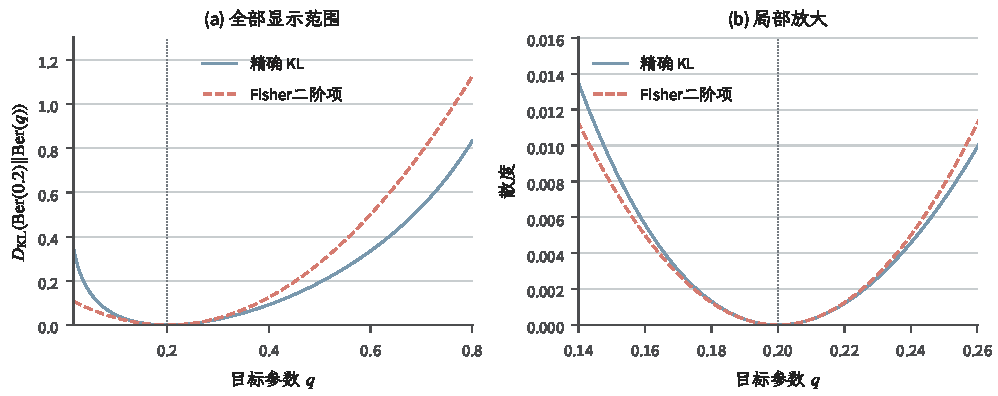
\includegraphics[width=\linewidth]{figures/01-mathematical-preliminaries/04-random-variables-distributions-and-causality/matplotlib/probability-discrete/information-fisher-local.pdf}
  \caption{Bernoulli族在\(p=0.2\)处的Fisher局部近似（解析式教学图）。
  蓝实线为\(D_{\mathrm{KL}}(P_{0.2}\Vert P_q)\)，红虚线为
  \((q-0.2)^2/[2(0.2)(0.8)]\)；右图放大邻域。图中\(0<q<1\)，
  二阶式只描述足够小的参数扰动。}
  \label{fig:information-fisher-local}
\end{figure*}

\paragraph{重参数化下的几何保持}
\label{sec:information-fisher-reparameterization}

令\(\bm\theta=\bm\theta(\bm\phi)\)为光滑局部可逆坐标变换，
Jacobian为\(\bm J=\partial\bm\theta/\partial\bm\phi\)。
在对应点\(P_{\bm\phi}=P_{\bm\theta(\bm\phi)}\)是同一张分布，
不是又施加一次统计扰动。链式法则给出
\[
  \bm s_{\bm\phi}=\bm J^\top\bm s_{\bm\theta},\qquad
  \bm F_{\bm\phi}=\bm J^\top\bm F_{\bm\theta}\bm J.
\]
因切向量满足\(\mathrm d\bm\theta=\bm J\,\mathrm d\bm\phi\)，
\[
  \mathrm d\bm\phi^\top\bm F_{\bm\phi}\mathrm d\bm\phi
  =\mathrm d\bm\theta^\top\bm F_{\bm\theta}\mathrm d\bm\theta.
\]
对同一标量目标\(L\)，梯度坐标变为
\(\bm g_{\bm\phi}=\bm J^\top\bm g_{\bm\theta}\)，
因此目标微分
\(\bm g_{\bm\phi}^\top\mathrm d\bm\phi
=\bm g_{\bm\theta}^\top\mathrm d\bm\theta\)也不变。
Fisher矩阵的数值会变，不变的是它作用于对应切向量所得到的二次型。

例如Bernoulli概率\(p\)改用logit坐标\(\phi=\log[p/(1-p)]\)，
\(\mathrm dp/\mathrm d\phi=p(1-p)\)，于是
\[
  F_\phi=\{p(1-p)\}^2F_p=p(1-p).
\]
一个坐标下的Fisher在边界附近变大，另一个变小，
但对同一分布扰动，
\((\mathrm dp)^2/[p(1-p)]=p(1-p)(\mathrm d\phi)^2\)。
坐标变换退化时不在上述局部可逆范围，例如立方高斯例子在零点的Jacobian为零。

在序贯模型中，先选对概率对象，比求逆更重要。
固定状态\(s\)，策略\(\pi_{\bm\theta}(a\mid s)\)的单步Fisher为
\[
  \bm F_s(\bm\theta)
  =\mathbb E_{A\sim\pi_{\bm\theta}(\cdot\mid s)}
    [\bm s_{\bm\theta}(s,A)\bm s_{\bm\theta}(s,A)^\top].
\]
若状态访问权重\(d(s)\)被指定并保持固定，
平均矩阵为\(\bm F_d=\mathbb E_{S\sim d}\bm F_S\)。
它衡量这一输入权重下的条件策略变化。
若把\(d_{\bm\theta}(s)\pi_{\bm\theta}(a\mid s)\)作为完整联合模型求导，
得分还包含\(\nabla\log d_{\bm\theta}(s)\)。
在正则条件下，条件策略得分均值为零，交叉项消失，联合Fisher成为
\[
  \bm F_{d_{\bm\theta}\pi_{\bm\theta}}
  =\bm F_{d_{\bm\theta}}^{\mathrm{state}}
    +\mathbb E_{d_{\bm\theta}}\bm F_S.
\]
它与把当前访问权重固定后得到的平均矩阵不是同一个对象。

第三个对象是完整轨迹Fisher。设初始分布和环境转移都不依赖参数，
参数只出现在固定有限时域\(T\)的条件动作核中。
假设共同支持和交换微分成立，各步得分二阶可积。
轨迹得分为\(\sum_{t=1}^T\bm s_t\)，其中
\(\mathbb E[\bm s_t\mid H_t]=\bm0\)，\(H_t\)为选择动作前的历史。
当\(u<t\)时，\(\bm s_u\)对\(H_t\)可测，因此
\[
  \mathbb E[\bm s_u\bm s_t^\top]
  =\mathbb E[\bm s_u\,\mathbb E(\bm s_t^\top\mid H_t)]=\bm0.
\]
展开外积便得到
\[
  \bm F_{\mathrm{trajectory}}
  =\sum_{t=1}^T\mathbb E[\bm F_{H_t}],
\]
而不是某个任意固定访问分布下的单步矩阵。
Markov策略下可把条件矩阵写成\(\bm F_{S_t}\)；
若访问权重取各时刻边缘的平均，轨迹矩阵等于对应平均矩阵的\(T\)倍。
环境或初始规律也含参数时，必须加入它们的得分，不能沿用策略独占参数的公式。

另一个常见混淆发生在样本矩阵与模型期望之间。
固定输入分布\(d\)，取条件高斯
\(Y\mid\bm X=\bm x\sim\mathcal N(\bm\theta^\top\bm x,\sigma^2)\)，
其中\(\sigma>0\)已知，\(\mathbb E_d\|\bm X\|^2<\infty\)。
同一观测的三个量为
\[
\begin{aligned}
  \bm s_{\bm\theta}(\bm x,y)
    &=\frac{y-\bm\theta^\top\bm x}{\sigma^2}\bm x,\\
  -\nabla^2_{\bm\theta}\log p_{\bm\theta}(y\mid\bm x)
    &=\frac{\bm x\bm x^\top}{\sigma^2},\\
  \bm s_{\bm\theta}\bm s_{\bm\theta}^\top
    &=\frac{(y-\bm\theta^\top\bm x)^2}{\sigma^4}\bm x\bm x^\top.
\end{aligned}
\]
按当前模型的条件分布平均时，残差平方期望为\(\sigma^2\)，
后两个矩阵的条件期望相同，再按\(d\)平均得到
\(\bm F=\mathbb E_d[\bm X\bm X^\top]/\sigma^2\)。
对一条样本，它们并不相等；残差为零时，得分外积甚至为零，
而非零输入的观测Hessian不为零。
如果真实响应规律不同于当前模型，残差平方的条件期望也可能不同，
经验得分外积的总体极限便不一定等于这个模型Fisher。
改变输入权重、使用观测Hessian或经验得分外积，都须重新说明正在近似哪个对象。

\subsubsection{局部度量下的几何更新}
\label{sec:information-geometric-update}

有了局部长度和目标微分，就可以确定在给定分布变化预算内怎样下降。
这仍是原优化任务的局部求解步骤：若参数表示有约束，应在相应可行切空间中求解，
或结合约束优化和回缩；Fisher矩阵本身不会自动保持矩与固定边缘。

\paragraph{分布变化约束下的自然梯度}
\label{sec:information-natural-gradient-update}

设目标\(L(\bm\theta)\)可微，\(\bm g=\nabla L(\bm\theta)\)，
且\(\bm F(\bm\theta)\)正定。欧氏梯度是目标微分在欧氏内积下的代表；
改用Fisher内积，代表向量也应随之改变\scite{math-amari1998natural}
\begin{definition}[自然梯度]
\label{def:information-natural-gradient}
目标\(L\)的\term{自然梯度}（natural gradient）是满足
\[
  g_{\bm\theta}(\operatorname{grad}^{F}L,\bm v)
  =\nabla L(\bm\theta)^\top\bm v
  \quad\text{对所有切向量 }\bm v
\]
的唯一向量，即
\(\operatorname{grad}^{F}L=\bm F(\bm\theta)^{-1}\nabla L(\bm\theta)\)。
\end{definition}

把目标一阶线性化，把分布KL变化二阶近似，得到局部信赖域子问题
\begin{equation}
  \min_{\bm\delta}\bm g^\top\bm\delta
  \quad\text{s.t.}\quad
  \tfrac12\bm\delta^\top\bm F(\bm\theta)\bm\delta\leq\varepsilon.
  \label{eq:information-natural-gradient-trust-region}
\end{equation}
设\(\varepsilon>0,\bm g\neq\bm0\)。
Lagrangian为
\(\bm g^\top\bm\delta+\lambda(\bm\delta^\top\bm F\bm\delta/2-\varepsilon)\)，
驻点条件给出
\(\bm g+\lambda\bm F\bm\delta=\bm0\)。
非零线性目标的最小值在椭球边界，
代入\(\bm\delta=-\lambda^{-1}\bm F^{-1}\bm g\)得到
\(\lambda=\sqrt{\bm g^\top\bm F^{-1}\bm g/(2\varepsilon)}\)，所以
\begin{equation}
  \bm\delta^\star
  =-\sqrt{\frac{2\varepsilon}{\bm g^\top\bm F^{-1}\bm g}}\,
    \bm F^{-1}\bm g.
  \label{eq:information-natural-gradient-step}
\end{equation}

可以不依赖驻点必要条件，直接验证全局最优性。
令\(\bm u=\bm F^{1/2}\bm\delta\)，约束变为
\(\|\bm u\|_2\leq\sqrt{2\varepsilon}\)，目标变为
\((\bm F^{-1/2}\bm g)^\top\bm u\)。
Cauchy--Schwarz给出
\[
  (\bm F^{-1/2}\bm g)^\top\bm u
  \geq-\|\bm F^{-1/2}\bm g\|_2\sqrt{2\varepsilon}.
\]
等号在\(\bm u\)与\(-\bm F^{-1/2}\bm g\)同向并位于球面时达到，
代回正好得到上述解。若\(\bm g=\bm0\)，一阶目标处处为零，
子问题不再选出唯一方向，应考察高阶信息或停止条件。

\begin{example}[同一分布变化预算下的两个下降方向]
\label{ex:information-natural-gradient-ellipse}
设在当前参数点，局部Fisher矩阵与目标梯度为
\[
 \bm F=\begin{pmatrix}100&0\\0&1\end{pmatrix},
 \qquad \bm g=\begin{pmatrix}1\\1\end{pmatrix}.
\]
目标的一阶变化为\(\delta_1+\delta_2\)，但同样大小的第一维位移消耗的二次KL预算
是第二维的\(100\)倍。取局部预算\(\varepsilon=0.005\)，可行椭圆为
\(100\delta_1^2+\delta_2^2\leq0.01\)。普通欧氏下降方向是\(-\bm g\)，
自然下降方向是\(-\bm F^{-1}\bm g=-(0.01,1)^\top\)。
为公平比较，把两个方向都缩放到同一椭圆边界，得到
\[
 \bm\delta_{\mathrm E}=-\frac{0.1}{\sqrt{101}}(1,1)^\top,
 \qquad
 \bm\delta_{\mathrm F}=-\frac{0.1}{\sqrt{1.01}}(0.01,1)^\top.
\]
两者都恰好消耗\(0.005\)的二次预算，目标的一阶下降量分别为
\[
 -\bm g^\top\bm\delta_{\mathrm E}
 =\frac{0.2}{\sqrt{101}}\approx0.0199,
 \qquad
 -\bm g^\top\bm\delta_{\mathrm F}
 =0.1\sqrt{1.01}\approx0.1005.
\]
自然方向减少昂贵的第一维移动，把更多预算用于第二维，因此在当前局部模型中获得
更大的下降量。这里\(\bm F\)刻画分布变化的局部代价，不是一般目标\(L\)的Hessian；
上述数值比较的是线性化目标与二次KL模型，不能直接当作真实目标的有限步下降保证。
\end{example}

图~\ref{fig:information-natural-gradient-ellipse}把两个缩放后的方向放在同一预算边界上。
两轴采用相同的物理尺度，细长椭圆说明第一维允许的位移更小。
\begin{figure}[htbp]
  \centering
  % Teaching example: F=diag(100,1), g=(1,1), epsilon=0.005.
% Both axes use 240 mm per parameter unit; the ellipse semiaxes are 0.01,0.1.
% The equal-budget endpoints are computed from the formulas in the text.
% Keep the narrow ellipse and annotate from its sides; blue/dashed/circle denotes
% Euclidean descent, red/solid/square denotes natural descent.
\begin{tikzpicture}[
  x=1mm,y=1mm,
  every node/.style={font=\figurefont\footnotesize,text=FigureInk,inner sep=1pt},
  >={Latex[length=1.5mm,width=1.1mm]}
]
  \path[use as bounding box] (0,0) rectangle (112,66);
  \coordinate (O) at (52,34);
  \coordinate (E) at ({52-24/sqrt(101)},{34-24/sqrt(101)});
  \coordinate (F) at ({52-0.24/sqrt(1.01)},{34-24/sqrt(1.01)});

  \fill[FigurePaper] (O) ellipse [x radius=2.4mm,y radius=24mm];
  \draw[FigureMuted,line width=.8pt] (O) ellipse [x radius=2.4mm,y radius=24mm];
  \draw[->,FigureStroke,line width=.6pt] (26,34)--(77,34) node[right] {\(\delta_1\)};
  \draw[->,FigureStroke,line width=.6pt] (52,6)--(52,62) node[above] {\(\delta_2\)};
  \draw[FigureStroke,line width=.6pt] (51,58)--(53,58);
  \draw[FigureStroke,line width=.6pt] (51,10)--(53,10);
  \node[anchor=west] at (56,58) {\(0.1\)};
  \node[anchor=west] at (56,7) {\(-0.1\)};
  \node[anchor=south west] at (54,35) {\(0\)};
  \node[anchor=east] at (45,49) {\(\delta_1=\pm0.01\)};
  \draw[FigureMuted,line width=.5pt] (45,46)--(49.6,34);

  \draw[->,FigureBlue,dashed,line width=1pt] (O)--(E);
  \fill[FigureBlue] (E) circle (.7mm);
  \draw[FigureBlue,line width=.6pt] (E)--(36,26)--(22,26);
  \node[anchor=east,text=FigureBlue] at (34,22) {欧氏方向\(\bm\delta_{\mathrm E}\)};

  \draw[->,FigureRed,line width=1pt] (O)--(F);
  \fill[FigureRed] ($(F)+(-.7,-.7)$) rectangle ($(F)+(.7,.7)$);
  \draw[FigureRed,line width=.6pt] (F)--(66,16);
  \node[anchor=west,text=FigureRed] at (68,16) {自然方向\(\bm\delta_{\mathrm F}\)};
\end{tikzpicture}

  \caption{局部KL预算下的下降方向（解析式教学图）。灰色椭圆满足
  \(100\delta_1^2+\delta_2^2=0.01\)，对应\(\varepsilon=0.005\)。
  蓝色虚线与圆点是缩放后的欧氏方向\(\bm\delta_{\mathrm E}\)，红色实线与方点是
  自然方向\(\bm\delta_{\mathrm F}\)；两个终点消耗相同的二次预算。
  椭圆表达分布变化代价，不是目标函数的等高线。}
  \label{fig:information-natural-gradient-ellipse}
\end{figure}

在光滑可逆重参数化下，由上一小节的矩阵和微分变换，
\[
\begin{aligned}
  \bm J\bm F_{\bm\phi}^{-1}\bm g_{\bm\phi}
  &=\bm J(\bm J^\top\bm F_{\bm\theta}\bm J)^{-1}
    \bm J^\top\bm g_{\bm\theta}\\
  &=\bm F_{\bm\theta}^{-1}\bm g_{\bm\theta}.
\end{aligned}
\]
归一化因子中的
\(\bm g_{\bm\phi}^\top\bm F_{\bm\phi}^{-1}\bm g_{\bm\phi}\)
也等于原坐标下的相应值，因此两个坐标给出同一个分布切向方向。
Bernoulli例子中，自然梯度在概率坐标为\(p(1-p)L'(p)\)，
在logit坐标为\(L'(p)\)；乘上\(\mathrm dp/\mathrm d\phi=p(1-p)\)后相同。

保持的是无穷小方向，不是任意有限离散步。
非线性坐标映射下，
\(\bm\theta(\bm\phi+\bm\delta_\phi)
=\bm\theta(\bm\phi)+\bm J\bm\delta_\phi+O(\|\bm\delta_\phi\|^2)\)，
所以分别做欧氏加法更新后的终点一般不同。
真实KL也还有\(o(\|\bm\delta\|^2)\)余项；
二次预算等于\(\varepsilon\)不保证真实KL严格不超过它。
有限步需要步长选择、真实目标或KL检查，不能由局部方向不变性直接得到全局改进。

\paragraph{奇异与近似条件下的几何更新}
\label{sec:information-singular-approximate-update}

参数冗余、退化坐标或不足的输入方向都可能使Fisher奇异。
其零空间只说明相应方向的一阶得分为零：
有时它来自完全冗余，有时如立方高斯零点，只是高阶变化未被二次型看见。
因而不能把所有零方向都理解成有限移动后分布完全不变。

回用伪逆与数值求解工具，若\(\bm g\in\operatorname{range}(\bm F)\)，
线性方程\(\bm F\bm v=\bm g\)有解，全部解为
\[
  \bm v=\bm F^\dagger\bm g+\bm z,\qquad
  \bm z\in\ker\bm F.
\]
伪逆选择当前欧氏坐标下范数最小的一个。
在得分能识别的切向商空间中，零空间分量不影响一阶分布方向，
但参数向量并不唯一，有限步的高阶效果仍可能不同。
若\(\bm g\notin\operatorname{range}(\bm F)\)，存在零方向
\(\bm z\)使\(\bm g^\top\bm z\neq0\)；
沿其下降方向任意放大仍不消耗二次预算，线性信赖域问题无下界。
此时简单写\(\bm F^\dagger\bm g\)不是原信赖域子问题的解，必须修正退化模型或约束。

阻尼使用\(\bm F+\lambda\bm I\)，其中\(\lambda>0\)，可改善病态性并保证可逆。
但它新增欧氏二次项\(\lambda\|\bm\delta\|^2\)，不是纯粹的Fisher几何：
一般坐标变化下
\[
  \bm J^\top(\bm F+\lambda\bm I)\bm J
  =\bm J^\top\bm F\bm J+\lambda\bm J^\top\bm J
  \neq\bm F_{\bm\phi}+\lambda\bm I.
\]
因此“能稳定求逆”与“保持原坐标变换性质”是不同要求。
实际计算通常求解线性系统，而不显式构造逆矩阵；
迭代容差、谱条件和矩阵近似误差也会改变得到的方向。

经验Fisher、分块或对角近似可能降低计算量，
却分别引入抽样、模型期望或跨块相关性的近似。
即使每个近似矩阵都正定，也只说明定义了某种局部内积，
不说明它等于真实分布Fisher，更不保证同样的坐标保持结论。
应区分模型下期望、真实数据下平均、固定输入权重和完整轨迹，
再说明哪一项被估计或省略。
优化收敛、模型正确性、预测校准和隐私保证还各有自己的条件；
自然梯度或KL正则不能把一种保证自动转成另一种。

\section{本章小结}
\label{sec:information-theory-statistical-geometry-summary}

开篇的编码与预测问题对应两个不同对象。
熵平均单个结果的自信息，条件熵记录已有观测后还需描述的部分；
交叉熵把预测规律放到真实规律下评价，多出的对数代价是有方向的KL。
互信息则比较联合分布与独立乘积，带噪二元例子显示观测究竟减少了多少不确定性。
连续情形必须指定参考测度，微分熵的坐标变化不能与KL的坐标不变性混为一谈。

比较两张分布时，要先说明希望看见什么差别。
总变差看到事件概率，MMD看到所选核函数类，Wasserstein看到质量移动的距离；
R\'enyi通过密度比高阶矩控制权重迁移。相同均值可以掩盖分布差异，
点质量的小位移可以保持平滑评价稳定，却使阈值事件完全改变。
因此小距离只有结合取值范围、敏感性或尾部条件，才能变成具体任务保证。
数据选择还要另付依赖代价：互信息控制平均有符号偏差，
PAC--Bayes在固定先验和参数下控制同时风险。

信息不足也给出反向限制。Le Cam与Fano要求同时构造目标分离、观测接近的候选，
自适应观测则沿实际历史累计条件信息，不能当作固定设计的独立样本。
这些结论限制任何算法能够知道什么，不等于某个算法已经达到下界。

分布优化又把比较量变成目标或约束。
Gibbs倾斜权衡收益和KL偏离，最大熵从给定矩中选择相容分布，
ELBO在表示受限的候选族中逼近后验；固定边缘的搬运问题只选择联合配对。
有限配置的负最大熵与配分函数共轭在边界仍成立，
但分布最优解不一定有有限参数表示。
最优耦合依赖紧性与成本下半连续，后验逼近依赖明确方向的支持条件。

参数化求解时，正则满秩模型的局部KL给出Fisher度量，
自然梯度据此选择同一分布切向方向。
奇异性、阻尼、矩阵近似与有限步余项都限制这一结论的直接使用。
局部几何不能替代全域散度，优化替代分布也不能替代真实数据证据。
若问题从观测规律转为干预会怎样改变结果，还需要
第~\ref{chap:causal-inference}章的生成机制与识别条件。

\chapter{因果响应}
\label{chap:causal-inference}

接受培训的人平均成绩更高，是培训提高了成绩，还是基础较好的人更愿意参加培训？
第~\ref{chap:random-variables}章已经建立条件分布与统计推断，第
~\ref{chap:information-theory-and-statistical-geometry}章进一步比较分布及其对任务的
影响。但把成绩预测得很准，仍不能回答主动安排培训以后会发生什么。后一个问题要求
说明：改变的究竟是对已有记录的筛选，还是产生记录的机制。

本章研究因果响应及生成它的结构。响应把行动与个体背景映射为结果；生成结构进一步
说明这个整体映射由哪些局部关系和机制合成。我们以处理\(T\)、结果\(Y\)与处理前
信息\(X\)为共同例子，区分给定模型的计算、数据对响应的识别，以及数据对生成结构的
推断。模型明确给定时，可以直接比较行动，也可以在得知某人的事实以后计算替代结果；
这不意味着数据已经证明该模型正确。反过来，有些平均响应可以由实验设计识别，而无须
唯一恢复每一个局部方程。

阅读上先把响应当作可使用的数学对象，明确输入、行动规则和背景分布，再分别比较个体、
总体及局部变化。事实证据只更新对背景的认识，替代行动则改变响应映射。识别部分检查
数据能否支持这些答案，结构部分才打开模型内部，证明无环局部机制怎样实现前面使用的
映射，并建立本章所需的图语义。这样可以始终区分“在模型内算得出”与“由资料确定得了”。

\section{因果响应的表示}
\label{sec:causal-response-representation}

要询问一个人接受培训后的成绩，至少需要说明培训方案、这个人的背景、成绩测量时间，
以及安排培训会改变哪些生成规则。只给出一个拟合函数
\(\mathbb E[Y\mid T=t,X=x]\)还不够：它描述自然分配下的条件平均，未必描述主动安排
培训的后果。本节先规定能够回答行动问题的最低模型接口，暂不要求把全部内部结构画成图。

\subsection{原因与背景的响应表示}
\label{sec:causal-observation-generation}

用\(t\)表示可以设定的处理值，用\(\bm u\)表示在所比较行动之间保持的个体背景。
背景包含模型没有继续解释的差异，例如既有能力和未测量的环境因素；它与“所有已观测
协变量”不是同义词。模型\(M\)规定背景的联合分布、自然运行规则和允许的行动。
本节假定这些规则已经给出唯一结果，后面再说明怎样从局部方程保证这一点。

\begin{definition}[因果响应与自然、行动映射]
  \label{def:causal-response-interface}
  给定背景可测空间\((\mathcal U,\mathscr U)\)及概率测度\(P_{\bm U}\)，
  自然变量的可测状态空间\(\mathcal V\)，处理空间\(\mathcal T\)和结果空间
  \(\mathcal Y\)。固定模型\(M\)提供唯一值的可测自然映射
  \(F_M:\mathcal U\to\mathcal V\)，以及每个允许行动\(a\)的唯一值可测映射
  \(F_M^a:\mathcal U\to\mathcal V\)。后者由模型指定的机制替换产生，而非任意另选函数。
  若\(a(t)\)表示把处理设为\(t\)的允许行动，\(\pi_Y\)表示取结果坐标，则
  \term{因果响应}（causal response）是映射
  \begin{equation}
    R_M:\mathcal T\times\mathcal U\longrightarrow\mathcal Y,
    \qquad
    R_M(t,\bm u)=\pi_Y\bigl(F_M^{a(t)}(\bm u)\bigr).
    \label{eq:causal-response-interface}
  \end{equation}
  本章要求\(R_M\)对乘积可测结构可测。自然变量为
  \(\bm V=F_M(\bm U)\)，行动后的变量为\(\bm V_a=F_M^a(\bm U)\)。
\end{definition}

固定\(\bm u\)时，\(t\mapsto R_M(t,\bm u)\)回答同一单位怎样响应不同处理；
让\(\bm U\)按\(P_{\bm U}\)变化，才得到总体响应分布。外生背景的各分量可以相关，
定义没有默许独立性。若采用有限维参数表示\(M_{\bm\theta}\)，参数
\(\bm\theta\)描述研究者选定的机制；修改拟合参数是在改变模型，设置\(t\)则是在一个
固定模型内行动。两种变化不能互相代替。

下面用两套二元机制计算这一区别。设背景满足
\[
  U\sim\operatorname{Bernoulli}(1/2).
\]
处理与结果均取\(0,1\)。模型甲为
\begin{equation}
  T=U,\qquad Y=U;
  \label{eq:causal-observational-equivalence-confounding}
\end{equation}
模型乙为
\begin{equation}
  T=U,\qquad Y=T.
  \label{eq:causal-observational-equivalence-effect}
\end{equation}
两者自然映射都是\(F_M(u)=(u,u)\)，从而
\[
  \begin{aligned}
    \mathbb P(T=0,Y=0)&=\mathbb P(T=1,Y=1)=\frac12,\\
    \mathbb P(T=0,Y=1)&=\mathbb P(T=1,Y=0)=0.
  \end{aligned}
\]
在甲中，处理不进入结果规则；在乙中，结果直接复制处理。若允许的行动是把处理规则
替换为常数\(t\)，保留结果规则，则
\[
  F_{M_{\text{甲}}}^{a(t)}(u)=(t,u),\qquad
  F_{M_{\text{乙}}}^{a(t)}(u)=(t,t),
\]
所以\(R_{M_{\text{甲}}}(t,u)=u\)，而
\(R_{M_{\text{乙}}}(t,u)=t\)。两模型的自然映射相同，行动映射不同；
观测记录无法仅凭样本量区分这种差异。

\subsection{机制干预下的潜在结果}
\label{sec:causal-intervention-potential-outcomes}

上例没有筛出自然接受处理的人，而是改变了处理怎样产生。这就是机制干预：
指定一项生成规则的替换，再让其余规则根据新的输入继续运行。行动的因果含义来自
这种替换约定，不来自函数名称或概率记号。

\begin{definition}[理想干预]
  \label{def:causal-intervention}
  对给定模型的处理变量\(T\)作\term{干预}（intervention）
  \(\operatorname{do}(T=t)\)，表示删除自然生成\(T\)的规则，并以常量规则
  \(T=t\)替换。其余生成规则和指定的背景分布\(P_{\bm U}\)保持不变。
  由行动映射\(F_M^{a(t)}\)推前得到的分布记作
  \(P^{\operatorname{do}(T=t)}\)。
\end{definition}

“其余规则不变”不是说其余变量的取值不变。若培训改变技能，技能再影响成绩，
行动后技能和成绩都应重算。只锁住所有非处理字段再评估一个预测器，通常不是这一行动。
多变量行动同样由\(F_M^a\)表达，但模型必须说明哪些规则替换、哪些保留。

\begin{definition}[潜在结果]
  \label{def:causal-potential-outcomes}
  对明确的目标总体、处理版本和结果测量时间，\term{潜在结果}
  （potential outcome）是随机变量
  \begin{equation}
    Y(t)=R_M(t,\bm U).
    \label{eq:causal-response-potential-outcome}
  \end{equation}
  对二元处理，\((Y(0),Y(1))\)定义在同一背景概率空间上；两项分别表示同一单位
  在两种处理下的结果，而不是分别抽取两个人。
\end{definition}

可测性保证可以讨论潜在结果的概率规律。记\(\mathcal L(Z)\)为随机变量\(Z\)的分布，
则
\[
  \mathcal L(Y(t))
  =
  (R_M(t,\cdot))_{\#}P_{\bm U}
  =
  \mathcal L(Y\mid\operatorname{do}(T=t)).
\]
符号\(\#\)表示第~\ref{sec:rv-pushforward}节的分布推前。这里的
\(\operatorname{do}\)标记修改后的模型，不是对自然事件\(T=t\)作普通条件化。
潜在结果聚焦所选行动下的输出；仅有一张潜在结果表，并不自动给出其他变量的完整
生成机制\scite{math-hernan2020whatif}

观察条件分布\(p(y\mid T=t)\)会筛选自然规则恰好给出处理\(t\)的单位，因而同时
包含处理作用和进入处理组的选择。在上面两套机制中，都有
\[
  \mathbb P(Y=1\mid T=1)=1,\qquad
  \mathbb P(Y=1\mid T=0)=0.
\]
但对甲，设定处理以后结果仍为\(U\)，故
\[
  \mathbb P(Y=1\mid\operatorname{do}(T=t))=\frac12,
  \qquad t\in\{0,1\};
\]
对乙，设定处理以后结果为\(t\)，故
\[
  \mathbb P(Y=1\mid\operatorname{do}(T=t))=t.
\]
相同的观测关联对应不同的行动后果。缺少的是关于响应机制的约束，不是更精确地估计
已经相同的两个条件概率。

固定处理值并非唯一行动。\term{随机干预}（stochastic intervention）用新的随机
规则替换处理规则，例如给定处理前信息\(X=x\)时，按\(q(t\mid x)\)安排培训。
一种明确构造是加入独立于原背景的随机量\(W\)，指定
\(T=g_q(X,W)\)，使其条件分布为\(q(\cdot\mid X)\)，再运行保留的机制。
确定性策略是新规则不再需要随机化的特例。随机化是否独立、行动可使用哪些信息，
都是干预定义的一部分；仅把某个概率因子改写为\(q\)不能保证其余现实机制未变。
局部机制成立时相应的分解公式在第~\ref{sec:causal-mechanism-composition}节建立。

\subsection{观测结果与干预响应的连接}
\label{sec:causal-response-observation-link}

潜在结果已经定义，还需要说明实际记录对应其中哪一项。目标总体规定对谁平均，
处理版本规定怎样行动，测量时间规定观察何种结果。若这些口径未固定，同一个
“接受培训”可能混合不同课程与时长，\(Y(1)\)就未必是一个确定的对象。

\begin{definition}[处理一致性与无干扰]
  \label{def:causal-consistency-no-interference}
  对明确的处理版本，\term{一致性}（consistency）要求实际处理对应的结果满足
  \(Y=Y(T)\)几乎必然成立；特别地，
  \begin{equation}
    \begin{gathered}
      T=t\Longrightarrow Y=Y(t),\\
      \text{二元处理时，}\quad Y=TY(1)+(1-T)Y(0).
    \end{gathered}
    \label{eq:causal-consistency}
  \end{equation}
  对\(n\)个单位，无干扰要求：每个\(i\)及任意两个处理向量
  \(\bm t,\bm t'\)，只要\(t_i=t_i'\)，就有
  \(Y_i(\bm t)=Y_i(\bm t')\)几乎必然成立。因此单位\(i\)的潜在结果才可简记为
  \(Y_i(t_i)\)。
\end{definition}

一致性连接自然记录与行动响应，没有把未采取行动的结果变成可见记录。若模型给出
自然处理\(T=F_{M,T}(\bm U)\)，这一条件要求自然结果与
\(R_M(F_{M,T}(\bm U),\bm U)\)相合；不能任意拼接不相容的自然函数与响应族。
在依规则替换而构造的无环模型中，这种相合性可以逐方程检查。

无干扰则限制研究单位之间的相互作用。疫苗接种、社交网络和市场竞争中，一人的行动
可能改变他人的暴露或机会；此时\(Y_i(\bm t)\)往往依赖整个处理向量。
例如\(Y_i(\bm t)=t_i+\eta\sum_{j\ne i}t_j/(n-1)\)在
\(n>1,\eta\ne0\)时不满足无干扰。可以另行规定网络暴露、分组方案或总体处理比例，
但不能继续把只比较\(t_i\)的效应解释为所有联动后果。

通常所说的稳定单位处理值假设把处理版本唯一性和无干扰合在一起。它们与分配机制仍
须分开判断：分配机制规定\(T\)怎样依赖\(X,Y(0),Y(1)\)等量，一致性只连接实际
处理与观察结果。即使处理版本清楚且单位互不干扰，主动选择培训的人也可能具有不同
背景。响应的表示到此已建立，能否由这种选择后的观测恢复响应，是后面识别部分的问题。

\section{因果响应的比较与变化}
\label{sec:causal-response-comparison}

同一项培训可以提高平均成绩，却使一部分人的成绩下降；它也可能不改变均值，只减少
低分结果。因而“有没有效”必须落实为具体比较。本节固定模型、目标总体和处理版本，
分别比较同一背景的两个结果、背景总体的平均与分布，以及连续剂量的局部变化。

\subsection{同一背景下的响应比较}
\label{sec:causal-individual-response}

\begin{definition}[同一背景下的响应差]
  \label{def:causal-individual-effect}
  对实值结果及允许的处理值\(t,t'\)，固定背景\(\bm u\)的响应差定义为
  \begin{equation}
    \Delta_M(t,t';\bm u)=R_M(t,\bm u)-R_M(t',\bm u).
    \label{eq:causal-individual-response-difference}
  \end{equation}
  二元处理的\term{个体处理效应}（individual treatment effect）是随机变量
  \(Y(1)-Y(0)=\Delta_M(1,0;\bm U)\)。
\end{definition}

这里的减法保持同一背景，而不是用一个处理组成员减去另一个未处理组成员。
例如\(R_M(t,u)=u+(2u-1)t\)，其中\(u\in\{0,1\}\)。对背景\(u=1\)，处理使
结果增加\(1\)；对\(u=0\)，处理使结果减少\(1\)。比较两名不同背景个体的实际
结果，还混入了基础值\(u\)的差异。

给定模型和背景时，两个响应都可以计算。但每个单位的实际记录只能包含
\(Y(T)\)，不会同时包含同一时刻的\(Y(1)\)与\(Y(0)\)。因此“个体效应有明确定义”
与“它能由该人的一次观察确定”是两件事。即使已知某人当前结果为零，仍需要机制或
关于背景的信息才能计算另一行动下的结果。

对向量结果，可以先报告各坐标差，也可以指定具有实质含义的效用函数
\(h:\mathcal Y\to\mathbb R\)，比较
\(h(R_M(t,\bm u))-h(R_M(t',\bm u))\)。对类别结果，直接相减通常没有意义，
可以比较某事件的指示量。选择\(h\)是在规定目标，不是纯粹的记号替换：
提高收入、降低风险和同时满足两项要求，可能给出不同的行动排序。

\subsection{背景总体下的响应比较}
\label{sec:causal-population-response}

实践中很少能逐人确定背景。总体比较把背景按同一个目标分布聚合，回答这套行动对
指定人群的后果。聚合可以保留一个均值，也可以保留完整结果分布；它们丢失的信息不同。

\subsubsection{总体与条件总体的平均响应比较}
\label{sec:causal-average-response}

\begin{definition}[平均处理效应]
  \label{def:causal-average-treatment-effect}
  对二元处理，假设\(Y(0),Y(1)\)都可积，\term{平均处理效应}
  （average treatment effect, ATE）定义为
  \begin{equation}
    \tau
    =
    \mathbb E[Y\mid\operatorname{do}(T=1)]
    -
    \mathbb E[Y\mid\operatorname{do}(T=0)].
    \label{eq:causal-ate-interventional}
  \end{equation}
\end{definition}

两个干预总体使用同一个\(P_{\bm U}\)。由潜在结果与干预分布的对应关系及期望线性性，
\begin{equation}
  \tau
  =\mathbb E[Y(1)-Y(0)]
  =\mathbb E[Y(1)]-\mathbb E[Y(0)].
  \label{eq:causal-ate-potential-outcomes}
\end{equation}
可积性排除了\(\infty-\infty\)这样的未定义运算。线性期望说明计算平均差只需要两个
边缘均值，并没有使同一单位的两个结果同时可见。上例若
\(\mathbb P(U=1)=\mathbb P(U=0)=1/2\)，ATE为零，但没有人的个体效应为零。

若要辨认哪些人可能受益，可以在处理前协变量\(X\)下分层。
\begin{definition}[条件平均处理效应]
  \label{def:causal-conditional-average-effect}
  设\(X\)在所比较干预下保持同一取值与含义，且两种潜在结果可积。
  \term{条件平均处理效应}（conditional average treatment effect, CATE）是
  \begin{equation}
    \tau(x)=\mathbb E[Y(1)-Y(0)\mid X=x],
    \qquad P_X\text{几乎处处}.
    \label{eq:causal-cate}
  \end{equation}
\end{definition}
它对具有相同已知特征的人平均，不等于这些人逐个具有相同效应。取
\(X=U\)时，上例的\(\tau(1)=1,\tau(0)=-1\)；若\(X\)未包含\(U\)，
条件平均仍可能掩盖层内差异。不能把处理后的技能水平直接当作这里不随行动变化的
\(X\)：按两种行动各自产生的技能筛人，通常不是比较同一条件总体。

全期望给出\(\tau=\mathbb E_X[\tau(X)]\)。若响应机制不变而目标总体从\(P_X\)
换为\(Q_X\)，且对应的条件背景规律与条件效应保持不变，新ATE为
\(\int\tau(x)Q_X(\mathrm dx)\)。这是人群权重的变化，不是机制突然发生改变；
条件效应能否跨总体保留本身仍需假设。目标总体、处理版本或测量时间改变，都应重新
标明效应的含义。

对有限处理集合\(\mathcal T\)，同样定义
\[
  \tau(t,t')=\mathbb E[Y(t)-Y(t')].
\]
若行动由处理前信息决定，则要比较整个策略。令有限动作集合为\(\mathcal A\)，
策略\(\pi(a\mid x)\)用独立的新增随机化，在给定\(X=x\)时选择动作\(a\)。
在所有潜在结果可积时，它的单步价值为
\begin{equation}
  V(\pi)=\mathbb E_X\left[
    \sum_{a\in\mathcal A}\pi(a\mid X)\mathbb E[Y(a)\mid X]
  \right].
  \label{eq:causal-policy-value}
\end{equation}
式中独立随机化保证选择动作不会额外按未观测背景筛人。确定性策略是
\(\pi\)集中于一个动作的特例。这里定义的是给定模型内的目标；多值处理需要哪些
观测覆盖、策略可使用哪些已有记录，在第~\ref{sec:causal-effect-identification}节
再检查。连续剂量也不能被当作每个精确值都具有正概率的离散组。

\subsubsection{干预结果的分布响应比较}
\label{sec:causal-distribution-response}

平均值只记录分布的一个特征。设\(U\)等概率取\(-1,1\)，
\(Y(0)=0,Y(1)=U\)，则ATE为零，但处理后从人人得到零变成两种相反结果。
若低于零代表失败，这种变化对决策显然重要。

对实值结果，定义干预分布函数与其广义分位数
\[
  F_t(y)=\mathbb P(Y(t)\leq y),\qquad
  Q_t(p)=\inf\{y:F_t(y)\geq p\},\quad 0<p<1.
\]
\(F_t(y)-F_{t'}(y)\)比较低于阈值的概率，\(Q_t(p)-Q_{t'}(p)\)比较两个总体
处于同一分位位置的结果。后者并不是个体效应
\(Y(t)-Y(t')\)的第\(p\)分位数，因为处于两个分布相同排名的未必是同一个人。
只有额外规定跨行动的排序对应关系，才能把这种配对解释成个体变化。

也可以使用第~\ref{chap:information-theory-and-statistical-geometry}章的分布比较
尺度。总变差比较事件概率而不要求矩；采用\(p\)阶Wasserstein距离时应满足所用
空间和有限\(p\)阶矩条件；使用KL散度则须检查绝对连续性及其值是否有限。
尺度的选择服务于所关心的风险或损失，不能用一个小均值差代替所有分布都接近。

两个干预边缘即使完全已知，仍没有说明它们如何在同一背景上配对。
第~\ref{sec:causal-factual-counterfactual}节将用两张联合表说明：分布比较足以回答
部分总体问题，却不足以回答已知某人事实结果后的替代结果。

\subsection{连续处理下的局部响应变化}
\label{sec:causal-local-response}

二元处理适合比较有无行动；连续剂量还可以询问“在当前剂量附近再增加一点会怎样”。
这时回用第~\ref{sec:analysis-derivatives-linear-approximation}节的局部线性近似，
但求导对象必须是固定模型、固定背景下的响应。

\begin{definition}[局部响应导数]
  \label{def:causal-local-response}
  设处理取值位于开集\(\mathcal T\subseteq\mathbb R^k\)，结果位于
  \(\mathbb R^m\)。用粗体标明向量剂量；若
  \(\bm t\mapsto R_M(\bm t,\bm u)\)在\(\bm t_0\)可微，其局部响应
  Jacobian为\(D_{\bm t}R_M(\bm t_0,\bm u)\)，满足
  \[
    R_M(\bm t_0+\bm h,\bm u)-R_M(\bm t_0,\bm u)
    =D_{\bm t}R_M(\bm t_0,\bm u)\bm h+o(\|\bm h\|).
  \]
  标量处理、标量结果时记为\(\partial_tR_M(t_0,\bm u)\)。
\end{definition}

该导数是每单位剂量的局部变化，不是任意有限剂量差。比如
\(R_M(t,u)=u+t^2\)，从\(t=1\)增加到\(1+h\)的响应差是\(2h+h^2\)，
局部导数为\(2\)。\(h\)很小时一阶项有用，但从\(1\)变到\(2\)的差为\(3\)，
不能直接用导数值\(2\)代替。离散行动没有这样的邻域，仍应使用有限差。

总体平均响应\(m(t)=\mathbb E[R_M(t,\bm U)]\)还包含积分，不能仅凭每个人的
响应可微就交换求导与期望。下面给出一个可以直接检查的充分条件。
\begin{theorem}[平均响应的求导]
  \label{thm:causal-response-differentiation}
  设\(I\)是包含\(t_0\)的开区间，\(R_M(t_0,\bm U)\)可积。若对几乎每个
  \(\bm u\)，\(R_M(\cdot,\bm u)\)在\(I\)可微，且存在非负可积函数
  \(g(\bm U)\)，使
  \[
    |\partial_tR_M(t,\bm u)|\leq g(\bm u),
    \qquad t\in I,
  \]
  则\(m\)在\(t_0\)可微，且
  \begin{equation}
    m'(t_0)=\mathbb E[\partial_tR_M(t_0,\bm U)].
    \label{eq:causal-average-response-derivative}
  \end{equation}
\end{theorem}
\begin{proof}
  对足够小的非零\(h\)，中值定理给出
  \[
    \left|
      \frac{R_M(t_0+h,\bm u)-R_M(t_0,\bm u)}{h}
    \right|\leq g(\bm u).
  \]
  因而\(R_M(t_0+h,\bm U)\)可积，且差商几乎处处收敛到
  \(\partial_tR_M(t_0,\bm U)\)。可积的\(g\)统一控制这些差商，支配收敛定理
  允许将极限移入期望，得到
  \[
    \lim_{h\to0}\frac{m(t_0+h)-m(t_0)}{h}
    =
    \mathbb E\!\left[
      \lim_{h\to0}
      \frac{R_M(t_0+h,\bm U)-R_M(t_0,\bm U)}{h}
    \right],
  \]
  即所述结论。
\end{proof}

向量处理可以在相应可积控制下逐坐标求导；若要得到完整可微性，则需足以控制
Jacobian及余项的邻域条件。上述定理把“个体可微”与“可交换积分”分开，
后者限制少量背景下异常陡峭的响应，避免其破坏总体极限。

局部因果导数也不等于观测回归斜率
\(\partial_t\mathbb E[Y\mid T=t,X=x]\)。后者随\(t\)改变的还可能是自然进入
该剂量的人群；第~\ref{sec:causal-sensitivity-ranges}节将明确计算这种偏差。
它同样不同于随机轨道的It\^o微分：这里对可设定输入作普通局部变化，背景固定；
随机轨道微分描述随时间累积的随机变化，一般不存在普通逐轨道时间导数。
因此模型的光滑性支持局部计算，却不同时保证这个导数能由观测识别或能外推到大幅行动。

\section{给定事实后的因果响应}
\label{sec:causal-counterfactual-recourse}

总体比较按目标背景分布平均；若已知某人的成绩、处理和其他事实，这些信息应当参与
计算。例如，对刚得到不利决策的人，问题不是“随机抽一个人接受培训会怎样”，而是
“已知这个人的记录，培训能否改变他的决策”。本节仍固定模型，只用事实更新对背景
的认识，再在同一背景上比较替代行动。

\subsection{事实条件下的反事实计算}
\label{sec:causal-factual-counterfactual}

\begin{definition}[给定响应模型的反事实变量]
  \label{def:causal-counterfactual}
  设模型\(M\)具有定义~\ref{def:causal-response-interface}的自然映射\(F_M\)及
  行动映射\(F_M^a\)。在同一外生背景\(\bm U\)上，\term{反事实}
  （counterfactual）变量定义为\(\bm V_a=F_M^a(\bm U)\)。
  给定实际证据\(\bm E\)后的反事实分布是\(\bm V_a\)关于该证据的条件分布，
  而不是重新按背景总体抽取一个人。
\end{definition}

事实证据可来自自然变量的一部分，也可包括带噪测量；后一情形把测量随机性一并纳入
背景，使证据的生成规则明确。反事实计算通常称为“溯因、干预、预测”：
溯因由事实得到背景条件分布，干预切换到允许的行动映射，预测将同一个背景条件分布
推到结果空间。这里的溯因是给定模型内的条件化，并不是由一条记录证明模型正确。

设空间允许选取正则条件分布
\(P_{\bm U\mid\bm E=\bm e}\)，例如本章常用的标准Borel空间。回用第
~\ref{sec:rv-conditional-distribution}节，对任意可测集合\(B\)，三步合成为
\begin{equation}
  \begin{aligned}
    \mathbb P(\bm V_a\in B\mid\bm E=\bm e)
    &=
    \bigl((F_M^a)_{\#}
      P_{\bm U\mid\bm E=\bm e}\bigr)(B)\\
    &=
    \int\mathbb I\{F_M^a(\bm u)\in B\}
      P_{\bm U\mid\bm E=\bm e}(\mathrm d\bm u).
  \end{aligned}
  \label{eq:causal-counterfactual-pushforward}
\end{equation}
式中事实只进入背景条件分布，行动只进入映射。连续证据点通常概率为零，等式按所选
正则条件分布版本理解，只保证对证据分布几乎处处的\(\bm e\)成立。在一个指定的
零概率证据点上报告数值，还需要选定版本或连续性等额外结构；积分恒等式本身不能
唯一规定每个点的条件值。

考虑已经明确给定的教学模型
\begin{equation}
  X=U_X,\qquad
  T=f_T(X,U_T),\qquad
  Y=2X+3T+U_Y.
  \label{eq:causal-counterfactual-linear-example}
\end{equation}
它直接提供自然映射及替换处理规则后的映射。某人的事实为
\(X=2,T=0,Y=5\)，于是
\[
  U_Y=5-2\times2-3\times0=1.
\]
保持该人的\(X,U_Y\)不变，把处理设为\(1\)，得到
\[
  Y_{T\leftarrow1}=2\times2+3\times1+1=8.
\]
差值\(3\)来自给定结果规则中的处理作用。事实不必确定全部背景，例如可能仍不知道
\(U_T\)；只要未确定部分不影响本次行动后的结果，仍能得到这个点值。
若结果规则不确定，或未确定的背景继续进入结果，则应给出条件分布或范围。

\begin{example}[两点背景后验的反事实推前]
  \label{ex:causal-two-point-background-posterior}
  令背景类型\(U\in\{u_{\mathrm L},u_{\mathrm H}\}\)先验概率各为\(1/2\)。
  事实中观察到二元信号\(S=1\)，且模型规定
  \[
    \mathbb P(S=1\mid U=u_{\mathrm H})=\frac34,\qquad
    \mathbb P(S=1\mid U=u_{\mathrm L})=\frac14.
  \]
  因而\(\mathbb P(S=1)=\frac12(\frac34+\frac14)=\frac12\)，Bayes公式给出
  \[
    \mathbb P(U=u_{\mathrm H}\mid S=1)=\frac34,\qquad
    \mathbb P(U=u_{\mathrm L}\mid S=1)=\frac14.
  \]
  若行动\(a\)下的结果在两类背景中分别为
  \(F_{M,Y}^a(u_{\mathrm L})=2,F_{M,Y}^a(u_{\mathrm H})=6\)，则
  \[
    \mathcal L(Y_a\mid S=1)=\frac14\delta_2+\frac34\delta_6,\qquad
    \mathbb E[Y_a\mid S=1]=\frac14\,2+\frac34\,6=5.
  \]
  忽略事实而按先验重新抽取背景，得到总体干预分布
  \(\frac12\delta_2+\frac12\delta_6\)，均值为\(4\)。
  两个答案使用同一行动映射，只是反事实计算保留了事实提供的背景信息。
\end{example}

这个例子也可放回完整背景接口：另加独立测量随机量生成信号\(S\)，行动结果只依赖
类型\(U\)，于是积分掉测量背景就得到上面的两点后验。未知背景不必被硬选成某一类。

还有一种更深的歧义：即使知道两种行动各自的总体分布，也未必知道同一个人的两个
结果怎样配对。设两种干预结果均为\(\operatorname{Bernoulli}(1/2)\)。
模型甲令一半单位满足\((Y(0),Y(1))=(0,0)\)，另一半满足\((1,1)\)；
模型乙令两类单位分别满足\((0,1)\)和\((1,0)\)。甲的个体效应恒为零，
乙的个体效应等概率取\(1,-1\)，而两模型的ATE都为零。

图~\ref{fig:causal-cross-world-couplings}给出了对应的联合概率表。用定义
~\ref{def:information-coupling}的语言，两者是相同边缘的不同耦合。
已知\(Y(0)=0\)时，甲给\(Y(1)=0\)，乙给\(Y(1)=1\)。在独立随机分配处理
的事实世界里，观察到\(T=0,Y=0\)就能形成这项对照：两个模型仍给出不同反事实。

\begin{figure}[htbp]
  \centering
  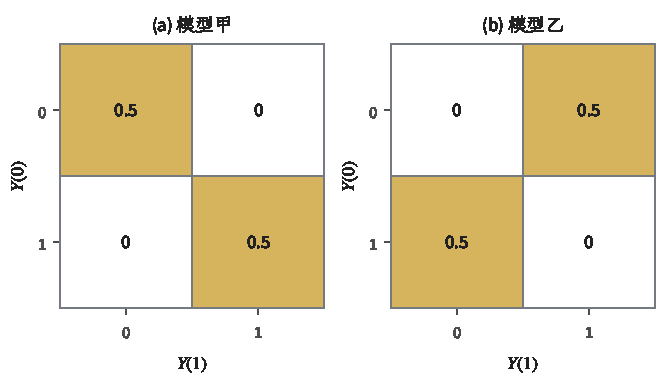
\includegraphics[width=\linewidth]{figures/01-mathematical-preliminaries/04-random-variables-distributions-and-causality/matplotlib/concepts-probability/causal-cross-world-couplings.pdf}
  \caption{相同干预边缘的两种跨世界配对。行对应\(Y(0)\)，列对应\(Y(1)\)，格内
  数字为联合概率；每张表的行和、列和均为\(1/2\)。甲的个体效应恒为零，乙的个体
  效应等概率取\(1,-1\)，两者ATE均为零。这是相容机制的教学构造，不是随机试验
  直接观察到的潜在结果联合表。}
  \label{fig:causal-cross-world-couplings}
\end{figure}

两套配对连完整随机试验的两组边缘也无法区分。要回答条件个体反事实，还需要关于
跨世界联合结构的机制限制，或具有适当稳定性、时间和携带效应假设的重复干预资料；
否则应保留相容范围。模型明确给定时可以用式
~\eqref{eq:causal-counterfactual-pushforward}计算，数据是否足以确定这套模型则是
第~\ref{sec:causal-effect-identification}节的另一个问题。

\subsection{目标约束下的行动补救}
\label{sec:causal-action-recourse}

反事实计算还可以反过来服务于行动选择：怎样以尽量低的代价，让同一个人的决策
达到目标？先区分两种看似相近的操作。对预测器\(\widehat y=f(x,t)\)，输入替换给出
\[
  f(x,1)-f(x,0).
\]
这只是已训练函数对字段变化的响应。若现实培训提高技能、同时占用工作时间，那么
只改“是否培训”一列而锁住技能和时间，通常不是任何可实施的行动结果。

\begin{definition}[因果行动补救]
  \label{def:causal-recourse}
  给定事实证据、可实施行动集合\(\mathcal A(x)\)、响应模型、行动成本\(c(a;x)\)
  与目标决策集合\(G\)，\term{行动补救}（algorithmic recourse）寻找能够使行动后
  的决策落入\(G\)的可行行动。因果行动补救用同一背景下的干预状态
  \(\bm V_a=F_M^a(\bm U)\)评价成功条件，并按机制重算所有受行动影响的状态。
\end{definition}

令\(d\)为最终决策规则。若事实唯一确定背景\(\bm u\)，优化形式为
\begin{equation}
  \min_{a\in\mathcal A(x)}c(a;x)
  \quad\text{使得}\quad d(F_M^a(\bm u))\in G.
  \label{eq:causal-recourse-objective}
\end{equation}
可行集合规定实际允许做什么，成本规定如何比较行动，成功约束规定要得到何种决策。
它们对应第~\ref{chap:optimization}章的约束优化接口，但不能只根据一个距离函数
代替全部三项。低输入距离不等于低行动成本；不可改变属性也不应成为行动建议。
若可行集合为空，应报告无法在当前约束下补救，而不是输出一个不可执行的最近点。

多数事实只能给出背景条件分布。给定可容许失败概率\(\alpha\in[0,1]\)，可以采用
概率型约束
\begin{equation}
  \mathbb P\bigl(d(F_M^a(\bm U))\in G\mid\bm E=\bm e\bigr)
  \geq1-\alpha.
  \label{eq:causal-recourse-probability}
\end{equation}
若背景空间带有指定拓扑，可选所用条件分布版本的支持
\[
  \mathcal S_{\bm e}
  =\operatorname{supp}P_{\bm U\mid\bm E=\bm e}.
\]
要求
\begin{equation}
  d(F_M^a(\bm u))\in G,\qquad \bm u\in\mathcal S_{\bm e},
  \label{eq:causal-recourse-robust}
\end{equation}
得到支持上的最坏情形保证。一般可测空间没有默认的拓扑支持，此时应明确给出候选
背景集合，而不是含糊使用“所有可能背景”。支持上逐点成功通常强于概率一成功，
因为它还涉及零概率点上的模型取值。

两点后验例子可以直接比较这些条件。若目标是\(Y_a\geq5\)，行动\(a\)的后验成功
概率为\(3/4\)，因此在\(\alpha=1/4\)时满足概率约束；但低类型背景的结果为\(2\)，
不能满足支持上的最坏情形保证。只挑高类型作为“代表背景”会漏掉这项风险。

补救也有时间和多人联动的边界。许多人同时接受建议可能改变价格、名额或审核规则；
决策系统更新后，原建议未必仍有效；资源竞争也可能使原先逐人可行的行动无法共同
执行。因此当前模型中存在一个成功行动，不等于建议已经通过现实可行性、持久性
或公平性验证。

\subsection{目标属性干预下的公平补救}
\label{sec:causal-fair-recourse}

达到有利决策与公平是两项要求。一个行动可能只在事实属性下成功，却在同一人的
替代属性世界里失败。要讨论这种差别，必须先说明哪些属性影响应当被排除，以及
替代属性在模型中如何改变其他状态。

令受保护属性为\(A\)，事实证据为\((X=x,A=a)\)。本小节的\(X\)泛指用于推断
背景的其他事实，可能包含属性的后继变量；它不再具有CATE中“处理前且保持不变”
的自动含义。事实中给定\(X=x\)，并不要求替代属性世界的\(X\)仍等于\(x\)。
\begin{definition}[反事实公平]
  \label{def:causal-counterfactual-fairness}
  在给定响应模型与预测规则下，\term{反事实公平}（counterfactual fairness）
  要求：对每个允许的替代属性\(a'\)和每个可测预测值集合\(B\)，以下等式对事实
  证据分布几乎处处的\((x,a)\)成立：
  \begin{equation}
    \begin{aligned}
      &\mathbb P(\widehat Y_{A\leftarrow a}\in B\mid X=x,A=a)\\
      &\qquad=
      \mathbb P(\widehat Y_{A\leftarrow a'}\in B\mid X=x,A=a).
    \end{aligned}
    \label{eq:causal-counterfactual-fairness}
  \end{equation}
  两个属性世界均使用同一个事实背景条件分布，并重新计算由属性影响的状态及预测。
\end{definition}

等式右侧仍以事实\(A=a\)为条件，而不是改用另一群人的证据\(A=a'\)。
只在输入表中替换\(A\)并固定其全部后继变量，检验的是另一个对象。属性干预在这里
是明确模型下的比较操作，也不表示应建议个人改变该属性。

把公平条件加入补救时，为避免与属性值混淆，记补救行动为\(b\)。
要求模型已经规定联合行动映射\(F_M^{b,A\leftarrow a'}\)：对每个属性世界，
保留同一个可比较的行动\(b\)，不对该世界偷偷重新选择更有利的行动。行动与属性
替换须互相兼容，且所比较世界中行动的可实施含义应明确。定义
\[
  \Pi_b^{a'}(B;x,a)
  =
  \mathbb P\bigl(
    d(F_M^{b,A\leftarrow a'}(\bm U))\in B
    \mid X=x,A=a
  \bigr).
\]
一种公平约束补救问题是
\begin{equation}
  \begin{aligned}
    \min_{b\in\mathcal A(x,a)}\quad &c(b;x,a)\\
    \text{使得}\quad
    &\Pi_b^a(G;x,a)\geq1-\alpha,\\
    &\Pi_b^{a'}(\cdot;x,a)=\Pi_b^a(\cdot;x,a)
      \quad\text{对每个允许的 }a'.
  \end{aligned}
  \label{eq:causal-fair-recourse-objective}
\end{equation}
第一项约束要求成功，第二项约束要求同背景的决策分布不随属性改变。也可以另选近似
公平或成本公平目标，但那会改变问题，不能把它们当作上述等式的自动结果。

\begin{example}[成功行动未必满足公平约束]
  \label{ex:causal-fair-recourse}
  设\(A\in\{0,1\}\)，自然培训量为\(B=0\)，资格分数与二元决策规则为
  \[
    K=U+A+B,\qquad d=\mathbb I\{K-2A\geq2\}.
  \]
  可行行动是把培训量设为\(b\in[0,3]\)，成本为\(c(b)=b\)，目标为\(d=1\)。
  已知事实\(A=0,B=0,K=1\)，于是\(U=1\)。在两个属性世界中施加同一行动，
  必须重算\(K\)，得到
  \[
    K_{b,A\leftarrow a'}=1+a'+b,\qquad
    d_{b,A\leftarrow a'}=\mathbb I\{1+b-a'\geq2\}.
  \]
  只要求事实属性下成功时，最小行动为\(b=1\)。但此时\(a'=0\)给决策\(1\)，
  \(a'=1\)给决策\(0\)，并不公平。若同时要求两个属性世界的二元决策相同且
  成功，则必须\(b\geq2\)，故最优行动为\(b=2\)。不行动时两个世界都失败，
  虽然决策相同，却不满足补救目标。
\end{example}

此例检验的是二元决策，不是内部实值分数\(K-2A\)；后者在两个属性世界中始终
相差\(1\)，任何培训量都不能让分数分布相同。公平对象、允许行动及预算都会影响
可行性。对一个已知个体成立的约束，也不自动保证面向所有人的推荐规则公平；
后者还需规定推荐怎样依赖事实，并对其目标人群几乎处处检验。

这些等式均以给定模型为条件。第~\ref{sec:causal-factual-counterfactual}节的
跨世界配对已经说明，相同干预边缘也可能给出不同条件反事实；由观测拟合出一套
生成规则，不等于公平或补救结论已被唯一识别。若多个模型与证据相容，应在该模型类
上报告结论范围。哪些属性或路径属于不应进入决策的因素，则是另需论证的规范选择。
\BookChapterRef{chap:trust-fairness}{第二卷“基础、理论和可信性”的“公平性”章}与
\BookChapterRef{chap:trust-interpretability}{第二卷“基础、理论和可信性”的“可解释性”章}
继续讨论公平要求、解释和补救的应用及现实验证边界。

\section{因果响应的推断}
\label{sec:causal-effect-identification}

前面把模型作为输入。现在模型未知，手中只有观察或试验资料，并有一组愿意接受的
机制假设。问题因而变为：这些资料与假设是否足以确定所选响应目标？
定义~\ref{def:statistics-identifiability}所述的识别思想在这里仍然适用，只是
模型索引从一般统计参数变成了完整生成机制。

记\(P_{\mathrm{obs}}^M\)为模型\(M\)在已声明观测制度下给出的可观测分布，
\(\tau(M)\)为目标。在允许模型类中，若
\[
  P_{\mathrm{obs}}^{M_1}=P_{\mathrm{obs}}^{M_2}
  \quad\Longrightarrow\quad \tau(M_1)=\tau(M_2),
\]
就称该目标\term{可识别}（identifiable）。可观测分布可以包括已完成的试验资料，
不必只包括自然观察。目标可识别也不要求模型每个组成部分都唯一确定。

这是总体层面的唯一性，须与有限样本估计、数值计算区分。估计用样本逼近总体量，
计算求出给定表达式或优化问题的答案。一个算法可以精确拟合全部观测条件分布，
却仍无法区分本章开头的两套机制；反过来，目标已有识别式，也不表示样本够多或
数值算法已经稳定。

\subsection{响应目标的点识别}
\label{sec:causal-point-identification}

要从事实数据恢复响应，关键是找到哪些可见单位可以代表目标行动下的结果。随机分配
直接建立可比性；观察研究则通常需要在足够的处理前信息下作比较。以下先把条件写成
潜在结果关系，不要求事先得到一张完全识别的因果图。

\subsubsection{随机分配下的边缘识别}
\label{sec:causal-randomized-identification}

若处理由独立随机装置分配，且两种处理都有正概率，则
\((Y(0),Y(1))\perp T\)。结合一致性，对任意可测集合\(B\)及
\(t\in\{0,1\}\)，有
\begin{equation}
  \mathbb P(Y(t)\in B)
  =
  \mathbb P(Y(t)\in B\mid T=t)
  =
  \mathbb P(Y\in B\mid T=t).
  \label{eq:causal-randomization-marginal-distribution}
\end{equation}
第一个等号来自随机分配，第二个来自实际处理与潜在结果的一致性；正概率保证右侧
有相应处理组。结果可积时，同一论证给出
\[
  \mathbb E[Y(t)]
  =\mathbb E[Y(t)\mid T=t]
  =\mathbb E[Y\mid T=t],
\]
所以两组均值差识别ATE。

式~\eqref{eq:causal-randomization-marginal-distribution}识别的是每个潜在结果的
完整边缘，不是\((Y(0),Y(1))\)的联合分布。第
~\ref{sec:causal-factual-counterfactual}节的两套配对因此仍与随机试验相容。
若实际分析存在失访、不依从、处理溢出或随机化后的样本筛选，应按真实目标重新检查
独立性和一致性。例如随机分配的邀请不等于实际参加培训，按参加者重新分组不会自动
继承原随机化。

\subsubsection{条件交换下的调整识别}
\label{sec:causal-adjustment-identification}

观察研究不能随意重排处理，但可以尝试用处理前\(X\)解释分配差异。这里的\(X\)
须在所比较处理下保持同一取值和含义，否则两组不再按共同背景分层。
\begin{definition}[条件交换性]
  \label{def:causal-conditional-exchangeability}
  对二元处理，\term{条件交换性}（conditional exchangeability）要求
  \begin{equation}
    (Y(0),Y(1))\perp T\mid X.
    \label{eq:causal-conditional-exchangeability}
  \end{equation}
\end{definition}
直观上，固定\(X\)后，进入处理组不再额外透露潜在结果的信息；例如\(X\)已经
包含需要控制的共同背景。这不同于概率论中样本序列在重排下分布不变的可交换性。
它涉及不能同时观察的结果，不能凭处理预测准确率或结果拟合误差验证。对单个边缘
目标，只需相应的\(Y(t)\perp T\mid X\)；上式是同时表达两种处理可比性的较强条件。

\begin{definition}[二元处理的支持重叠]
  \label{def:causal-overlap}
  记倾向概率为\(e(x)=\mathbb P(T=1\mid X=x)\)。对需要比较两种处理的目标总体，
  \term{支持重叠}（overlap），也称\term{正值性}（positivity），要求
  \begin{equation}
    0<e(x)<1,\qquad P_X\text{几乎处处}.
    \label{eq:causal-overlap}
  \end{equation}
\end{definition}
交换性解释参照人群为何可比，支持重叠保证参照确实存在。若某类人必然接受处理，
即使愿意假设其未处理潜在结果与分配条件独立，也没有该类人的未处理记录可用。

正值性随目标而定。识别\(\mathbb E[Y(1)]\)只需目标总体几乎处处有\(e(x)>0\)，
识别\(\mathbb E[Y(0)]\)只需\(e(x)<1\)，ATE才同时需要两侧条件。
对目标策略，只有它会使用的背景与行动组合需要被观测支持覆盖；目标总体以外的
背景和策略从不采取的行动不在要求内。若另换目标总体，其背景支持和跨总体条件
响应的可比性也要重新检查。

假设一致性、条件交换性、所需支持及潜在结果可积性成立。全期望先给出
\[
  \mathbb E[Y(t)]
  =\mathbb E_X[\mathbb E[Y(t)\mid X]].
\]
交换性允许在内层加入处理条件：
\[
  \mathbb E[Y(t)\mid X]
  =\mathbb E[Y(t)\mid T=t,X].
\]
正值性保证右侧在目标所需的背景上由相应处理组定义，一致性再将\(Y(t)\)换成
观察结果，得到调整公式
\begin{equation}
  \mathbb E[Y(t)]
  =\mathbb E_X[\mathbb E[Y\mid T=t,X]].
  \label{eq:causal-g-formula}
\end{equation}
令\(\mu_t(x)=\mathbb E[Y\mid T=t,X=x]\)，两式相减便有
\begin{equation}
  \tau=\mathbb E_X[\mu_1(X)-\mu_0(X)].
  \label{eq:causal-ate-adjustment}
\end{equation}
若把结果换成事件指示量，同样可以识别各干预边缘的事件概率。

同一目标还有逆概率表示。对处理组，由条件期望
\[
  \begin{aligned}
    \mathbb E\left[\frac{TY}{e(X)}\middle|X\right]
    &=
    \frac{\mathbb P(T=1\mid X)}{e(X)}
      \mathbb E[Y\mid T=1,X]\\
    &=\mu_1(X).
  \end{aligned}
\]
未处理组同理满足
\[
  \mathbb E\left[\frac{(1-T)Y}{1-e(X)}\middle|X\right]
  =\mu_0(X).
\]
可积性使这些期望存在，再取总体期望得到
\begin{equation}
  \tau=\mathbb E\left[
    \frac{TY}{e(X)}-\frac{(1-T)Y}{1-e(X)}
  \right].
  \label{eq:causal-ipw-identification}
\end{equation}
条件均值法先在层内比较再按总体平均；加权法给较少进入某处理的单位更大权重。
两者是同一识别关系的表示，不是两套彼此替代的因果假设。

下面把分配差异具体算出来。设\(X\in\{0,1\}\)表示处理前风险，
\(\mathbb P(X=1)=1/2\)，且
\[
  e(1)=0.8,\qquad e(0)=0.2.
\]
给定\(X\)后假设交换性成立，潜在结果均值取教学数值
\[
  \begin{array}{c|cc}
    &X=0&X=1\\ \hline
    \mathbb E[Y(0)\mid X]&0.1&0.5\\
    \mathbb E[Y(1)\mid X]&0.3&0.7
  \end{array}
\]
两层效应都为\(0.2\)，所以
\[
  \tau=\tfrac12(0.3-0.1)+\tfrac12(0.7-0.5)=0.2.
\]
自然处理中\(\mathbb P(T=1)=\tfrac12(0.8+0.2)=1/2\)，Bayes公式给出
\[
  \mathbb P(X=1\mid T=1)=0.8,\qquad
  \mathbb P(X=1\mid T=0)=0.2.
\]
于是观察到的两组均值为
\[
  \begin{aligned}
    \mathbb E[Y\mid T=1]&=0.8\times0.7+0.2\times0.3=0.62,\\
    \mathbb E[Y\mid T=0]&=0.2\times0.5+0.8\times0.1=0.18.
  \end{aligned}
\]
观测差为\(0.44\)，大于调整后的\(0.20\)，因为处理组中基础结果较高的高风险者
更多。按共同的\(P_X\)重新平均就恢复了所定义的总体效应。

这也说明三项假设各管什么。一致性连接观测和潜在结果，交换性允许同层比较，重叠
让每层都有所需的处理记录。遗漏未记录的病情可能破坏交换性；若\(e(1)=1\)，
高风险层的未处理结果完全缺失。相反，\(e(1)\)很接近但未等于\(1\)时，点识别
仍成立，只是有限样本中权重可能很大。选择哪些协变量足以支持调整，需要领域知识
或结构证书；第~\ref{sec:causal-backdoor-selection}节在建立图语义后给出一种
充分准则，这里并未假定该准则已经被验证。

\subsection{响应目标的部分识别}
\label{sec:causal-partial-identification-sensitivity}

若不愿接受完整交换性，或目标行动落入无数据的区域，仍可询问现有信息排除了哪些
答案。这就是\term{部分识别}（partial identification）：保留所有相容机制给出的
目标值，不用一个未经支持的点掩盖机制歧义。
\begin{definition}[识别集合]
  \label{def:causal-identified-set}
  设\(\mathcal M(P_{\mathrm{obs}})\)是与可观测分布及已声明假设相容的模型集合，
  目标为\(\tau(M)\)。其\term{识别集合}（identified set）是
  \begin{equation}
    \mathcal I(P_{\mathrm{obs}})
    =\{\tau(M):M\in\mathcal M(P_{\mathrm{obs}})\}.
    \label{eq:causal-identified-set}
  \end{equation}
\end{definition}
相容类为空意味着假设与观测不相容，并不是“目标取空值”。以下讨论相容类非空的
情形。一般识别集合可能由分离的点或区间组成；下确界和上确界只给区间包络，
不能保证包络内每个值可达。只有另外证明中间值可达，才能把整个区间称为识别集合。

\subsubsection{结果约束下的效应界}
\label{sec:causal-outcome-bounds}

先只保留一致性及结果范围\(0\leq Y(t)\leq1\)，不假设交换性。二元处理下，
\[
  \begin{aligned}
    \mathbb E[Y(1)]
    &=\mathbb E[TY(1)]+\mathbb E[(1-T)Y(1)]\\
    &=\mathbb E[TY]+\mathbb E[(1-T)Y(1)].
  \end{aligned}
\]
第一项已经观察到；第二项是未处理者接受处理后的结果。由范围约束，
\[
  0\leq\mathbb E[(1-T)Y(1)]\leq\mathbb P(T=0),
\]
所以
\begin{equation}
  \mathbb E[TY]\leq\mathbb E[Y(1)]
  \leq\mathbb E[TY]+\mathbb P(T=0).
  \label{eq:causal-bounded-outcome-y1}
\end{equation}
对另一处理，同样将
\(\mathbb E[Y(0)]=\mathbb E[(1-T)Y]+\mathbb E[TY(0)]\)分成可见与缺失部分，
得到
\begin{equation}
  \mathbb E[(1-T)Y]\leq\mathbb E[Y(0)]
  \leq\mathbb E[(1-T)Y]+\mathbb P(T=1).
  \label{eq:causal-bounded-outcome-y0}
\end{equation}
用第一式下端减第二式上端，反向组合得到上端：
\begin{equation}
  \begin{aligned}
    &\mathbb E[TY]-\mathbb E[(1-T)Y]-\mathbb P(T=1)
      \leq\tau\\
    &\qquad\leq
      \mathbb E[TY]+\mathbb P(T=0)-\mathbb E[(1-T)Y].
  \end{aligned}
  \label{eq:causal-manski-ate-bounds}
\end{equation}

界宽并不一定表示推导粗糙；它可能正是资料缺失造成的。
\begin{definition}[相容机制类中的锐界]
  \label{def:causal-sharp-bounds}
  对非空相容类\(\mathcal M(P_{\mathrm{obs}})\)与实值目标，若下界与上界分别等于
  \(\inf_{M\in\mathcal M}\tau(M)\)及\(\sup_{M\in\mathcal M}\tau(M)\)，就称为
  该机制类中的\term{锐界}（sharp bounds）。端点可以达到，也可以仅由相容
  机制序列任意逼近。
\end{definition}

式~\eqref{eq:causal-manski-ate-bounds}在当前不受其他限制的机制类中是锐的。
要达到下界，保持所有实际记录不变，令未处理者缺失的\(Y(1)=0\)，已处理者
缺失的\(Y(0)=1\)。要达到上界，则把这两类缺失结果分别设为\(1\)和\(0\)。
两种构造都满足一致性和结果范围，也不改变\(P_{\mathrm{obs}}\)。

中间值也可构造。独立抽取一个概率为\(\lambda\)的二元背景标记，按该标记选择
上端构造，否则选择下端构造；事实记录不变，只切换缺失结果的赋值。
混合机制的效应为\(\lambda\tau_{\mathrm{up}}+(1-\lambda)\tau_{\mathrm{low}}\)。
让\(\lambda\)遍历\([0,1]\)，便得到整个区间。这证明宽度不是代数松弛造成的。
若再要求个体单调性、平滑函数或特定跨世界结构，上述赋值可能不再允许，
锐界必须在新的模型类中重新计算。

\subsubsection{支持缺口下的效应与策略界}
\label{sec:causal-support-policy-bounds}

现在假设条件交换性可信，但双侧重叠只在协变量区域\(\mathcal O\)成立。用
\(\mathcal N\)表示目标总体中缺少某种处理的区域，两者不交且覆盖目标总体。
结果仍在\([0,1]\)时，条件效应\(\tau(x)\in[-1,1]\)，故
\[
  \tau=
  \mathbb E[\tau(X)\mathbb I\{X\in\mathcal O\}]
  +\mathbb E[\tau(X)\mathbb I\{X\in\mathcal N\}].
\]
第一项由调整式识别，第二项只能先按范围控制，得到
\begin{equation}
  \begin{aligned}
    &\mathbb E[\tau(X)\mathbb I\{X\in\mathcal O\}]
      -\mathbb P(X\in\mathcal N)\leq\tau\\
    &\qquad\leq
      \mathbb E[\tau(X)\mathbb I\{X\in\mathcal O\}]
      +\mathbb P(X\in\mathcal N).
  \end{aligned}
  \label{eq:causal-overlap-gap-bounds}
\end{equation}
这是一组有效界，未声称总是锐界；缺口区域中若仍观察到一种处理的结果，
利用这一侧均值还可能收紧。限制目标人群到\(\mathcal O\)可以点识别重叠人群效应，
但已经改变了目标总体。假设缺口内效应与邻近区域平滑、同号或落在更小范围，也能
收紧答案，却都是额外外推条件，不能由已覆盖部分的拟合优度证明。

单步策略评价需要的支持可以更少。沿用式~\eqref{eq:causal-policy-value}的有限
动作集合及目标策略\(\pi\)，记日志动作概率为
\(e_a(x)=\mathbb P(T=a\mid X=x)\)。假设对所有动作，
\(L\leq Y(a)\leq H\)，且一致性和给定\(X\)的交换性成立。若目标覆盖条件为
\[
  \pi(a\mid x)>0\quad\Longrightarrow\quad e_a(x)>0
\]
并在目标总体中几乎处处成立，则
\[
  \begin{aligned}
    \mathbb E\left[\frac{\pi(T\mid X)}{e_T(X)}Y\middle|X\right]
    &=
    \sum_{\substack{a\in\mathcal A\\e_a(X)>0}}
      e_a(X)\frac{\pi(a\mid X)}{e_a(X)}
      \mathbb E[Y\mid T=a,X]\\
    &=
    \sum_{a\in\mathcal A}\pi(a\mid X)\mathbb E[Y(a)\mid X].
  \end{aligned}
\]
对\(X\)取期望，得到
\begin{equation}
  V(\pi)=\mathbb E\left[\frac{\pi(T\mid X)}{e_T(X)}Y\right].
  \label{eq:causal-policy-value-weighting}
\end{equation}
这是第~\ref{sec:rv-change-measure}节换测度的一个因果用途：改变动作分配，
保留给定背景与动作的结果机制。权重只在日志实际可能选择的动作上求值，
覆盖条件使其余动作的目标概率为零，无须引入\(0/0\)约定。

覆盖失败时，记目标策略落入缺口的概率质量及已识别贡献为
\[
  \begin{aligned}
    r&=\mathbb E_X\left[\sum_{a:e_a(X)=0}\pi(a\mid X)\right],\\
    K&=\mathbb E_X\left[
      \sum_{a:e_a(X)>0}\pi(a\mid X)\mathbb E[Y\mid T=a,X]
    \right].
  \end{aligned}
\]
缺口部分的贡献在\([Lr,Hr]\)内，因而
\begin{equation}
  K+Lr\leq V(\pi)\leq K+Hr.
  \label{eq:causal-policy-value-bounds}
\end{equation}
两个策略的价值范围若完全分离，就能确定排序；若重叠，单独看边际范围未必能
判断。它们使用同一组未知潜在结果，不能把各自端点当作独立可选。
例如两策略完全相同时，无论各自的价值范围多宽，价值差都严格为零。
一般应对
\[
  V(\pi_1)-V(\pi_2)
  =
  \mathbb E_X\sum_a
    \bigl(\pi_1(a\mid X)-\pi_2(a\mid X)\bigr)\mathbb E[Y(a)\mid X]
\]
直接构造联合识别集合或上下界。拟合器对缺口给出的单一外推，不是额外的排序证据。

图~\ref{fig:causal-confounding-coverage}把混杂与覆盖分别数值化。左图回顾前面的
风险分层例子；右图另设结果范围为\([0,1]\)，已覆盖部分条件平均收益为\(0.6\)，
故\(K=0.6(1-r)\)。在\(r=0.2\)时，价值范围为\([0.48,0.68]\)。
宽度\(0.2\)来自缺口中的未知结果机制，不会因增加同一覆盖区域内的样本而消失。
\begin{figure*}[htbp]
  \centering
  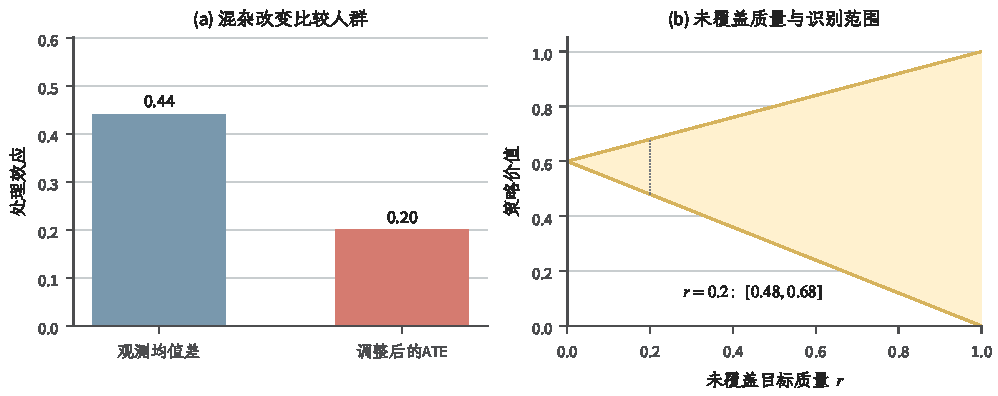
\includegraphics[width=\linewidth]{figures/01-mathematical-preliminaries/04-random-variables-distributions-and-causality/matplotlib/probability-discrete/causal-confounding-coverage.pdf}
  \caption{两个独立的教学构造。左图比较风险分层例子的观测均值差\(0.44\)与调整
  效应\(0.20\)。右图按式~\eqref{eq:causal-policy-value-bounds}绘制
  \([0.6(1-r),0.6(1-r)+r]\)。阴影为总体识别范围，不是抽样置信带；
  两个面板不表示同一数据集。}
  \label{fig:causal-confounding-coverage}
\end{figure*}

这里的策略只作一次行动。第~\ref{sec:decision-dynamic-programming}节建立序贯
策略后，必须逐时检查历史覆盖、时间变化的混杂及轨迹结果定义，不能把单步权重
直接套到整条轨迹。

\subsubsection{未观测混杂下的敏感性范围}
\label{sec:causal-sensitivity-ranges}

另一种缺口不是某类记录完全没有，而是相同已观测背景下仍存在未观测选择差异。
敏感性分析不强行断言该差异为零，而是规定其允许强度，检查结论随强度怎样变化。

先用一个最小线性模型定位偏差。设变量中心化，
\[
  T=\alpha U+\varepsilon_T,\qquad
  Y=\beta T+\gamma U+\varepsilon_Y,
\]
其中\(U,\varepsilon_T,\varepsilon_Y\)两两独立、方差有限，且
\(\operatorname{Var}(T)>0\)。理想设定\(T=t\)时，固定背景的结果对\(t\)的
导数为\(\beta\)。但只将\(Y\)对自然处理\(T\)作总体线性回归，得到
\begin{equation}
  \begin{aligned}
    \beta_{\mathrm{obs}}
    &=\frac{\operatorname{Cov}(T,Y)}{\operatorname{Var}(T)}\\
    &=\beta+
      \gamma\frac{\alpha\operatorname{Var}(U)}{\operatorname{Var}(T)}.
  \end{aligned}
  \label{eq:causal-linear-confounding-bias}
\end{equation}
这里用到了
\(\operatorname{Cov}(T,Y)=\beta\operatorname{Var}(T)
+\gamma\operatorname{Cov}(T,U)\)，以及
\(\operatorname{Cov}(T,U)=\alpha\operatorname{Var}(U)\)。
共同背景同时进入处理与结果，产生了第二项。若仅支持该偏差绝对值不超过
\(\Lambda\)，则
\(\beta\in[\beta_{\mathrm{obs}}-\Lambda,\beta_{\mathrm{obs}}+\Lambda]\)。
观测可以估计\(\beta_{\mathrm{obs}}\)，却不能在没有额外信息时把
\(\alpha,\gamma,\beta\)各自分开；改变函数形式也会改变敏感性参数的含义。

异质或非线性响应不一定有一个统一斜率修正量。仍记
\(\mu_t(x)=\mathbb E[Y\mid T=t,X=x]\)和\(e(x)=\mathbb P(T=1\mid X=x)\)。
在\(0<e(x)<1\)且相关条件期望有限时，定义选择偏差函数
\[
  \begin{aligned}
    b_1(x)&=\mathbb E[Y(1)\mid T=1,X=x]
            -\mathbb E[Y(1)\mid T=0,X=x],\\
    b_0(x)&=\mathbb E[Y(0)\mid T=1,X=x]
            -\mathbb E[Y(0)\mid T=0,X=x].
  \end{aligned}
\]
条件交换性蕴含\(b_1=b_0=0\)，但反过来只得到条件均值交换性，
不能推出完整潜在结果分布相同。比如两组都均值为零，一组恒等于零，另一组等概率
取\(1,-1\)，均值相同仍保留分布差异。

一致性给出
\(\mathbb E[Y(1)\mid T=1,X=x]=\mu_1(x)\)，再由全期望
\[
  \begin{aligned}
    \mathbb E[Y(1)\mid X=x]
    &=e(x)\mu_1(x)+(1-e(x))(\mu_1(x)-b_1(x))\\
    &=\mu_1(x)-(1-e(x))b_1(x).
  \end{aligned}
\]
另一侧有
\[
  \begin{aligned}
    \mathbb E[Y(0)\mid X=x]
    &=(1-e(x))\mu_0(x)+e(x)(\mu_0(x)+b_0(x))\\
    &=\mu_0(x)+e(x)b_0(x).
  \end{aligned}
\]
相减得到
\begin{equation}
  \tau(x)=\mu_1(x)-\mu_0(x)
  -(1-e(x))b_1(x)-e(x)b_0(x).
  \label{eq:causal-selection-bias-function}
\end{equation}
若领域知识仅支持
\(|b_1(x)|\leq\Gamma_1(x)\)及\(|b_0(x)|\leq\Gamma_0(x)\)，三角不等式给出
\begin{equation}
  \begin{aligned}
    \mu_1(x)-\mu_0(x)-\Delta(x)
    &\leq\tau(x)\\
    &\leq\mu_1(x)-\mu_0(x)+\Delta(x),
  \end{aligned}
  \label{eq:causal-sensitivity-bounds}
\end{equation}
其中\(\Delta(x)=(1-e(x))\Gamma_1(x)+e(x)\Gamma_0(x)\)。
重叠在目标总体几乎处处成立、潜在结果及相应控制量可积时，再对\(X\)平均便得到
ATE范围。该范围是当前偏差约束的有效包络；若还有限定结果范围或其他联合约束，
不能未经可达性检查就宣称它为锐界。

\(\Gamma_t\)是关于未观测差异的假设，不是样本自动生成的误差条。报告应展示在多大
强度下结论变号或越过决策阈值，而不只给一个恰好保留原结论的值。
其他有根据的假设也能缩小相容类。例如个体\term{单调性}（monotonicity）
\[
  Y(1)\geq Y(0)\quad\text{几乎必然}
\]
排除所有受损个体，故ATE至少为零，可以将有效下界提高到零。
它比“平均有益”更强。若已知个体效应位于\([-\rho,\rho]\)，支持缺口中的
\([-1,1]\)可换成更窄范围；平滑外推也必须作为新增机制限制声明。

跨环境资料可以提供另一种约束。若源环境有随机试验，目标环境给出协变量分布，
并假设条件效应在两环境相同，且目标协变量分布对源环境分布绝对连续，即源环境
的零概率背景集在目标环境中也为零概率，则
\[
  \tau_{\mathrm{target}}
  =\int\tau_{\mathrm{source}}(x)\,P_{X,\mathrm{target}}(\mathrm dx).
\]
这是条件效应稳定和目标覆盖共同给出的运输关系；在离散情形，覆盖要求目标中
出现的背景在源环境也有正概率。连续情形仅有拓扑支持包含还不够，应使用上述
绝对连续条件。它们都不是看到稳定预测关联就自动成立。
共同隐藏原因、选择过程或多个机制同步变化都可能产生稳定关联。

相容类也可用于第~\ref{sec:causal-counterfactual-recourse}节的反事实、补救与公平
目标。跨世界配对不同的模型可能同样解释试验边缘，却改变行动成功概率或公平判断。
此时应传播这些模型差异，而不是仅报告选定生成模型内的模拟精度。

\subsection{有限样本下的响应估计}
\label{sec:causal-response-estimation}

即使识别式成立，条件响应、处理概率与总体权重通常仍需从样本估计。比如调整法用
\(\widehat\mu_t\)代替\(\mu_t\)，再在目标背景样本上平均：
\[
  \widehat\tau
  =\frac1n\sum_{i=1}^n
    \bigl(\widehat\mu_1(X_i)-\widehat\mu_0(X_i)\bigr).
\]
这只是识别式的一种代入估计，不自动具有无偏性或某种收敛速度。拟合误差、目标样本
的抽样误差以及重复使用同一数据引入的依赖，仍须按第~\ref{sec:rv-inference}节
的估计与数据复用规则分析。采用样本拆分或交叉拟合时，应明确哪些样本拟合、哪些
样本评价，以及相应误差条件。

逆概率法还要估计倾向概率。很小但非零的真实概率允许总体识别，却可能使估计方差
很大；截断权重可改变偏差与方差，但不能被解释为凭空补足支持。更灵活的拟合器
或交叉拟合同样不能修复交换性错误。

部分识别时，估计对象可以是识别集合的端点或其外包络。识别集合在总体分布已知时
仍可能不是单点，表达机制歧义；\term{置信区间}来自有限样本，表达总体目标、
识别集合或端点的估计误差。对端点构造置信范围，还需按所用统计方法处理两个端点
共同的覆盖要求，不能把端点估计直接当作已知真界。

实际报告应分别列出相容机制留下的范围、抽样造成的不确定性，以及积分或优化中的
数值误差。增加样本主要改善第二项，改善算法主要影响第三项；改变设计、扩大目标
行动覆盖或加入可辩护的机制限制，才可能缩小第一项。尤其在效应符号或行动阈值附近，
应同时报告对支持处理、敏感性参数及目标总体选择的依赖。

\section{因果生成结构的表示}
\label{sec:causal-generating-structure}

前面把响应映射作为已知模型的接口，或把它放进与资料相容的候选类。现在打开这个
接口：培训先改变技能，技能再影响成绩，整体响应怎样由这些局部关系合成？需要记录
的不只有箭头，还包括每个变量的生成函数及未展开背景的联合分布。局部方程负责
产生数值，图负责记录输入关系；二者共同说明可以替换什么、替换后应重算什么。

\subsection{局部机制的结构方程表示}
\label{sec:causal-local-structural-equations}

把模型内需要解释的变量称为内生变量，把当前模型不再解释的背景称为外生变量。
“外生”是相对于模型边界而言，并不意味着这些量在现实中没有原因，也不自动意味着
它们彼此独立。进入某个变量生成函数的其他内生变量称为它的父变量，表示该局部机制
直接读取哪些输入。

\begin{definition}[无环结构因果模型]
  \label{def:causal-structural-model}
  本章的\term{结构因果模型}（structural causal model, SCM）由内生变量
  \(\bm V=(V_1,\ldots,V_d)\)的可测状态空间、外生背景
  \(\bm U=(U_1,\ldots,U_d)\)的联合分布及可测结构函数组成：
  \begin{equation}
    V_j=f_j(\operatorname{pa}_j,U_j),
    \qquad j=1,\ldots,d.
    \label{eq:causal-scm-definition}
  \end{equation}
  其中\(\operatorname{pa}_j\)收集进入第\(j\)个函数的其他内生变量。
  \term{无环}（acyclic）要求存在节点次序\(j_1,\ldots,j_d\)，使每个函数的
  内生输入都来自次序中更早的节点。外生分量可以相关。
\end{definition}

把每个内生变量画成节点，在\(V_k\)作为输入进入\(f_j\)时画箭头\(V_k\to V_j\)，
便得到有向无环图，简称DAG。上述求值次序已足以理解无环性，不需要先学习图排序
算法。SCM的箭头具有生成语义；若箭头只用于表示联合分布的条件分解，就不能据此
判断改变输入的后果\scite{math-pearl2009causality}

例如，培训\(T\)、技能\(M\)和成绩\(Y\)可以写成
\[
  T=f_T(U_T),\qquad
  M=\alpha T+U_M,\qquad
  Y=\beta T+\gamma M+U_Y.
\]
这里的直接输入关系为\(T\to M\)、\(T\to Y\)、\(M\to Y\)。若
\(U_T,U_M,U_Y\)相关，处理选择还可能与技能或成绩背景相联系；仅画出这三条内生边
不足以表示全部共同背景。要使用独立噪声DAG的概率规则，必须另行要求这些背景独立，
或把相关性的共同来源显式放进模型。

有限维模型可以把局部函数写成\(f_{j,\bm\theta_j}\)，并用
\(\bm\theta=(\bm\theta_1,\ldots,\bm\theta_d)\)汇集参数。上例的
\(\alpha,\beta,\gamma\)是局部作用参数；一般SCM则不必属于有限维函数族。
指定关系但不知道函数，或拟合函数却没有确定它的因果语义，都仍留下结构上的未知。

\subsection{局部机制的复合与响应生成}
\label{sec:causal-mechanism-composition}

有了局部方程，定义~\ref{def:causal-response-interface}假定的自然映射就可以
实际构造。无环次序让每一步只读取已经得到的值，因此既给出计算过程，也排除了
同一背景下出现多个自然解的歧义。

\begin{theorem}[无环机制的唯一可测响应]
  \label{thm:causal-acyclic-response}
  对定义~\ref{def:causal-structural-model}中的模型，每个背景
  \(\bm u\)唯一确定一组满足所有结构方程的内生取值。
  所得自然映射\(F_M:\mathcal U\to\mathcal V\)可测。将任意指定的一组方程
  替换为常量方程后，所得映射\(F_M^a\)同样存在、唯一且可测。
  对单变量理想干预，响应\((t,\bm u)\mapsto R_M(t,\bm u)\)联合可测。
\end{theorem}
\begin{proof}
  取符合无环性的次序\(j_1,\ldots,j_d\)。第一个变量没有内生父变量，
  因而\(v_{j_1}=f_{j_1}(u_{j_1})\)唯一确定，且是\(\bm u\)的可测函数。
  假设前\(k-1\)个变量已唯一确定为可测函数。第\(k\)个方程的父变量都在其中，
  将这些函数及\(u_{j_k}\)代入可测的\(f_{j_k}\)，便得到唯一且可测的
  \(v_{j_k}\)。归纳到\(d\)，得到满足全部方程的可测向量\(F_M(\bm u)\)。
  任何另一组解在第一个坐标都必须相同；逐坐标应用同一理由，便证明唯一性。

  常量替换只删除输入，不增加逆向依赖，原次序仍可使用。被替换坐标直接取行动
  指定值，其余坐标按同样归纳求出，从而得到\(F_M^a\)。
  若把处理值\(t\)也作为输入，被替换坐标是乘积空间上的投影
  \((t,\bm u)\mapsto t\)，其余步骤仍是可测函数的复合，因此
  \(F_M^{a(t)}(\bm u)\)及其结果坐标\(R_M(t,\bm u)\)联合可测。
\end{proof}

自然分布是\((F_M)_{\#}P_{\bm U}\)，干预分布是
\((F_M^a)_{\#}P_{\bm U}\)。两个推前共用同一个背景分布，只改变生成映射。
若理想干预值恰好等于该背景下的自然处理值，那么自然解也满足替换后的全部方程；
由唯一性，两组解相同。这也证明了这种构造中的一致性，而不只是另行假定
\(Y=Y(T)\)。

若结果方程为\(Y=f_Y(T,X,U_Y)\)，且\(X\)不受处理干预影响，则
\begin{equation}
  Y(t)=f_Y(t,X,U_Y).
  \label{eq:causal-scm-potential-outcome}
\end{equation}
因此\(\mathcal L(Y(t))=\mathcal L(Y\mid\operatorname{do}(T=t))\)。
若结果还依赖处理会改变的技能\(M\)，则必须先重算\(M(t)\)，不能仍代入事实技能。
对上面的线性机制，
\[
  M(t)=\alpha t+U_M,\qquad
  Y(t)=(\beta+\gamma\alpha)t+\gamma U_M+U_Y,
\]
所以整体响应导数为\(\beta+\gamma\alpha\)，不只是局部结果方程中固定\(M\)
时的偏导数\(\beta\)。取\(\alpha=2,\beta=1,\gamma=3\)，增加一单位培训使成绩
增加\(7\)，其中直接贡献为\(1\)，经技能传递的贡献为\(6\)。
对可微的非线性机制\(M=f_M(T,U_M)\)、\(Y=f_Y(T,M,U_Y)\)，链式法则给出
\[
  \frac{\partial R_M(t,\bm u)}{\partial t}
  =
  \frac{\partial f_Y}{\partial t}
  +
  \frac{\partial f_Y}{\partial m}
  \frac{\partial f_M}{\partial t},
\]
各偏导数均在该背景的干预取值处计算。这连接了第~\ref{sec:causal-local-response}节
的整体局部变化与本节的局部方程；对它再作总体平均，仍须检查导数与积分交换条件。

在外生噪声相互独立时，还可以用局部概率核表达同一计算。记
\[
  K_j(B\mid\bm v_{\operatorname{pa}_j})
  =
  \mathbb P\bigl(f_j(\bm v_{\operatorname{pa}_j},U_j)\in B\bigr).
\]
每个核都由机制及噪声分布指定，沿无环次序复合这些核便得到联合分布。独立性保证
当前噪声不会被已经生成的变量额外筛选。若这些核具有质量函数或密度，则
\[
  p(\bm v)=\prod_{j=1}^d p(v_j\mid\operatorname{pa}_j).
\]
理想干预把处理核换成点质量，其余核保持原样，于是得到\term{截断分解}
\begin{equation}
  p(\bm v_{-T}\mid\operatorname{do}(T=t))
  =
  \prod_{j:V_j\ne T}
  p(v_j\mid\operatorname{pa}_j)\big|_{T=t}.
  \label{eq:causal-truncated-factorization}
\end{equation}
这里\(\bm v_{-T}\)表示删除处理坐标后的变量集合。公式来自机制替换，不是对
任意概率分解删除一个因子都能得到因果分布。外生噪声相关时，上述独立核复合一般
不成立；应回到完整背景的推前，或显式展开相关来源。

局部因子必须使用结构机制指定的版本。观测分布只在父变量实际出现的支持上确定
条件分布；干预若产生了未见过的父变量组合，机制可以给出答案，但资料未必能识别
该答案。随意补一个支持外的条件密度，不会把模型外推变成数据结论。

对简单结构\(X\to T\)、\(X\to Y\)、\(T\to Y\)，用独立的新随机量按
\(q(t\mid x)\)分配处理，并保持其余独立噪声机制不变，得到
\begin{equation}
  p^q(x,t,y)=p(x)q(t\mid x)p(y\mid t,x).
  \label{eq:causal-stochastic-intervention}
\end{equation}
这正是第~\ref{sec:causal-intervention-potential-outcomes}节随机干预构造的局部
表达。确定性策略用点质量核表示，不必假装它有通常的Lebesgue密度。
策略若同时改变参与人群、结果测量或其他机制，就不能只替换处理因子。
更一般的机制替换也需要保证修改后的方程有明确解；添加依赖关系时，原无环次序
可能不再适用。

循环方程说明这一边界并非形式问题。例如\(V_1=V_2+1,V_2=V_1\)无解，而
\(V_1=V_2,V_2=V_1\)有无穷多组解。反馈系统可能需要动态演化、平衡选择或额外
唯一性条件，不能直接套用本节递归证明。

\subsection{变量关系的图表示与调整条件}
\label{sec:causal-graph-adjustment}

完整求解SCM可以得到响应，但有时只需回答一个较窄的问题：哪些变量适合用来调整
处理组之间的背景差异？图保留直接输入关系而暂时略去具体函数，因而能在一类机制
上共同作出判断。下面先看三种局部关系，再检查全图路径，最后把判断接到已经证明
的调整公式。

\subsubsection{局部因果关系与调整影响}
\label{sec:causal-local-path-patterns}

结构\(T\leftarrow X\to Y\)把\(X\)称为\(T\)与\(Y\)的
\term{共同原因}（common cause）。即使处理并不影响结果，不同\(X\)人群接受
处理的比例不同，也会使\(T,Y\)在自然记录中相关。这是混杂产生的一种方式。
第~\ref{sec:causal-adjustment-identification}节的风险分层算例正是通过在同一背景层
比较，再用同一目标权重平均，消除了由两组构成不同造成的差异。

结构\(T\to M\to Y\)中的\(M\)是\term{中介变量}（mediator）：处理对结果的
一部分影响经过它传递。若目标是总效应，固定\(M\)会阻断这部分变化；若研究同时
设定\(T=t,M=m\)的响应，则需明确这是不同的联合干预。
在线性例子中，固定中介后的处理系数为\(\beta\)，让中介随处理变化的总系数为
\(\beta+\gamma\alpha\)。这并不建立一般路径效应的识别公式，只说明两种目标不同。

结构\(T\to C\leftarrow Y\)中的\(C\)是\term{碰撞点}（collider），两条箭头
在此相遇。不以\(C\)筛选时，这条路径本身不要求两端相关；一旦给定\(C\)，却可能
引入关联。例如两个独立能力共同决定总分，入选要求总分超过阈值且两项能力可以
补偿，那么入选者中一项能力较弱的人往往需要另一项更强。若入选规则改成两项能力
分别超过各自阈值，这种负关联未必出现。关系的方向取决于选择机制，不能把选择
后的相关解释为一种能力造成另一种能力。

图~\ref{fig:causal-local-path-patterns}中的双边框表示中间变量被加入条件集。
共同原因和中介在该路径上都是非碰撞点，给定后会关闭路径；碰撞点的行为相反。
这解释了为何“控制更多变量”不是普遍有效的做法，也预告了局部路径能否关闭与
全图是否仍有其他路径是两件事。
\begin{figure*}[htbp]
  \centering
  \begin{tikzpicture}[figure picture,x=1mm,y=1mm,
  causalnode/.style={circle,draw=FigureStroke,fill=none,line width=1pt,
    minimum size=7mm,inner sep=0pt,font=\figurefont\mdseries\footnotesize},
  conditionednode/.style={causalnode,draw=FigureYellow,
    double=white,double distance=0.7pt},
  causaledge/.style={-{Stealth[length=2.2mm,width=1.4mm]},
    draw=FigureStroke,line width=1.1pt},
  paneltitle/.style={font=\figurefont\mdseries\footnotesize,text=FigureInk},
  panellabel/.style={font=\figurefont\mdseries\small,text=FigureInk},
  note/.style={font=\figurefont\mdseries\footnotesize,
    text=FigureMuted,align=center,fill=none}]
  \path[use as bounding box] (0,-10) rectangle (169,38);
  \draw[FigureGrid,line width=0.6pt] (56,-8)--(56,36);
  \draw[FigureGrid,line width=0.6pt] (112,-8)--(112,36);

  \node[panellabel,anchor=west] at (1,33) {(a)};
  \node[paneltitle] at (28,33) {共同原因};
  \node[conditionednode] (fork-x) at (28,22) {\(X\)};
  \node[causalnode] (fork-t) at (13,11) {\(T\)};
  \node[causalnode] (fork-y) at (43,11) {\(Y\)};
  \draw[causaledge] (fork-x)--(fork-t);
  \draw[causaledge] (fork-x)--(fork-y);
  \node[note] at (28,-3) {给定\(X\)时关闭路径};

  \node[panellabel,anchor=west] at (57,33) {(b)};
  \node[paneltitle] at (84,33) {中介链};
  \node[causalnode] (chain-t) at (67,16) {\(T\)};
  \node[conditionednode] (chain-m) at (84,16) {\(M\)};
  \node[causalnode] (chain-y) at (101,16) {\(Y\)};
  \draw[causaledge] (chain-t)--(chain-m);
  \draw[causaledge] (chain-m)--(chain-y);
  \node[note] at (84,-3) {给定\(M\)时关闭路径};

  \node[panellabel,anchor=west] at (113,33) {(c)};
  \node[paneltitle] at (140,33) {碰撞点};
  \node[causalnode] (collider-t) at (125,22) {\(T\)};
  \node[causalnode] (collider-y) at (155,22) {\(Y\)};
  \node[conditionednode] (collider-c) at (140,11) {\(C\)};
  \draw[causaledge] (collider-t)--(collider-c);
  \draw[causaledge] (collider-y)--(collider-c);
  \node[note] at (140,-3) {不给定时关闭\\给定\(C\)时打开};
\end{tikzpicture}

  \caption{共同原因、中介与碰撞点的局部路径。双边框表示节点已加入条件集。
  共同原因和中介是非碰撞点，给定后关闭这条路径；给定碰撞点则打开原本关闭的
  路径。路径打开表示图不再保证相应独立性，并不指定相关的大小或正负。}
  \label{fig:causal-local-path-patterns}
\end{figure*}

\subsubsection{全图路径分离与概率约束}
\label{sec:causal-global-path-separation}

较大图中，关闭一个局部片段仍可能留下另一条联系。设
\(\mathcal G=(V,E)\)是有向无环图，\(V\)是节点集、\(E\)是有向边集。
下面沿用定义~\ref{def:graph-theory-d-separation}的图分离判据，
在生成模型中解释它怎样约束随机变量的条件独立。路径仍指底层图中相邻且互不重复
的节点序列，有向路径才要求沿箭头前进；祖先和后代均不包括节点自身。

\begin{definition}[图分离与概率独立的记号]
  \label{def:causal-d-separation}
  对两两不交的节点集\(A,B,S\)，其中\(A,B\)非空，
  \(A\perp_{\mathcal G}B\mid S\)表示图中连接\(A,B\)的每条路径都被\(S\)
  阻断；活跃路径的碰撞与非碰撞规则沿用定义~\ref{def:graph-theory-d-separation}。
  若各节点承载随机变量，\(X_A\perp X_B\mid X_S\)则表示给定\(X_S\)后，
  \(X_A,X_B\)的条件联合分布分解为条件边缘分布的乘积。
  前一个记号只依赖图，后一个记号依赖概率分布；二者之间的联系需要模型假设。
\end{definition}

碰撞点是相对于某一条路径而言的，同一节点在不同路径上可以扮演不同角色。
给定其后代也可能传回选择信息，因此不能只检查碰撞点本身是否在条件集。
以同时含有
\[
  X\to M\to Y,\qquad X\to C\leftarrow Y,\qquad C\to D
\]
的图为例，\(X,Y\)之间有经过\(M\)和经过\(C\)的两条路径。四种条件集给出
不同判断：
\begin{itemize}
  \item \(S=\varnothing\)：经过\(M\)的链活跃，经过\(C\)的碰撞路径关闭，
  因而两端仍然d-连接。
  \item \(S=\{M\}\)：链被关闭，碰撞路径也仍关闭，所以
  \(X\perp_{\mathcal G}Y\mid M\)。
  \item \(S=\{M,C\}\)：链仍关闭，但给定碰撞点打开下方路径，两端重新d-连接。
  \item \(S=\{M,D\}\)：给定碰撞点的后代也打开下方路径，两端同样d-连接。
\end{itemize}
图~\ref{fig:causal-d-separation-paths}显示第二种情形。这个例子在本章即可逐路
检查；一般路径、分离与图分解的计算工具已在第~\ref{chap:graph-theory}章建立。
\begin{figure}[htbp]
  \centering
  \begin{tikzpicture}[figure picture,x=1mm,y=1mm,
  causalnode/.style={circle,draw=FigureStroke,fill=none,line width=1pt,
    minimum size=7mm,inner sep=0pt,font=\figurefont\mdseries\footnotesize},
  conditionednode/.style={causalnode,draw=FigureYellow,
    double=white,double distance=0.7pt},
  causaledge/.style={-{Stealth[length=2.2mm,width=1.4mm]},
    draw=FigureStroke,line width=1.1pt},
  note/.style={font=\figurefont\mdseries\footnotesize,
    text=FigureMuted,align=center,fill=none}]
  \path[use as bounding box] (0,-22) rectangle (112,32);
  \node[note,text=FigureInk] at (56,27) {条件集\(S=\{M\}\)};
  \node[causalnode] (dsep-x) at (16,14) {\(X\)};
  \node[conditionednode] (dsep-m) at (56,14) {\(M\)};
  \node[causalnode] (dsep-y) at (96,14) {\(Y\)};
  \node[causalnode] (dsep-c) at (56,-1) {\(C\)};
  \node[causalnode] (dsep-d) at (56,-16) {\(D\)};
  \draw[causaledge] (dsep-x)--(dsep-m);
  \draw[causaledge] (dsep-m)--(dsep-y);
  \draw[causaledge] (dsep-x)--(dsep-c);
  \draw[causaledge] (dsep-y)--(dsep-c);
  \draw[causaledge] (dsep-c)--(dsep-d);
\end{tikzpicture}

  \caption{多条路径下的d-分离。双边框节点\(M\)属于条件集，上方链式路径关闭；
  碰撞点\(C\)及其后代\(D\)都未给定，下方路径也关闭。若再把\(C\)或\(D\)
  加入条件集，下方路径就会打开，说明增加条件可能破坏原有的分离。}
  \label{fig:causal-d-separation-paths}
\end{figure}
\FloatBarrier

\begin{definition}[因果Markov性]
  \label{def:causal-markov-property}
  分布\(P\)相对于因果DAG \(\mathcal G\)满足\term{因果Markov性}
  （causal Markov property），是指对任意两两不交的节点集\(A,B,S\)，
  \[
    A\perp_{\mathcal G}B\mid S
    \quad\Longrightarrow\quad
    \bm V_A\perp\bm V_B\mid\bm V_S.
  \]
  其中\(\bm V_A,\bm V_B,\bm V_S\)分别收集对应节点的随机变量。
\end{definition}

左边是图规则，右边是分布性质。因果Markov性把前者的阻断结论转成条件独立；
它没有说d-连接一定产生统计依赖，也没有从观测独立直接反推箭头。它与时序过程
“给定当前状态后无须更早历史”的Markov性质使用不同对象和条件集，不能只因名称
相同就互相代入。

对DAG，这一全局表述等价于局部表述：每个变量在给定父变量后，与其非后代中除
自身和父变量外的变量条件独立。独立外生噪声的无环SCM满足这一性质。
直观上，非后代及父变量不读取当前节点的独立噪声；给定父变量后，当前变量剩下
的随机性就来自这一噪声。对局部核乘积，按逆向求值次序逐个积分掉无关后代，
每次被消去的条件核积分为一，由此保留所需的局部条件因子。分解与d-分离的
全局对应是DAG的标准结论\scite{math-pearl2009causality}
图分解与消元工具见第~\ref{chap:graph-theory}章；把图分离转成概率独立，
还需要这里的DAG分解或生成机制条件，不能只凭连接结构推出。
若背景相关而共同来源没有入图，不能仍对这个省略后的DAG直接宣称因果Markov性。

\subsubsection{后门条件下的调整变量选择}
\label{sec:causal-backdoor-selection}

第~\ref{sec:causal-adjustment-identification}节直接假定条件交换性，再证明调整
识别。现在可以反过来问：一张已经具有生成语义的图，能否为调整变量的选择提供
充分依据？从\(T\)到\(Y\)且第一条边指向\(T\)的路径称为
\term{后门路径}（back-door path），它从处理的自然生成来源进入比较，而非沿
处理对结果的有向作用出发。

\begin{definition}[单处理、单结果的后门准则]
  \label{def:causal-backdoor-criterion}
  设\(T,Y\)是因果DAG中的不同节点，\(Z\)与\(\{T,Y\}\)不交。若\(Z\)
  不含\(T\)的后代，且给定\(Z\)阻断所有从\(T\)到\(Y\)、第一条边指向
  \(T\)的路径，则称\(Z\)满足相对于\((T,Y)\)的
  \term{后门准则}（back-door criterion）。
\end{definition}

阻断按定义~\ref{def:causal-d-separation}判断，把碰撞点放进\(Z\)可能打开
原本关闭的路径。最基本的代表图为\(Z\to T,Z\to Y,T\to Y\)，独立噪声机制给出
\[
  p(z,t,y)=p(z)p(t\mid z)p(y\mid t,z).
\]
将处理机制替换为常量\(t\)后，
\(p(z,y\mid\operatorname{do}(T=t))=p(z)p(y\mid t,z)\)。再对背景积分，得到
\begin{equation}
  p(y\mid\operatorname{do}(T=t))
  =
  \int p(y\mid t,z)p(z)\,\mathrm dz.
  \label{eq:causal-backdoor-adjustment}
\end{equation}
离散背景用求和，一般空间用对\(P_Z\)的核积分。对结果再取期望，就回到
式~\eqref{eq:causal-g-formula}的调整表示。

一般后门准则在独立噪声无环SCM、图正确包含相关共同原因且干预保留其他机制的
条件下，给出同样的调整结论\scite{math-pearl2009causality}
阻断全部后门路径排除了自然处理选择沿这些路径携带的背景差异，非后代条件保证
用于平均的\(Z\)不先被行动改变。这些是生成结构对交换性的充分支持，而不是只由
一个观测分布满足Markov性就能推出的干预结论。即使图条件成立，要从观测资料
确定积分中的局部响应，还需要目标总体内所用处理的支持条件；图不会填补空白
协变量--处理组合。

三个局部图可以核对变量角色。在\(T\leftarrow X\to Y\)中，\(X\)关闭后门；
在\(T\to M\to Y\)中，\(M\)是后代，固定它会改变总效应目标；
在\(T\to C\leftarrow Y\)中，空条件集已经关闭碰撞路径，加入\(C\)反而打开它。
因此，处理前测量、与结果相关或能提高预测精度，都不是充分的调整标准。
后门准则是充分条件，不是识别的必要条件；它不适用时，随机设计、其他识别规则
或更具体的机制假设仍可能确定所选目标。

\section{因果生成结构的推断}
\label{sec:causal-structure-discovery}

此前给定图和局部机制，便能生成响应或支持调整。实际研究还可能不知道哪些变量
直接相连，也不知道相连以后怎样传递变化。前一项是变量关系的推断，后一项是局部
机制的推断；它们共同决定响应，但所需信息并不相同。一个模型能拟合观测数据，
不代表它的箭头、结构函数和同背景反事实都已经被唯一确定。

\subsection{变量关系的推断}
\label{sec:causal-relation-inference}

从图推出分布约束与从分布反推图，是方向相反的两项任务。要用条件独立排除候选
关系，需要说明哪些独立是真正的结构阻断，哪些可能来自参数抵消。资料制度也很
重要：同分布观察、受控干预和不同环境提供的限制不一样。

\subsubsection{观测资料下的关系识别}
\label{sec:causal-observational-structure}

\begin{definition}[相对于DAG的忠实性]
  \label{def:causal-faithfulness}
  分布\(P\)相对于DAG \(\mathcal G\)满足\term{忠实性}（faithfulness），若对
  任意两两不交的节点集\(A,B,S\)，
  \[
    \bm V_A\perp\bm V_B\mid\bm V_S
    \quad\Longrightarrow\quad
    A\perp_{\mathcal G}B\mid S.
  \]
\end{definition}
忠实性要求分布中出现的条件独立能由图结构解释，不是由特殊参数抵消、确定性
约束或未处理的误差相关造成。因果Markov性给出正向蕴含，忠实性补上反向蕴含，
两者不能互相替代。

例如，设\(X,U_M,U_Y\)相互独立，
\(M=\alpha X+U_M\)，\(Y=\beta X+\gamma M+U_Y\)。
当\(\alpha,\gamma\ne0\)且\(\beta=-\gamma\alpha\)时，
\(Y=\gamma U_M+U_Y\)与\(X\)独立，但图中直接路径\(X\to Y\)及
\(X\to M\to Y\)都存在。两条贡献恰好抵消，说明无环与独立噪声并不自动保证
忠实性。接近这种抵消时，非零依赖还可能非常弱，有限样本中难以检出。

只考察三个节点且没有其他路径时，链
\(X\to Z\to Y\)、反向链\(X\leftarrow Z\leftarrow Y\)和共同原因
\(X\leftarrow Z\to Y\)都蕴含
\[
  X\perp Y\mid Z,
\]
却一般不蕴含\(X\perp Y\)。条件独立模式无法区分中间变量在传递作用还是造成
共同变化。碰撞结构\(X\to Z\leftarrow Y\)则蕴含\(X\perp Y\)，给定中间
节点后可能相关；加上忠实性，才能把这种模式差别用作反向辨识的依据。
这回用了图~\ref{fig:causal-local-path-patterns}，但大图还必须检查所有其他路径。

\begin{definition}[Markov等价与等价类]
  \label{def:causal-markov-equivalence}
  同一节点集上的两张DAG若具有完全相同的d-分离关系，就称它们
  \term{Markov等价}（Markov equivalent）。
  与给定图Markov等价的全部DAG组成其
  \term{Markov等价类}（Markov equivalence class, MEC）。
\end{definition}

图的\term{骨架}（skeleton）是忽略箭头方向后的邻接关系。
\term{无屏蔽碰撞结构}（unshielded collider）指
\(X\to Z\leftarrow Y\)，并且两端\(X,Y\)不相邻。没有两端的直接边，才使
这个局部碰撞的差异能够通过两端的分离关系表现出来。
标准判据是：两张DAG Markov等价，当且仅当具有相同骨架和相同无屏蔽碰撞结构
\scite{pgm-structure-learning-chickering2002}

判据的必要性可以直接从全部路径证明。先说明DAG中任意两个非相邻节点都有一个
不含端点的d-分离集。选其中一个节点\(v\)，使另一个节点\(w\)不是它的后代；
无环性保证至少有这样一个选择。令条件集为\(v\)的父节点集。
任意从\(v\)到\(w\)的路径若第一条边指向\(v\)，就经过一个父节点；因两端
不相邻，该父节点是内部非碰撞点，路径被阻断。
若第一条边从\(v\)向外，路径不可能一直沿箭头到达非后代\(w\)。沿路径第一次
改变箭头方向时，出现一个碰撞点\(c\)，此前的有向前缀说明\(c\)是\(v\)的
后代。\(c\)及其任何后代都不可能成为\(v\)的父节点，否则形成有向环；
故这个碰撞点没有被条件集打开，路径仍被阻断。两类覆盖了全部路径。
相邻节点之间的单边路径则没有内部点，不可能被任何不含端点的条件集阻断。
因此，骨架不同必导致d-分离关系不同。

再考虑同一骨架上的无屏蔽三点结构\(X-Z-Y\)。两端不相邻，按上段存在分离集。
若\(Z\)不是碰撞点，任何分离集都必须包含\(Z\)，否则长度为二的这条路径
仍然活跃；若\(Z\)是碰撞点，任何分离集都不能包含\(Z\)，否则该路径被打开。
因此，中点碰撞状态不同也必然改变d-分离关系。其他路径可能增加分离要求，却
不会消除这条长度为二的路径对每个分离集施加的限制。

充分性需要控制所有较长路径，这里引用完整结构判据，不把上述必要性论证冒充
双向证明\scite{pgm-structure-learning-chickering2002}
理解等价类内部的方向变化还可借助\term{覆盖边}（covered edge）：边
\(X\to Y\)若满足
\[
  \operatorname{pa}(Y)=\operatorname{pa}(X)\cup\{X\},
\]
便是覆盖边，这里\(\operatorname{pa}(X)\)表示父节点集合。
覆盖边反转定理说明，反转这种边后仍为DAG，并保持全部d-分离关系
\scite{pgm-structure-learning-chickering2002}
从局部因子看，对给定共同父变量，这一步把
\[
  p(x\mid\operatorname{pa}(X))
  p(y\mid x,\operatorname{pa}(X))
  =
  p(y\mid\operatorname{pa}(X))
  p(x\mid y,\operatorname{pa}(X))
\]
重新分解，不改变两变量的条件联合分布。因子应取相容的条件版本；这个等式解释
分布重参数化，却没有单独证明全图等价，更没有证明两张指定图之间存在变换序列。
完整变换定理进一步保证，任意两张已知Markov等价的DAG，可以经有限次覆盖边
反转相互到达，每个中间图都保持无环且等价。这是等价类内的可达性结论，不能
代替结构判据的充分性证明\scite{pgm-structure-learning-chickering2002}

等价类可以用部分有向图表示：全部等价图都同意的方向保留箭头，其余边保持无向。
在因果Markov性、忠实性、无环和无潜在混杂等条件下，纯观测条件独立信息一般
只能识别这样的等价类。输出一条无向边并非一定表示算法未完成；它可能记录总体
观测分布本身无法决定的方向。增加同分布样本能改善独立性判断，却不会制造类内
所缺少的方向信息。

这里还隐含了变量覆盖。所有相关共同原因都已纳入可观测变量时，称满足因果充分性。
潜在共同原因能让两个可观测节点相关，却不应被硬解释成其中一个直接导致另一个。
允许潜在混杂或选择后，输出往往需要扩大到带不同端点标记的部分图，分别表示
已确定的祖先关系、可能方向和无法排除的隐藏共同原因。测量误差以及按碰撞点
选择样本也会改变独立模式，不应一律视为新增因果边。

有限样本中的关系发现还要通过检验或评分近似总体判断。以
\(H_0:V_i\perp V_j\mid\bm V_S\)为原假设，若约束型算法在未拒绝独立时
删除候选边，那么第一类错误把真实独立误判为依赖，可能保留虚假边；
第二类错误把实际依赖误判为独立，可能删除真实边。后续搜索与定向会传播错误，
评分型算法则不能直接套用这组对应。高维条件集减少每层有效样本，近忠实边界上
的弱依赖尤其难判断。结构学习的一致性必须同时说明总体的Markov与忠实条件、
检验或评分的渐近性质、候选图范围，以及搜索能否达到目标；一张确定输出图
不代表因果方向已经唯一。

\subsubsection{干预与环境变化下的方向识别}
\label{sec:causal-interventional-structure}

要打破观测方向歧义，需要增加具有不同约束的信息。理想干预切断目标变量的原
进入机制：若随机设置\(X\)后，\(Y\)的分布随设置值改变，在其余机制不变、
行动确实只作用于\(X\)的模型中，这支持\(X\)位于\(Y\)的上游。反之，没有
观察到分布改变并不自动排除作用，机制抵消、剂量范围或检验能力都可能影响判断。
对多个节点施加适当干预可缩小观测等价类，但能缩小到什么程度取决于干预覆盖。

这一证据必须按实际执行解释。干预目标未知、执行不完全，或干预同时改变测量、
选择和其他机制时，都应将这些不确定性纳入模型。不能把“鼓励参加培训”无条件
等同于“把培训处理设为指定值”，也不能把伴随整套制度改变的干预解释成单个
节点的理想替换。

不同环境也可能提供方向限制。设环境标签为\(E\)，若假定环境只改变输入\(X\)
的分布，而机制\(Y=f_Y(X,U_Y)\)及独立噪声\(U_Y\)的分布保持不变，那么
各环境在共同支持上的\(P(Y\mid X,E=e)\)应相同；反向条件分布
\(P(X\mid Y,E=e)\)却可能随输入分布变化。这里稳定性来自已声明的生成假设，
并非看到一个稳定条件分布就证明了箭头。

潜在共同原因可以在所有已观察环境中稳定，环境变化也可能太弱，未能打破错误
方向；选择规则同步变化还可能制造稳定关联。应分别说明哪些背景分布或局部
机制允许改变，哪些保持不变，环境是否直接影响结果，以及稳定性究竟是模型
假设、检验对象还是经验线索。机制知识和对隐藏混杂、弱依赖、选择过程的
敏感性分析，共同限制候选关系，不能由增加同分布样本替代。

对于反馈环、随时间改变的机制或处理定义不稳定的系统，无环静态模型本身可能
不合适，需要改用动态或循环模型并重新定义行动；方向识别不能先忽略模型边界，
再用搜索算法的精度弥补。

\subsection{局部机制的推断}
\label{sec:causal-local-mechanism-inference}

即使关系已经给定，箭头也没有给出作用大小、非线性形状和背景分布。
局部机制推断要在声明的函数族、噪声条件和观测制度内估计这些未知部分。
它可以回用第~\ref{sec:rv-inference}节的有限维参数或函数估计，但必须先明确
估计对象是否具有所需的干预含义。

例如，对已给定的父变量向量\(\bm P_j\)，假设局部方程为
\[
  V_j=\theta_{j0}+\bm\theta_j^{\mathsf T}\bm P_j+\varepsilon_j,
  \qquad
  \mathbb E[\varepsilon_j\mid\bm P_j]=0.
\]
令\(\bm Z_j=(1,\bm P_j^{\mathsf T})^{\mathsf T}\)，并令
\(\bm\vartheta_j=(\theta_{j0},\bm\theta_j^{\mathsf T})^{\mathsf T}\)。
若二阶矩有限且
\(\bm Q_j=\mathbb E[\bm Z_j\bm Z_j^{\mathsf T}]\)可逆，乘以\(\bm Z_j\)再取
期望得到
\[
  \mathbb E[\bm Z_jV_j]=\bm Q_j\bm\vartheta_j,\qquad
  \bm\vartheta_j
  =\bm Q_j^{-1}\mathbb E[\bm Z_jV_j].
\]
因此在这些条件下，局部参数可由总体矩识别。独立同分布样本中的对应矩估计为
\[
  \widehat{\bm\vartheta}_j
  =
  \left(\frac1n\sum_{i=1}^n\bm Z_{ij}\bm Z_{ij}^{\mathsf T}\right)^{-1}
  \left(\frac1n\sum_{i=1}^n\bm Z_{ij}V_{ij}\right),
\]
前提是样本矩可逆。误差、区间和正则化处理仍属于统计估计问题。真实父变量
存在确定性共线时，矩方程不能唯一确定各系数；遗漏共同背景造成条件噪声均值
非零时，拟合得到的斜率也不再自动等于局部结构参数。

在培训例子里，可以分别拟合技能方程和成绩方程，再复合为
\(\widehat\beta+\widehat\gamma\widehat\alpha\)。结果方程中的
\(\widehat\beta\)只是固定技能时的局部系数，不应独自报告为总效应。这样从
局部估计传到整体响应时，还须传播多个估计量的共同误差。

非参数情形也要区分三个层次。观测资料可以在父变量支持上估计
\(P(V_j\mid\operatorname{pa}_j)\)；把这个条件核解释为干预下保持不变的机制，
还需要正确关系、噪声及机制不变假设；再要求同一背景下不同输入怎样配对，则
需要更强的结构表示。同一组局部条件核可以由不同结构函数和背景耦合实现。
第~\ref{sec:causal-factual-counterfactual}节的两种跨世界配对已经说明，边缘
分布相同不决定已知事实后的替代结果。因此，仅拟合条件分布不能自动唯一恢复
个体响应、反事实公平或行动成功概率。

结构函数和背景的重新参数化还可能给出完全相同的可观测与干预分布；一般SCM
不应被承诺为唯一可恢复。若采用加性独立噪声、特定函数形状或支持外平滑外推，
必须把这些限制写进候选机制类，而不能把拟合优度当成它们已被验证。
观测支持外的行动尤其依赖外推，残差诊断也不能单独证明全部背景独立和机制不变。

实际可保留候选对\((\mathcal G,\{f_j\},P_{\bm U})\)，逐一生成所关心的响应，
再把这些答案送回第~\ref{sec:causal-partial-identification-sensitivity}节的
识别集合。关系不确定、局部参数或函数不确定、跨世界背景配对不确定可能贡献
不同范围；样本有限还会增加估计误差。把这些来源分别传到平均效应、策略价值
或补救约束，才不会用一个最优拟合模型掩盖其他同样相容的行动后果。

\section{本章小结}
\label{sec:causal-inference-summary}

开篇的培训问题不能只由两组成绩差回答，因为自然接受处理的人可能具有不同背景。
给定生成模型和背景分布以后，响应映射能计算主动改变处理的后果；得知某人的事实
以后，则先更新背景分布，再在同一背景下改变行动。前者改变生成规则，事实条件化
改变对背景的认识，两步不能混成从干预总体重新抽一个人。

响应比较有不同口径。同背景之差描述个体效应，对目标总体平均得到ATE，对处理前
信息分层得到CATE，比较完整边缘分布可以保留均值以外的变化，连续处理的导数则
描述局部变化。平均相同不表示无人受益或受损，干预边缘相同也不决定跨世界配对。
补救要同时声明目标、可行动变量、成本与成功保证；公平约束还须明确同背景的属性
比较及其规范含义。

能够在模型内计算，不等于能够由资料识别。明确的处理版本、一致性和无干扰使目标
与实际记录相连，随机分配或条件交换性支持响应识别，支持条件保证资料覆盖目标
会使用的协变量--行动组合。调整与逆概率表示是同一目标的不同表达。结构图建立后，
后门准则为某些调整选择提供充分依据，却不能代替目标支持，也不是全部识别方法的
必要前提。

无法点识别时，有界结果、支持缺口和敏感性约束保留所有相容答案。单调性、效应
范围、外推或跨环境稳定可以缩小模型类，但收紧来自这些新增条件。一般识别集合
不必是区间，有效包络也不自动是锐界。识别范围描述总体机制歧义，统计区间描述
有限样本误差，积分与优化还有各自的数值误差。增加同分布样本主要改善估计；
受控干预、扩大行动覆盖或增加可辩护的机制知识，才可能减少原有识别歧义。
缩小目标人群可以改善覆盖，却也改变了要回答的问题。

无环SCM把局部函数复合成唯一可测的自然及干预响应，图记录这些函数的输入关系。
因果Markov性从图推出独立约束，忠实性允许反向使用独立信息；纯观测结构发现
通常止于Markov等价类，潜在混杂、选择和测量误差还会改变候选范围。关系确定后
仍须推断局部机制，观测条件分布拟合又不自动确定同背景反事实。因此每项结论都
应列明目标、行动定义、生成假设、资料制度和剩余不确定性。

第~\ref{chap:graph-theory}章建立的路径、分离和结构分解为这里的图判断提供计算工具，
图本身的因果解释则来自本章的机制假设。
第~\ref{sec:decision-dynamic-programming}节将单步策略扩展到历史和序贯价值，
需要重新检查时变混杂、逐时支持与轨迹目标。
\BookChapterRef{chap:trust-fairness}{第二卷“基础、理论和可信性”的“公平性”章}与
\BookChapterRef{chap:trust-interpretability}{第二卷“基础、理论和可信性”的“可解释性”章}
分别回用反事实公平和行动补救，并补充规范要求与现实验证条件。

